% Use the temporary template.
\documentclass{aiaa-pretty}

\usepackage{amssymb,amsmath}
\usepackage{graphicx,float}
\usepackage{lettrine}
\usepackage{wasysym} % For double surface close integrals

%\usepackage{setspace} 
%\doublespacing
\usepackage{subfigure} %For side-by-side figures
\usepackage{epstopdf} %To read *.eps Files

\usepackage[T1]{fontenc}
\usepackage[utf8]{inputenc}
%\usepackage{authblk}

% FOR TABLES
\usepackage{multirow}
\usepackage{array}
\newcolumntype{L}[1]{>{\raggedright\let\newline\\\arraybackslash\hspace{0pt}}m{#1}}
\newcolumntype{C}[1]{>{\centering\let\newline\\\arraybackslash\hspace{0pt}}m{#1}}
\newcolumntype{R}[1]{>{\raggedleft\let\newline\\\arraybackslash\hspace{0pt}}m{#1}}

\usepackage[linewidth=1pt]{mdframed}
\usepackage{lipsum}

% Author information
\author[Gobal, Kohler, and Grandhi]{ %
Koorosh Gobal\thanks{Graduate Research Assistant, Department of Mechanical and Materials Engineering, AIAA Student Member, \texttt{; gobal.2@wright.edu}},
Christopher M. Koehler\thanks{Research Engineer, Multidisciplinary Science and Technology Center, Air Force Research Laboratory, Wright-Patterson Air Force Base},
Ramana V. Grandhi\thanks{Distinguished Professor, Department of Mechanical and Materials Engineering, AIAA Fellow}\\
\textit{Wright State University, Dayton, OH 45324}}


% Title
\title{Shape Sensitivity Analysis for Coupled Fluid-Solid Interaction Problems}

% Abstract
 \abstract{In this paper, a robust continuum sensitivity formulation for the sensitivity analysis of flow field to immersed solid boundaries is derived. In this method, the solid boundaries are modelled using the immersed boundary approach. This simplifies the grid generation for the complex and moving geometries since the computational mesh does not need to conform to the boundaries. The sensitivity analysis consists of differentiating the continuum form of the governing equations where the effect of the solid boundaries are modelled as additional forcing terms in these equations. By differentiating the governing equations, it is possible to reuse the operators avialable utilized for solving the governing equations. Therefore, there is no need to develop new solvers for the solution of sensitivity response. This methodology is applied to different demonstration problems including flow over a cylinder and an airfoil. The sensitivity results with this approach agrees well with the results obtained from the complex step method. It is shown that the methodology is capable of handing complex shapes with a high Reynolds number.}


% Begin the document
\begin{document}
% Insert the title.
\maketitle
% ==========================================================================================
\section{Introduction}
Fluid-structure interaction (FSI) problems play prominent roles in many scientific and engineering fields, yet a comprehensive study of such problems remains a challenge due to their strong nonlinearity and multidisciplinary nature. For most FSI problems, analytical solutions to the model equations are impossible to obtain, whereas laboratory experiments are limited in scope; thus, to investigate the fundamental physics involved in the complex interaction between fluids and solids, numerical simulations may be employed. Nevertheless, the prohibitive amount of computations has been one of the major issues in the coupled FSI analysis. When intended to design optimization for the large scale problems, it is impractical to employ finite difference sensitivity to perform shape design optimization of the coupled FSI problems. Furthermore, the inaccuracy of finite differencing could result in either convergence difficulty or premature results during the design optimization.

Formulation of the analytical sensitivity methods requires derivation of analytic sensitivity equations. These equations are the result of differentiating the governing equations of the analysis  with respect to design variables. Among various methods available for calculating analytical design sensitivities, the discrete analytic sensitivity method is a popular approach. This method is based on differentiating the discretized system of governing equations \cite{martins2013review}. Rumpfkeil and Zingg \cite{rumpfkeil2010optimal} used the discrete method for unsteady flows. Hicken and Zingg \cite{hicken2010induced} applied this method to solve three dimensional inviscid flow sensitivity problems. In the discrete analytic method, in order to differentiate the discretized system of equations, it is necessary to modify the source-code of the black-box CFD/FEA solver. This might not be possible due to the availability of the solver's source code and the complexity of it. Moreover, the discrete model typically has high costs, especially in terms of operation costs and memory requirements \cite{peter2010numerical}.

On the other end of the spectrum of analytical methods lies the continuum sensitivity method. Continuum sensitivity analysis (CSA) involves solving a set of partial differential equations called the continuum sensitivity equations. CSA has several computational efficiencies that other sensitivity formulations lack. Aurora and Haug \cite{Arora}, followed by Dems and Mroz \cite{Dems-Mroz}, were among the first to introduce CSA for structural problems. Choi and Kim further developed the CSA formulation for structural optimization extensively \cite{choi2005structural}. Stanley and Stewart \cite{stanley2002design} applied CSA in a fluid mechanics discipline with a goal for aerodynamic design. Pelletier and Etienne have applied CSA to numerous fluid-structure interaction (FSI) problems \cite{etienne2005general}, but mainly focused on sensitivities of fluid flow parameters near the structure. Hinterberger and Olesen used the continuous adjoint for sensitivity analysis of ducted flow regimes. They further used the sensitivity data for topology optimization of exhaust systems \cite{hinterberger2010automatic}. Wickert, Liu and Canfield have employed CSA for shape optimization of nonlinear structures subject to an aeroelastic gust response \cite{wickert2008least, liu2013equivalence}. Economon, Palacios, and Alonso used the continuous adjoint for the design of wind turbine blades \cite{economon2013viscous}.  Liu and Canfield \cite{liu2013boundary} used the finite element method to solve the potential flow around an airfoil and applied continuum sensitivity to find the sensitivity of the solution to the airfoil's maximum camber. In these works, body conforming grids were used to model the flow around the solid bodies.  To modify the shape they needed to update the fluid domain, and since the mesh is changing, it was required to calculate mesh sensitivities to the design variables. The shortcomings of robust grid generation and the additional cost of calculating mesh sensitivities motivate an important research effort to develop a method that does not require modification of mesh in the fluid domain for the optimization process.

The conforming mesh methods consider the interface conditions as physical boundary conditions, which treat the interface location as part of the solution and requires meshes that conform to the interface. Owing to the movement and/or deformation of the solid structure, re-meshing (or mesh-updating) is needed as the solution is advanced. Although conforming mesh methods have been widely used in many FSI problems, they are cumbersome, if not impossible, to apply to FSI problems with large deformations \cite{sahin2009arbitrary}. On the other hand, the non-conforming mesh methods treat the boundary location and the related interface conditions as constraints imposed on the model equations so that non-conforming meshes can be employed. As a result, the fluid and solid equations can be conveniently solved independently from each other with their respective grids and re-meshing is not necessary. The distinction between these two types of meshes can be observed in Figure \ref{fig:conformalVSnonconformal}, where a solid body (a sphere) is moving in a fluid domain.

%
\begin{figure}[H]
	\centering
	\subfigure[Conforming mesh, $t = t_1$]
	{
	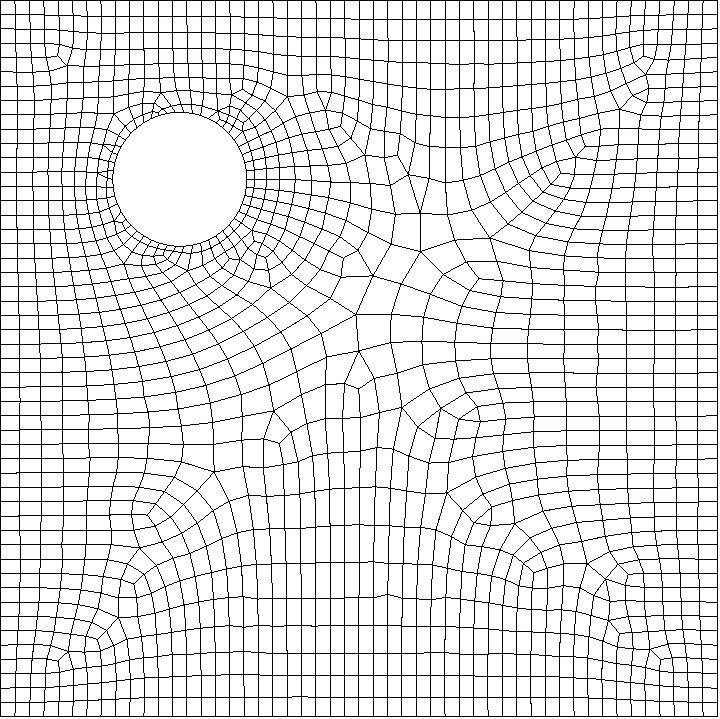
\includegraphics[height=5.0cm]{figure/conforming_t1.jpg}
	}
	\quad
	\subfigure[Conforming mesh, $t = t_2$]
	{
	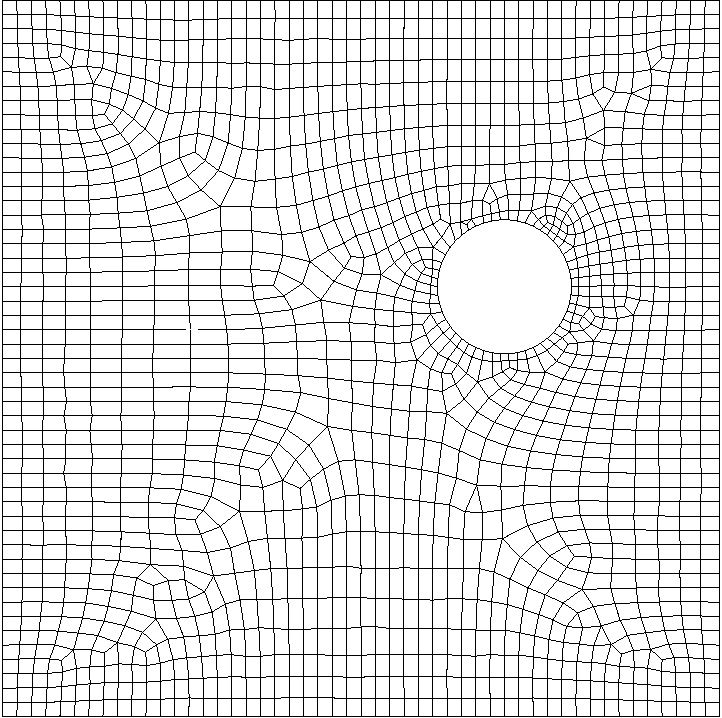
\includegraphics[height=5.0cm]{figure/conforming_t2.jpg}
	}
	\\
	\subfigure[Nonconforming mesh, $t = t_1$]
	{
	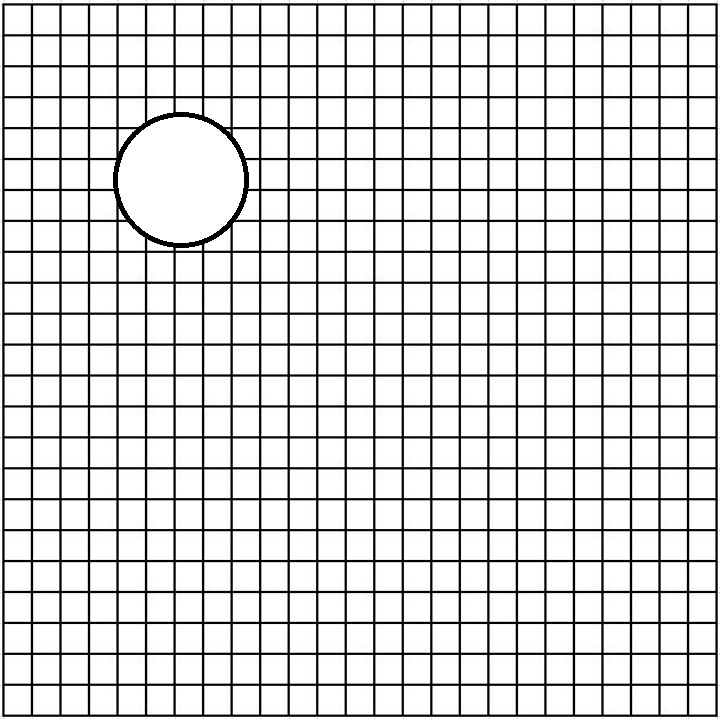
\includegraphics[height=5.0cm]{figure/nonconforming_t1.jpg}
	}
	\quad
	\subfigure[Nonconforming mesh, $t = t_2$]
	{
	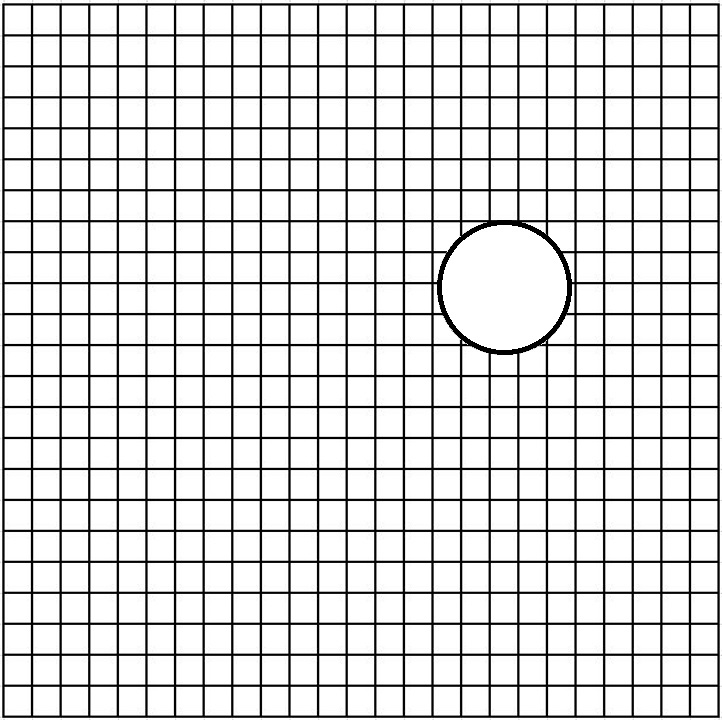
\includegraphics[height=5.0cm]{figure/nonconforming_t2.jpg}
	}
	\caption{Example of conforming and nonconforming mesh.}
	\label{fig:conformalVSnonconformal}
\end{figure}
%

Most of the non-conforming mesh methods are based upon the framework of the immersed methods. The classical IB method was firstly introduced by Peskin in 1970s \cite{peskin1972flow} to simulate blood flow in the human heart. The basic idea of an immersed boundary method is to employ a numerically efficient Cartesian grid for the discretization of the fluid phase and to represent the immersed fluid-solid interface which does not coincide with any grid line by modifications of the governing equations. This can be formulated as additional source terms in the momentum equation and can be performed in the continuous setting, i.e. before discretization, or by altering the linear system resulting from discretizing in time and space, which is termed discrete forcing \cite{mittal2005immersed}. The immersed boundary method approach is very appealing since it relieves the user from the task of grid generation which can be extremely difficult and tedious for complex configurations. In the immersed boundary method, the boundary of an immersed solid is tracked by Lagrangian markers that are convected by a fluid. Numerically, the communication between the solid and the fluid is obtained by spreading the singular forces from the Lagrangian markers to nearby Cartesian grid nodes and interpolating the velocity from nearby Cartesian grid nodes to the Lagrangian markers with the use of discrete Dirac $\delta$ functions.

The immersed boundary method has been matured and applied to different FSI problems in recent years. Choi calculated the surface pressure coefficients for a high Reynolds number around NACA0012 airfoil using the immersed boundary technique \cite{choi2007immersed}. Fadlun investigated the capability of this method to simulate high-Re turbulent flows in complex geometries. They chose an axisymmetric piston-cylinder assembly with fixed central valve for this purpose \cite{fadlun2000combined}. Mittal developed a sharp interface immersed boundary method for simulating incompressible viscous flow past three-dimensional immersed bodies. They applied it to a highly complex three-dimensional moving body of bluegill sunfish \cite{mittal2008versatile}. Their method was based on a discrete-forcing scheme that allows for a sharp representation of the immersed boundary. Vanella used the immersed boundary method for solving fluid-structure interaction problems \cite{vanella2010direct}. They tested the accuracy of their approach for the case of two falling plates. Most of the research that has been done on the immersed boundary focused on the analysis aspect of the method. There has been limited  research by the topology optimization community on the application of immersed boundary for optimization in the fluid regions. The penalization technique was used to optimize the flow field in a domain by several researchers \cite{challis2009level, pingen2010parametric, zhou2008variational, kreissl2012levelset, borrvall2003topology}. However, this technique is only applicable to low Reynolds number flows.

In this paper, we use the continuum sensitivity analysis to calculate the sensitivity of coupled fluid-solid interaction problems to shape parameters. The fluid-solid interaction is modelled using the immersed boundary method. The traditional immersed boundary method uses a discrete Dirac $\delta$ function for transferring data between the domains. This is not applicable when using continuum sensitivity analysis since the governing equations needs to be differentiable. A regularized delta function is developed to satisfy this need. The methodology is applied to two demonstration problems.

% ==========================================================================================
\section{Numerical Approach}
% -.-.-.-.-.-.-.-.-.-.-.-.-.-.-.-.-.-.-.-.-.-.-.-.-.-.-.-.-.-.-.-.-.-.-.-.-.-.-.-.-.-.-.-.-
\subsection{Immersed Boundary Formulation}
Viscous and incompressible flow in a cartesian square domain $\Omega$ containing an immersed boundary, as shown in Figure \eqref{fig:immersedBoundary}, can be modelled by the Navier-Stokes equations:

%
\begin{subequations}\label{eq:NS}
\begin{equation}
	\rho \left[
	\frac{\partial \vec{V}}{\partial t} + 
	\vec{\nabla} \cdot \left( \vec{V} \otimes \vec{V} \right) 
	\right] = 
	-\vec{\nabla} P + \mu \nabla^2 \vec{V} + \vec{F}
\end{equation}
\begin{equation}
	\vec{\nabla} \cdot \vec{V} = 0
\end{equation}
\end{subequations}
%

where $\vec{F}$ is given by

%
\begin{equation}\label{eq:forceAtEulerian}
	\vec{F}(\vec{x}, t) = \int_\Omega \vec{f} (\vec{x}_k, t) \delta(\vec{x} - \vec{x}_k) d\vec{x}_k
\end{equation}
%

and $\delta(\vec{x} - \vec{x}_k)$ is a Dirac delta function; $\vec{x}_k$ are the Lagrangian points placed over the immersed boundary; $\vec{f}(\vec{x}_k)$ is the Lagrangian force density; and $\vec{F}(\vec{x})$ is the Eulerian force that is not equal to zero only over the immersed boundary. Equation \eqref{eq:forceAtEulerian} models the interaction between the immersed boundary and the fluid flow by injecting a force field on the fluid. The Lagrangian force terms are calculated using virtual boundary formulation that is proposed by Goldstein \cite{goldstein1993modeling} which was used to simulate turbulent flow over a riblet-covered surface and to address other similar problems. The main idea of this method is to treat the embedded boundary in the fluid by adding a force field to the fluid, taking the same velocity as the surface. Since the force field is not known a priori, it must be calculated in a feedback way such that the velocity on the boundary is used to determine the desired force distribution. This model involves two imposed constants, $\alpha$ and $\beta$, which are chosen to be both negative and large enough in magnitude to bring the fluid velocity close to the interface velocity. The feedback forcing function $\vec{f}(\vec{x}_k)$ can assume the expression as

%
\begin{equation}\label{eq:forcingFunction}
	\vec{f}\left( \vec{x}_k, t \right) = 
	\alpha \int_0^t \left[ \vec{u}\left( \vec{x}_k, t \right) - \vec{U}\left( \vec{x}_k, t \right) \right]dt + 
	\beta \left[ \vec{u}\left( \vec{x}_k, t \right) - \vec{U}\left( \vec{x}_k, t \right) \right]
\end{equation}
%

where $\alpha$ and $\beta$ are constants that must be adjusted in order to obtain the expected physical behaviour at the flow. $\vec{u}\left( \vec{x}_k, t \right)$ is the value of the response variable from the Eulerian nodes calculated at the Lagrangian nodes. $\vec{U}\left( \vec{x}_k, t \right)$ is the desired value of $\vec{u}\left( \vec{x}_k, t \right)$ as the Lagrangian nodes, $\vec{x}_k$. For the case of a no-slip boundary condition where the velocities are zero on the immersed boundary, $\vec{U}\left( \vec{x}_k, t \right)$ is equal to zero. This means that the forcing function in Equation \eqref{eq:forcingFunction} tries to bring the velocity to zero on the surface of the immersed boundary. $\vec{u}\left( \vec{x}_k, t \right)$ can be calculated using the same delta function used in Equation \eqref{eq:forceAtEulerian}.

%
\begin{equation}\label{eq:velocityAtLagrangian}
	\vec{u}(\vec{x}_k, t) = \int_\Omega \vec{u} (\vec{x}, t) \delta(\vec{x} - \vec{x}_k) d\vec{x}
\end{equation}
%

%
\begin{figure}[H]
	\centering
	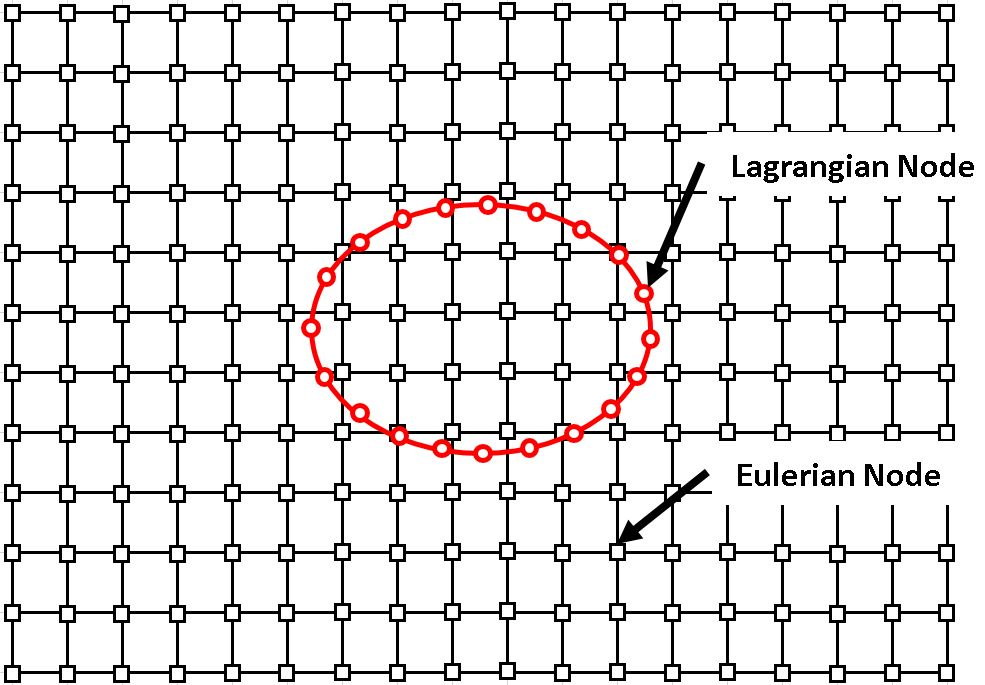
\includegraphics[height=6.0cm]{figure/immerdBoundary.jpg}
	\caption{Immersed boundary illustration}
	\label{fig:immersedBoundary}
\end{figure}
%

As shown in Equation \eqref{eq:forceAtEulerian}, the regularized delta function is used to transfer quantities between Lagrangian and Eulerian locations in Equation \eqref{eq:forceAtEulerian}. Shin investigated the stability of virtual boundary formulation for various types of regularized delta functions \cite{shin2008assessment}. However, the regularized delta functions used were not continuously differentiable. This is a requirement for continuum sensitivity analysis approach since the governing equations need to be differentiated to get the sensitivity equations. Therefore, we propose the following regularized delta function formulation:

%
\begin{equation}\label{eq:heavisideFunction}
	\delta_h(\vec{x}) = \frac{1}{h^3} \phi \left( \frac{x - x_k}{h} \right)
									 \phi \left( \frac{y - y_k}{h} \right)
									 \phi \left( \frac{z - z_k}{h} \right)
\end{equation}
%

where

%
\begin{equation}\label{eq:continuousDeltaFunction}
	\phi(r) = \frac{\kappa e^{-\kappa r}}{\left( 1 + e^{-\kappa r} \right)^2} \quad , \quad r = \frac{x - x_k}{h}
\end{equation}
%

The comparison between the different delta functions is shown in Figure \ref{fig:heavisideComparison}. As shown here, the proposed function in Equation \eqref{eq:heavisideFunction} is a $\mathcal{C}^1$ compared to the regularized functions used in the literature. This is necessary for the continuum sensitivity analysis formulation. The accuracy of the proposed delta function compared to what is available in the literature is investigated in the results section. It is shown that the proposed function has the same accuracy compared to the functions used in the literature.

%
\begin{figure}
	\centering
	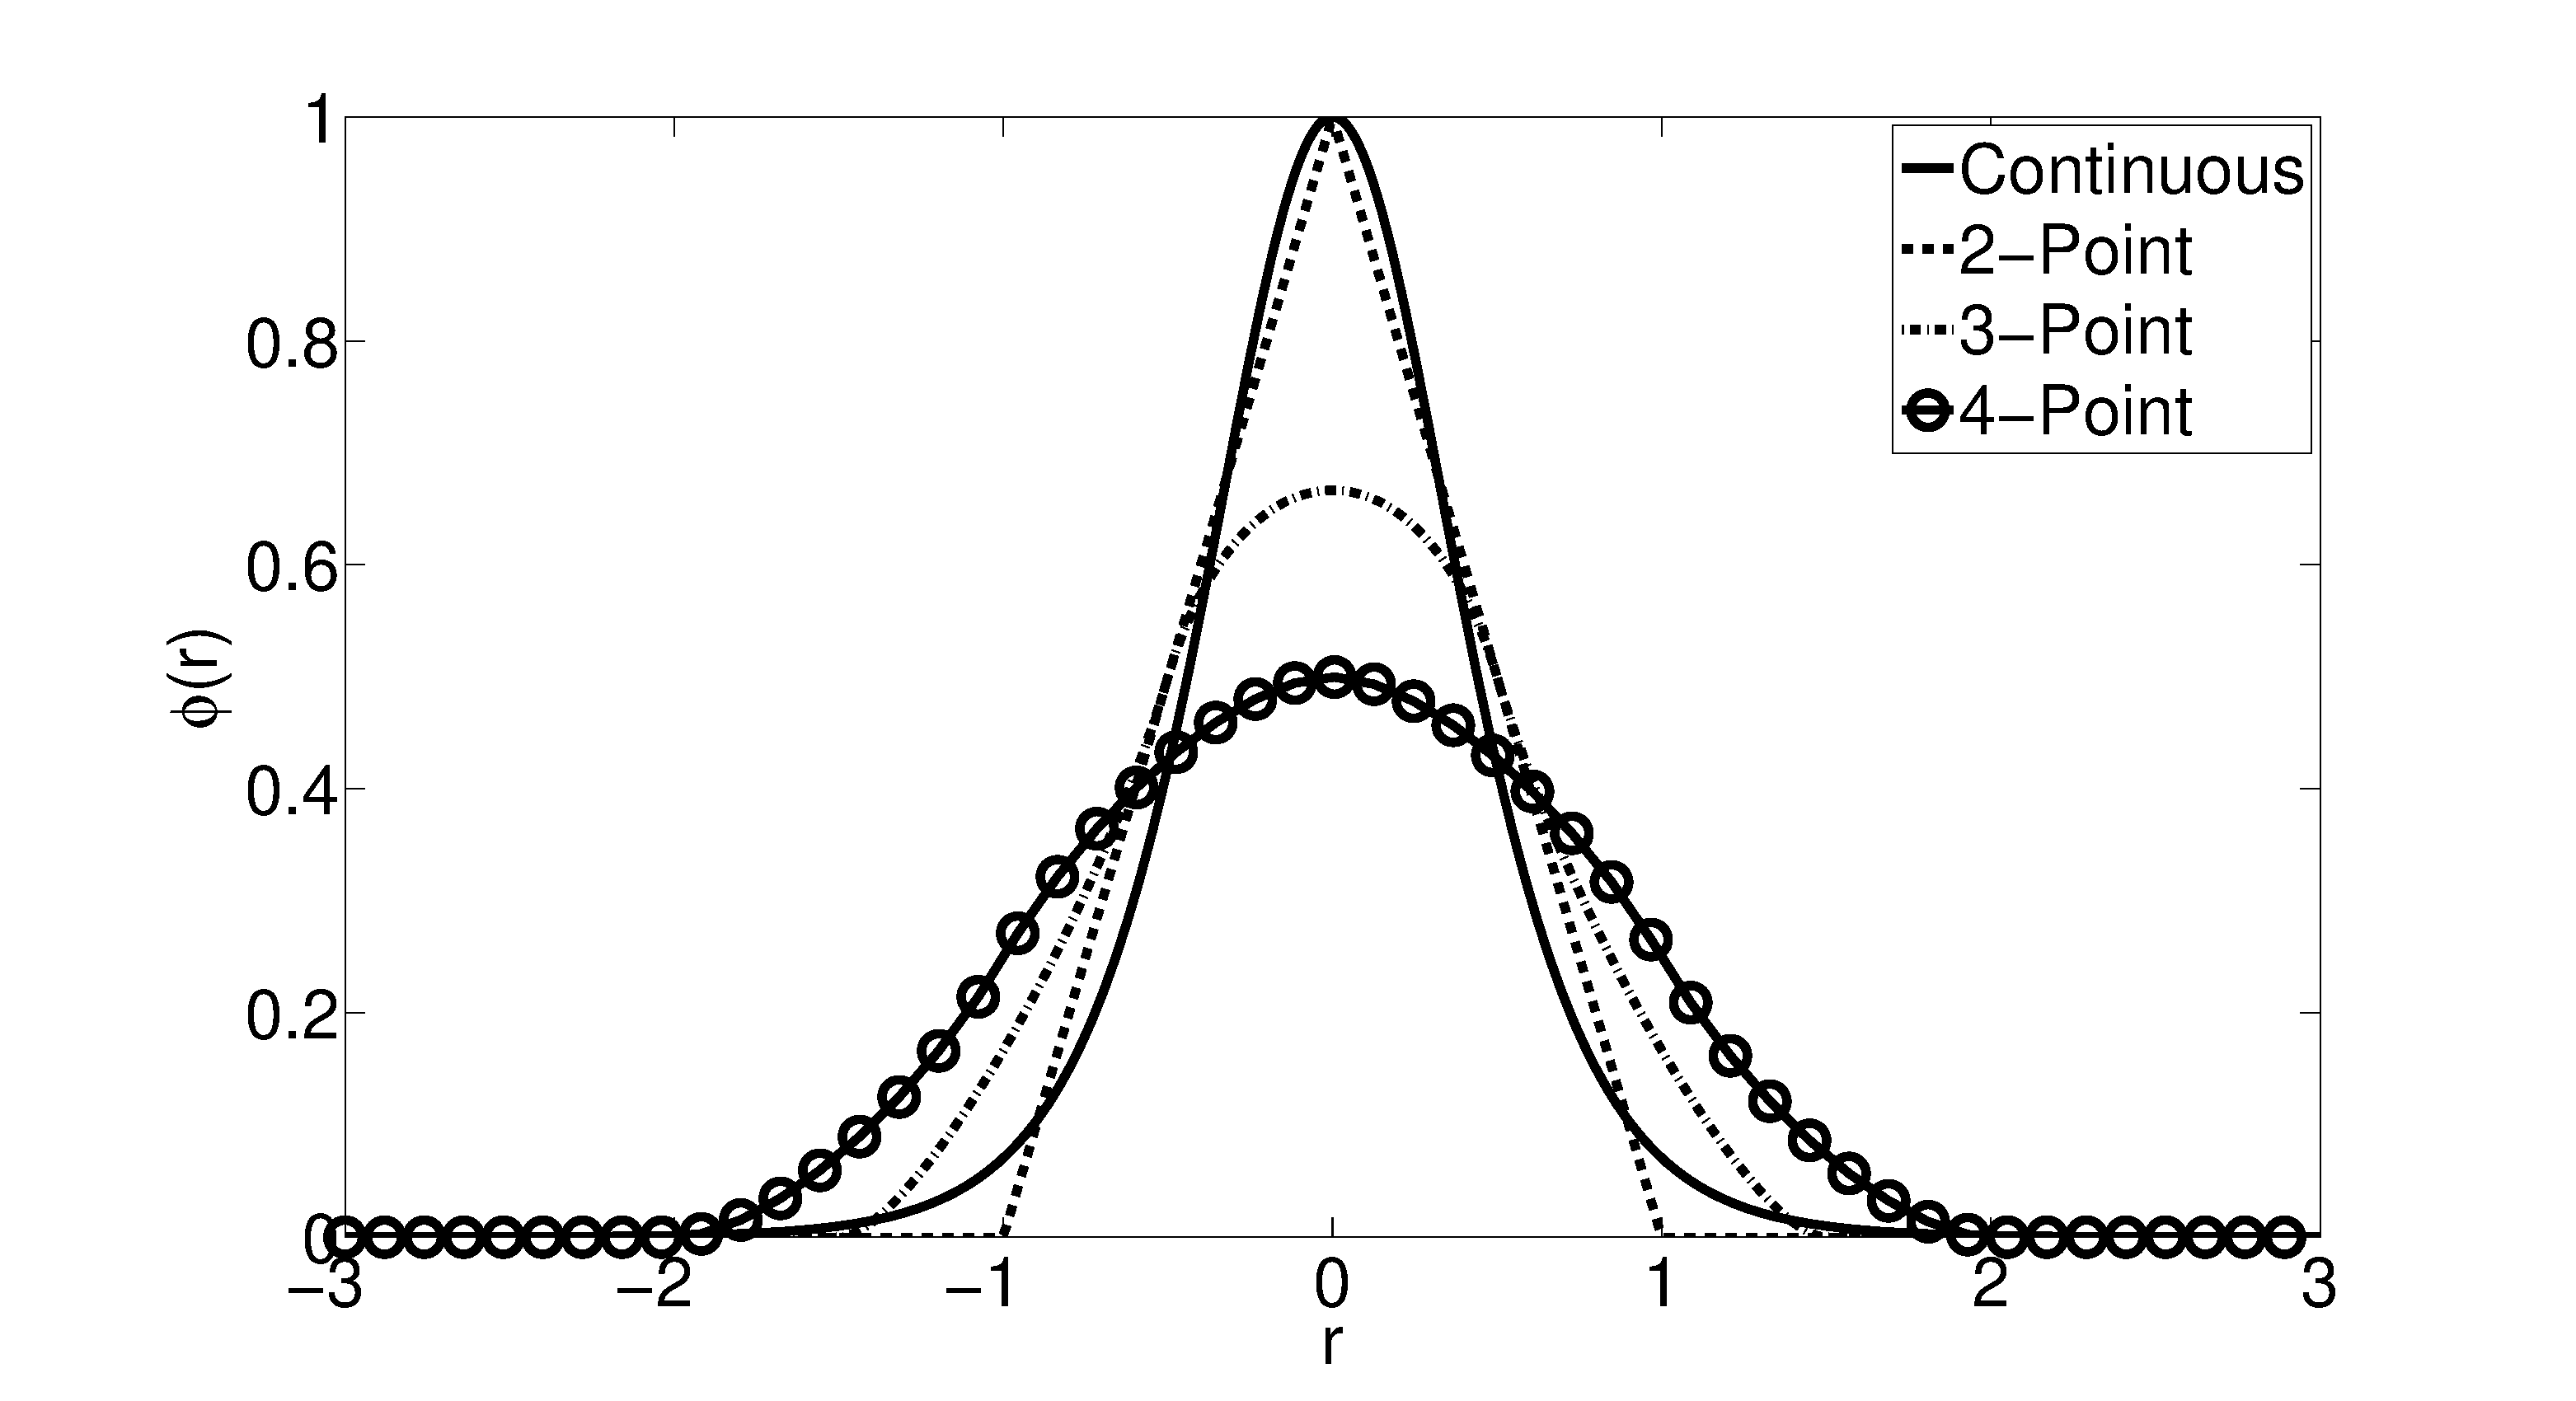
\includegraphics[height=6.0cm]{figure/heaviside_comparison.eps}
	\caption{Comparison between the different delta function formulation.}
	\label{fig:heavisideComparison}
\end{figure}
%

Finally the forcing function, $\vec{F}(\vec{x})$, can be written by combining equations \eqref{eq:forceAtEulerian}, \eqref{eq:forcingFunction}, and \eqref{eq:velocityAtLagrangian}.

%
\begin{equation}
\begin{aligned}\label{eq:forceAtEulerianFinal}
	\vec{F}(\vec{x}, t) = 
	\int_\Omega 
	&\left\{
 	\alpha \int_0^t
	\left[
	\int_\Omega \vec{u} (\vec{x}, t) \delta(\vec{x} - \vec{x}_k) d\vec{x} - \vec{U}\left( \vec{x}_k, t \right)
	\right]dt + \right. \\
	&\left.
	\beta \left[
	\int_\Omega \vec{u} (\vec{x}, t) \delta(\vec{x} - \vec{x}_k) d\vec{x} - \vec{U}\left( \vec{x}_k, t \right)
	\right]
	\right\} \delta(\vec{x} - \vec{x}_k) d\vec{x}_k
\end{aligned}
\end{equation}
%

As can be seen in above equation, the integrals on the domain $\Omega$ transfer the date between the Lagrangian and Eulerian domain. The inner integrals transfer the velocities from Eulerian to Lagrangian nodes to calculate the force at Lagrangian node, $\vec{f}\left( \vec{x}, t \right)$. The outer integral maps the forceing function from the Lagrangian to Eulerian nodes where the governing equations are solved. This is shown in Figure \ref{fig:mappingDataE2L}.

%
\begin{figure}[H]
	\centering
	\subfigure[Calculate the velocity at the Lagrangian node.]
	{
	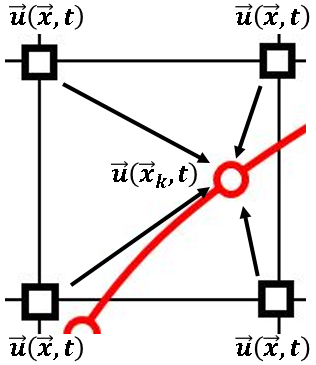
\includegraphics[height=5.0cm]{figure/mapping_1.png}
	}
	\quad
	\subfigure[Evaluate the forcing function.]
	{
	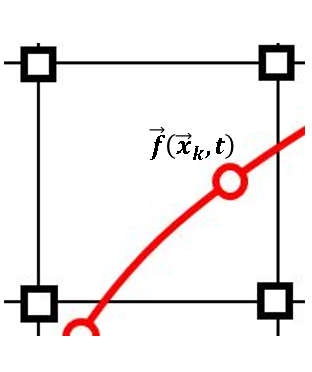
\includegraphics[height=5.0cm]{figure/mapping_2.png}
	}
	\quad
	\subfigure[Transfer the forcing function to the Eulerian nodes.]
	{
	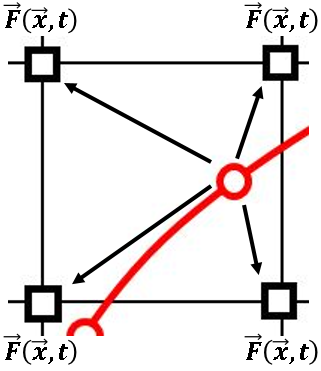
\includegraphics[height=5.0cm]{figure/mapping_3.png}
	}
	\caption{Transferring data between Eulerian and Lagrangian nodes..}
	\label{fig:mappingDataE2L}
\end{figure}
%

% -.-.-.-.-.-.-.-.-.-.-.-.-.-.-.-.-.-.-.-.-.-.-.-.-.-.-.-.-.-.-.-.-.-.-.-.-.-.-.-.-.-.-.-.-
\subsection{Analytic Sensitivity Formulation}
Figure \ref{fig:domain} represents the domain, $\Omega$, in the Cartesian space. This domain is the union of the solid, $\Omega_s$, and fluid, $\Omega_f$, domains where the Navier-Stokes equations are solved. The boundary conditions are defined on the sides of this domain, $\Gamma$. In this work, we assume that these boundary conditions do not depend on the design variables; this simplifies the derivation of the sensitivity equations. It should be noted that using this approach, the boundaries of the solid domain are added to the fluid's governing equations as mentioned in the previous section.

%
\begin{figure}[H]
	\centering
	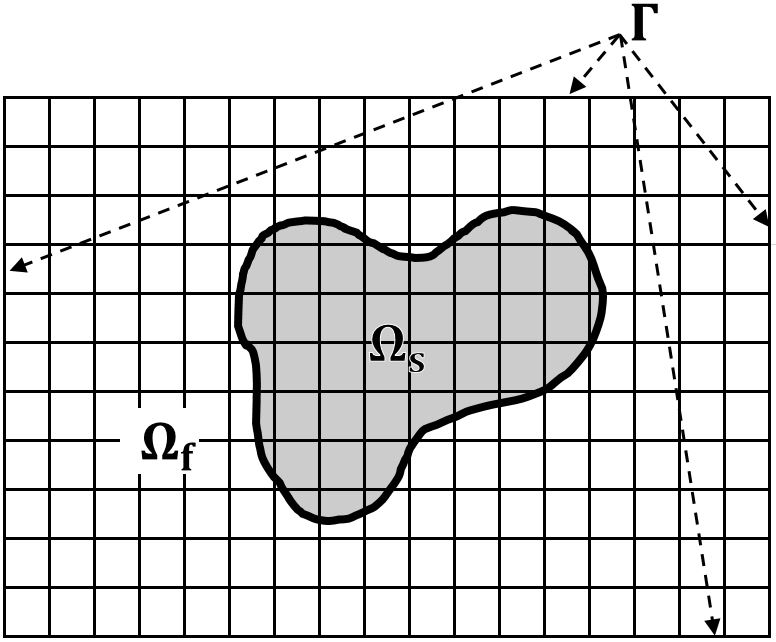
\includegraphics[height=6.0cm]{figure/domain.jpg}
	\caption{Computational domain, $\Omega = \Omega_f \cup \Omega_s$, with boundary of $\Gamma$}
	\label{fig:domain}
\end{figure}
%

The governing equation and boundary conditions can be written in the general form as

%
\begin{subequations}\label{eq:generalFormForGE}
\begin{equation}
	A(\vec{u}, \vec{b}) = f(\vec{x}, t; \vec{b}) \quad \text{on} \quad \Omega
\end{equation}
\begin{equation}
	B(\vec{u}, \vec{b}) = g(\vec{x}, t; \vec{b}) \quad \text{on} \quad \Gamma
\end{equation}
\end{subequations}
%

where $A$ and $B$ are the differential operator for the governing equations and the boundary conditions and $\vec{u}$ is the vector of response variables. This can be displacement in structural mechanics or velocity and pressures in a fluid dynamics problem. $\vec{b}$ and $\vec{x}$ are vectors of design variable and spatial coordinates respectively. The total sensitivity of response variable $\vec{u}$ to the $i$th design variable $b_i$ is calculated as

%
\begin{equation}
	\frac{D\vec{u}}{Db_i	} = \frac{\partial \vec{u}}{\partial b_i} + 
	                        \frac{\partial \vec{u}}{\partial \vec{x}} \cdot \frac{\partial \vec{x}}{\partial b_i}
\end{equation}
%

This material derivative consists of the local design derivative, $\frac{\partial \vec{u}}{\partial b_i}$, plus a convective term, $\frac{\partial \vec{u}}{\partial \vec{x}} \cdot \frac{\partial \vec{x}}{\partial b_i}$. The local design derivative is a measure of how much the response at a point changes due to change in the design parameter. The convective term tracks the movement of the material point when the spatial coordinates will change with the design variable. The geometric domain is a function of design variable in the case of conformal meshes as shown in Figure \ref{fig:conformalVSnonconformal}. However, for the case of non-body conformal meshes, the spatial coordinates will not change as the design parameter varies. Therefore, the convective term is equal to zero \cite{gobal2014continuum}. This means that the local and total form of the sensitivities are equal.

The local sensitivity equations are derived by partial differentiation of Equation \eqref{eq:NS} along with its boundary conditions. In this paper, we assumed that the boundary conditions are design independent; therefore, their derivatives are zero at the boundaries. This greatly simplifies the derivation of analytical sensitivity equations. The differentiation to $i$th design variable, $b_i$, yields the following equation for the sensitivity analysis:

%
\begin{subequations}\label{eq:NSforSA}
\begin{equation}
	\rho \left[
	\frac{\partial \vec{V^\prime}}{\partial t} + 
	\vec{\nabla} \cdot \left( \vec{V^\prime} \otimes \vec{V} + \vec{V} \otimes \vec{V^\prime} \right) 
	\right] = 
	-\vec{\nabla} P^\prime + \mu \nabla^2 \vec{V^\prime} + \vec{F^\prime}
\end{equation}
\begin{equation}
	\vec{\nabla} \cdot \vec{V^\prime} = 0
\end{equation}
\end{subequations}
%

In the above equation, $\vec{V^\prime}$ and $P^\prime$ are the local sensitivity of the velocity and pressure to $i$th design variable, $b_i$, respectively. $\vec{V}$ is calculated from the solution of the governing equations \eqref{eq:NS}. Comparing equations \eqref{eq:NS} and \eqref{eq:NSforSA}, we can see that the form of the governing and sensitivity equations are the same. Therefore, we can use the same solver for solving both of these equations. This is not possible when using the discrete formulation for the sensitivity analysis as shown in the results section.

The effect of boundary movement is introduced in Equation \eqref{eq:NSforSA} through $\vec{F^\prime}$, more specifically throught the derivative of the regularized delta function to design variable $b_i$. The derivative of the forcing function is derived as

%
\begin{equation}
\begin{aligned}\label{eq:forceingFunctionDerivative}
	\vec{F^\prime}(\vec{x}, t) = 
	\int_\Omega 
	&\left\{
 	\alpha \int_0^t
	\left[
	\int_\Omega \vec{u^\prime} (\vec{x}, t) \delta(\vec{x} - \vec{x}_k) d\vec{x} - 
	\int_\Omega \vec{u} (\vec{x}, t) \frac{\partial \delta(\vec{x} - \vec{x}_k)}{\partial \vec{x}_k} \frac{\partial \vec{x}_k}{\partial b_i} d\vec{x}
	\right]dt + \right. \\
	&\left.
	\quad \beta
	\left[
	\int_\Omega \vec{u^\prime} (\vec{x}, t) \delta(\vec{x} - \vec{x}_k) d\vec{x} - 
	\int_\Omega \vec{u} (\vec{x}, t) \frac{\partial \delta(\vec{x} - \vec{x}_k)}{\partial \vec{x}_k} \frac{\partial \vec{x}_k}{\partial b_i} d\vec{x}
	\right]
	\right\} \delta(\vec{x} - \vec{x}_k) d\vec{x}_k + \\
	\int_\Omega 
	&\left\{
 	\alpha \int_0^t
	\left[
	\int_\Omega \vec{u} (\vec{x}, t) \delta(\vec{x} - \vec{x}_k) d\vec{x} - \vec{U}\left( \vec{x}_k, t \right)
	\right]dt + \right. \\
	&\left.
	\quad \beta \left[
	\int_\Omega \vec{u} (\vec{x}, t) \delta(\vec{x} - \vec{x}_k) d\vec{x} - \vec{U}\left( \vec{x}_k, t \right)
	\right]
	\right\} \frac{\partial \delta(\vec{x} - \vec{x}_k)}{\partial \vec{x}_k} \frac{\partial \vec{x}_k}{\partial b_i} d\vec{x}_k
\end{aligned}
\end{equation}
%

where $\vec{u^\prime}\left( \vec{x}, t \right)$ is the sensitivity of velocity to design parameter $b_i$. As shown in the above equation, we used the chain rule to differentiate the regularized delta function to the design variable $b_i$. The shape design variable only affects the location of the Lagrangian points. The derivative of the Lagrangian nodes $\vec{x}_k$ to $b_i$ can be easily calculated by the problem definition since the dependency of the shape of the domain (Lagrangian nodes) and design variables are known. The derivative of the regularized delta function to the Lagrangian node $x_k$ is calculated analytically by differentiating Equation \eqref{eq:continuousDeltaFunction}. This will give us a system of differential equations for the sensitivity response of the system. This method has a significant advantage to the conventional approaches, since there is no need to calculated the sensitivity of the boundary condition or computational mesh to the design variable. In the next section we apply this methodology to two different problems.

% ==========================================================================================
\section{Demonstration Results}
In this section we will show some applications of the continuum sensitivity analysis of flow response to shape design variables. In these problems, the immersed solid boundaries are modelled using the immersed boundary formulation as mentioned in the previous section. We consider two demonstration problems: 1) flow over a cylinder 2) one-way fluid-structure coupling of flow over an airfoil. The flow is modelled as an incompressible, viscous, and laminar flow. The governing equations are discretized as shown in Equation \eqref{eq:NSdiscretized}.

%
\begin{subequations}\label{eq:NSdiscretized}
\begin{equation}
	\frac{\vec{V}^{n+1} - \vec{V}^n}{\Delta t} + 
	\left( \frac{3}{2} N\vec{V}^n - \frac{1}{2} N\vec{V}^{n-1} \right) = 
	-G p^{n + 1/2} + 
	\frac{1}{2Re} \left( L \vec{V}^{n+1} + L \vec{V}^n \right) + 
	\vec{f}^n
\end{equation}
\begin{equation}
	D \vec{V}^{n+1} = 0
\end{equation}
\end{subequations}
%

In this equation $\vec{V}$ is the velocity vector; $p$ is the pressure; $Re$ is the Reynolds number; and $\vec{f}$ is the momentum forcing applied to enforce the no-slip boundary condition along the immersed boundary. In the above equation, $N$ is the discrete convective operator; $G$ is the discrete gradient operator; $L$ is the discrete Laplacian operator; and $D$ is the discrete divergence operator. Here, $n$ denotes the $n$th time step and $\Delta t$ denotes the time increment. The discrete spatial operators $N$, $G$, $L$, and $D$ are evaluated using the second-order central finite-difference scheme. The numerical method is based on the Navier-Stokes solver, adopting the fractional-step method and a staggered Cartesian grid system. As shown above, the force terms are treated explicitly. We use the projection approach to solve this coupled system of equations \cite{brown2001accurate}.

In the following demonstration problems, we used the complex step method to verify the sensitivity results \cite{martins2003complex}. Complex step differentiation is a technique that employs complex arithmetic to obtain the numerical value of the first derivative of a real valued analytic function of a real variable, avoiding the loss of precision inherent in traditional finite differences. The complex step derivative is calculate as follows:

%
\begin{equation}\label{eq:compelxStepFormula}
	\mathcal{F}^\prime\left(u; b\right) = \frac{\text{Im}\left[ \mathcal{F}\left(u; b + ih\right) \right]}{h}
\end{equation}
%

This means that we perturb the design variable by an imaginary value of $ih$ and then look at the imaginary portion of the resulting response divided by $h$. Using the complex step method, we can choose a small step size for $h$ without loosing accuracy. Sensitivity of an analytical function in the form $F(x) = \dfrac{e^x}{\cos^3 x + \sin^3 x}$ as $x = \pi/4$ for complex step and finite difference method is shown in Figure \ref{fig:CSvsFD}. As shown in Equation \eqref{eq:compelxStepFormula}, the nomalized error in the finite difference calculation increases as the step size becomes smaller.

%
\begin{figure}[H]
	\centering
	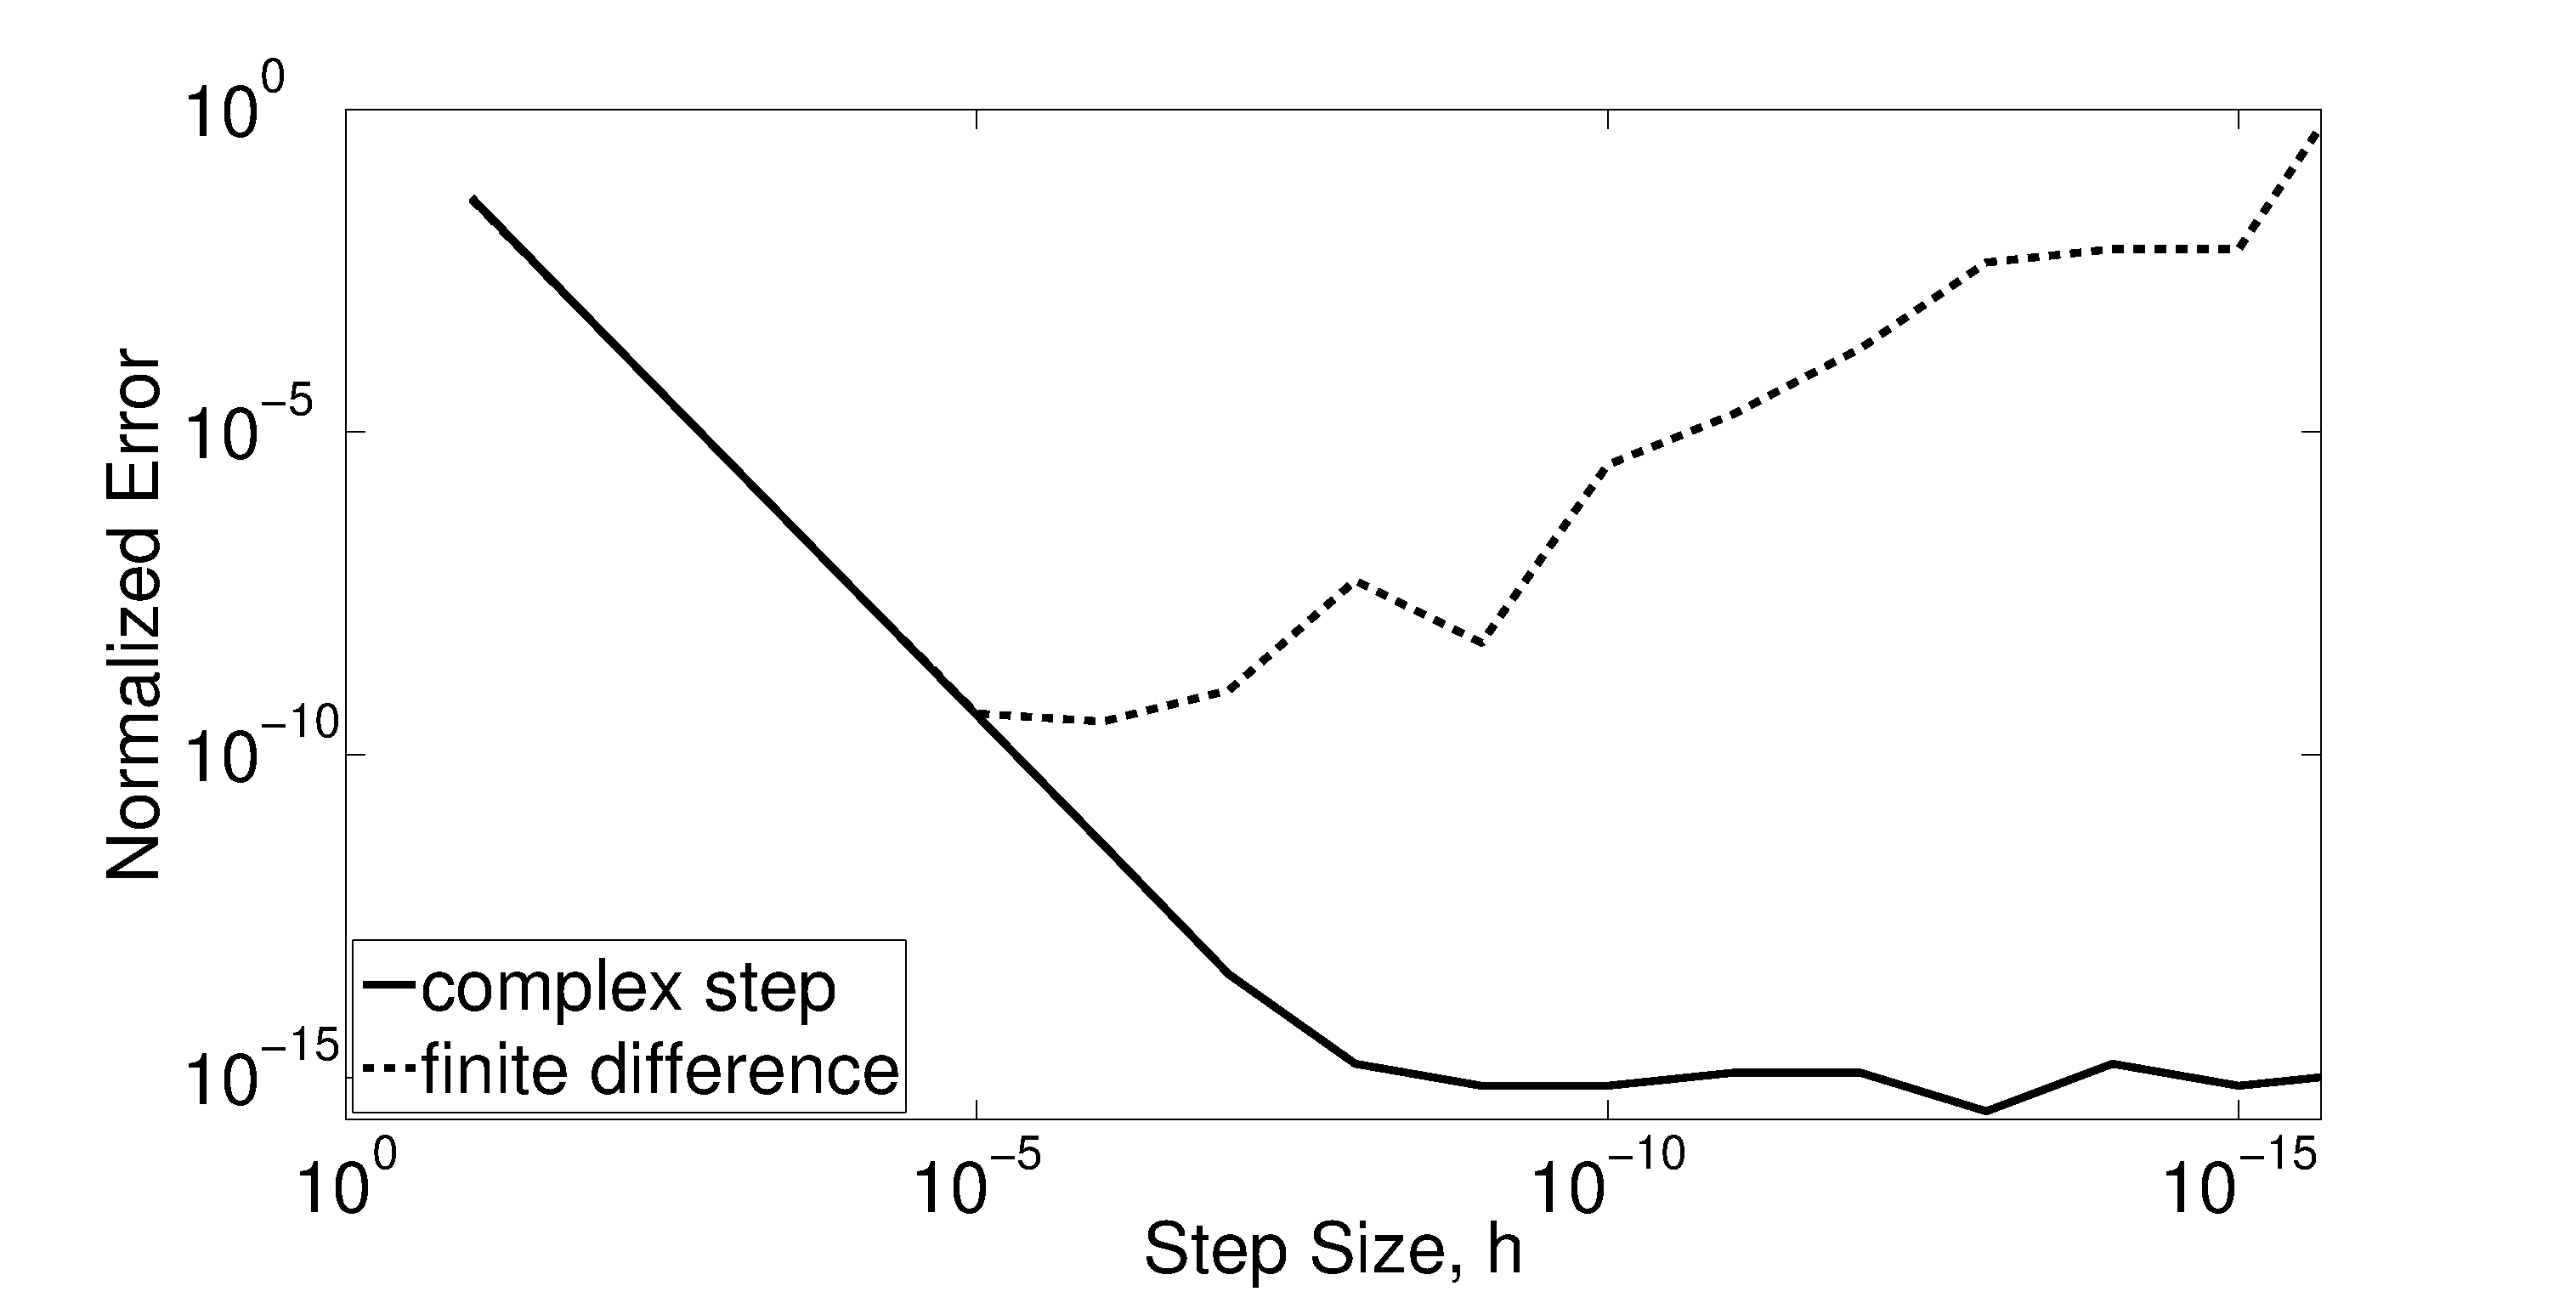
\includegraphics[height=6.0cm]{figure/FDvsCS.eps}
	\caption{Relative error in the sensitivity estimates given by the finite-difference and the complex-step methods using the analytic result as the reference. Normalized error = $\left| F^\prime - F^\prime_{ref} \right| / F^\prime_{ref}$}
	\label{fig:CSvsFD}
\end{figure}
%

% -.-.-.-.-.-.-.-.-.-.-.-.-.-.-.-.-.-.-.-.-.-.-.-.-.-.-.-.-.-.-.-.-.-.-.-.-.-.-.-.-.-.-.-.-
\subsection{Flow Over a Circular Cylinder}
We modelled the flow around the circular cylinder and calculated the sensitivity of the flow to the cylinder radius. The domain is defined as a rectangle with length and height of 2 meters and 1 meter respectively as shown in Figure \ref{fig:cylinderDomain}. The cylinder radius is selected as 0.1 meter and located 1 meter from the inlet. The inlet boundary condition is defined as constant velocity and the outlet is modelled as outflow boundary condition. This means that the gradient of $u$ and $v$ velocities are zero at the outlet. The top and bottom walls are modelled as free-slip boundary condition. The flow is modelled by choosing the Reynolds number as $100$ and $1000$. The boundary of the cylinder is modelled using 100 Lagrangian nodes. The flow results and mesh convergence study for different Reynolds numbers are shown in Figure \ref{fig:convegence_study}. For this analysis, the $\alpha$ and $\beta$ parameter of Equation \eqref{eq:forcingFunction} are selected as $-10^4$ and $-50$ respectively. As shown in Figure \ref{fig:convegence_study}, the forcing function satisfied the zero velocity condition on the surface of the cylinder.

%
\begin{figure}[H]
	\centering
	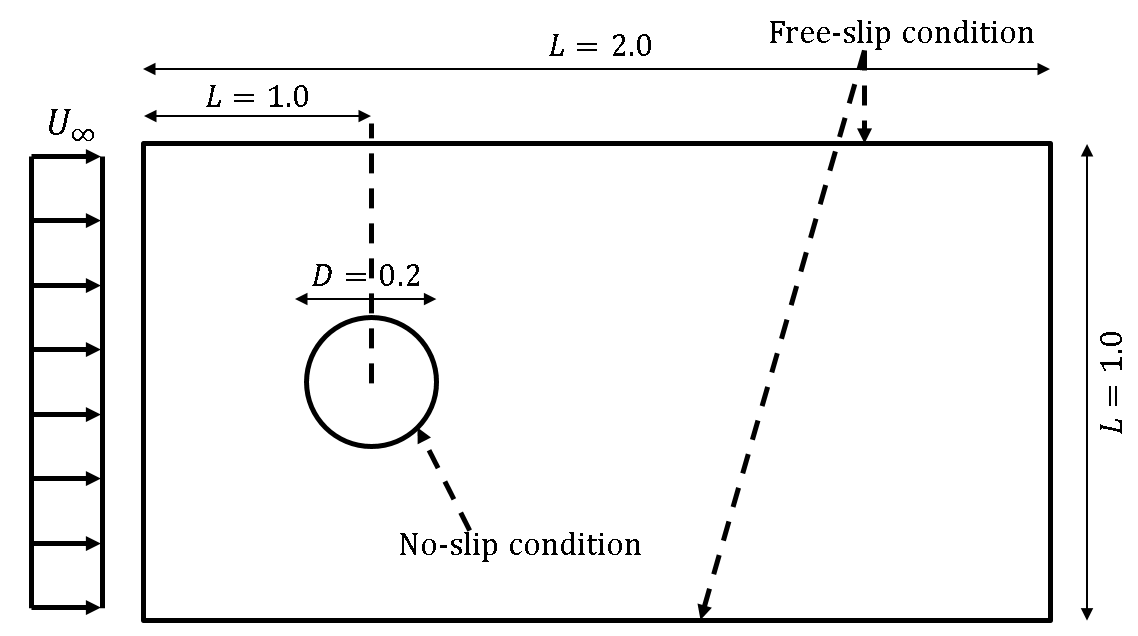
\includegraphics[height=6.0cm]{figure/cylinder/domain.png}
	\caption{Physical domain for flow over circular cylinder.}
	\label{fig:cylinderDomain}
\end{figure}
%

%
\begin{figure}[H]
	\centering
	\subfigure[Pressure contour for $Re = 100$]
	{
	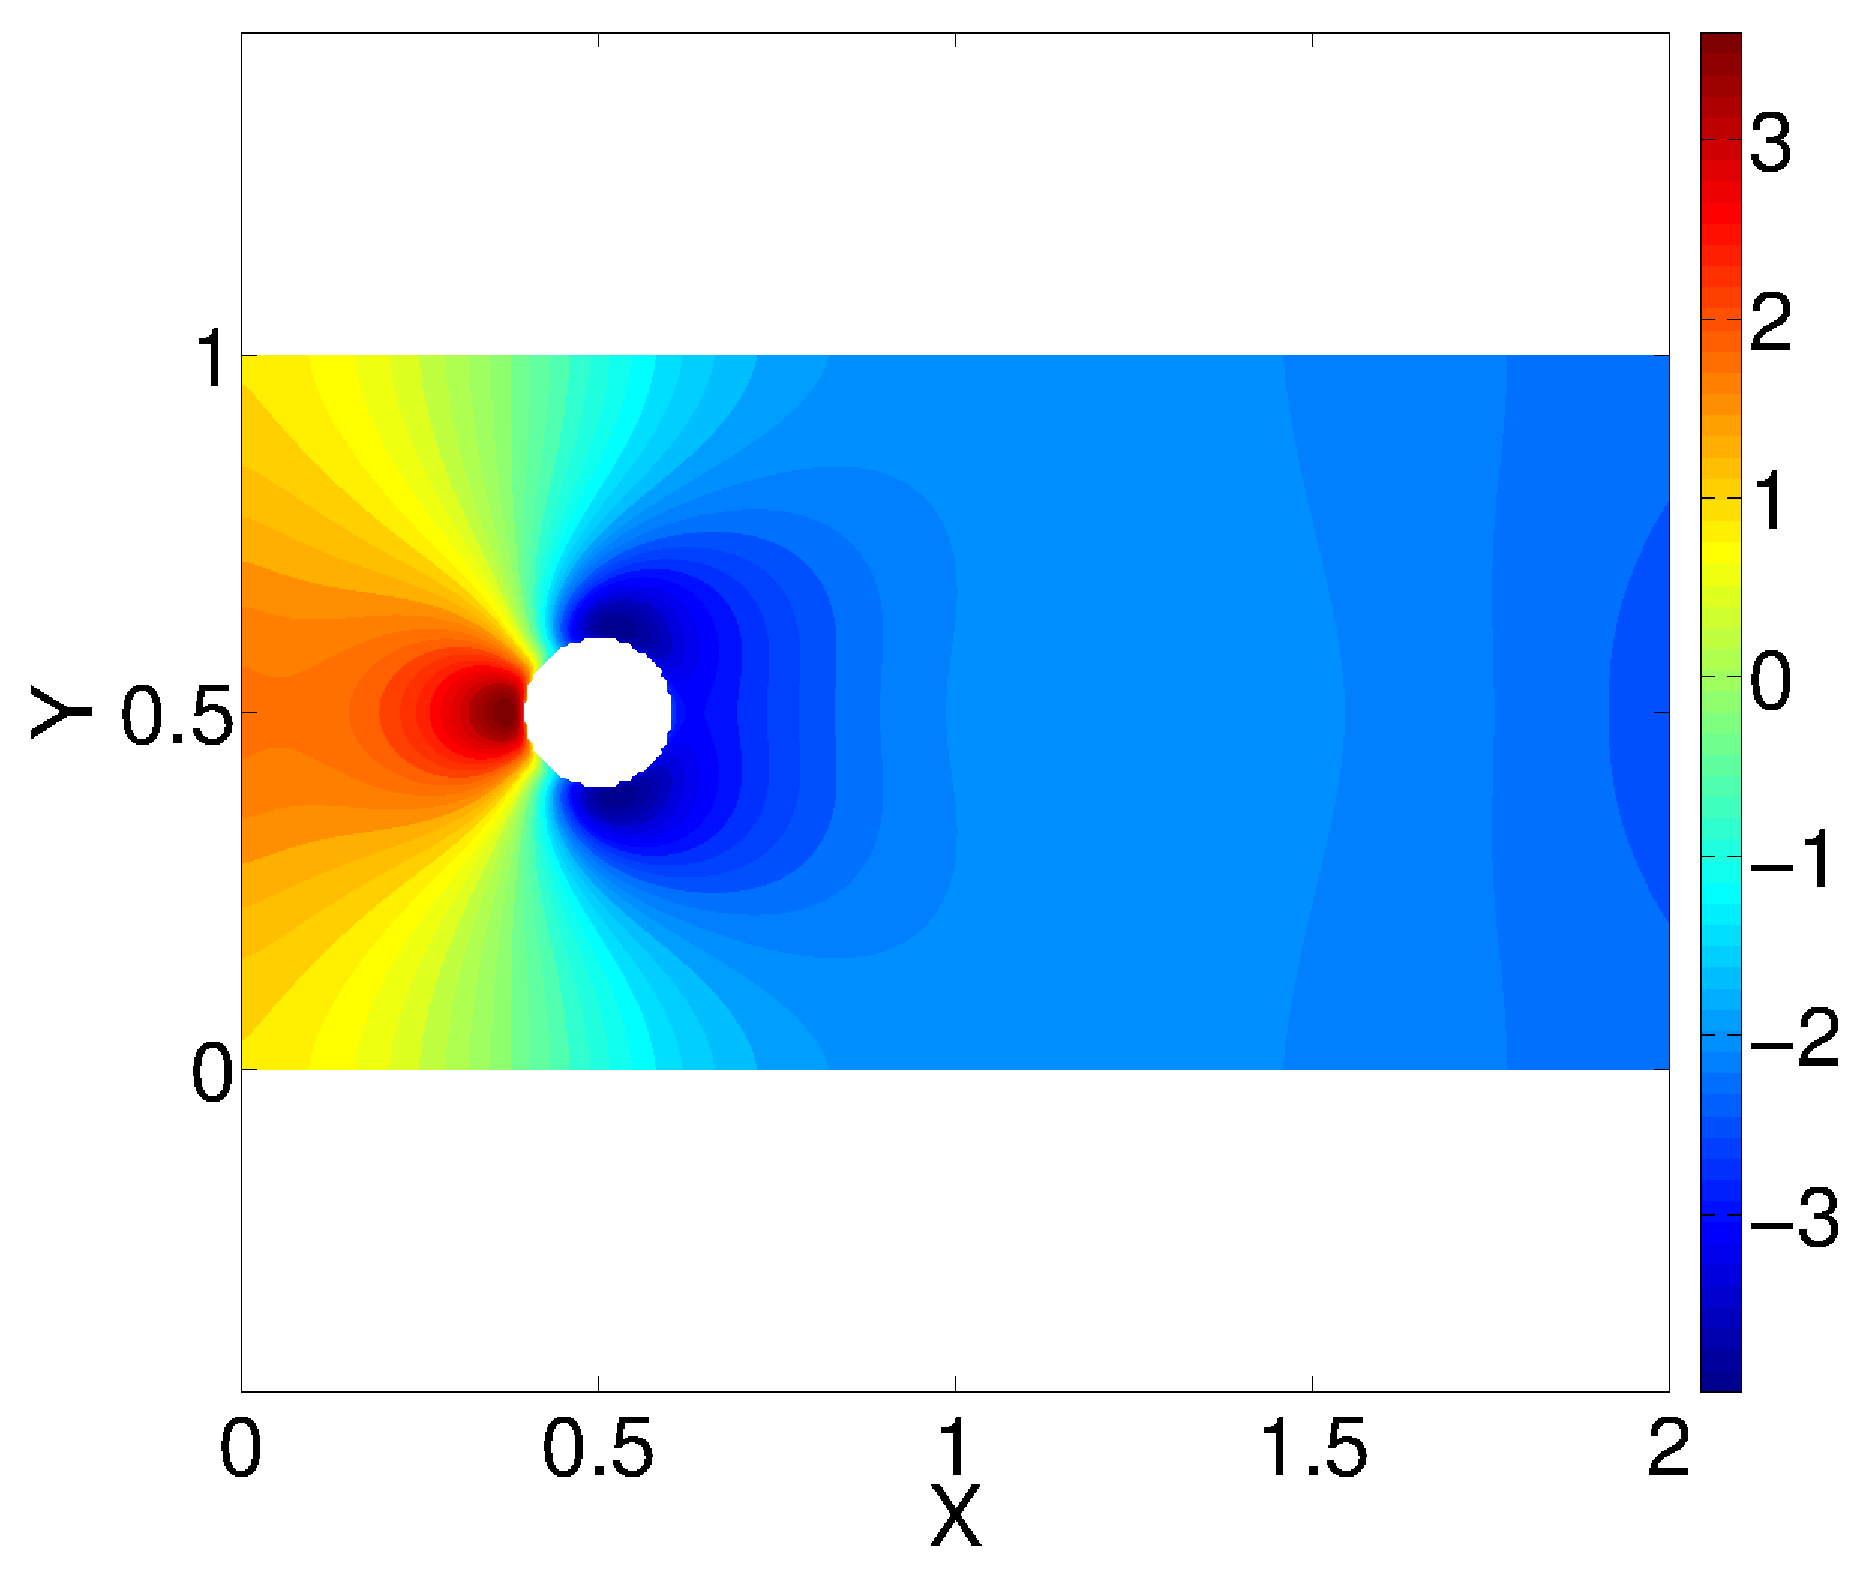
\includegraphics[height=5.0cm]{figure/cylinder/P_RE100.eps}
	}
	\quad
	\subfigure[Pressure contour for $Re = 1000$]
	{
	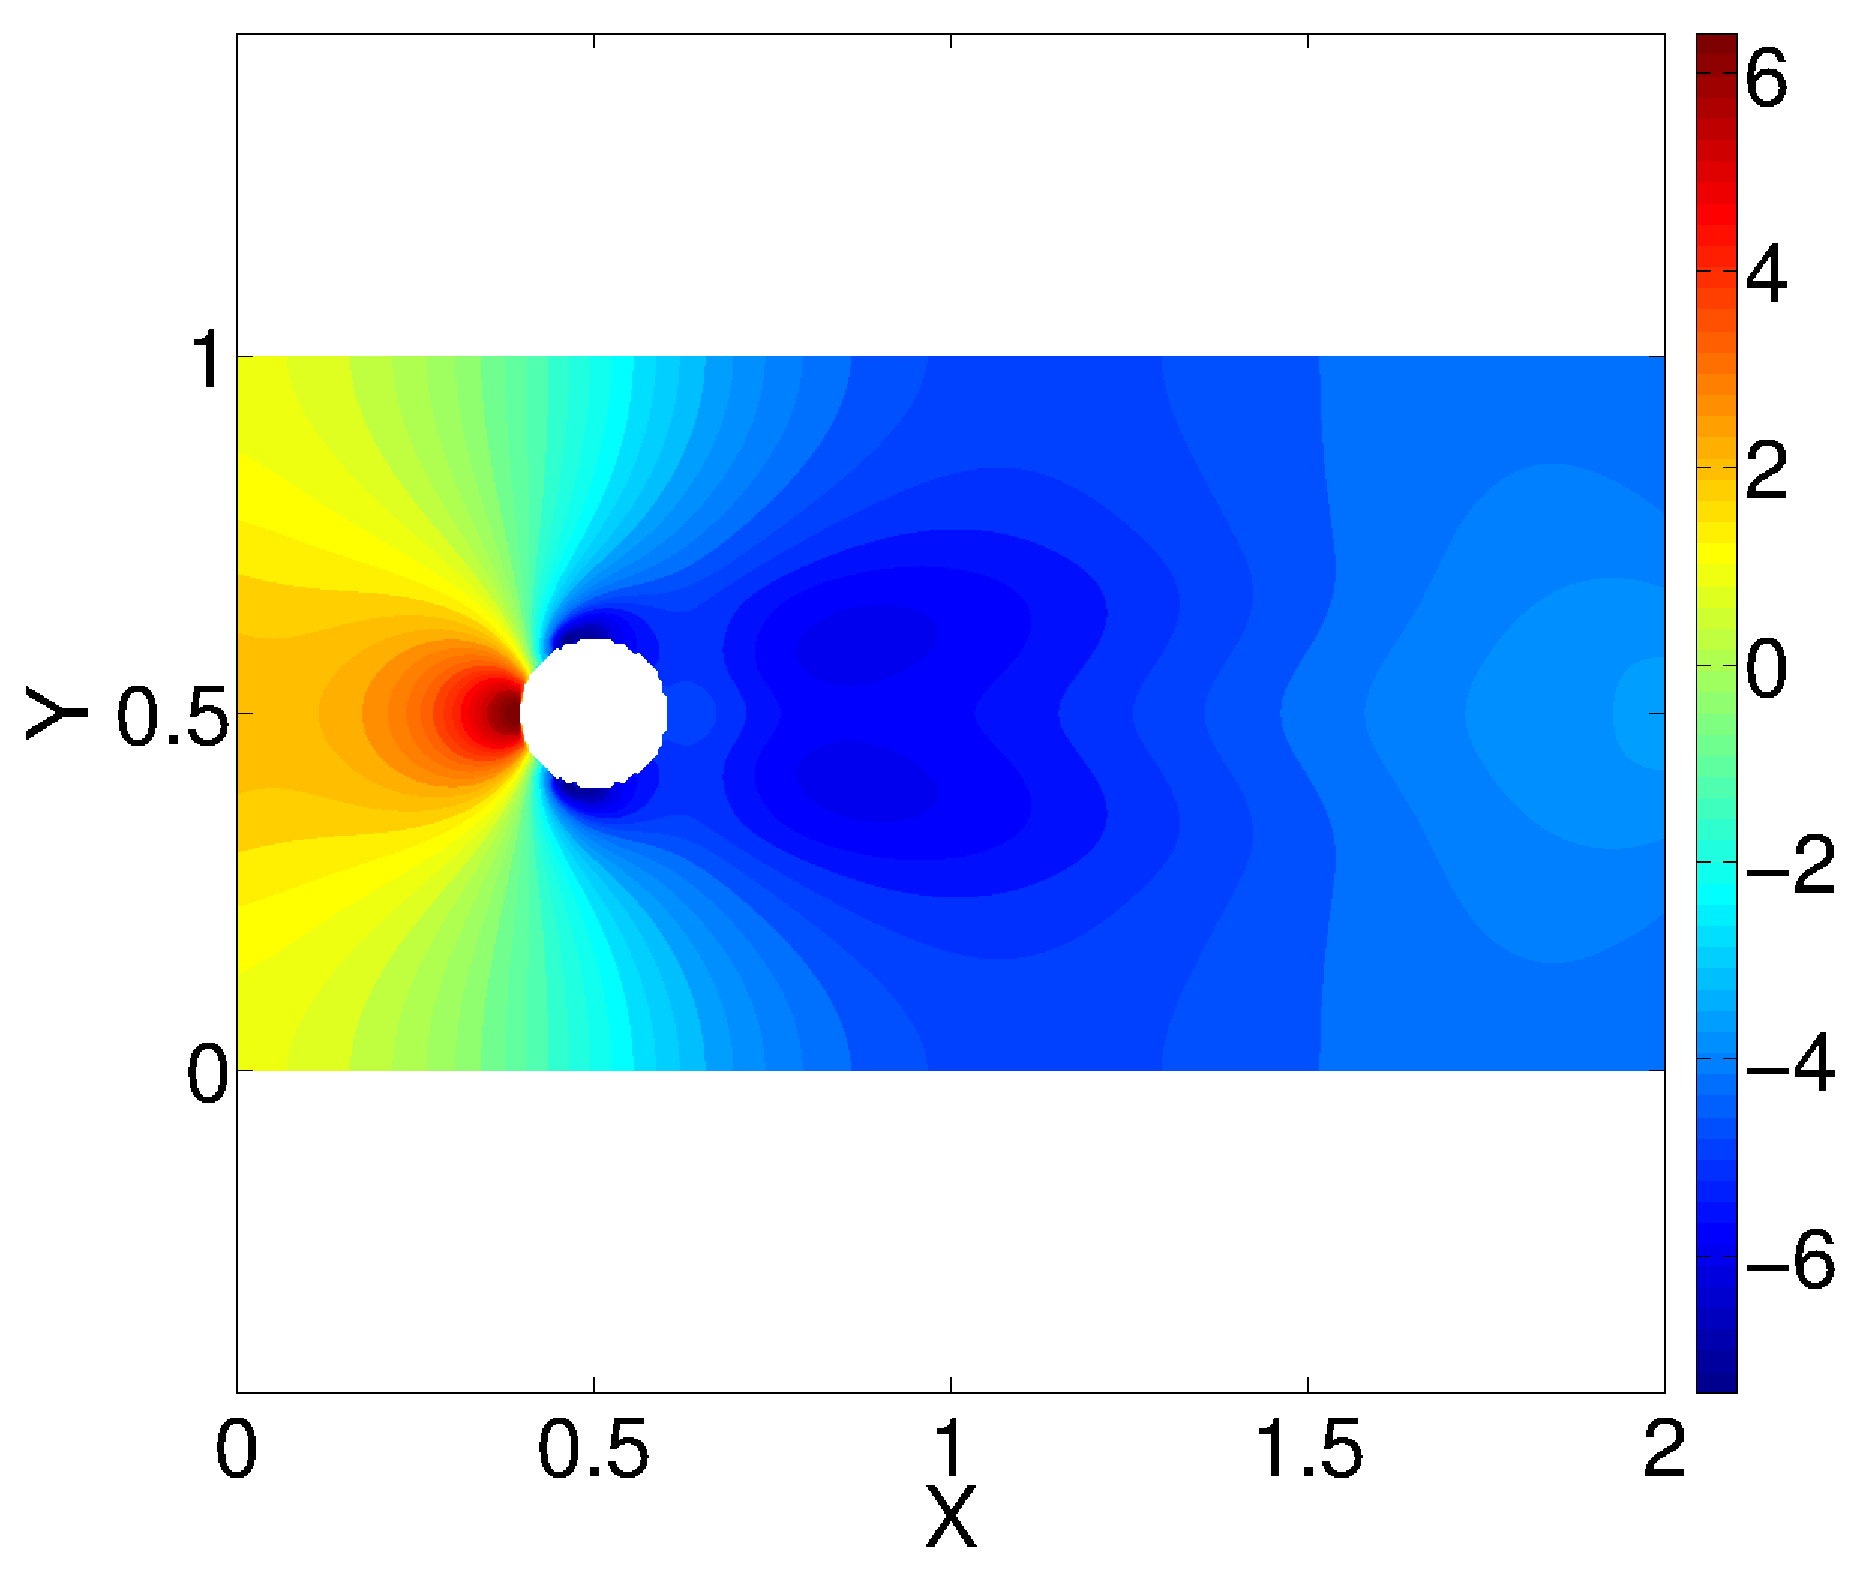
\includegraphics[height=5.0cm]{figure/cylinder/P_RE1000.eps}
	}
	\\
	\subfigure[Velocity contour for $Re = 100$]
	{
	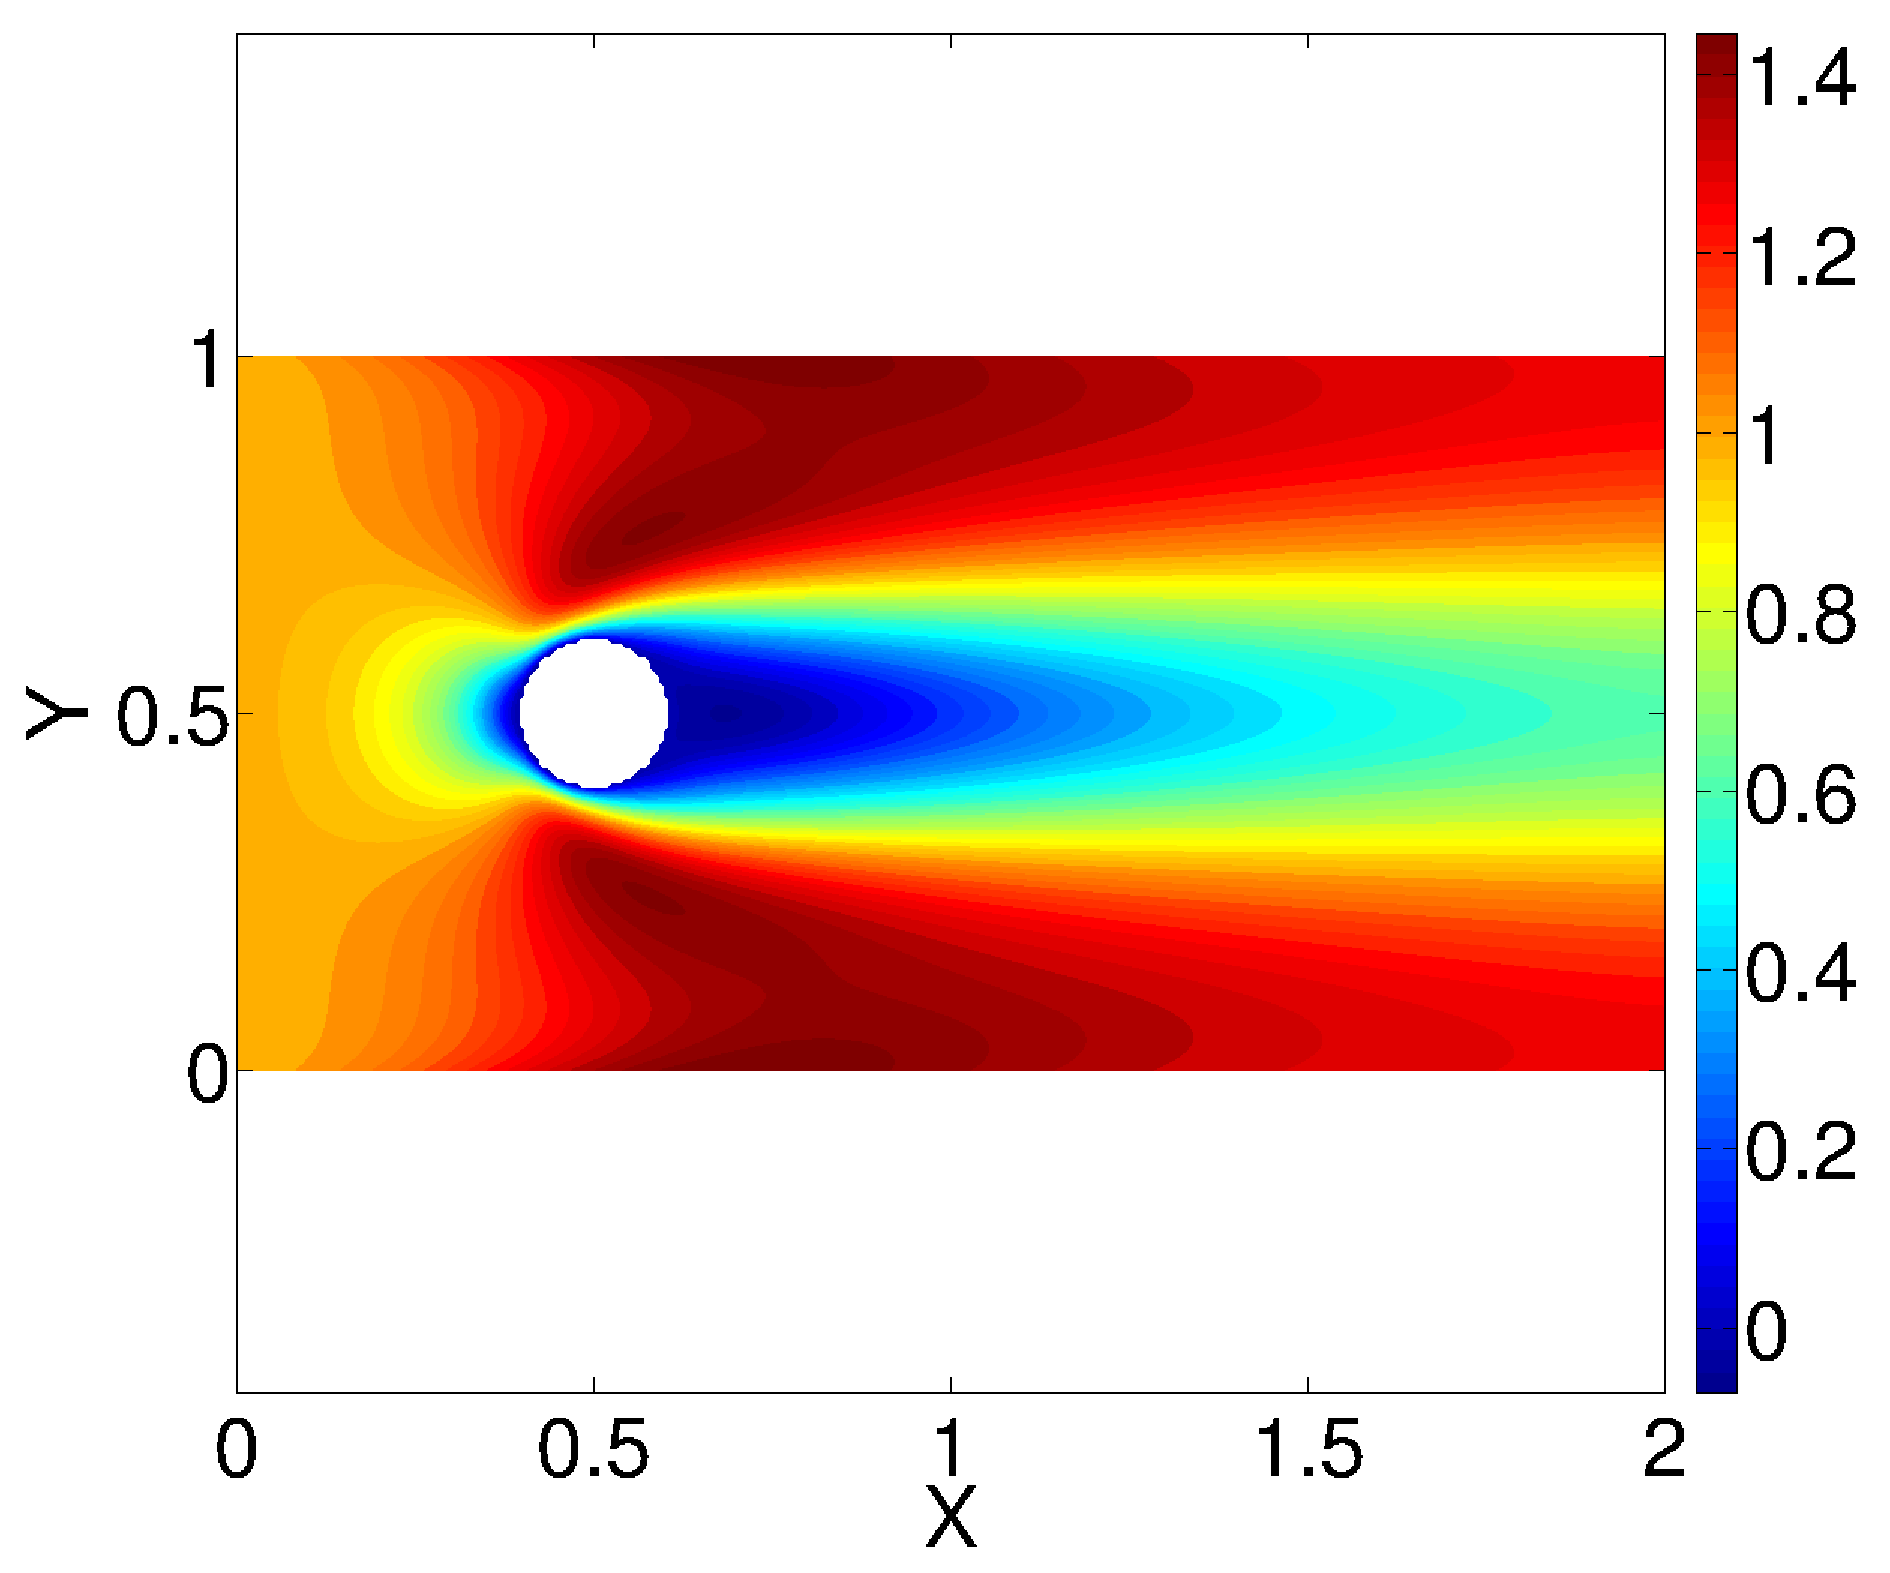
\includegraphics[height=5.0cm]{figure/cylinder/U_RE100.eps}
	}
	\quad
	\subfigure[Velocity contour for $Re = 1000$]
	{
	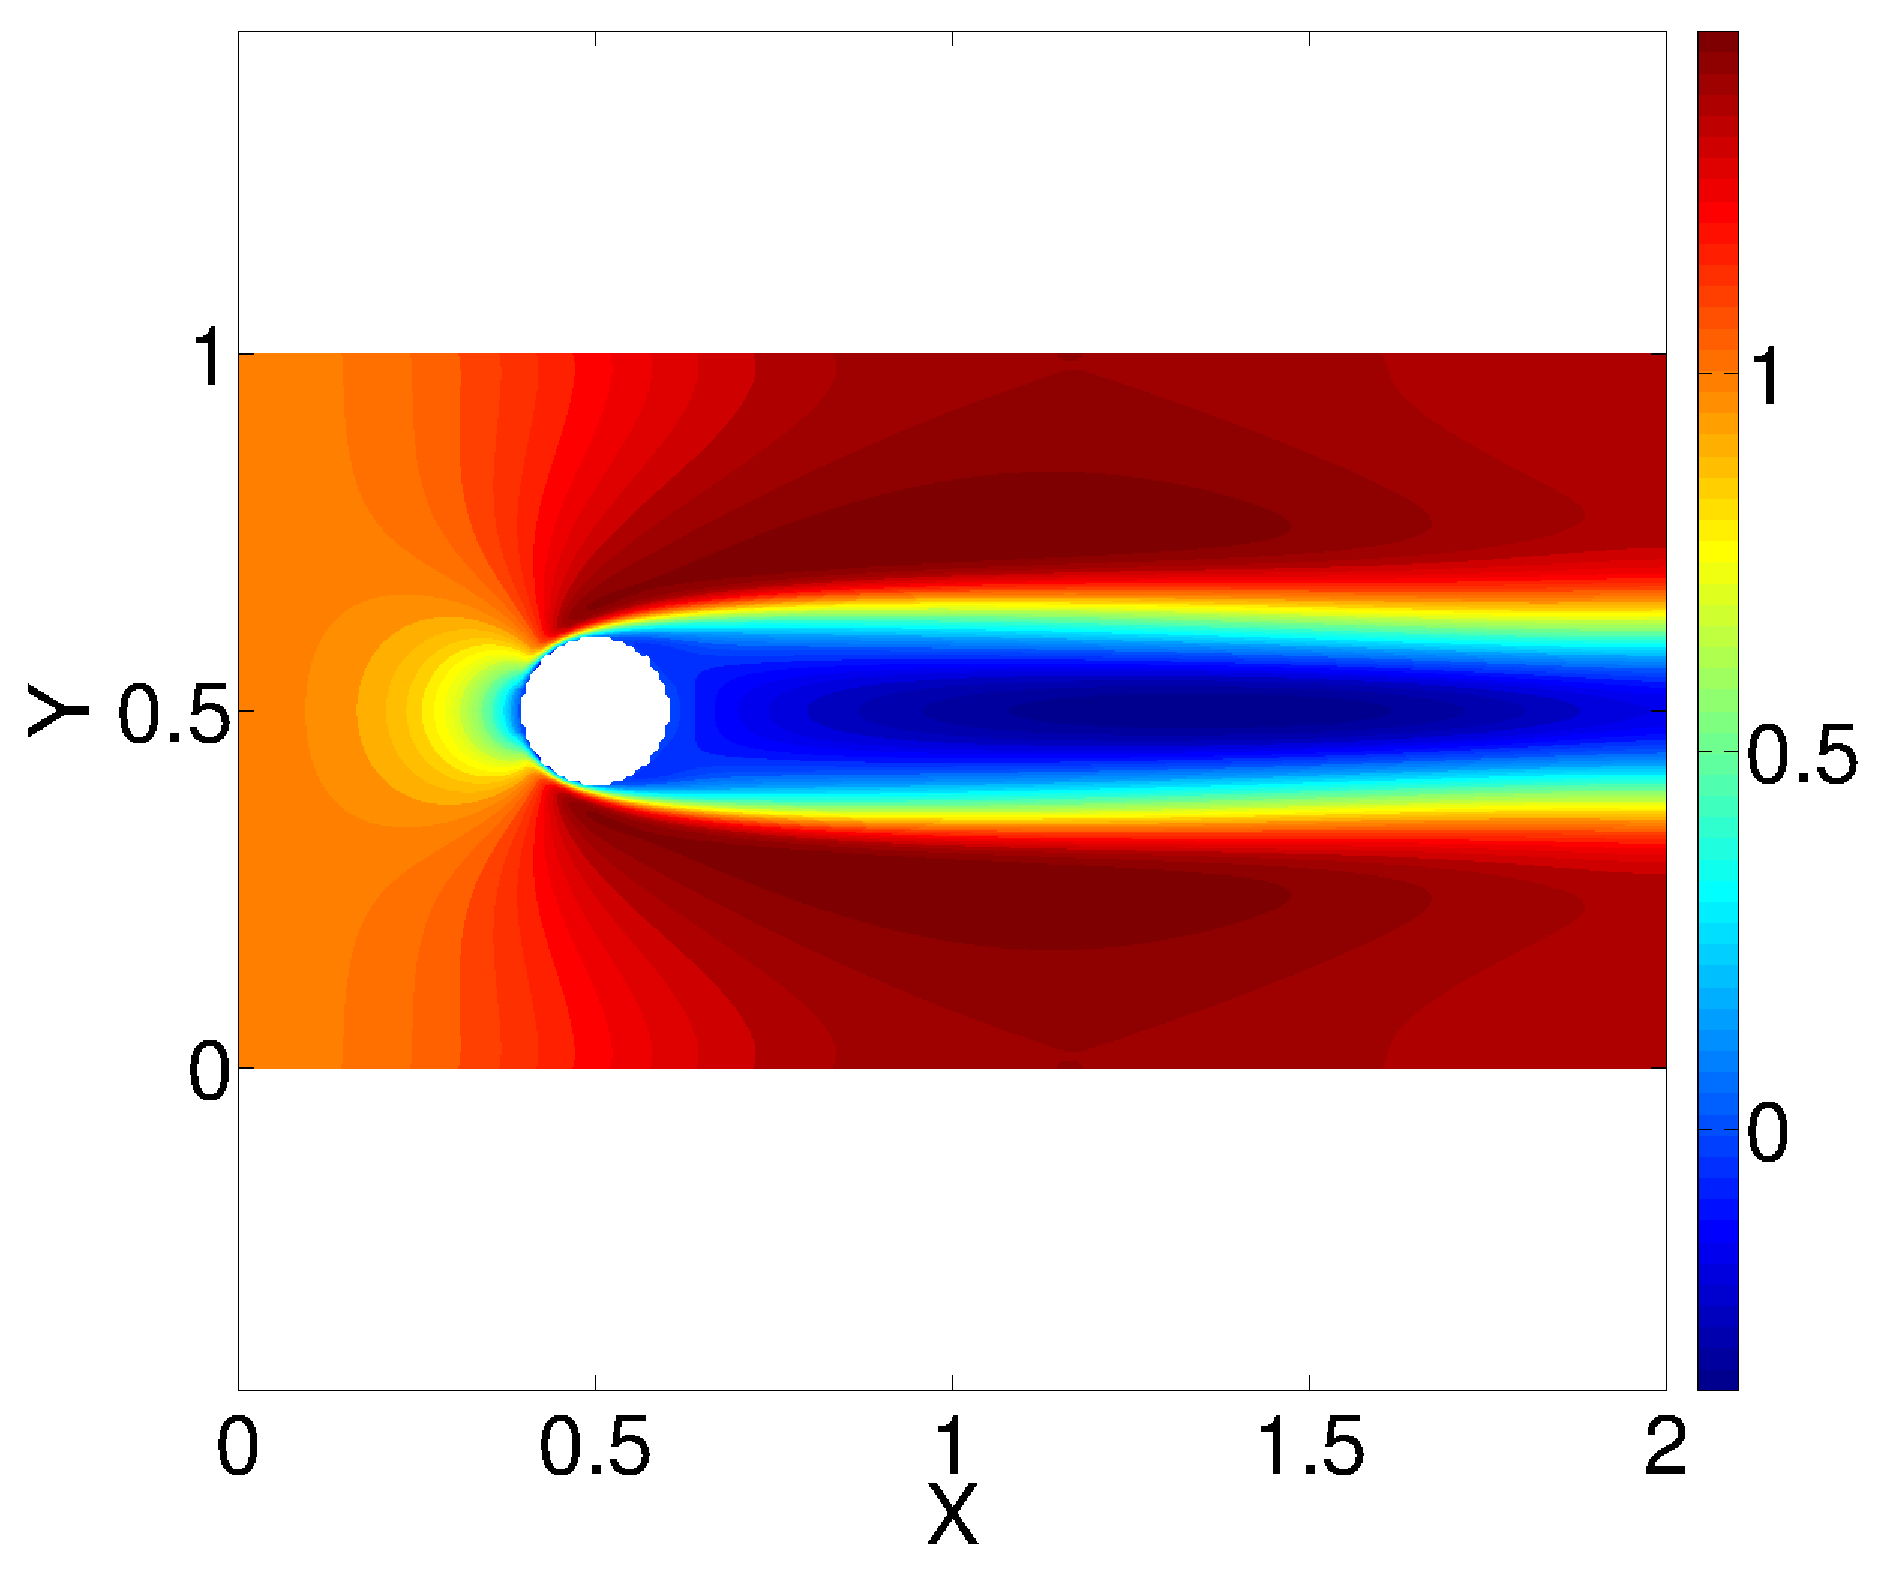
\includegraphics[height=5.0cm]{figure/cylinder/U_RE1000.eps}
	}
	\\
	\subfigure[U-velocity on $y = 0.5$ for different number of mesh nodes for $Re = 100$.]
	{
	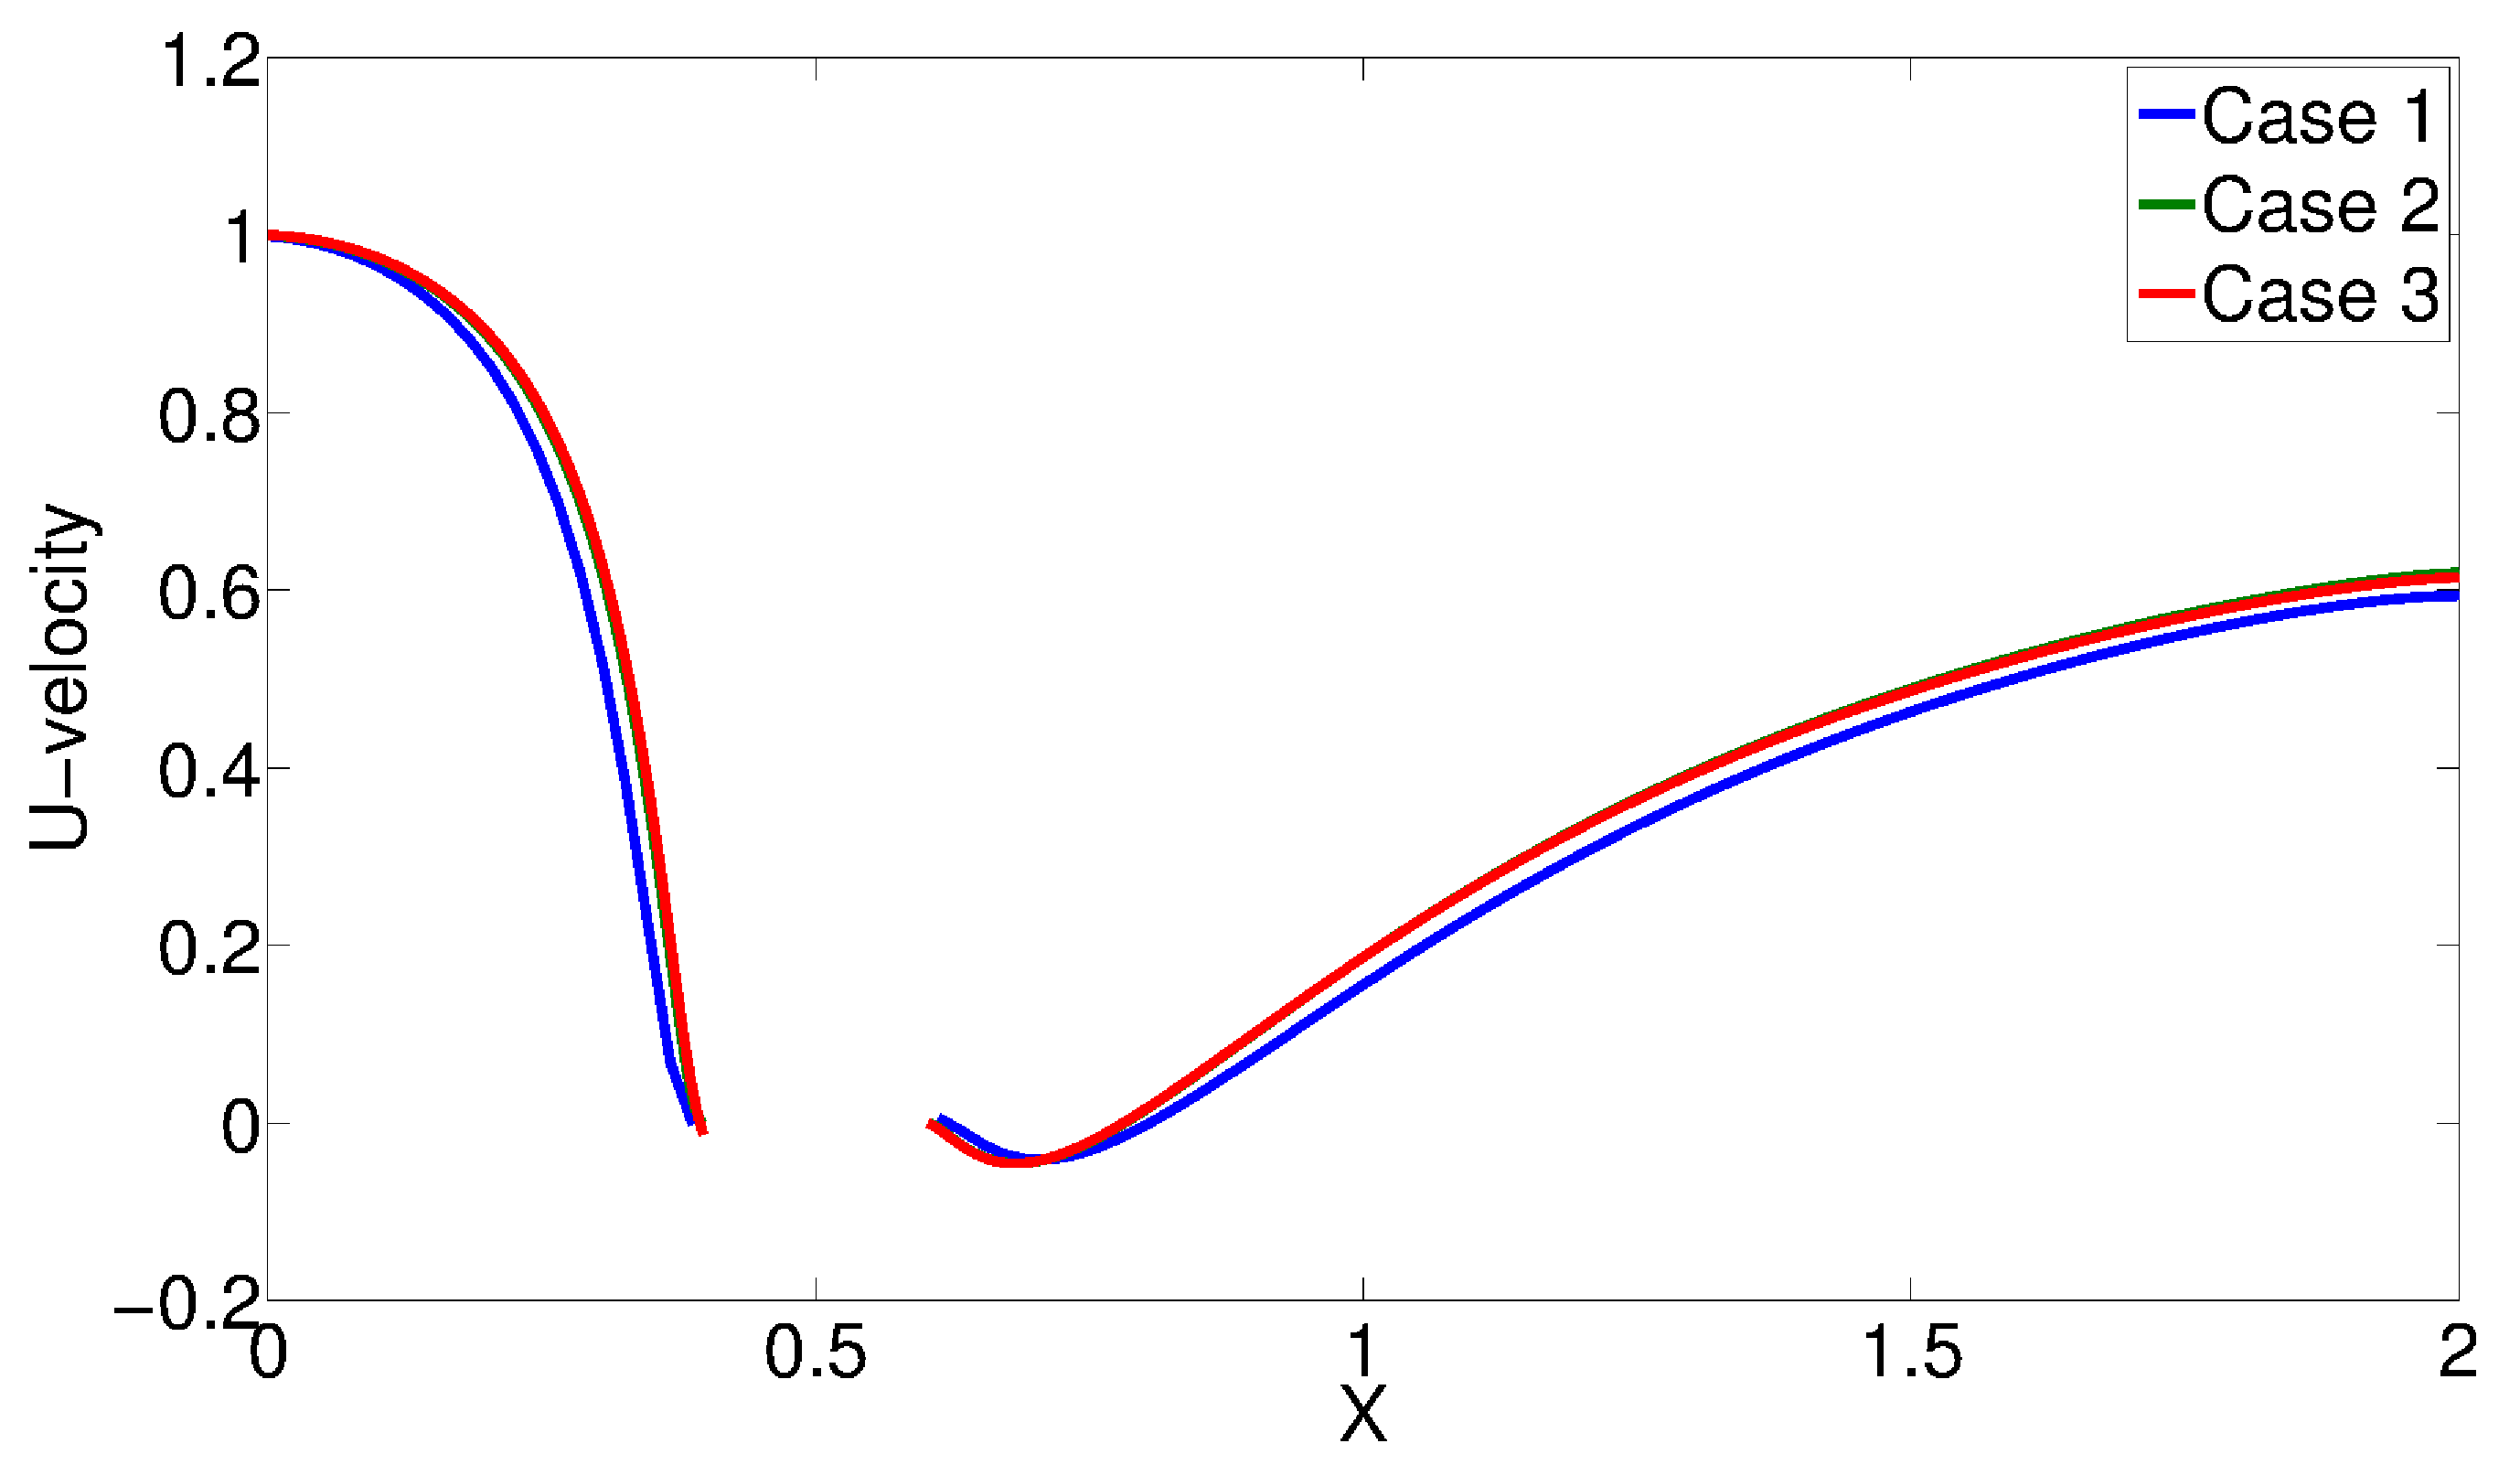
\includegraphics[height=4.0cm]{figure/cylinder/U_convergence_RE100.eps}
	}
	\quad
	\subfigure[U-velocity on $y = 0.5$ for different number of mesh nodes for $Re = 1000$]
	{
	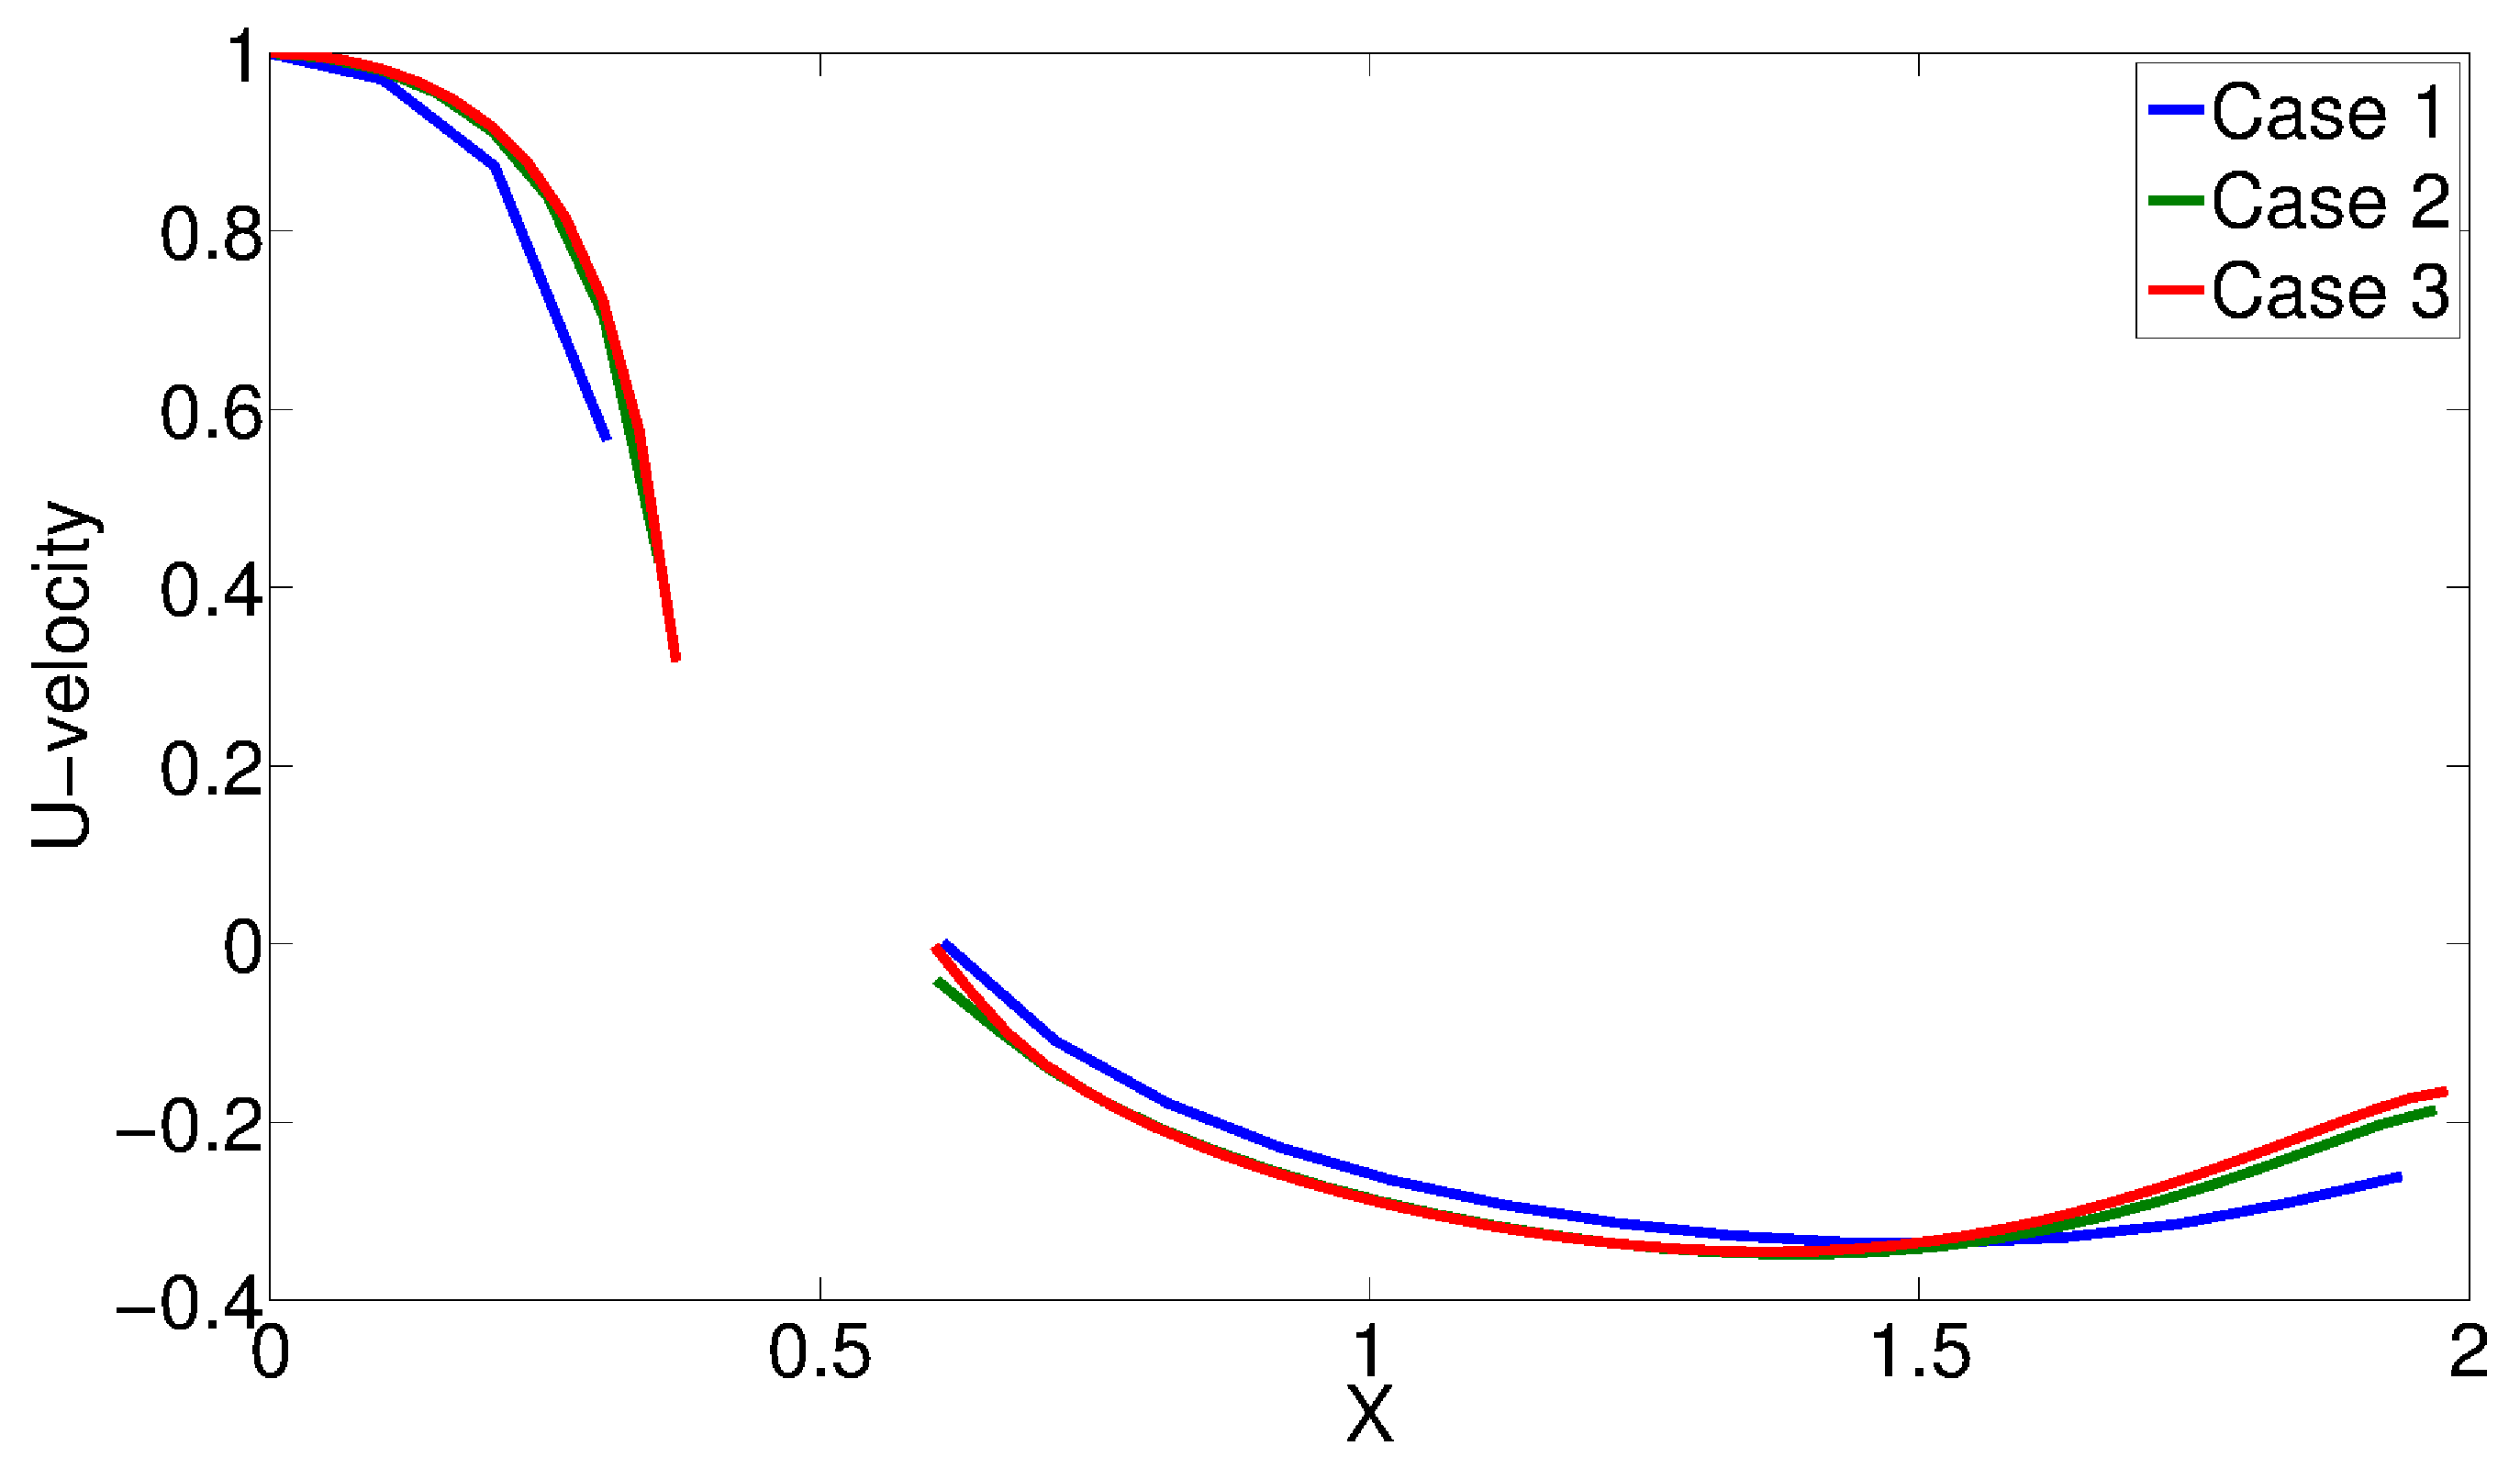
\includegraphics[height=4.0cm]{figure/cylinder/U_convergence_RE1000.eps}
	}
	\\
	\subfigure[V-velocity on $x = 0.25$ for different number of mesh nodes for $Re = 100$]
	{
	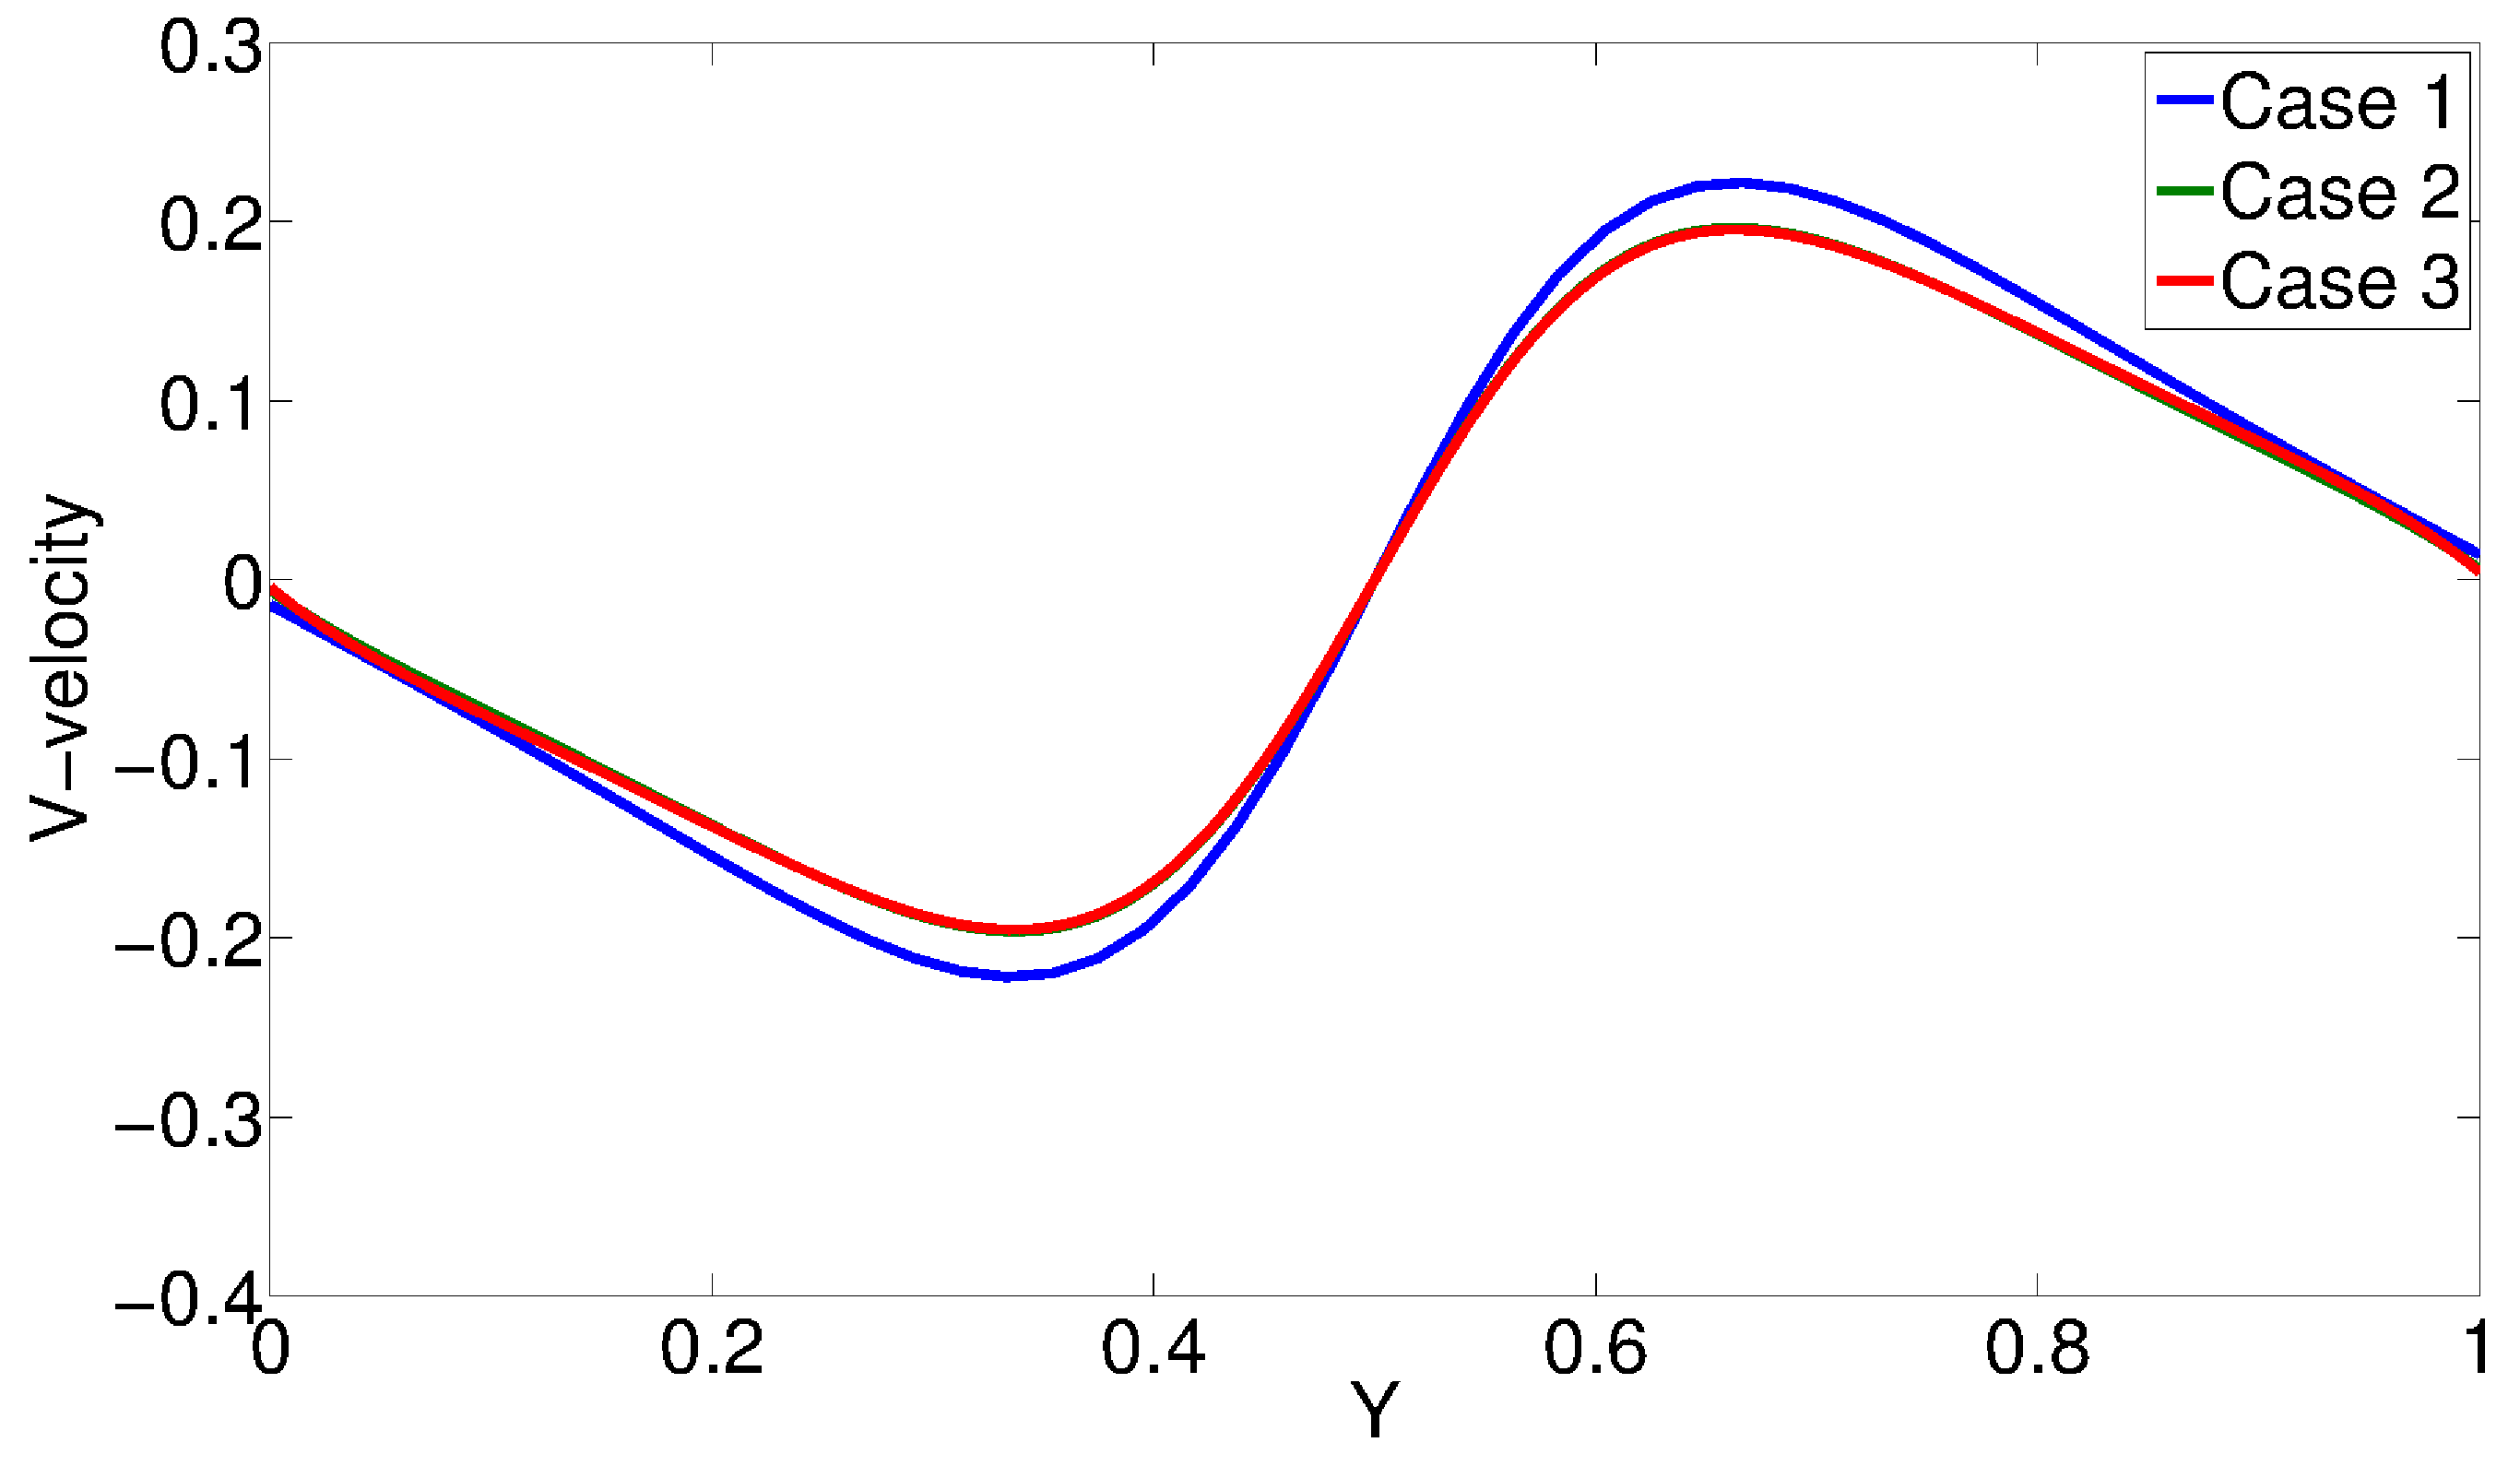
\includegraphics[height=4.0cm]{figure/cylinder/V_convergence_RE100.eps}
	}
	\quad
	\subfigure[V-velocity on $x = 0.25$ for different number of mesh nodes for $Re = 1000$]
	{
	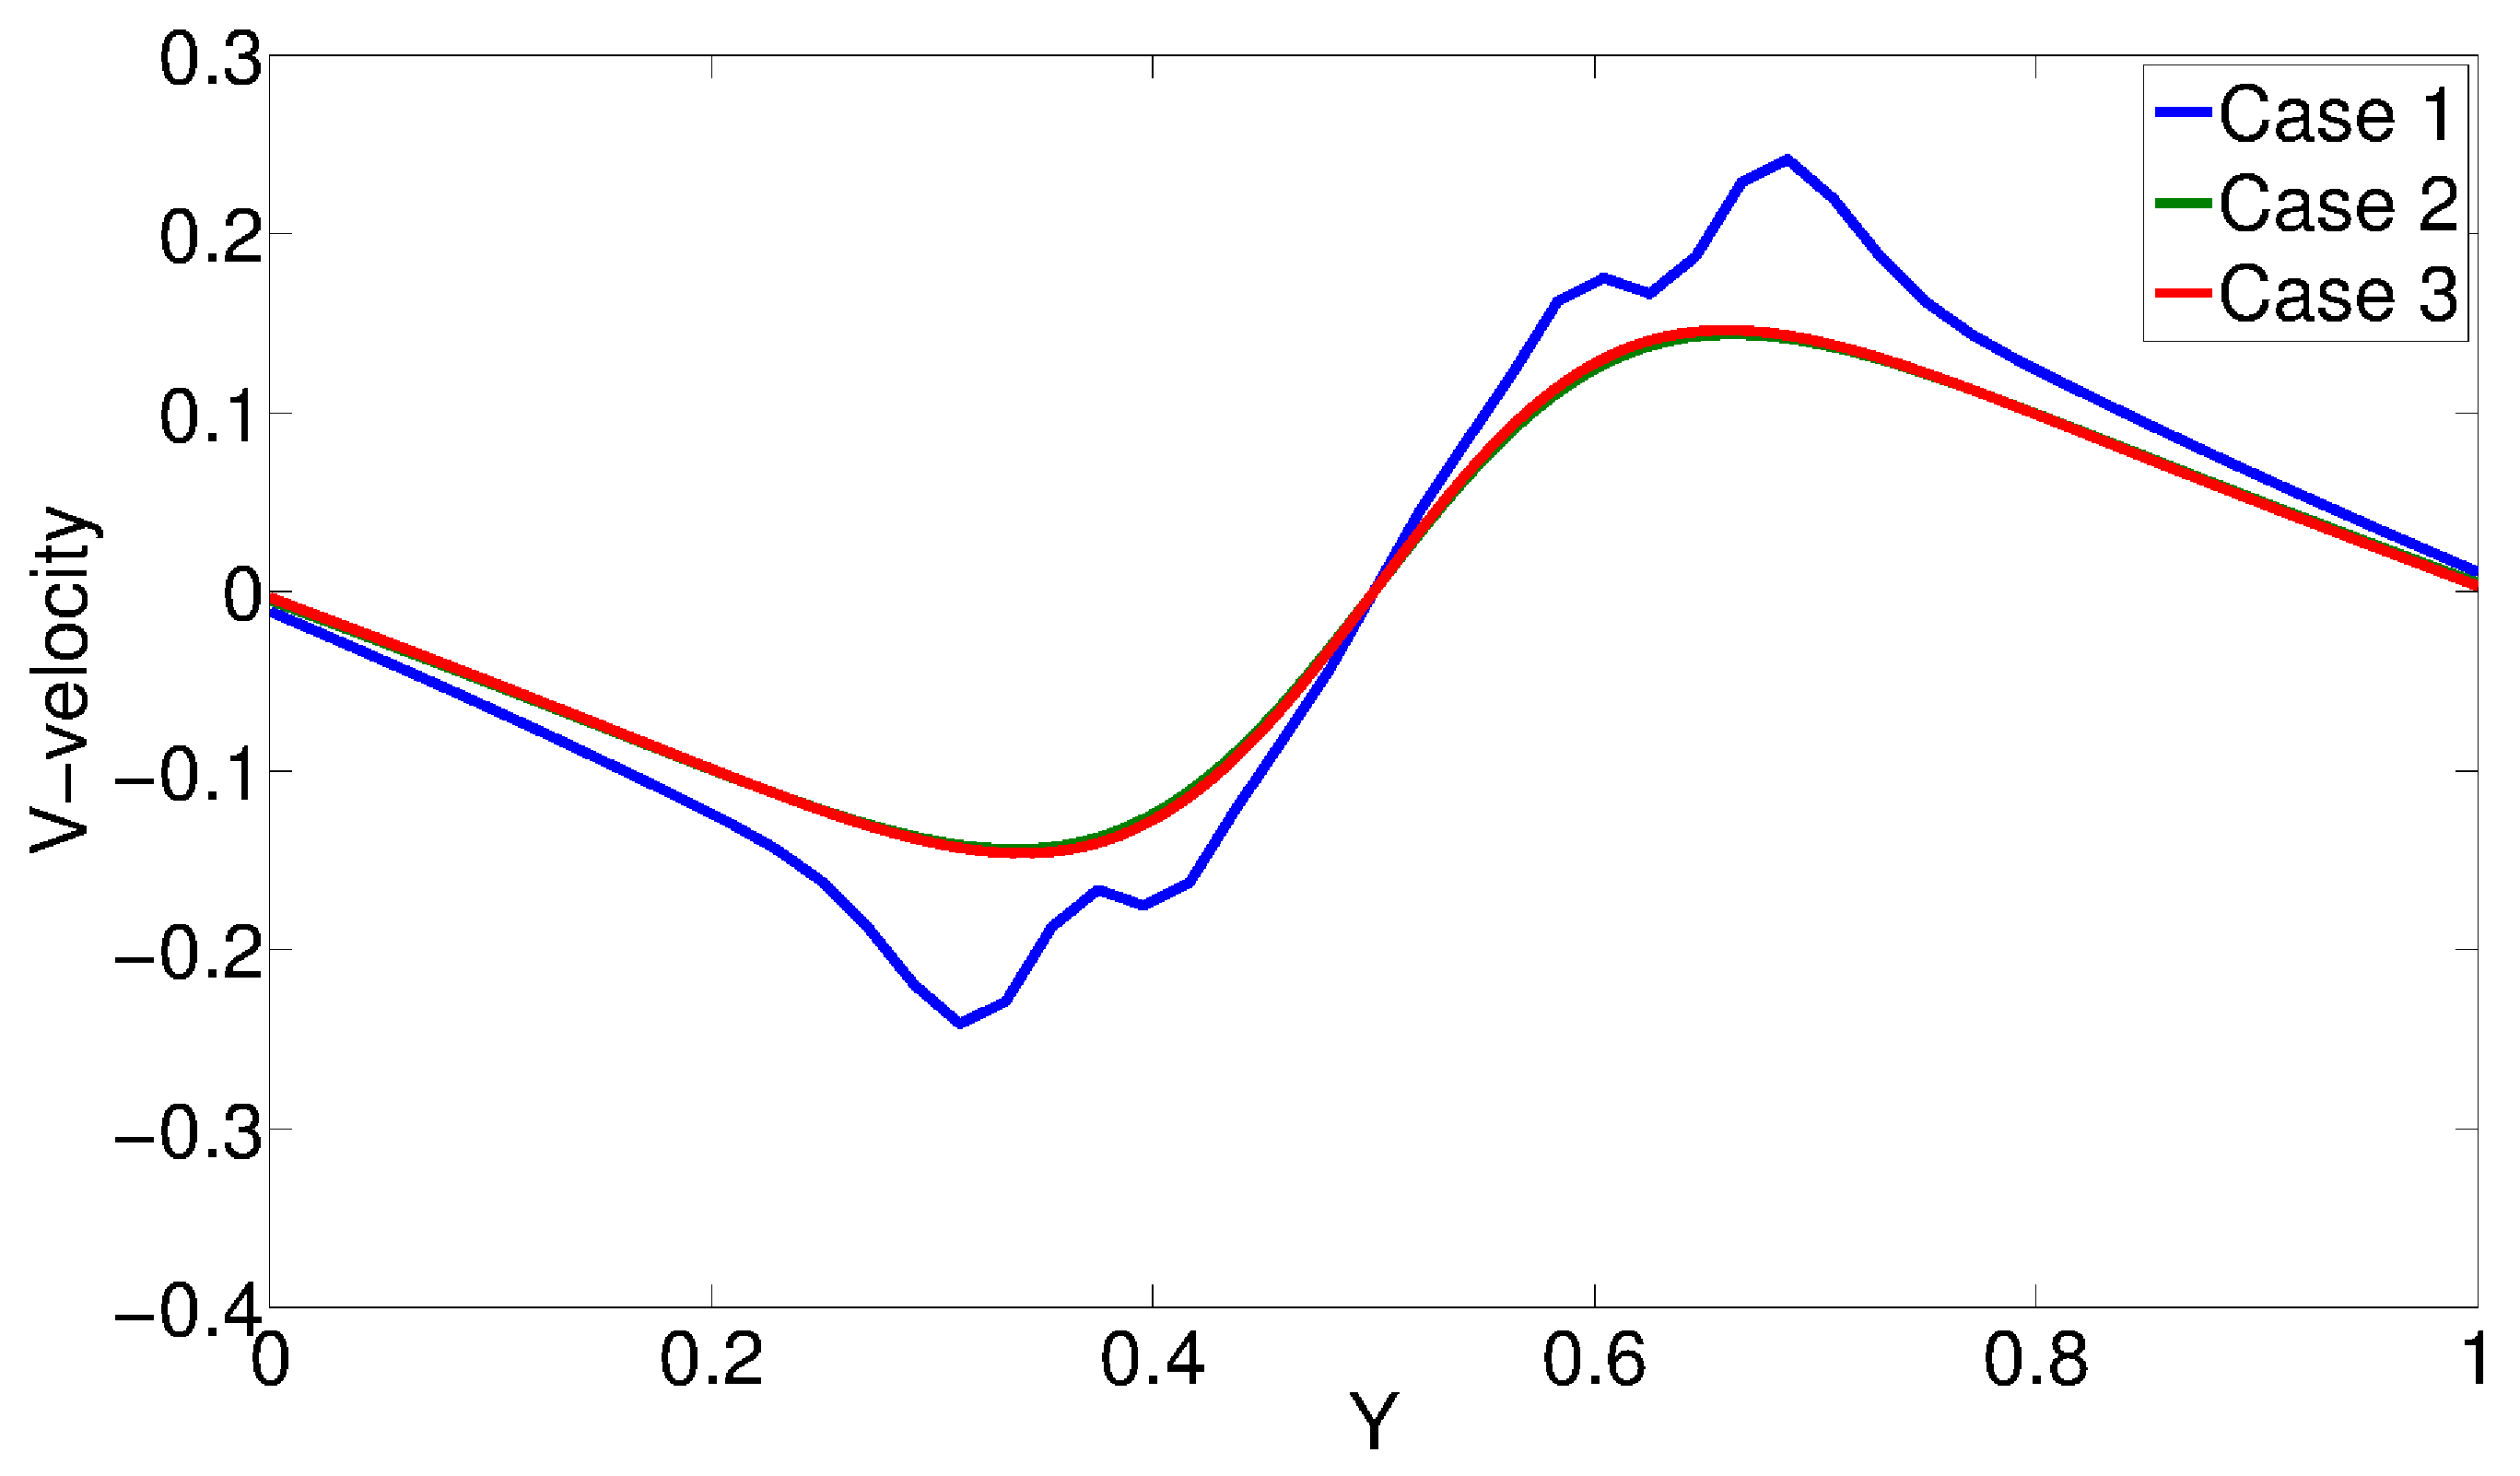
\includegraphics[height=4.0cm]{figure/cylinder/V_convergence_RE1000.eps}
	}
	\caption{Results of convergence study for flow over cylinder. Case 1, case 2, and case 3 are domains with $100 \times 50$, $200 \times 100$, $300 \times 150$ nodes.}
	\label{fig:convegence_study}
\end{figure}
%

The time history of force terms of the surface of the cylinder are shown in Figure \ref{fig:cylinderForceTerms}. We choose five probe locations of the surface of the cylinder to track the force values. It should be noted that these are the force terms added to the Navier-Stokes equations to represent the boundary not the forces acting of the surface of the cylinder due to hydrodynamic pressure. As shown in Figure \ref{fig:cylinderForceTerms}, the values of the forcing function starts oscillating at the beginning and reaches a steady-state value after sometime. This indicates that we reached a steady-state solution.

%
\begin{figure}[H]
	\centering
	\subfigure[Forcing term in $x$ direction.]
	{
	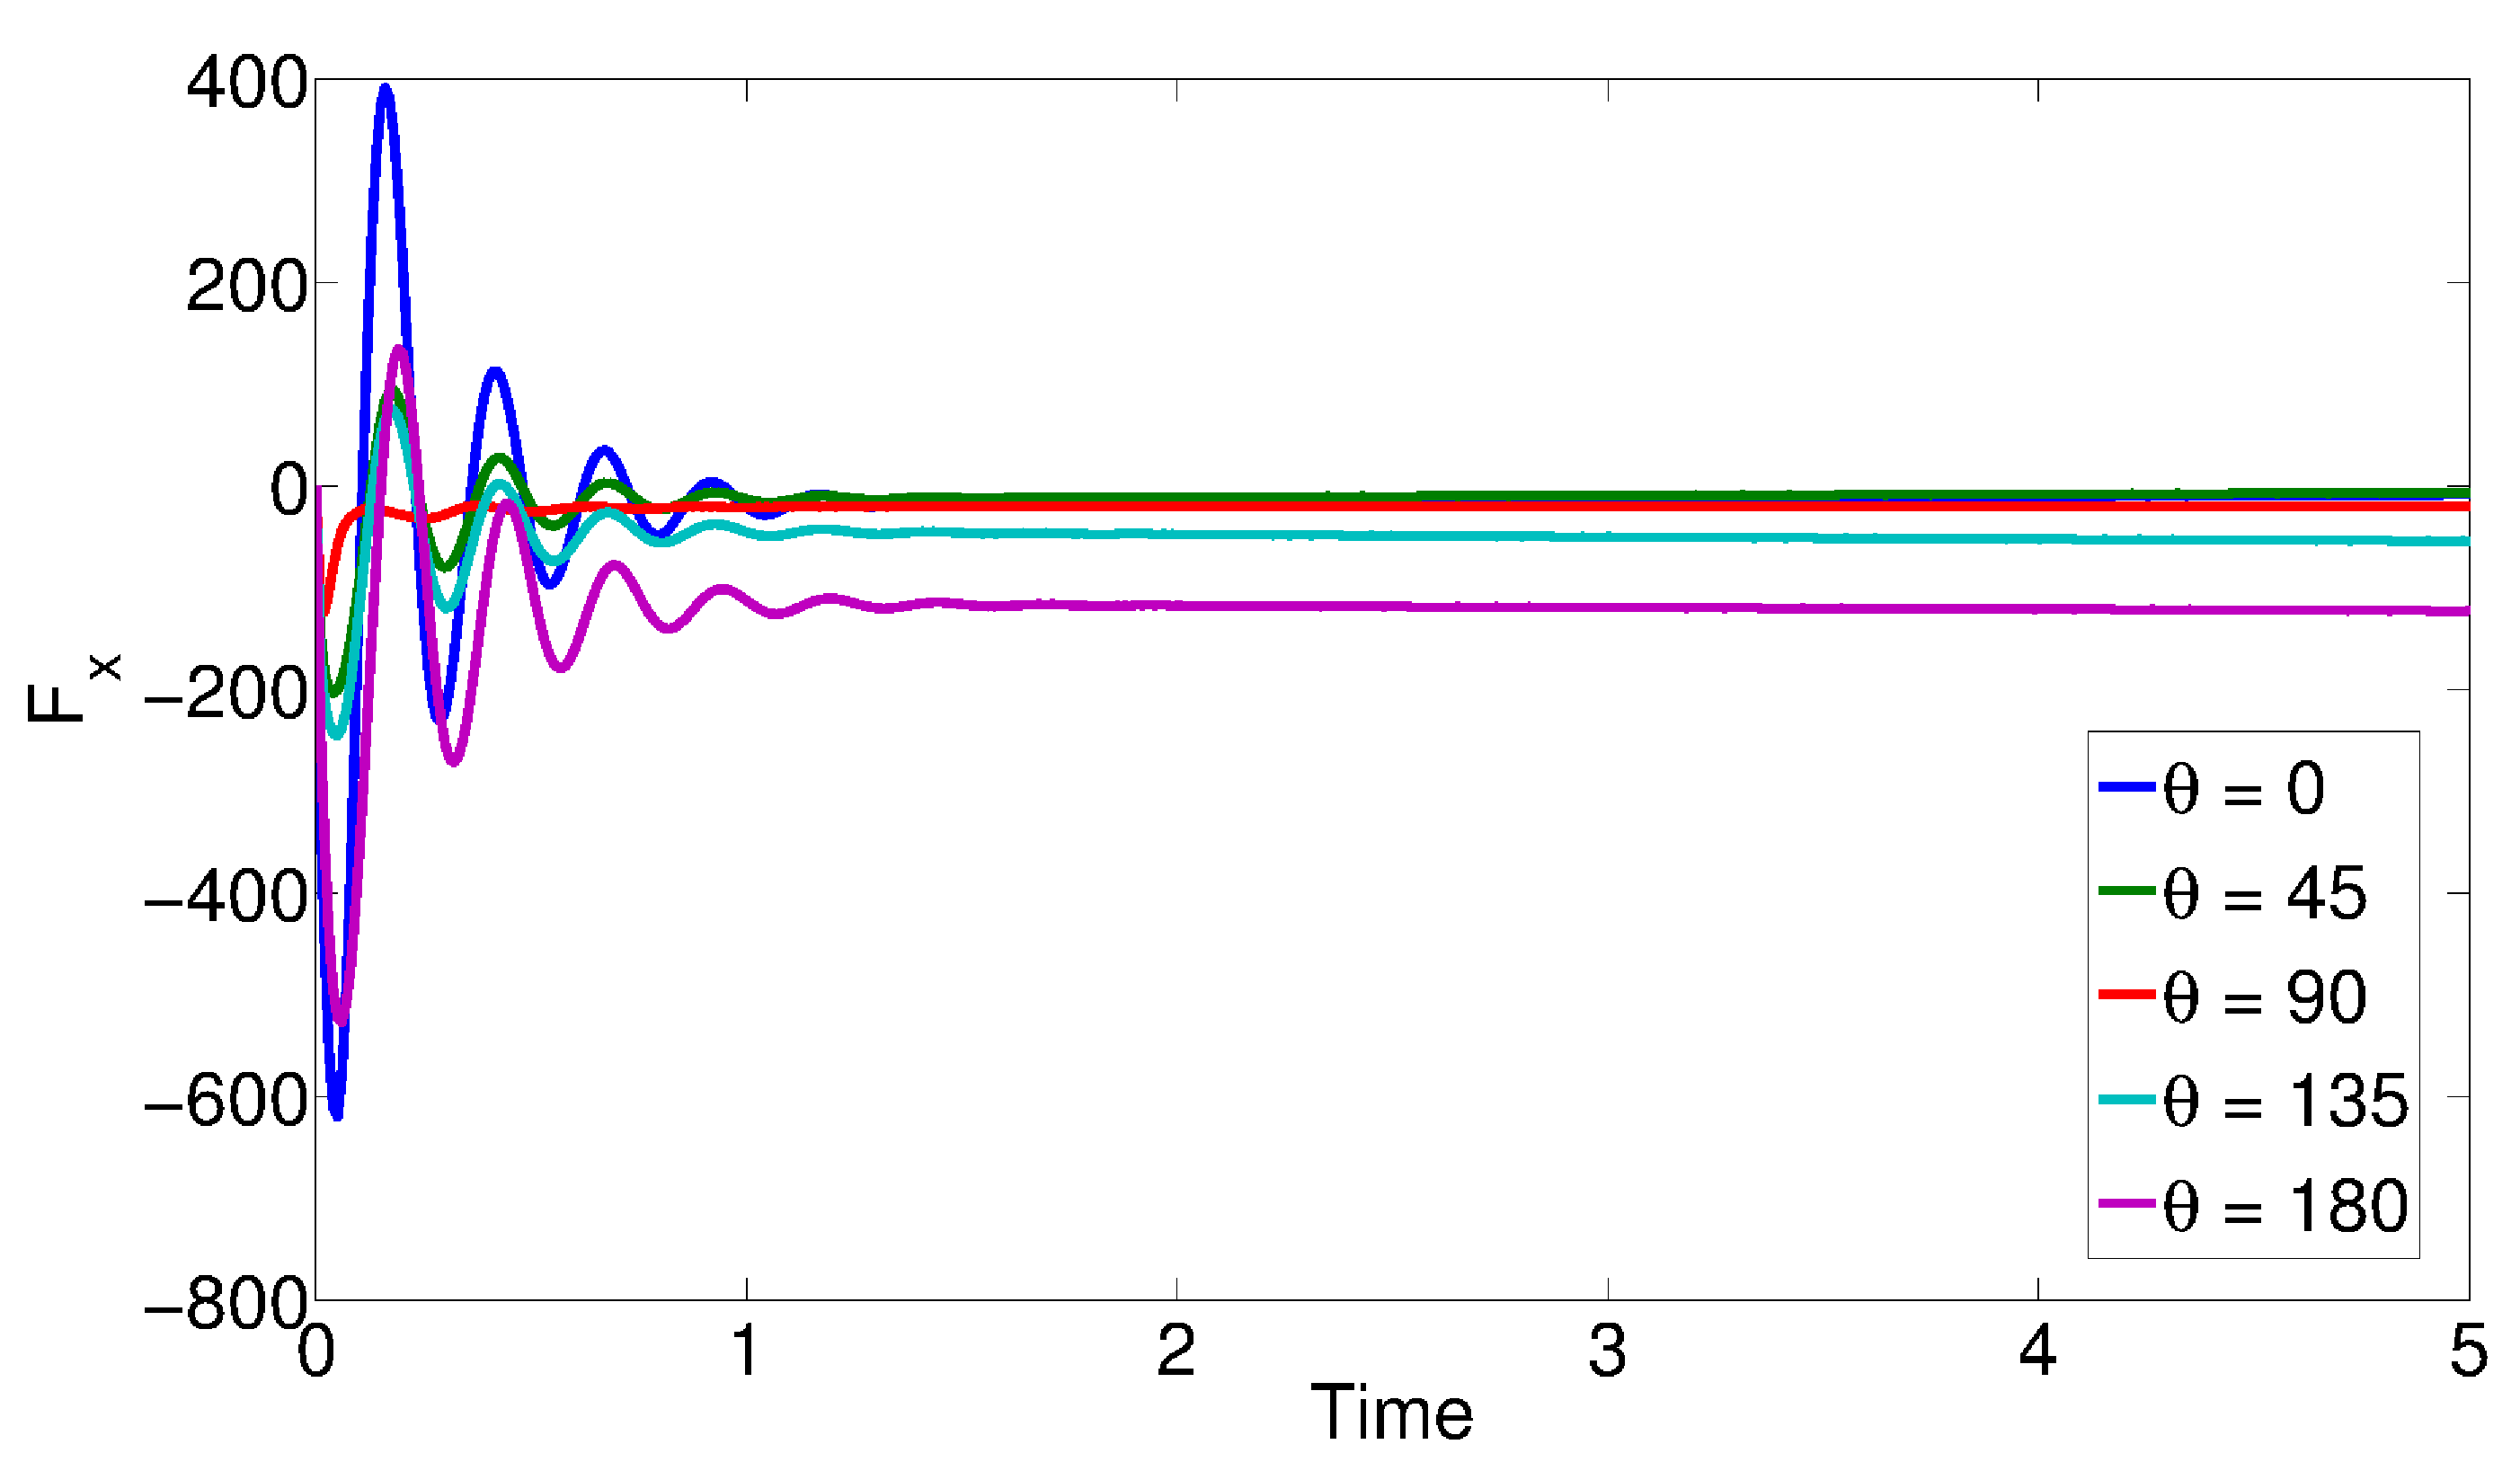
\includegraphics[height=4.5cm]{figure/cylinder/fx.eps}
	}
	\quad
	\subfigure[Forcing term in $y$ direction.]
	{
	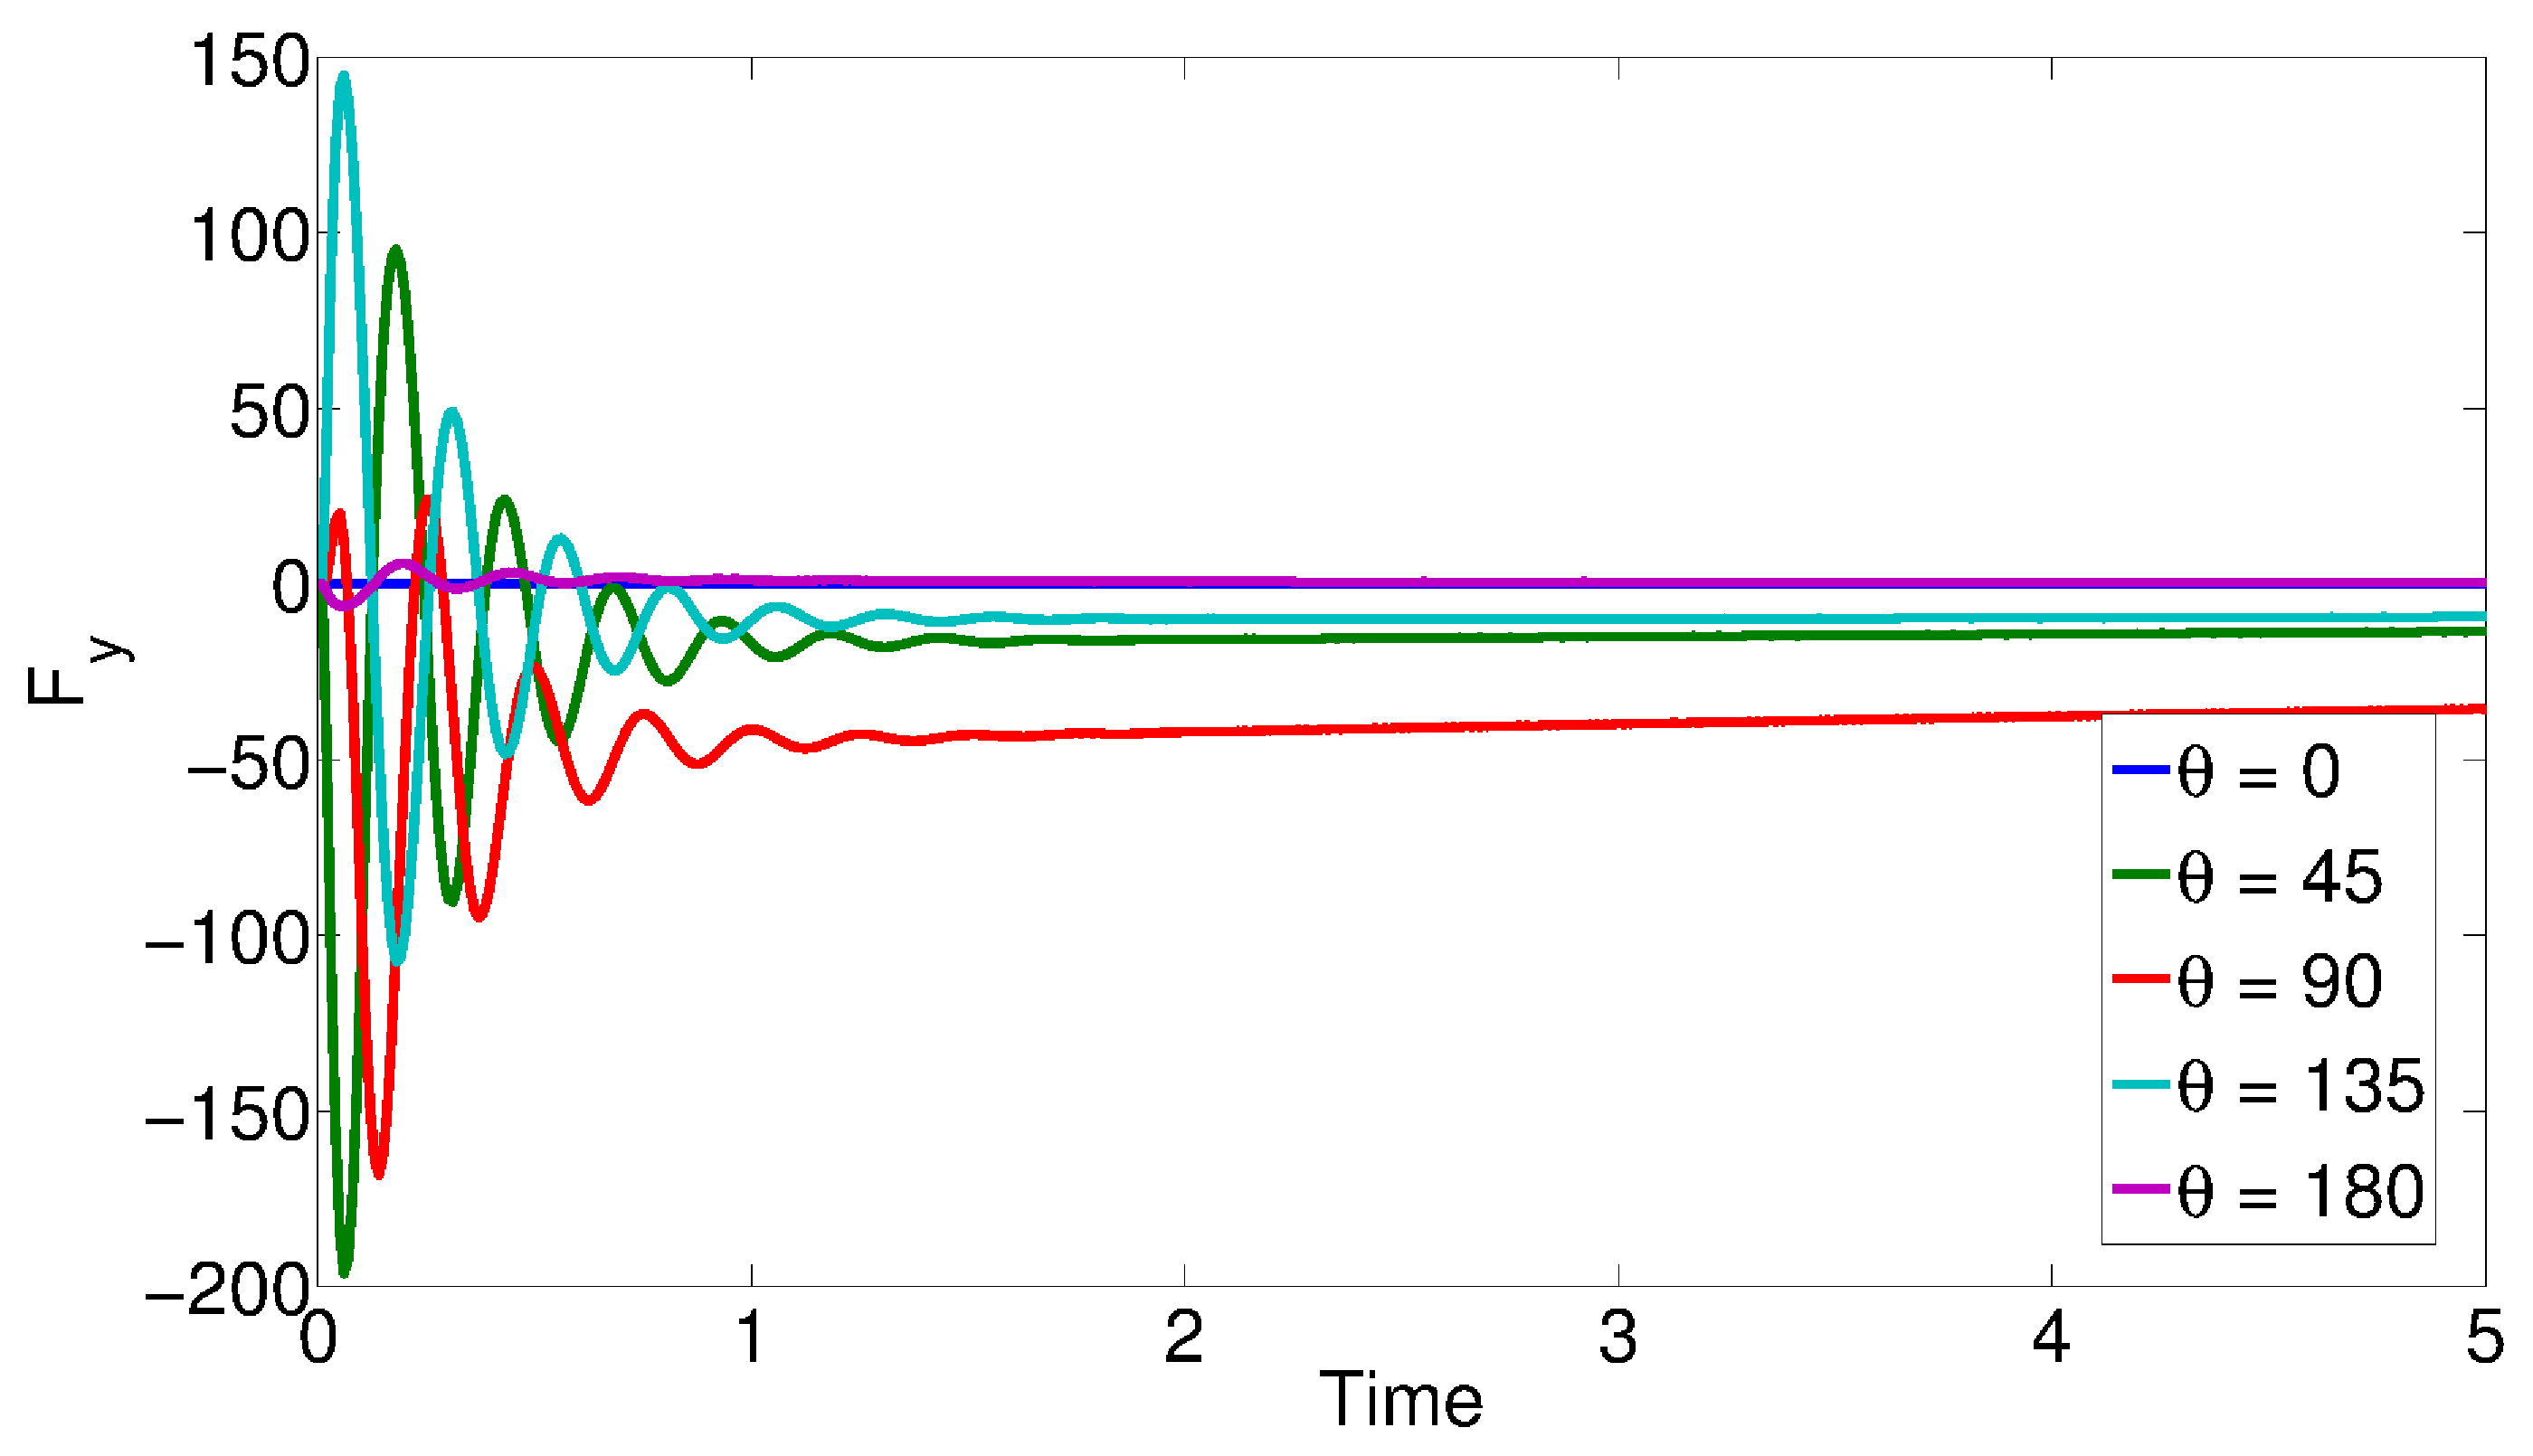
\includegraphics[height=4.5cm]{figure/cylinder/fy.eps}
	}
	\caption{Forcing terms on the surface of the cylinder. $\theta = 0$ is on the front and $\theta = 180$ is on the back of the cylinder for Re = 100.}
	\label{fig:cylinderForceTerms}
\end{figure}
%

The sensitivity contour plots for the pressure and velocity for different values of Reynolds number are shown in Figures \ref{fig:cylinderSensitivityContourRE100} and \ref{fig:cylinderSensitivityContourRE1000}. As shown here, the contour plots for the continuum sensitivity analysis and complex step results agrees well with each other.

%
\begin{figure}[H]
	\centering
	\subfigure[Continuum sensitivity result for pressure sensitivity]
	{
	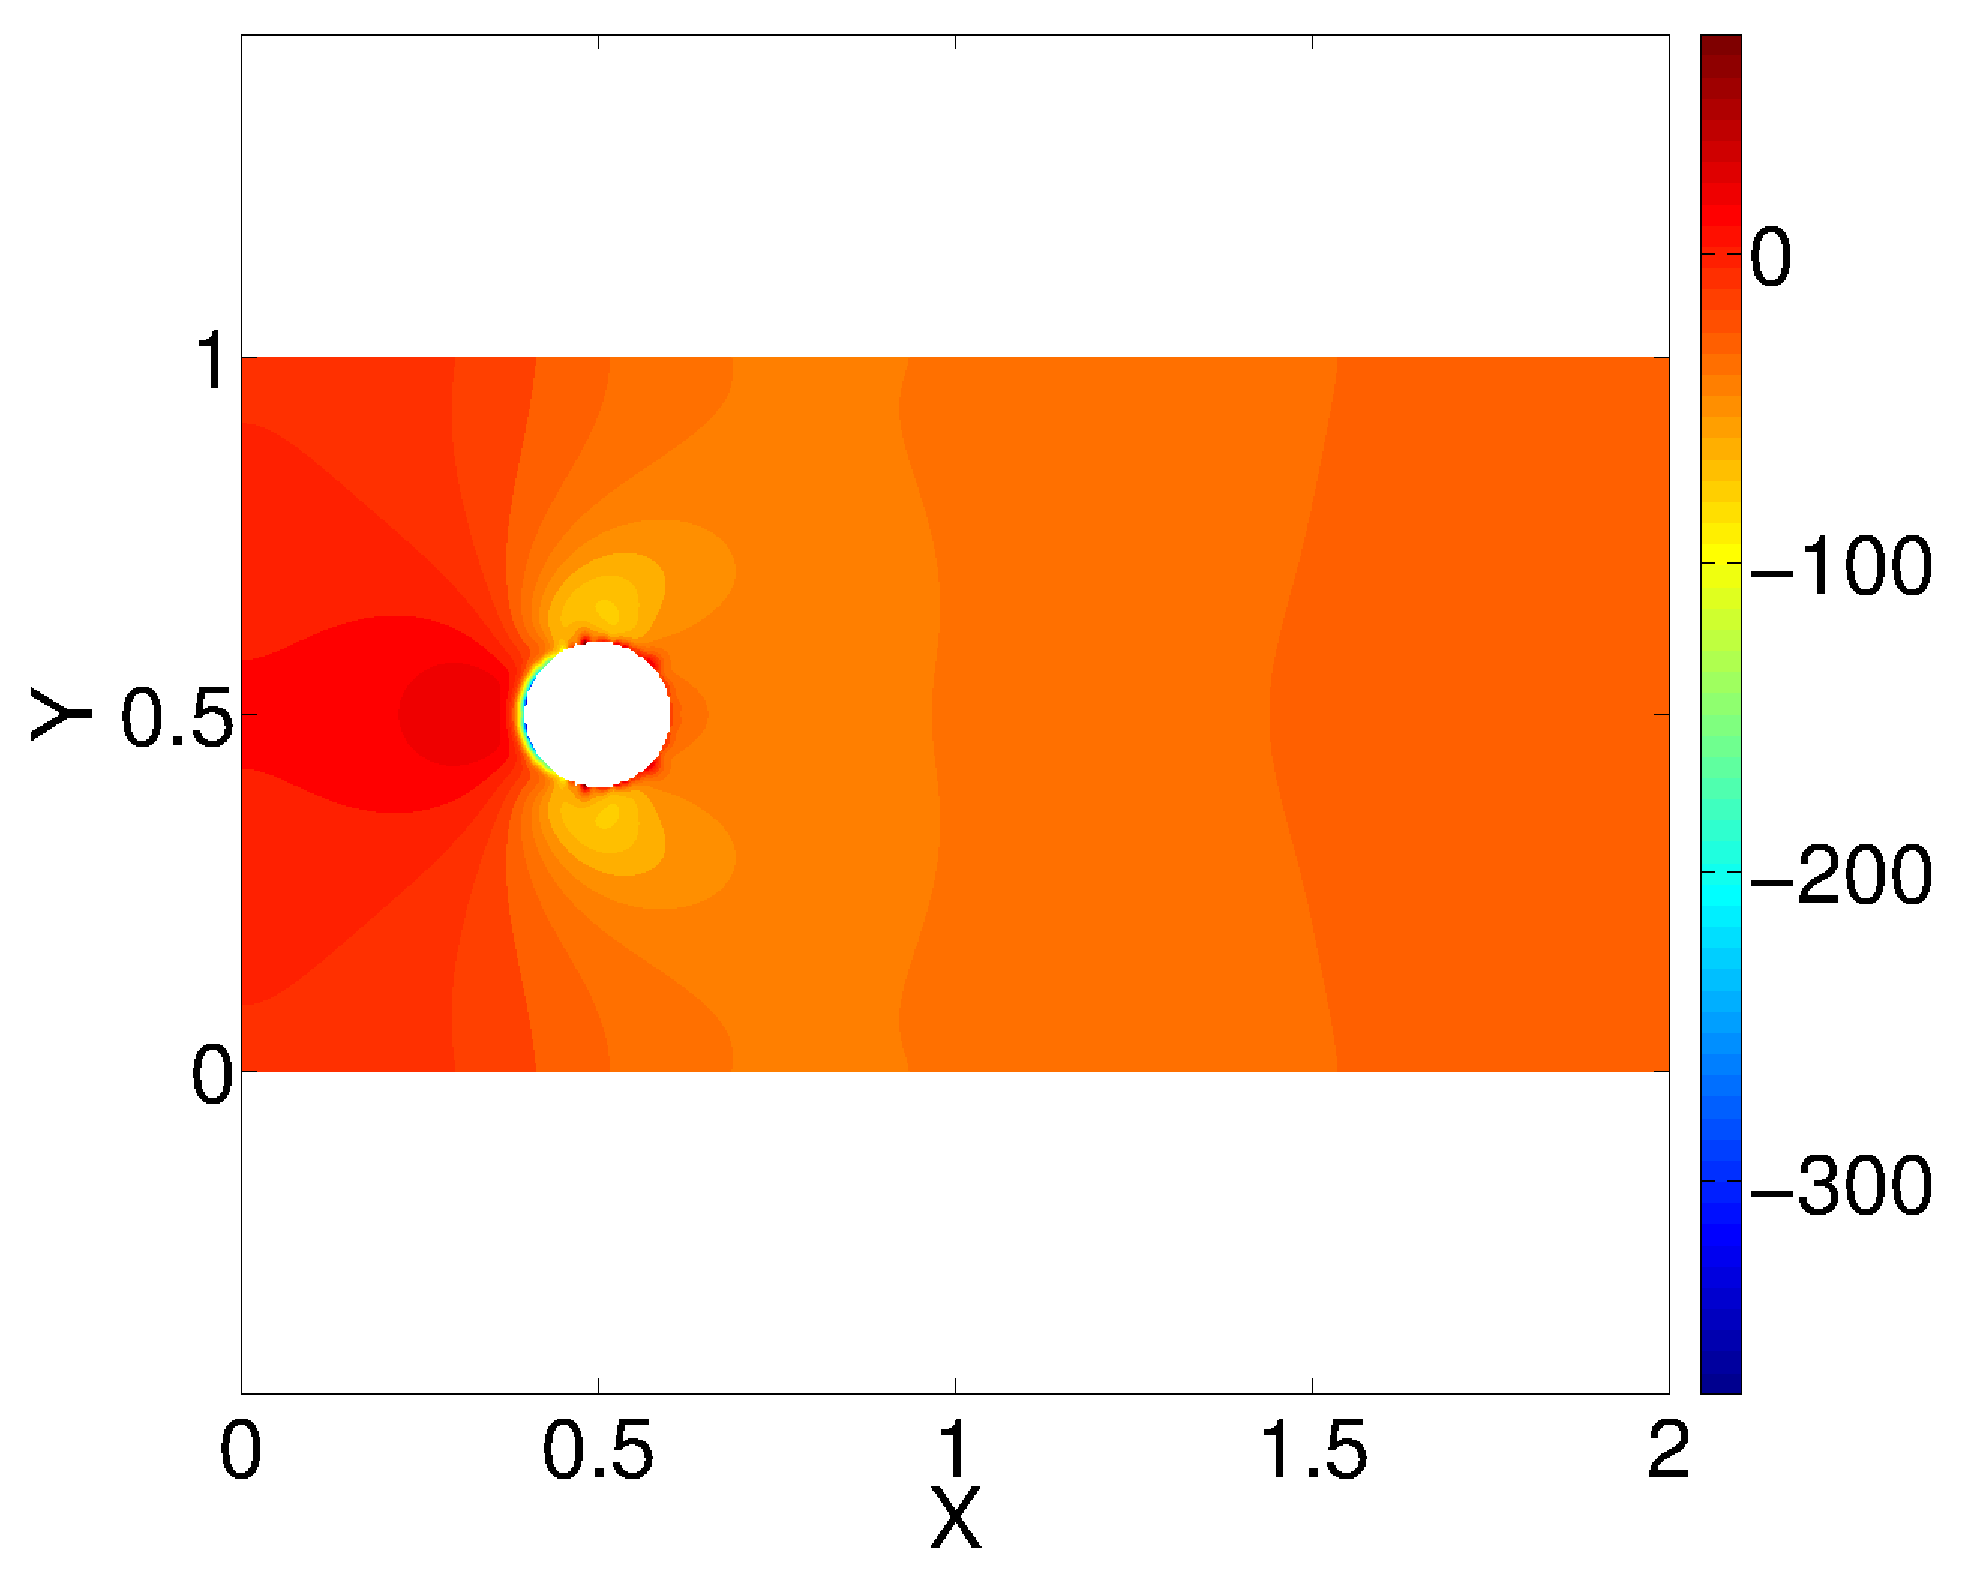
\includegraphics[height=6.0cm]{figure/cylinder/Pp_RE100.eps}
	}
	\quad
	\subfigure[Complex step result for pressure sensitivity]
	{
	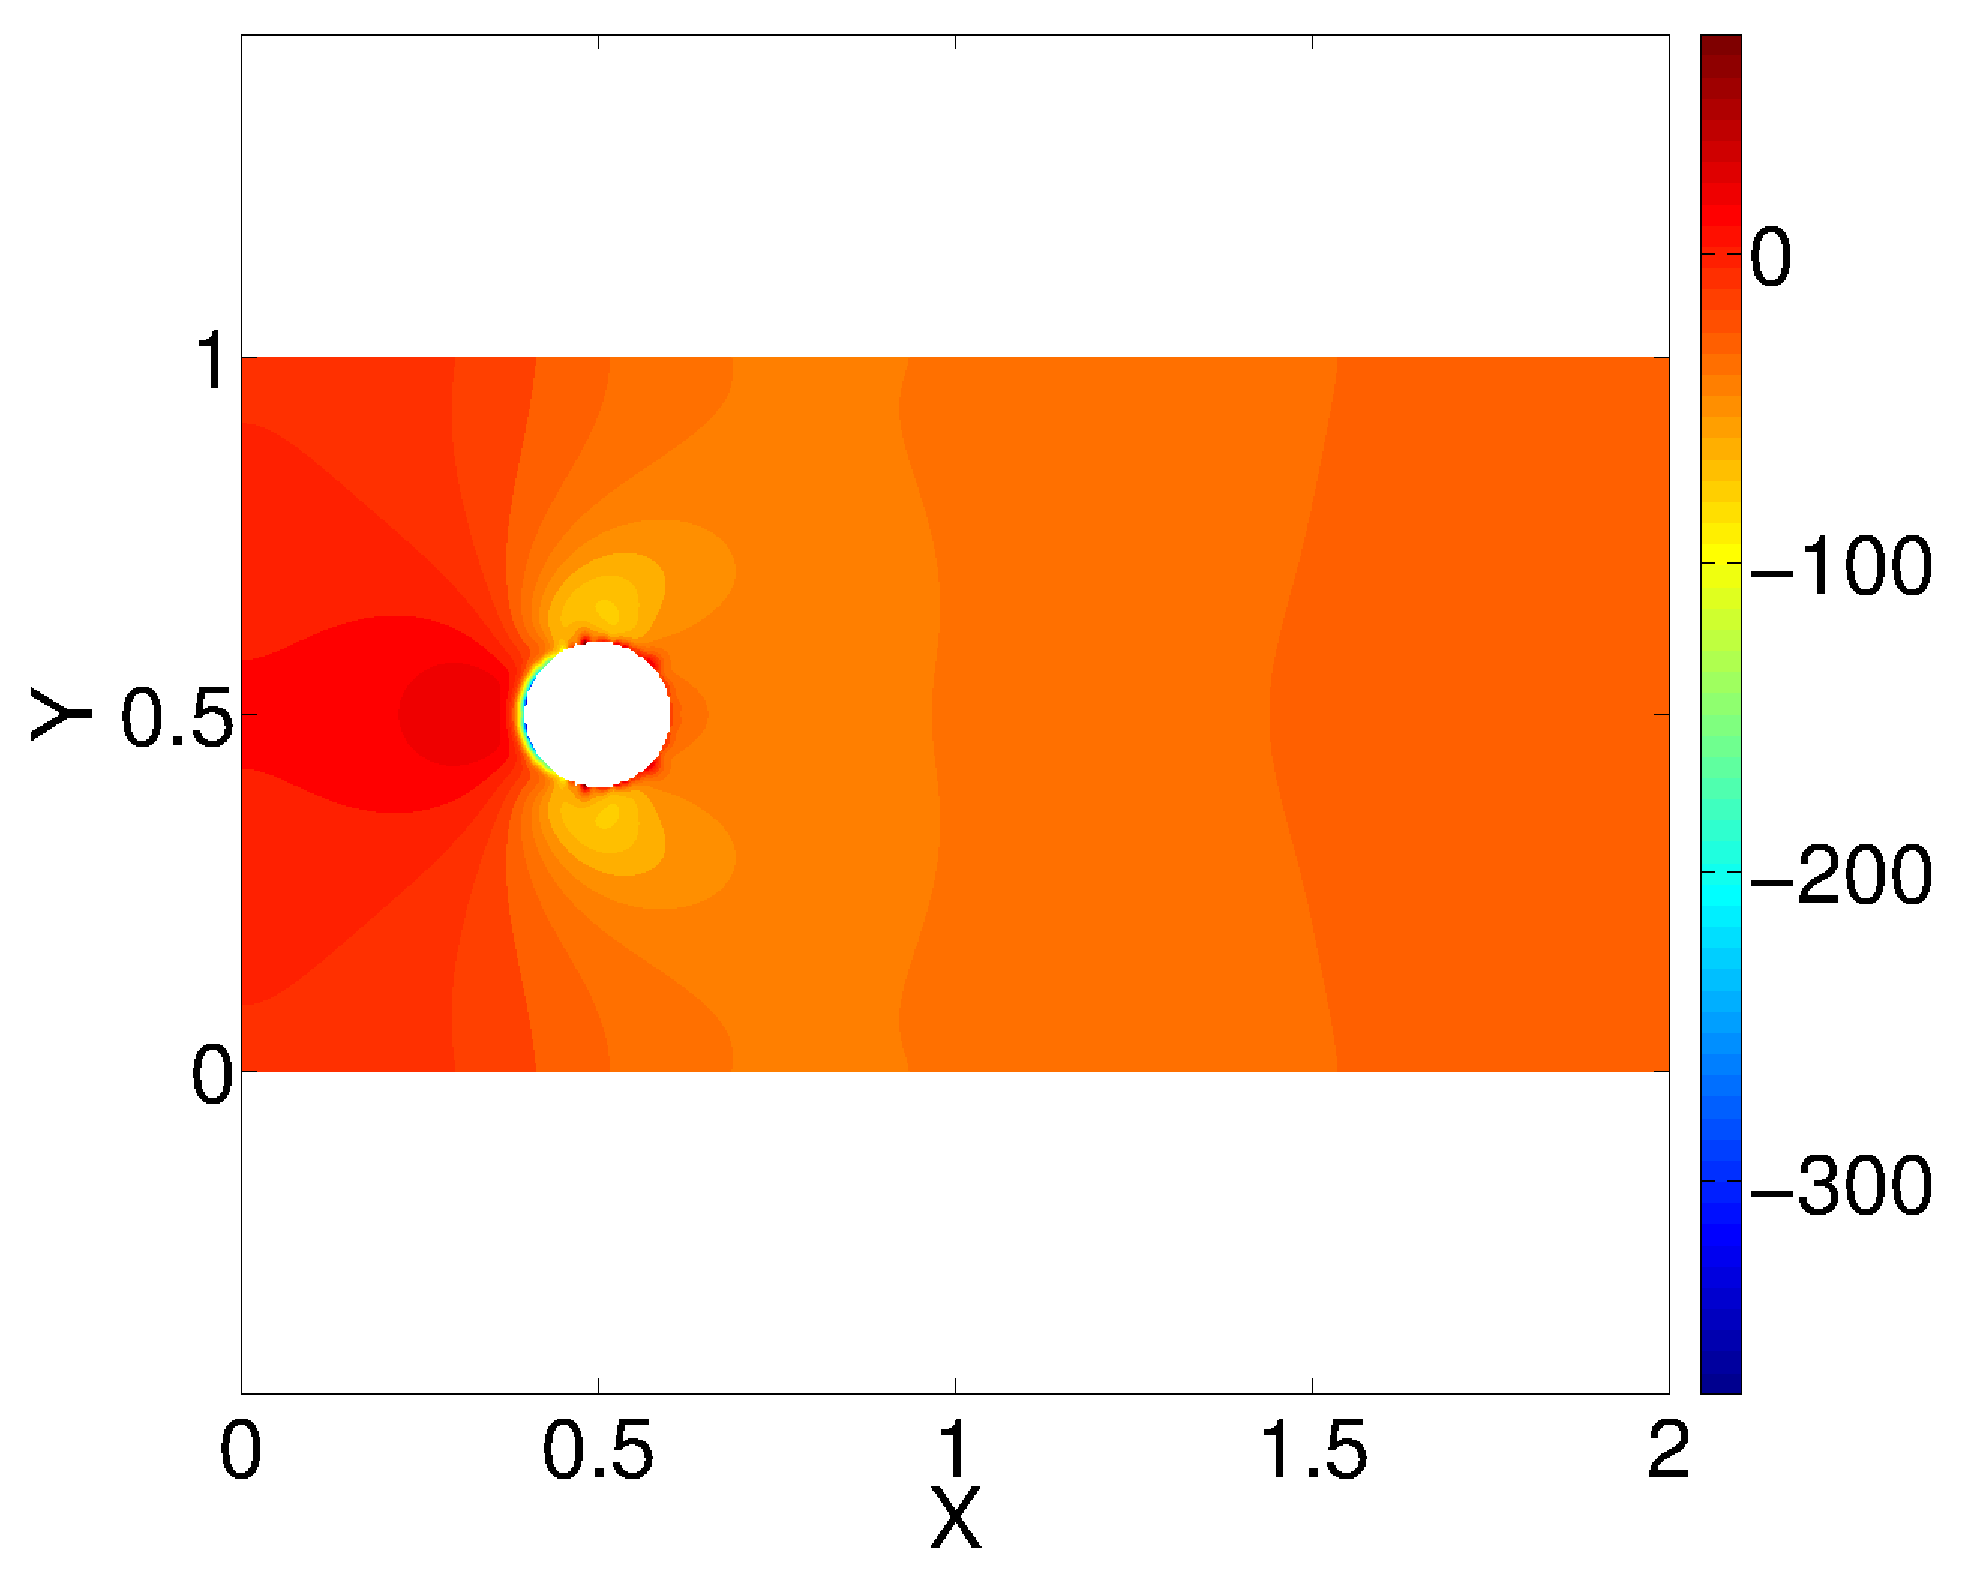
\includegraphics[height=6.0cm]{figure/cylinder/Pp_RE100.eps}
	}
	\\
	\subfigure[Continuum sensitivity result for u-velocity sensitivity]
	{
	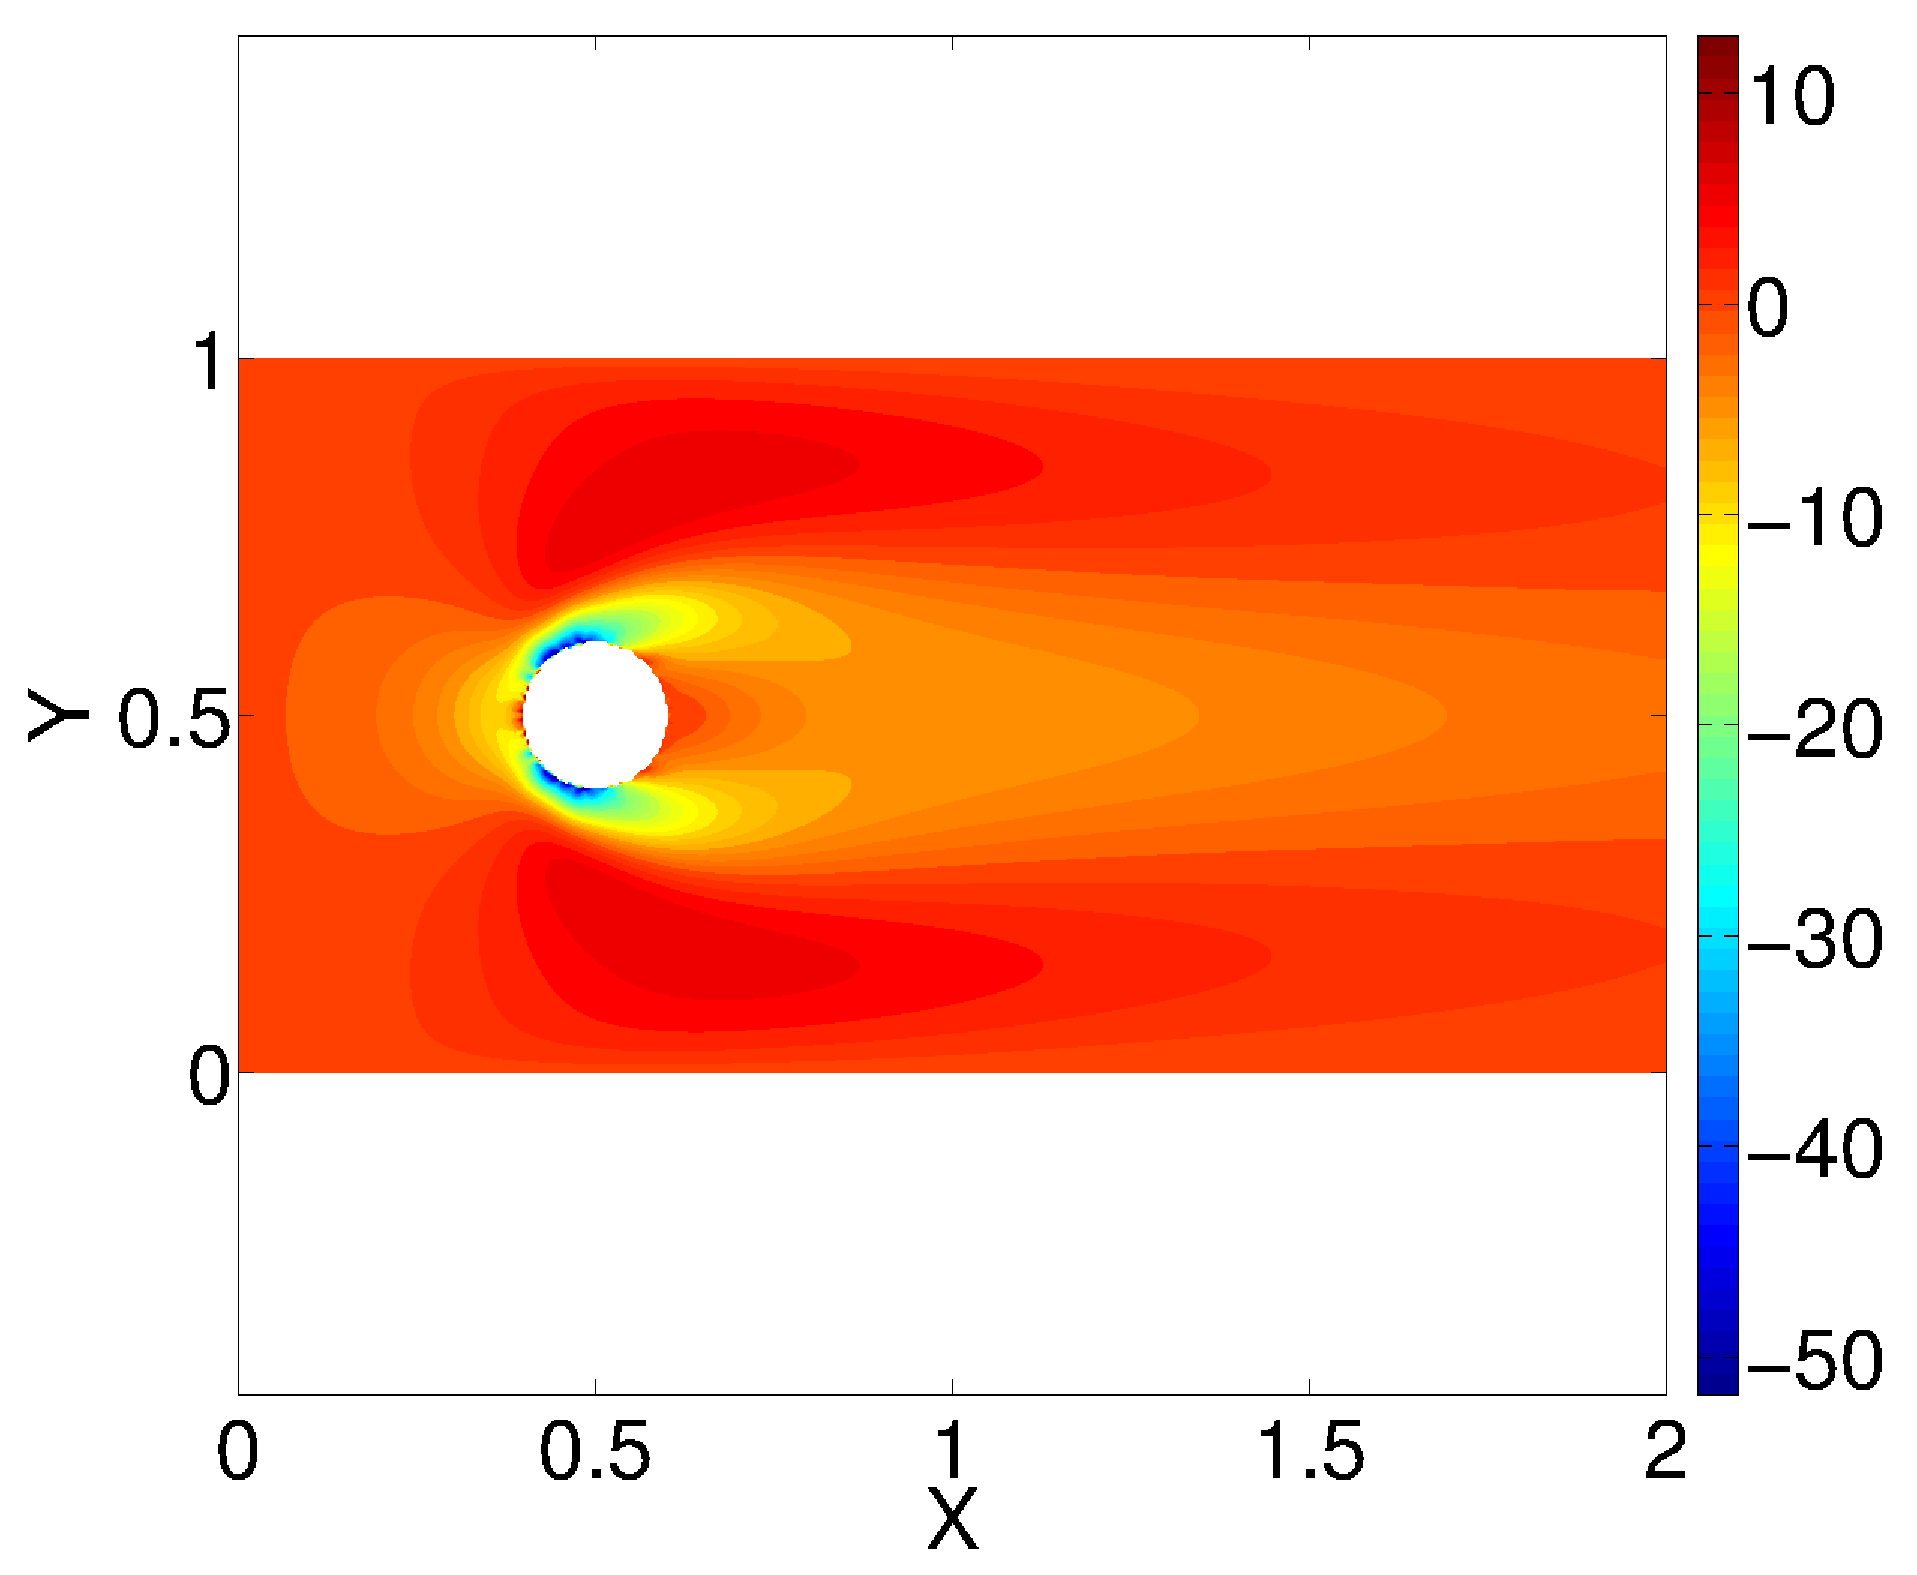
\includegraphics[height=6.0cm]{figure/cylinder/Up_RE100.eps}
	}
	\quad
	\subfigure[Complex step result for u-velocity sensitivity]
	{
	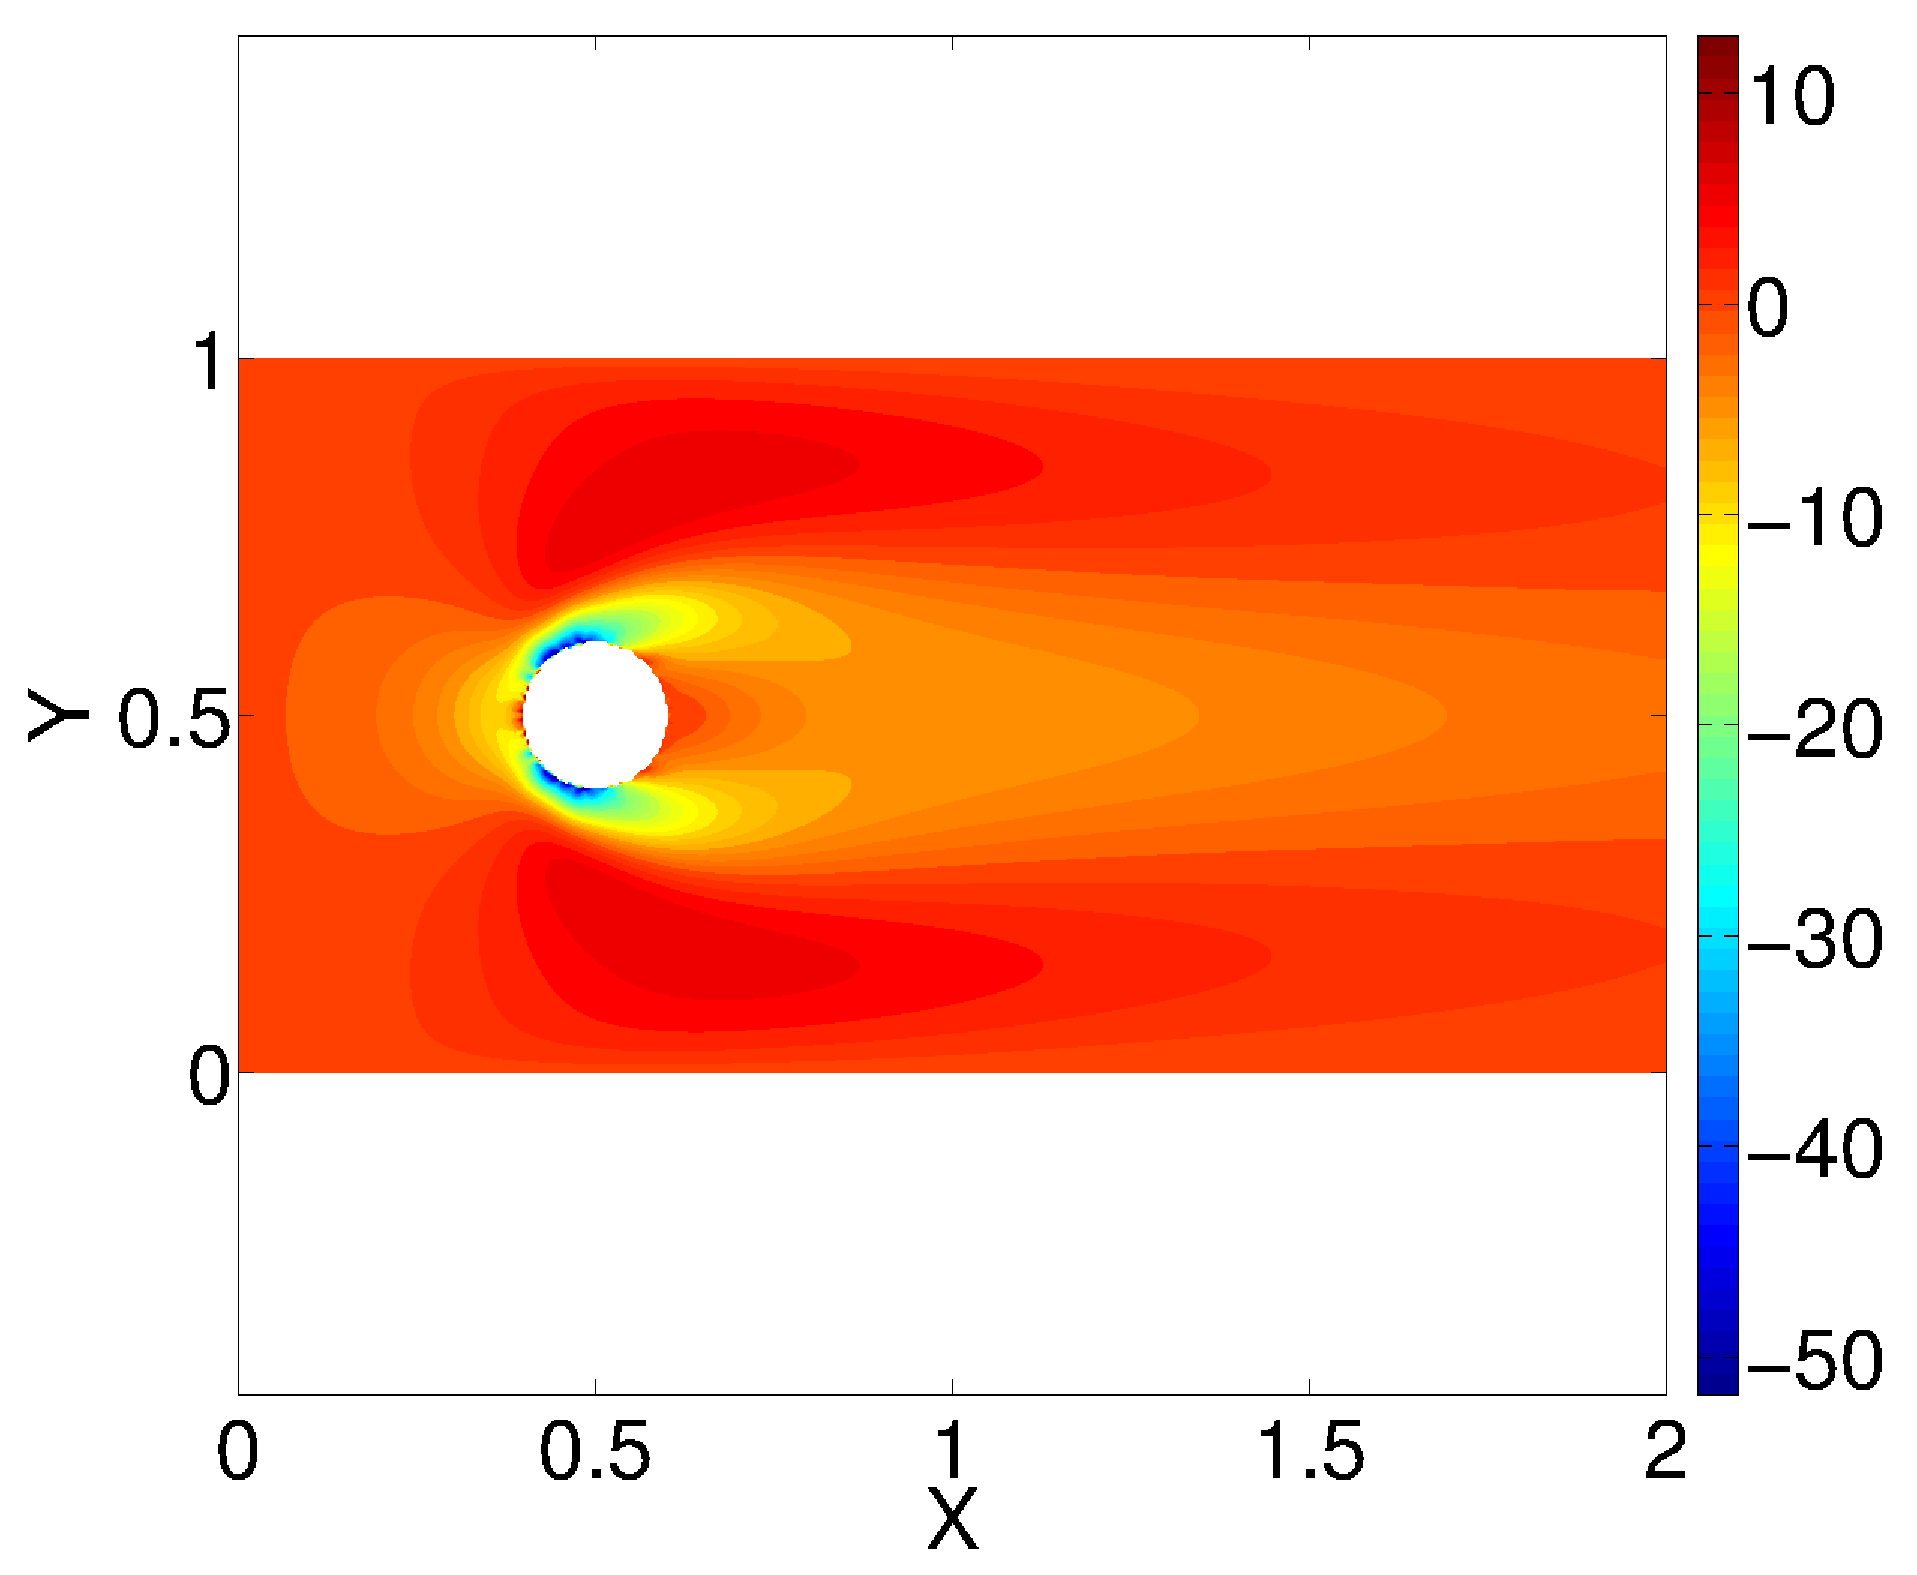
\includegraphics[height=6.0cm]{figure/cylinder/Up_RE100.eps}
	}
	\\
	\subfigure[Continuum sensitivity result for v-velocity sensitivity]
	{
	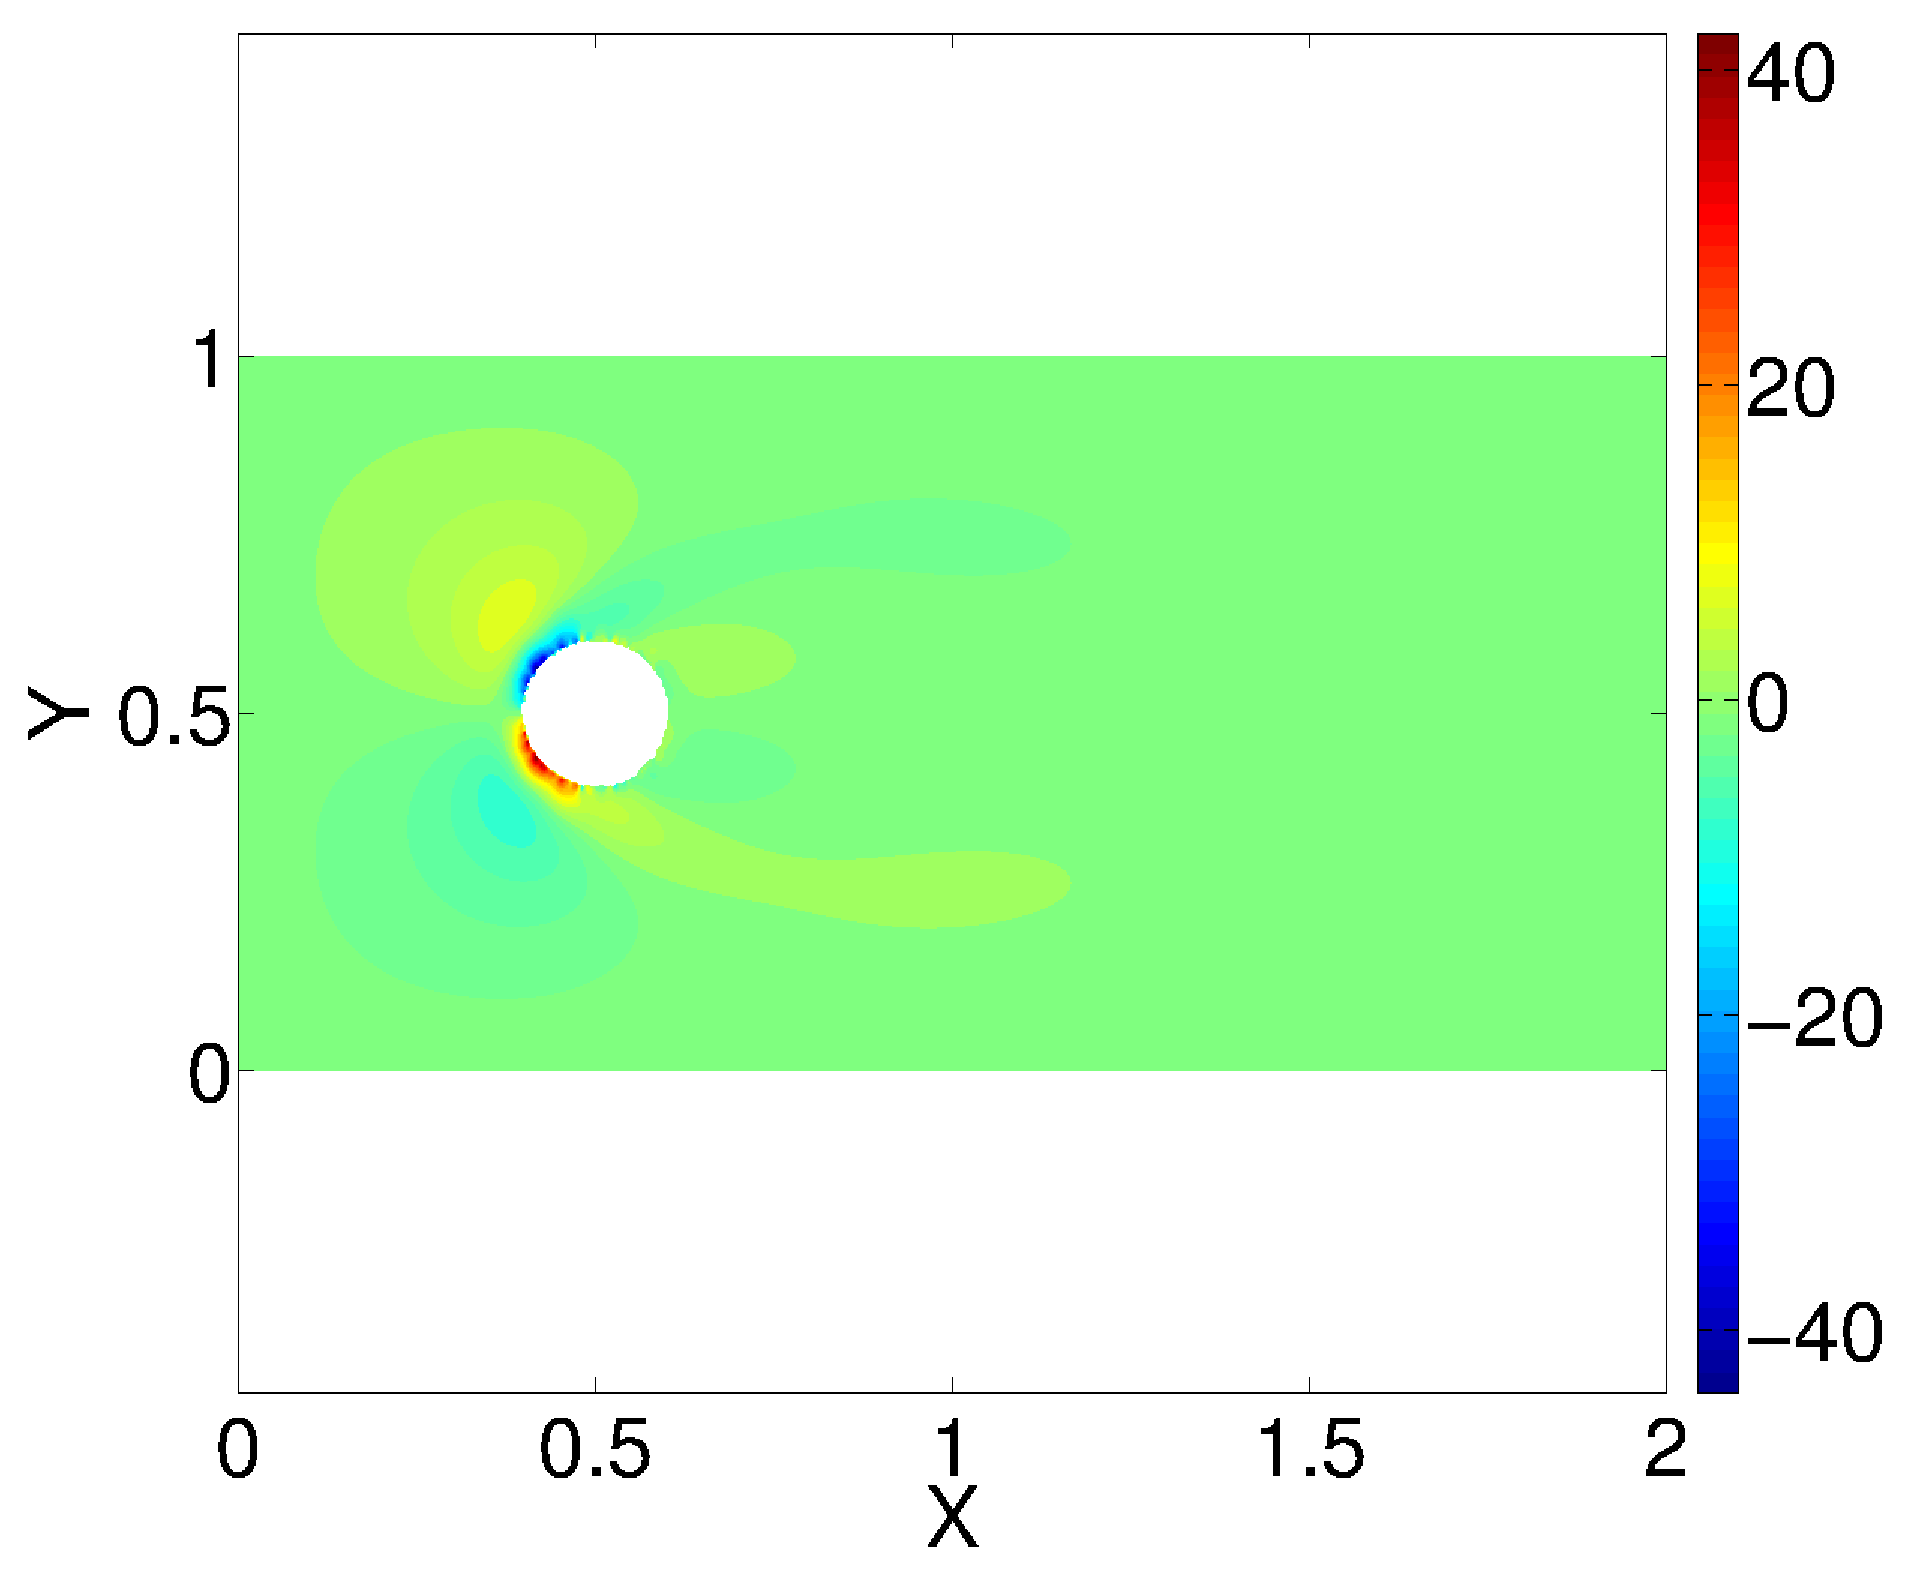
\includegraphics[height=6.0cm]{figure/cylinder/Vp_RE100.eps}
	}
	\quad
	\subfigure[Complex step result for v-velocity sensitivity]
	{
	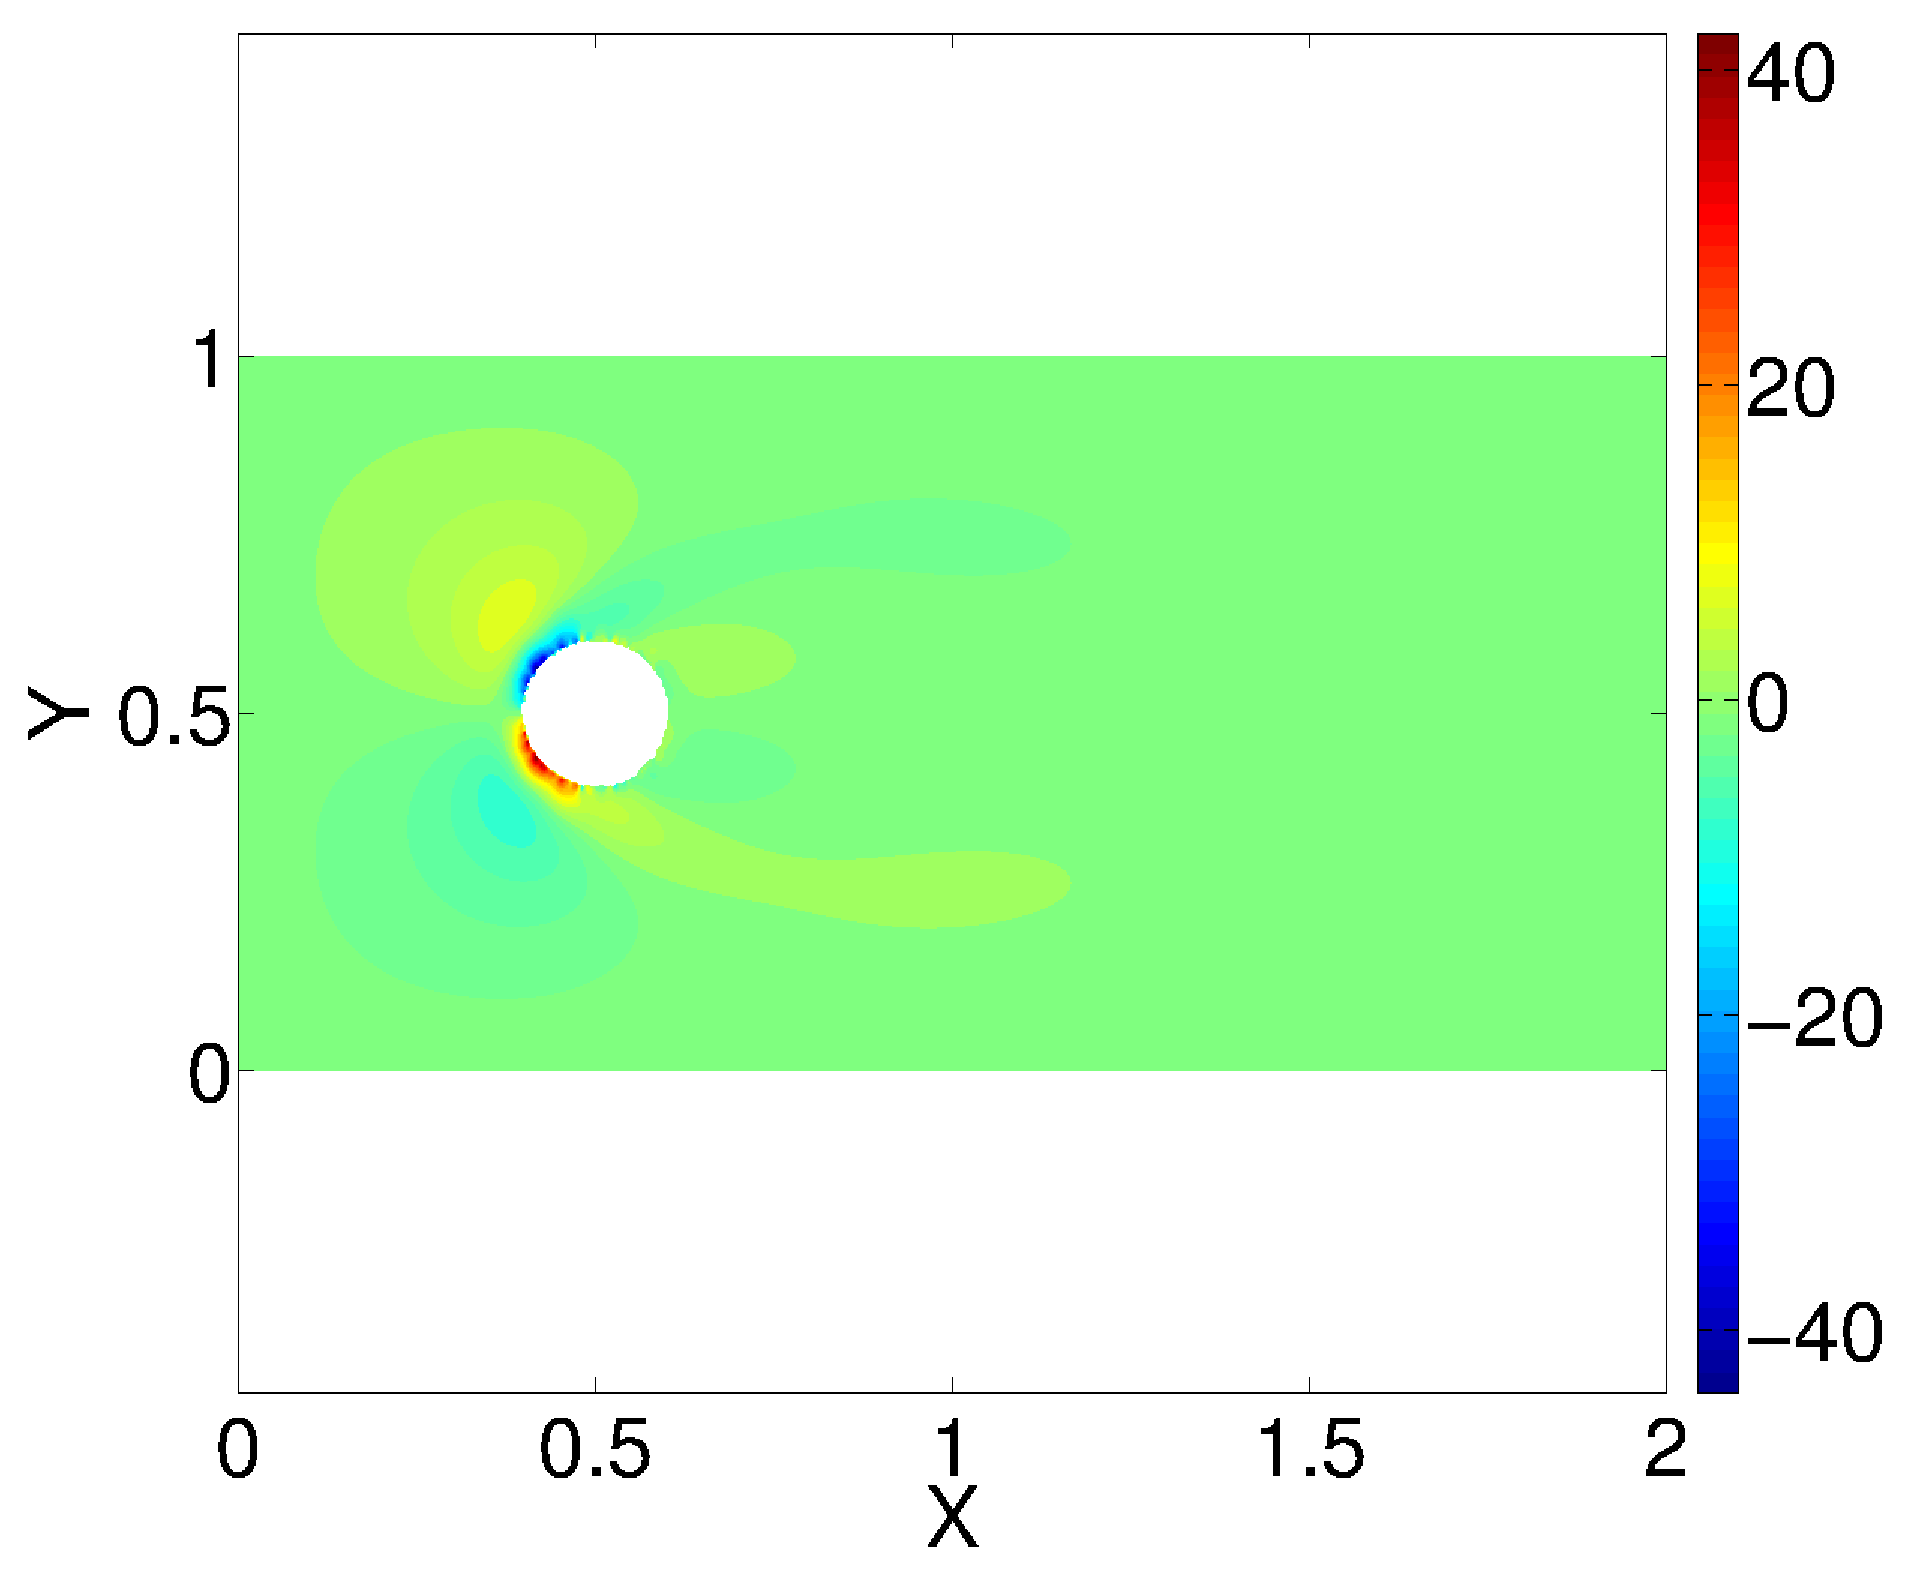
\includegraphics[height=6.0cm]{figure/cylinder/Vp_RE100.eps}
	}
	\caption{Comparison of sensitivity contours for flow over cylinder, $Re = 100$.}
	\label{fig:cylinderSensitivityContourRE100}
\end{figure}
%

%
\begin{figure}[H]
	\centering
	\subfigure[Continuum sensitivity result for pressure sensitivity]
	{
	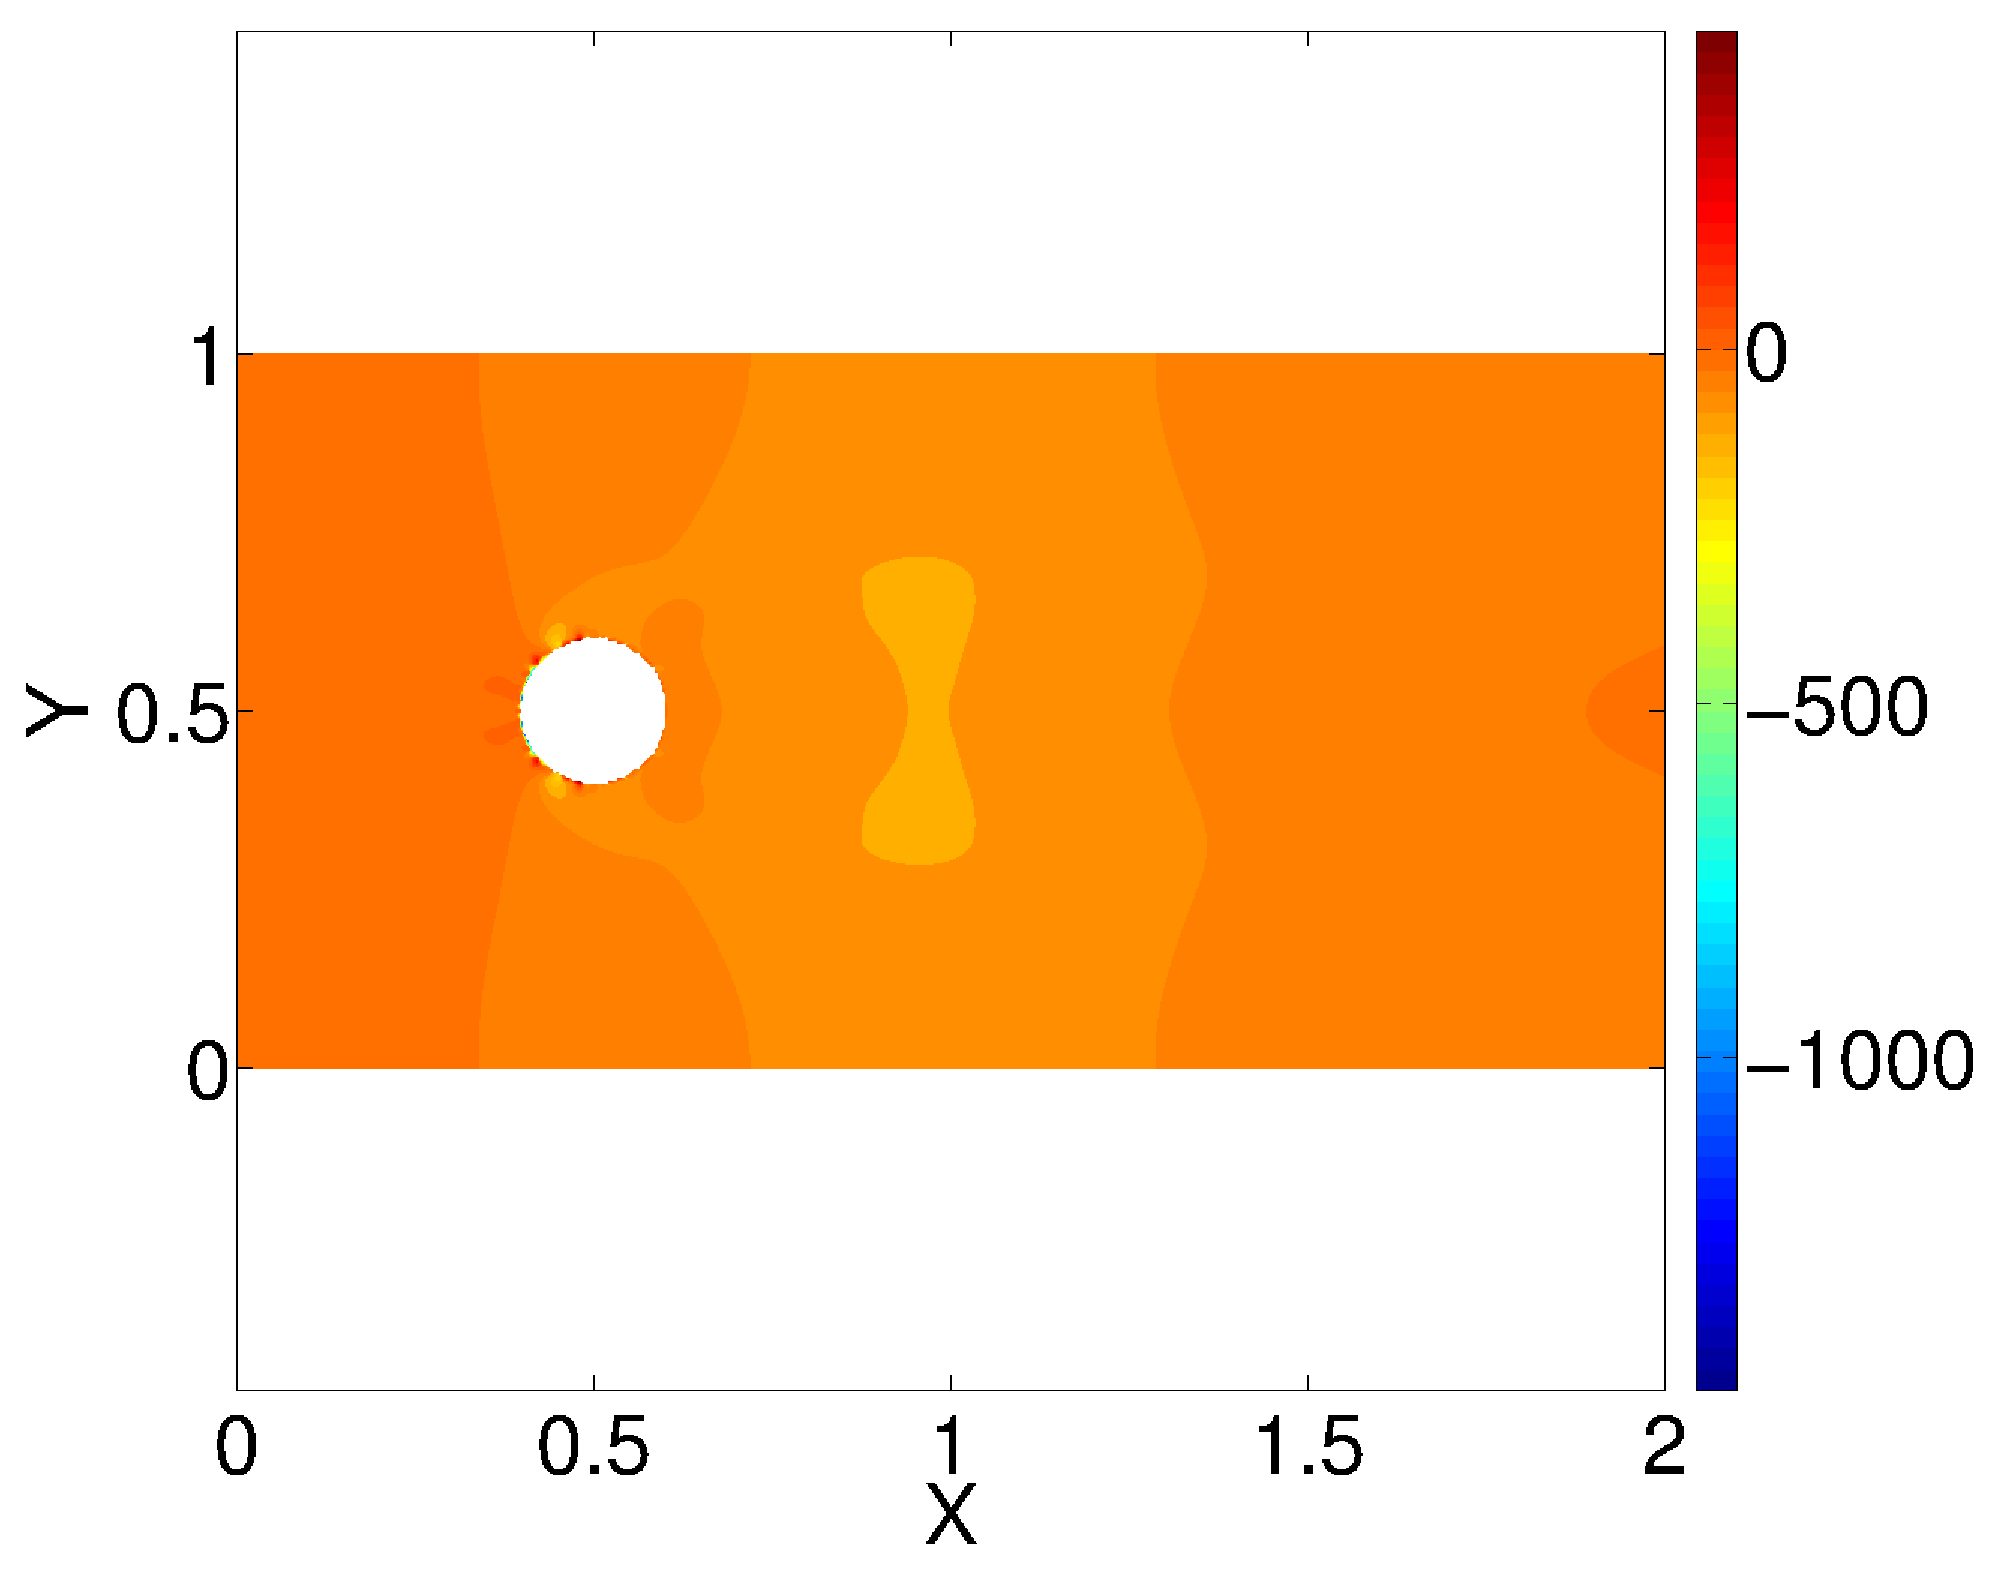
\includegraphics[height=6.0cm]{figure/cylinder/Pp_RE1000.eps}
	}
	\quad
	\subfigure[Complex step result for pressure sensitivity]
	{
	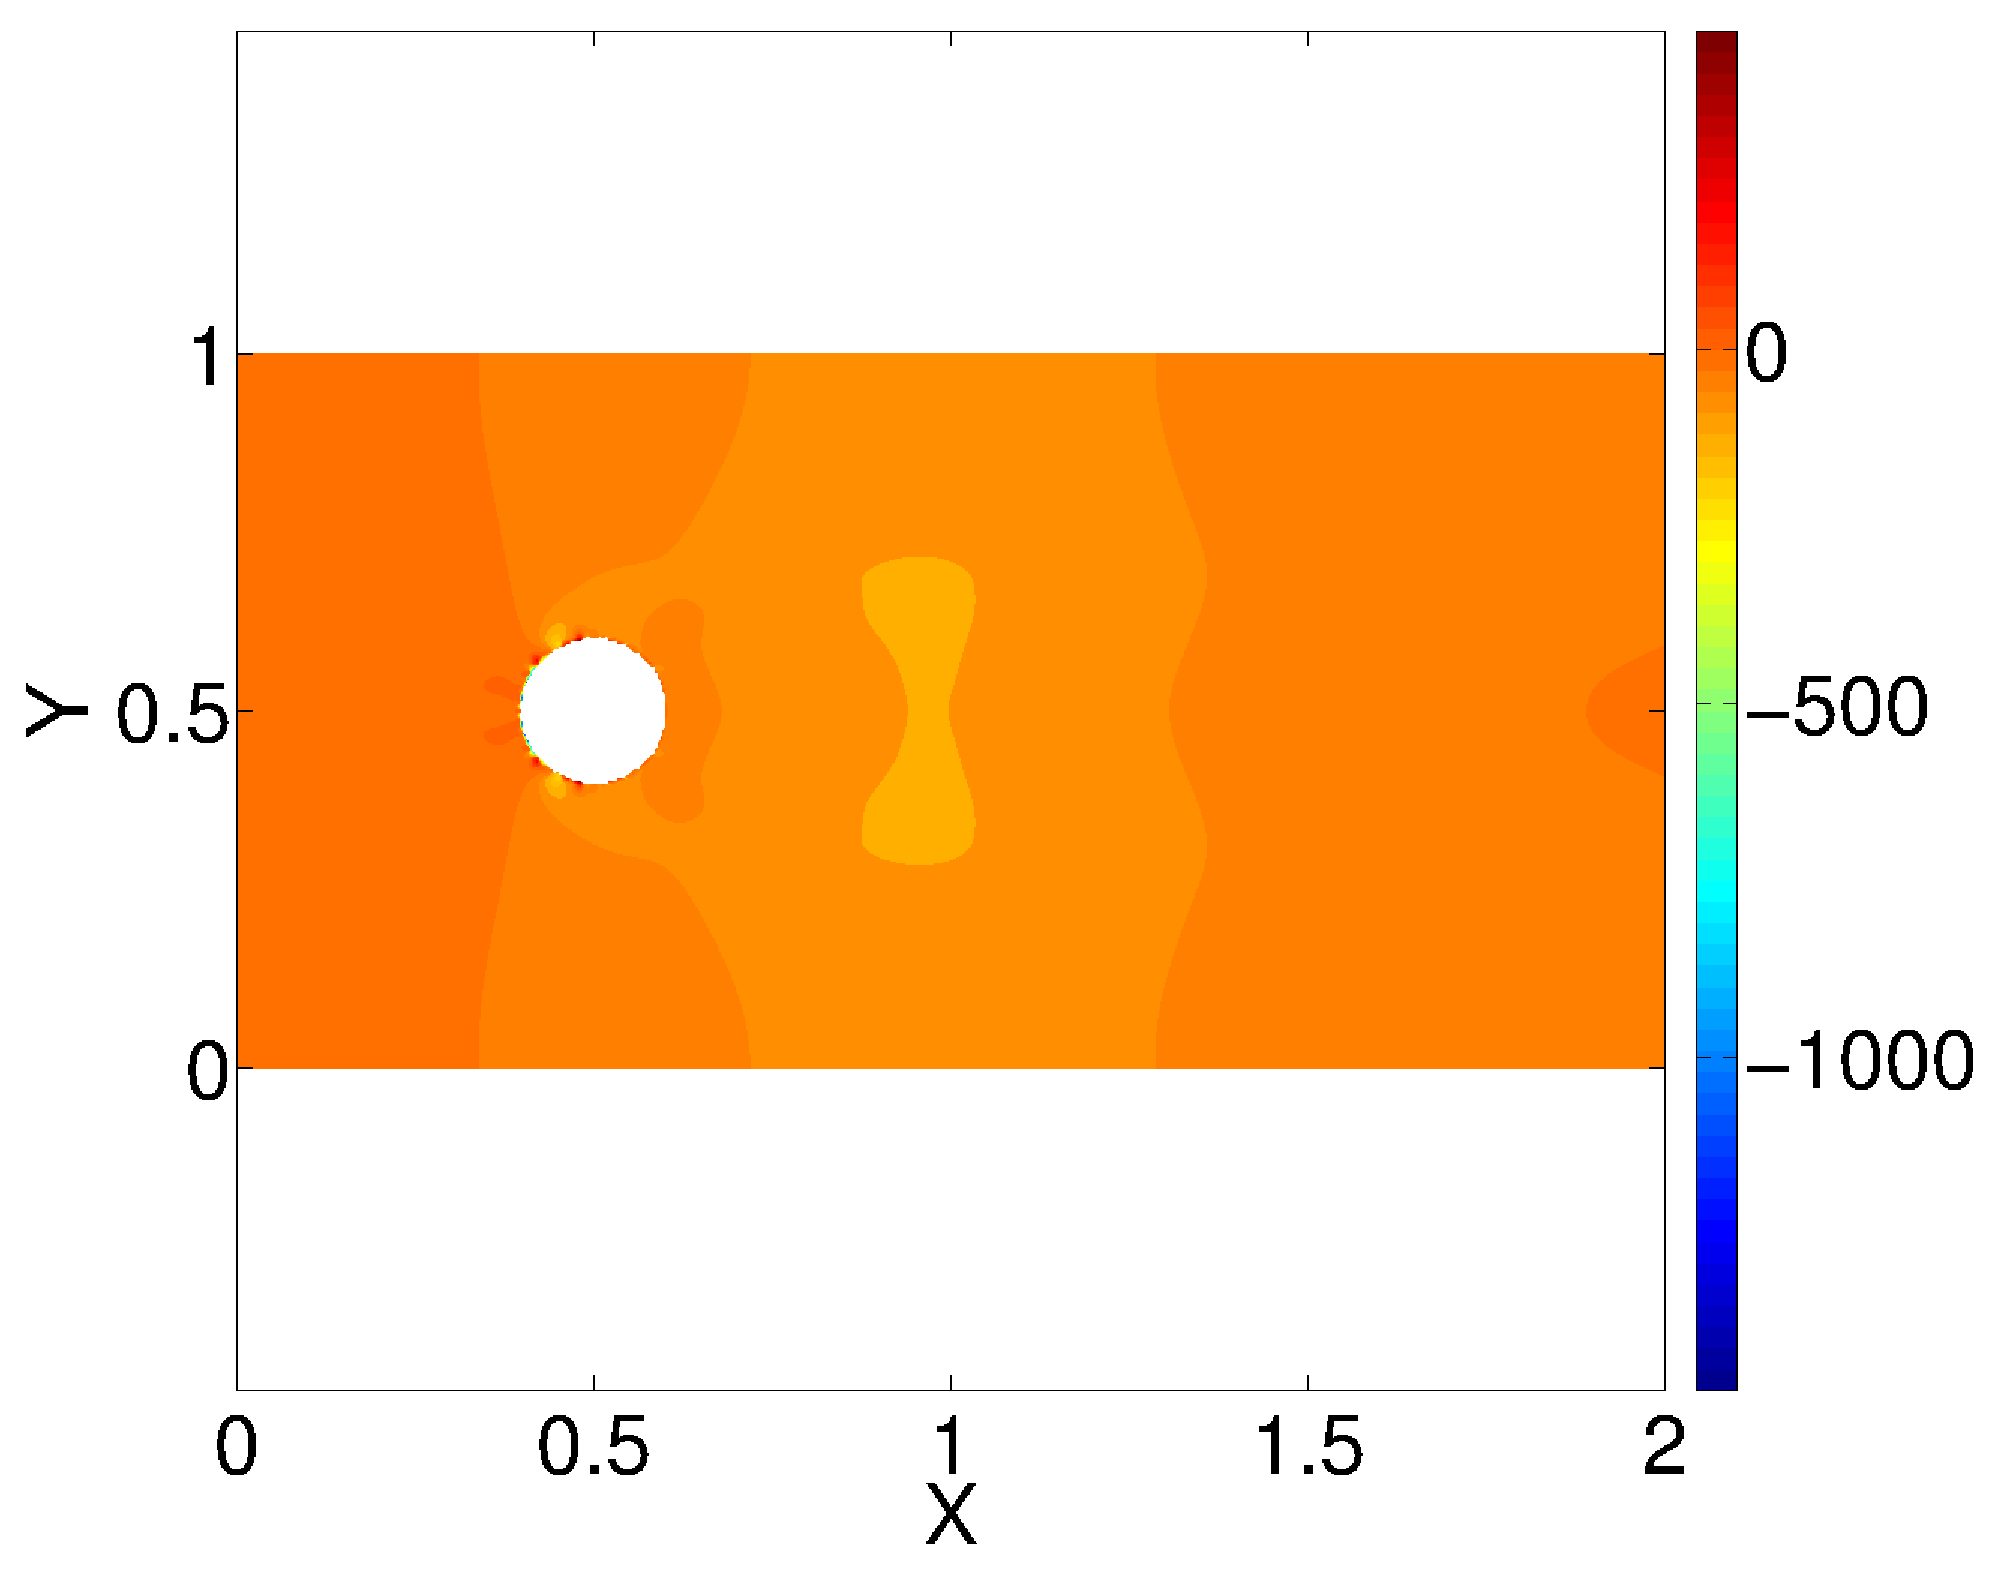
\includegraphics[height=6.0cm]{figure/cylinder/Pp_RE1000.eps}
	}
	\\
	\subfigure[Continuum sensitivity result for u-velocity sensitivity]
	{
	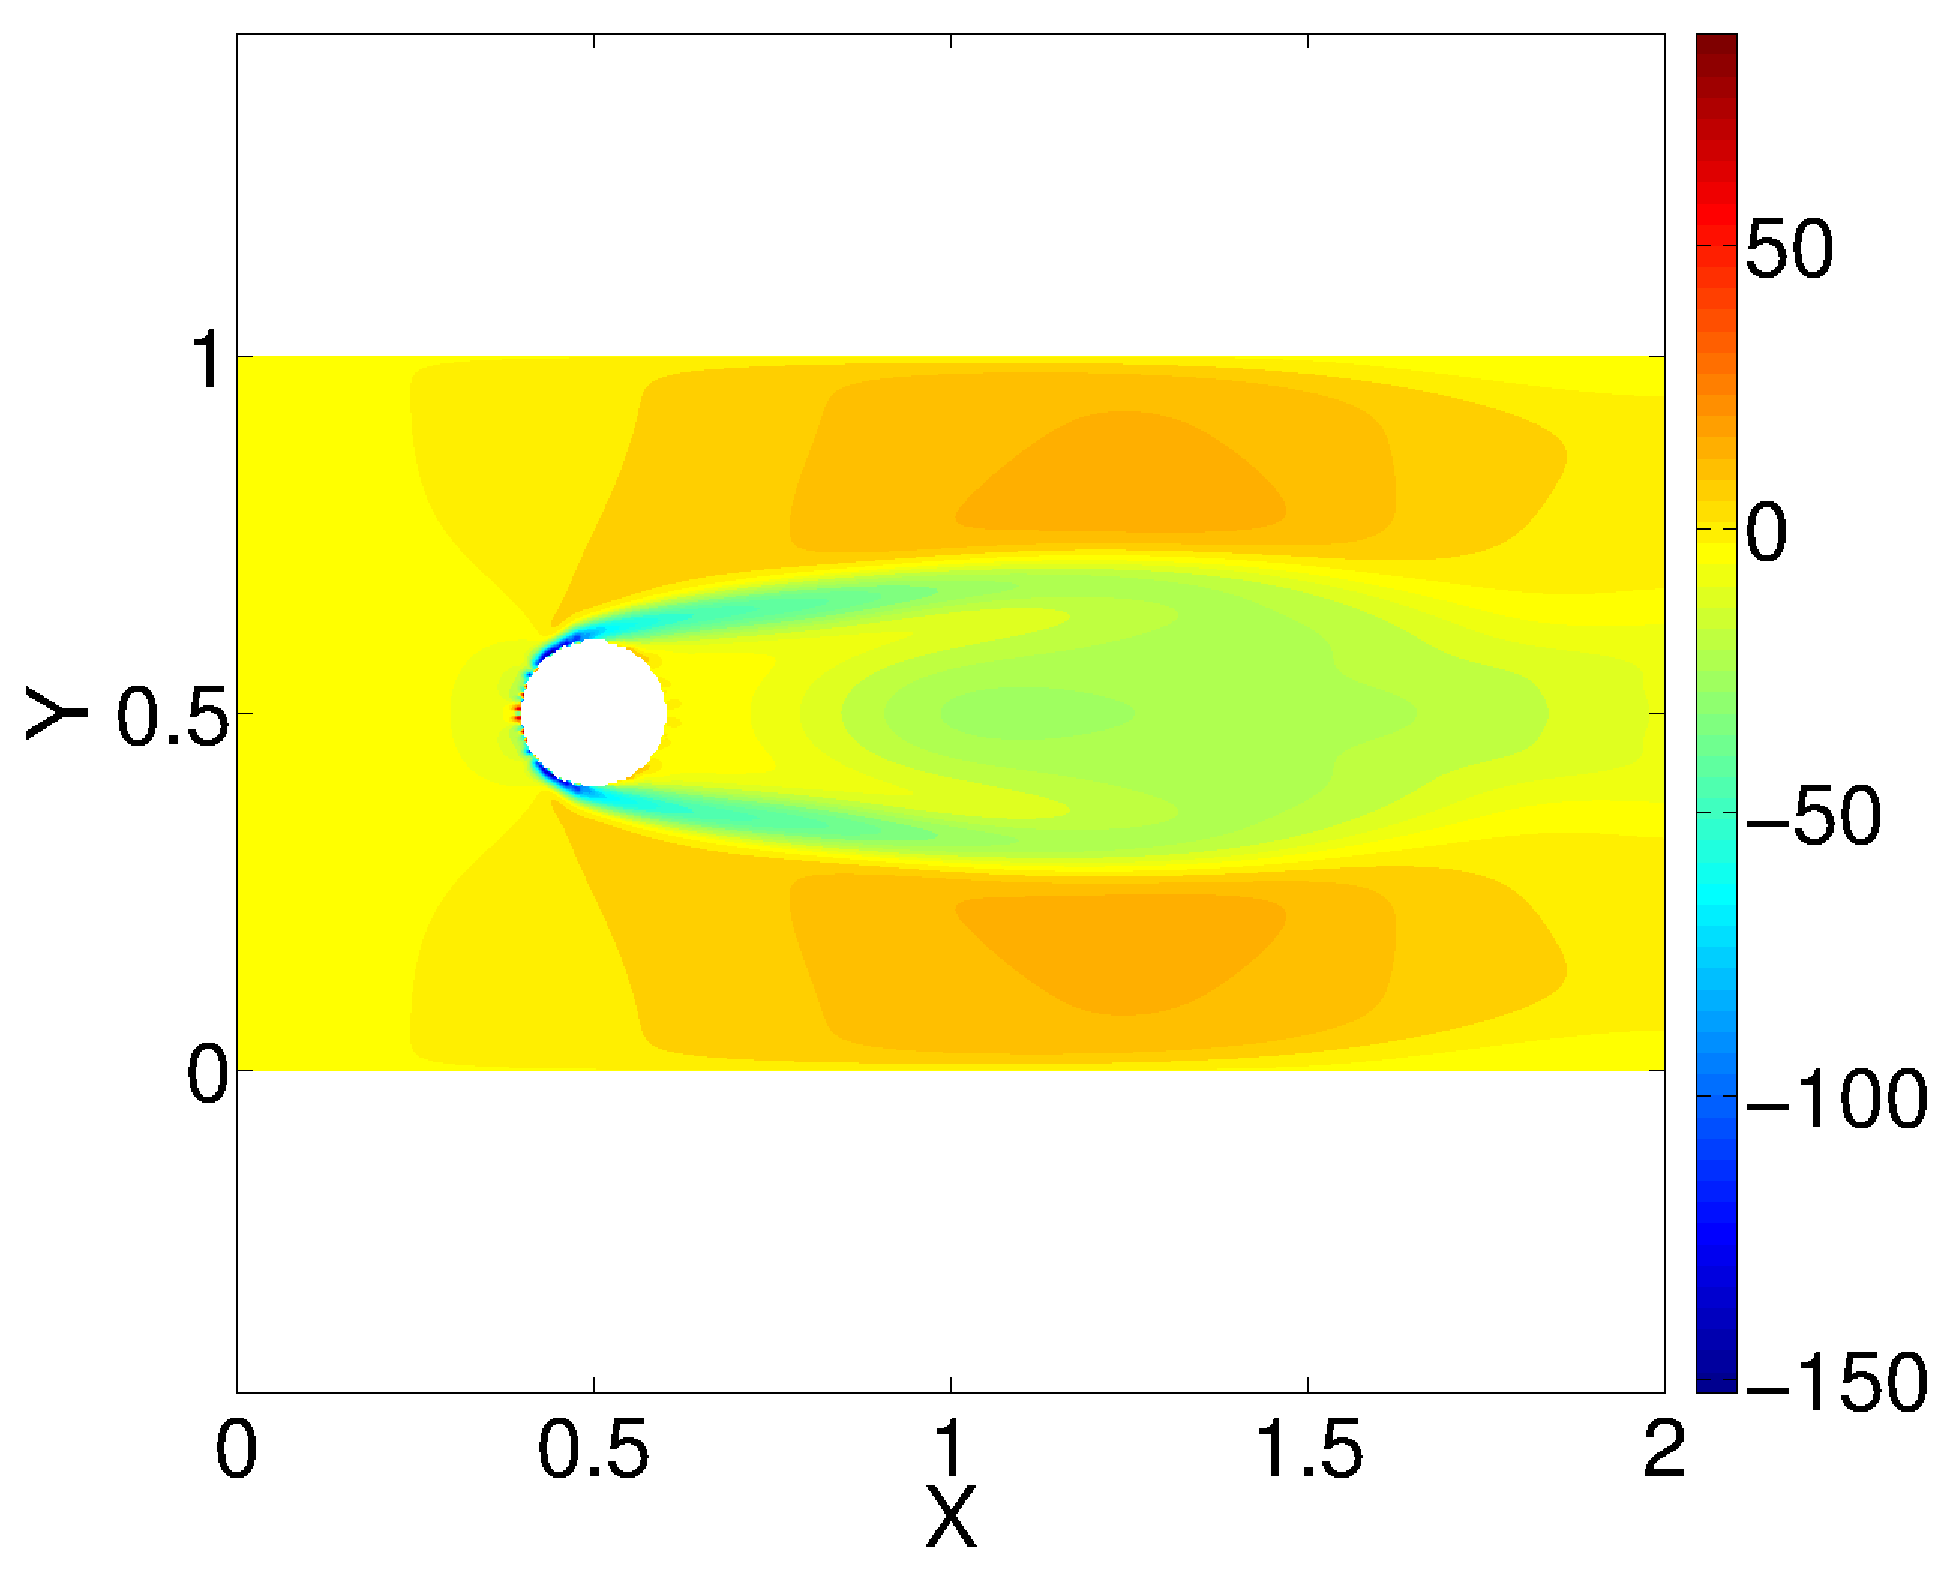
\includegraphics[height=6.0cm]{figure/cylinder/Up_RE1000.eps}
	}
	\quad
	\subfigure[Complex step result for u-velocity sensitivity]
	{
	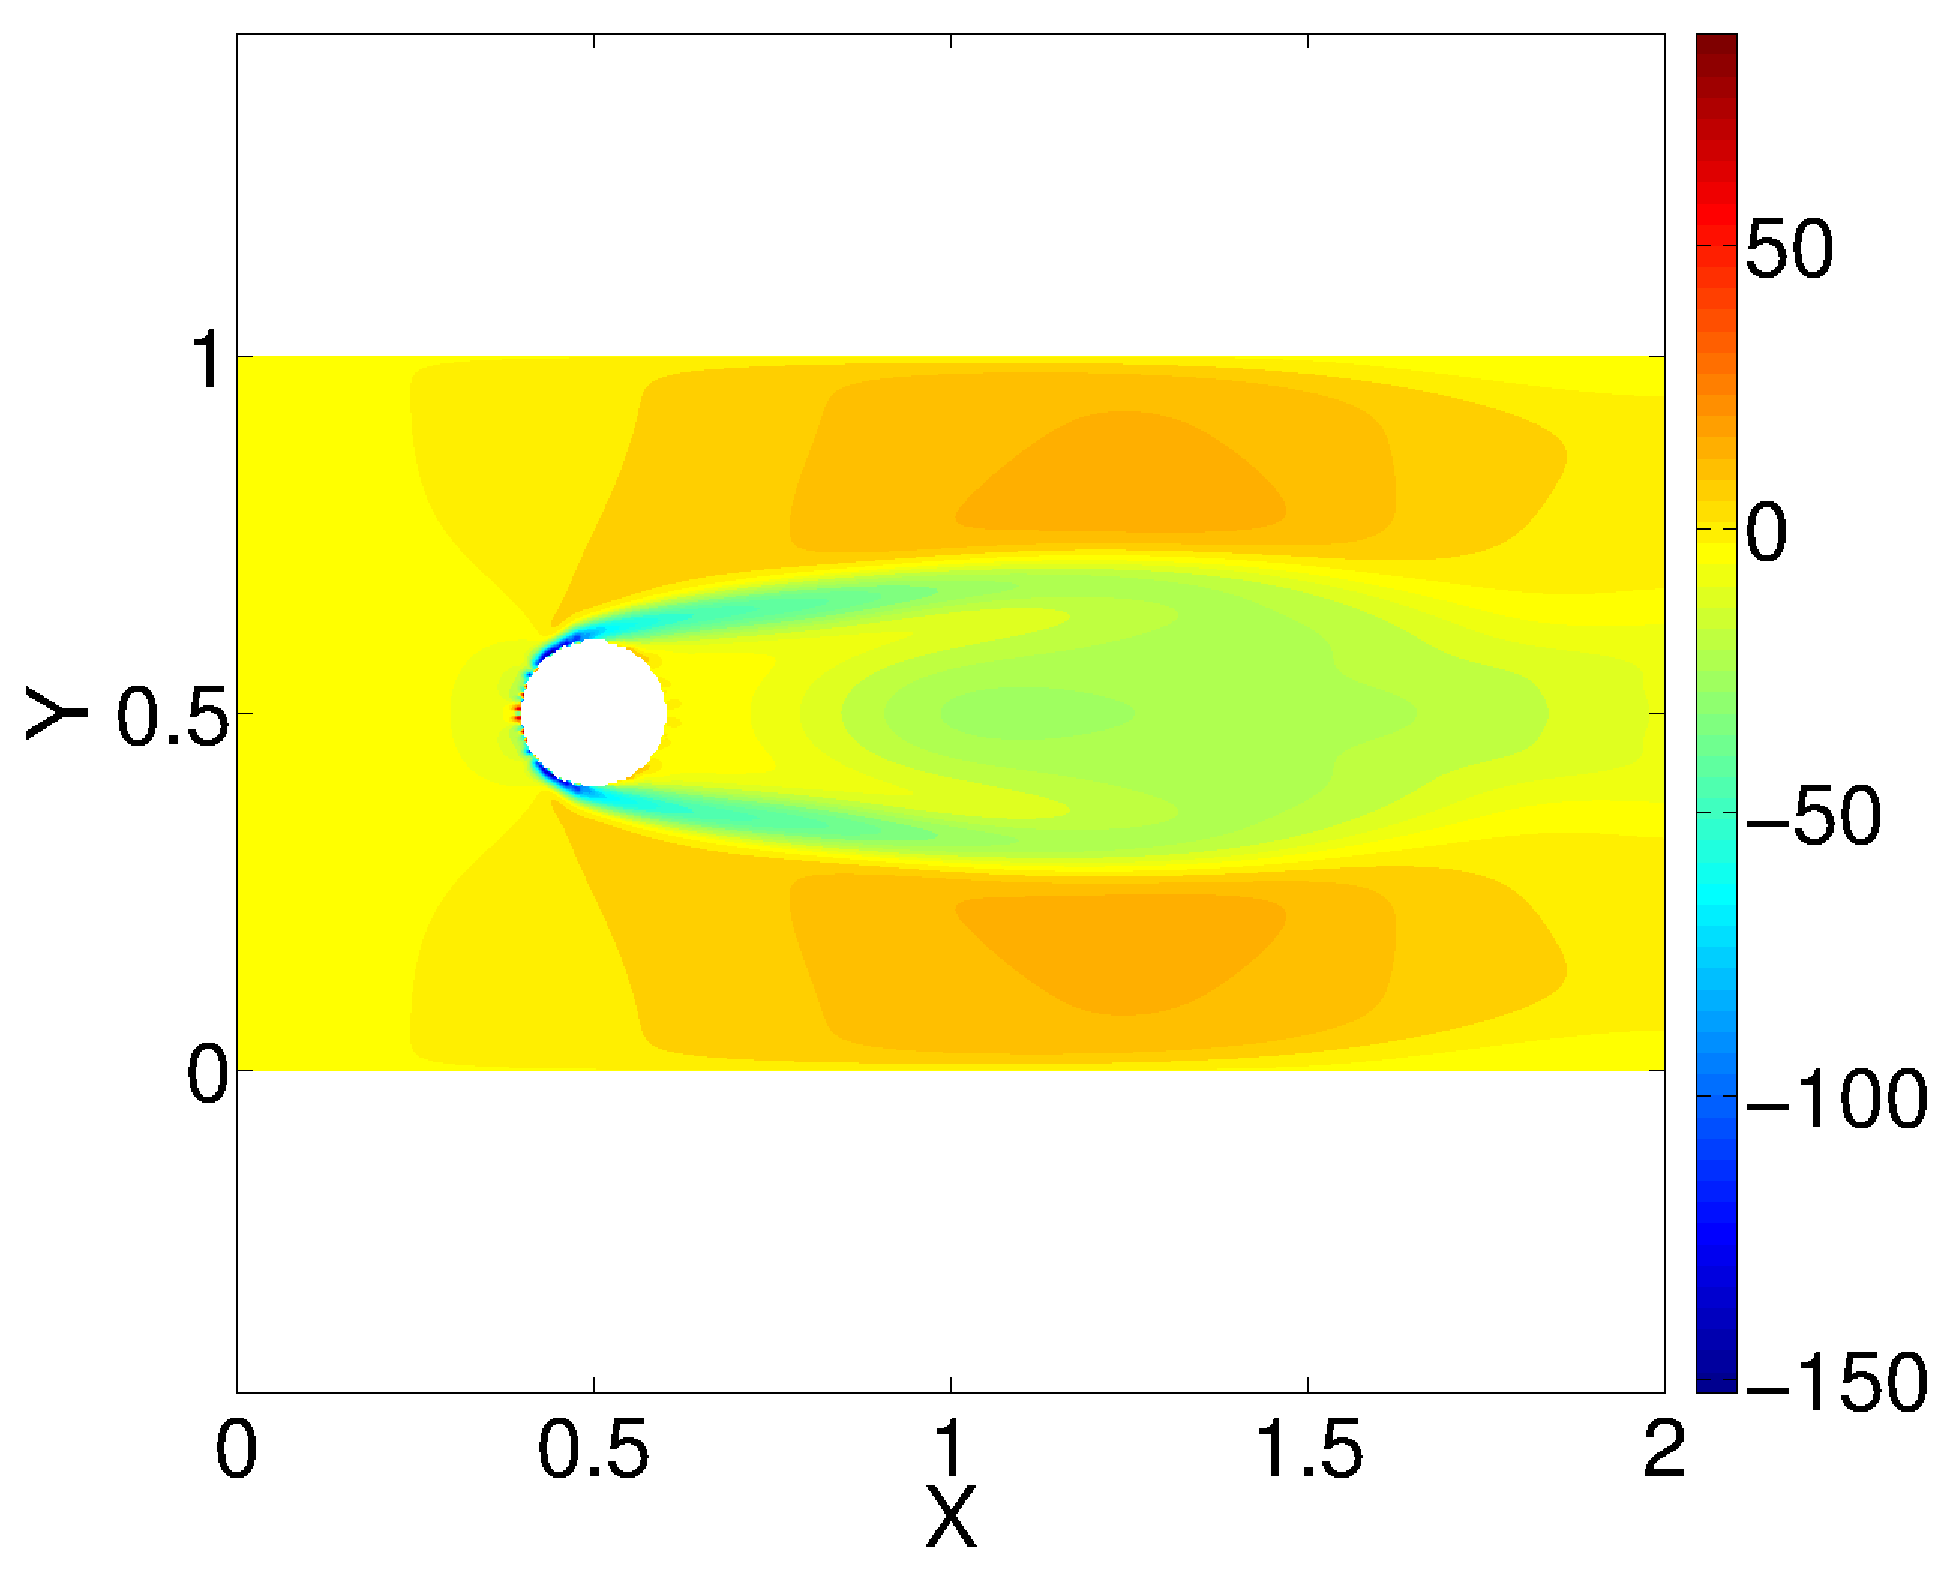
\includegraphics[height=6.0cm]{figure/cylinder/Up_RE1000.eps}
	}
	\\
	\subfigure[Continuum sensitivity result for v-velocity sensitivity]
	{
	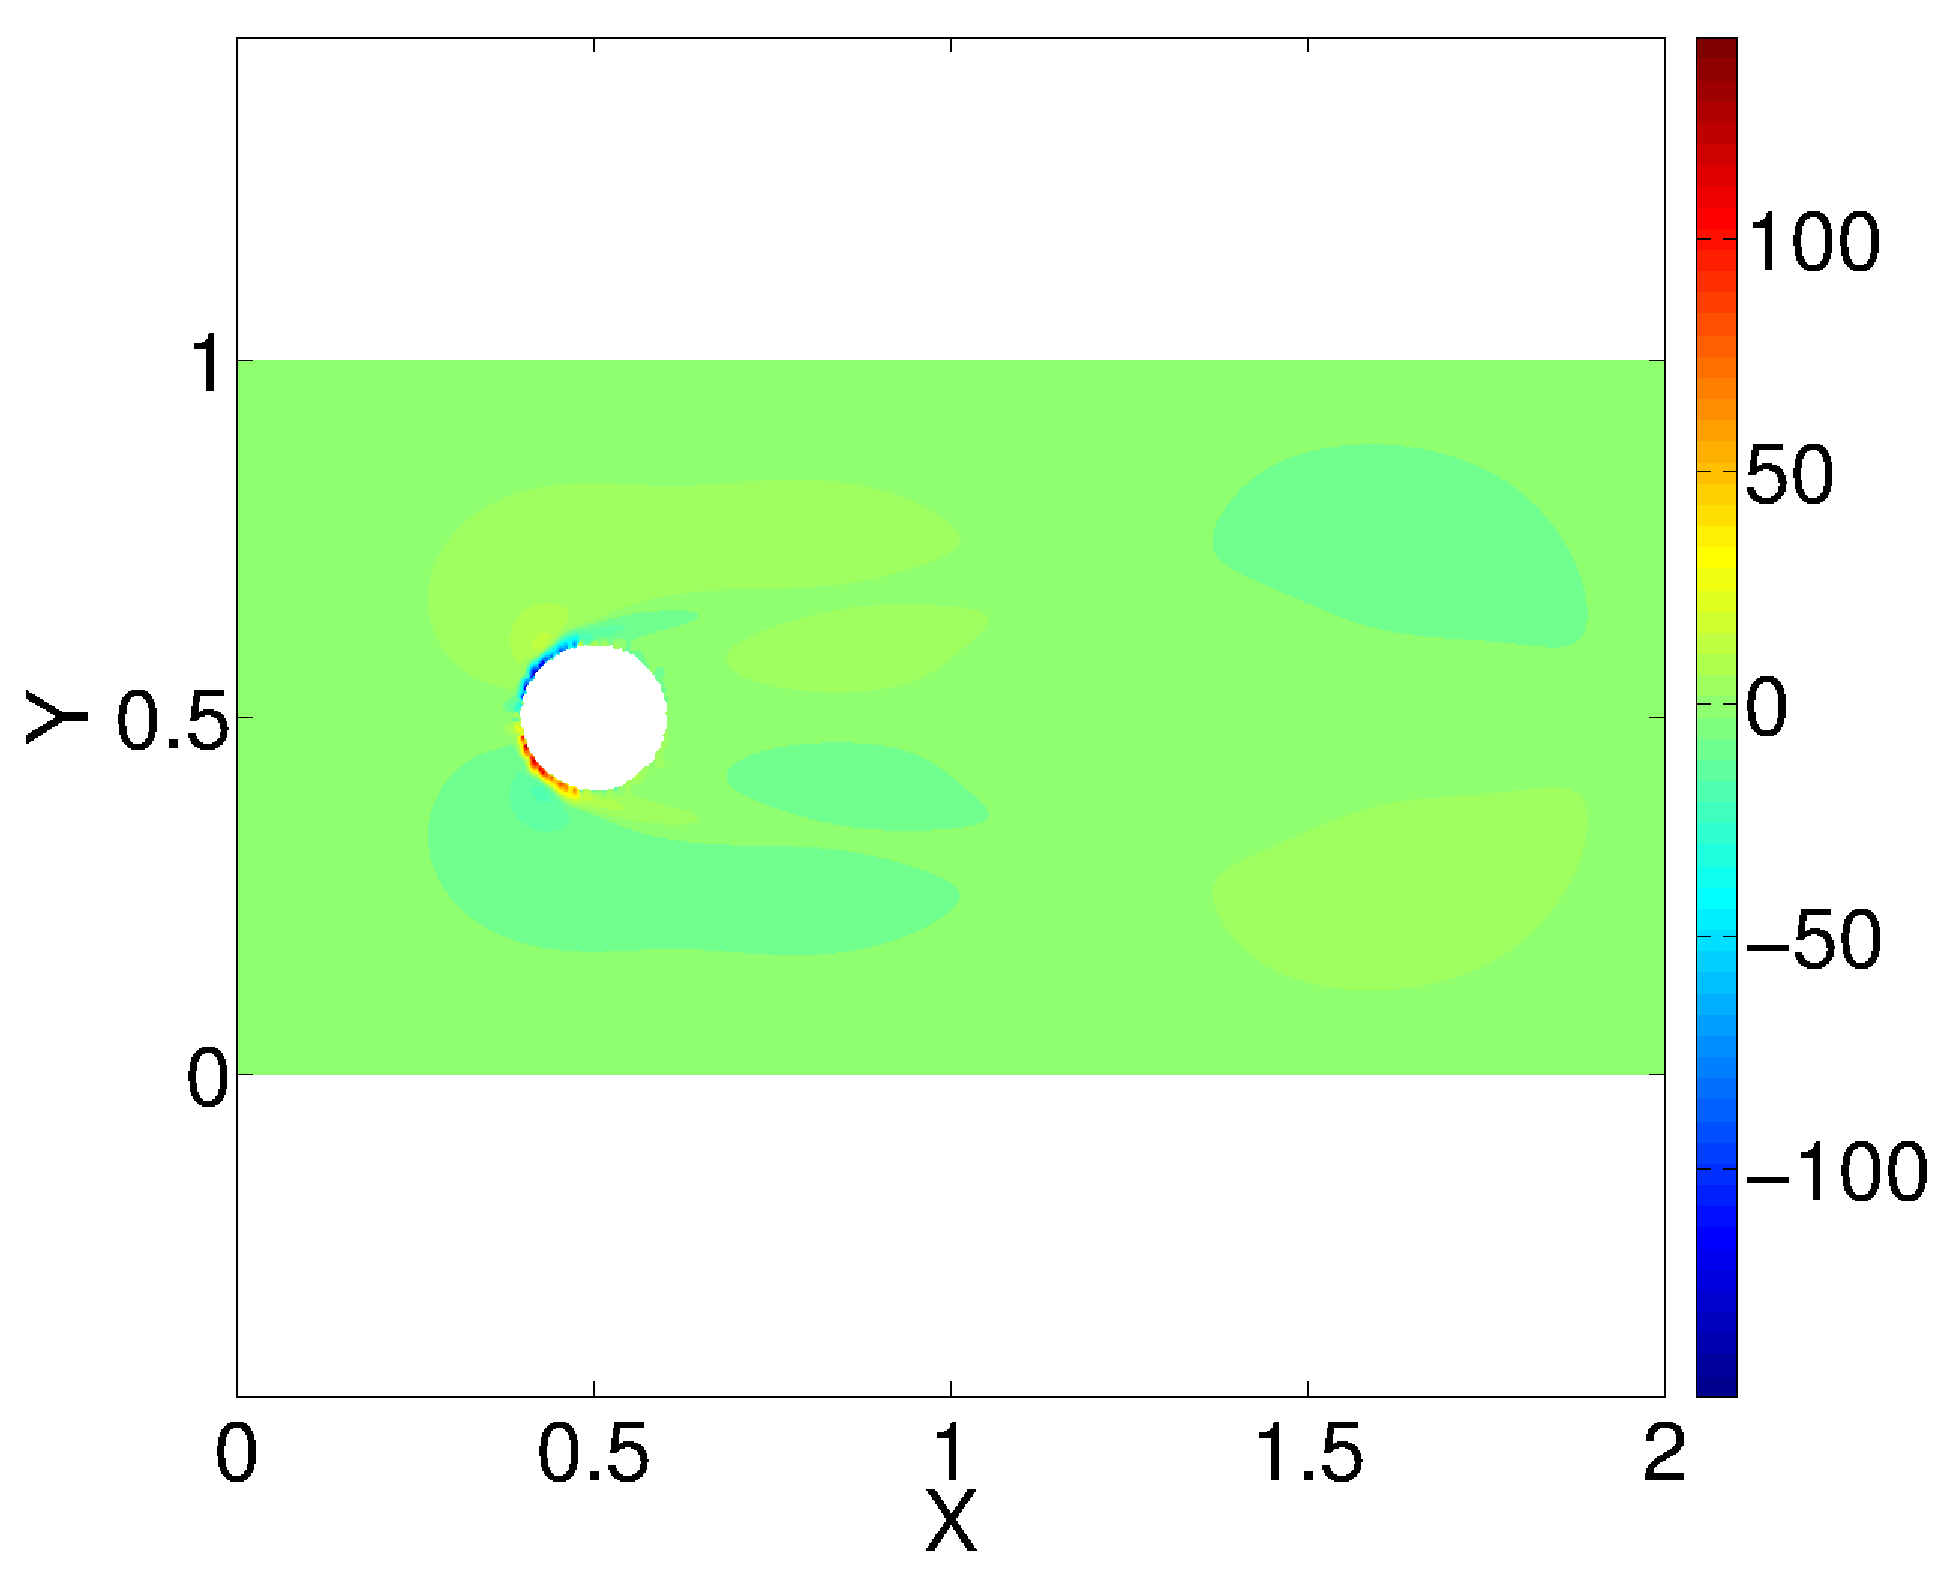
\includegraphics[height=6.0cm]{figure/cylinder/Vp_RE1000.eps}
	}
	\quad
	\subfigure[Complex step result for v-velocity sensitivity]
	{
	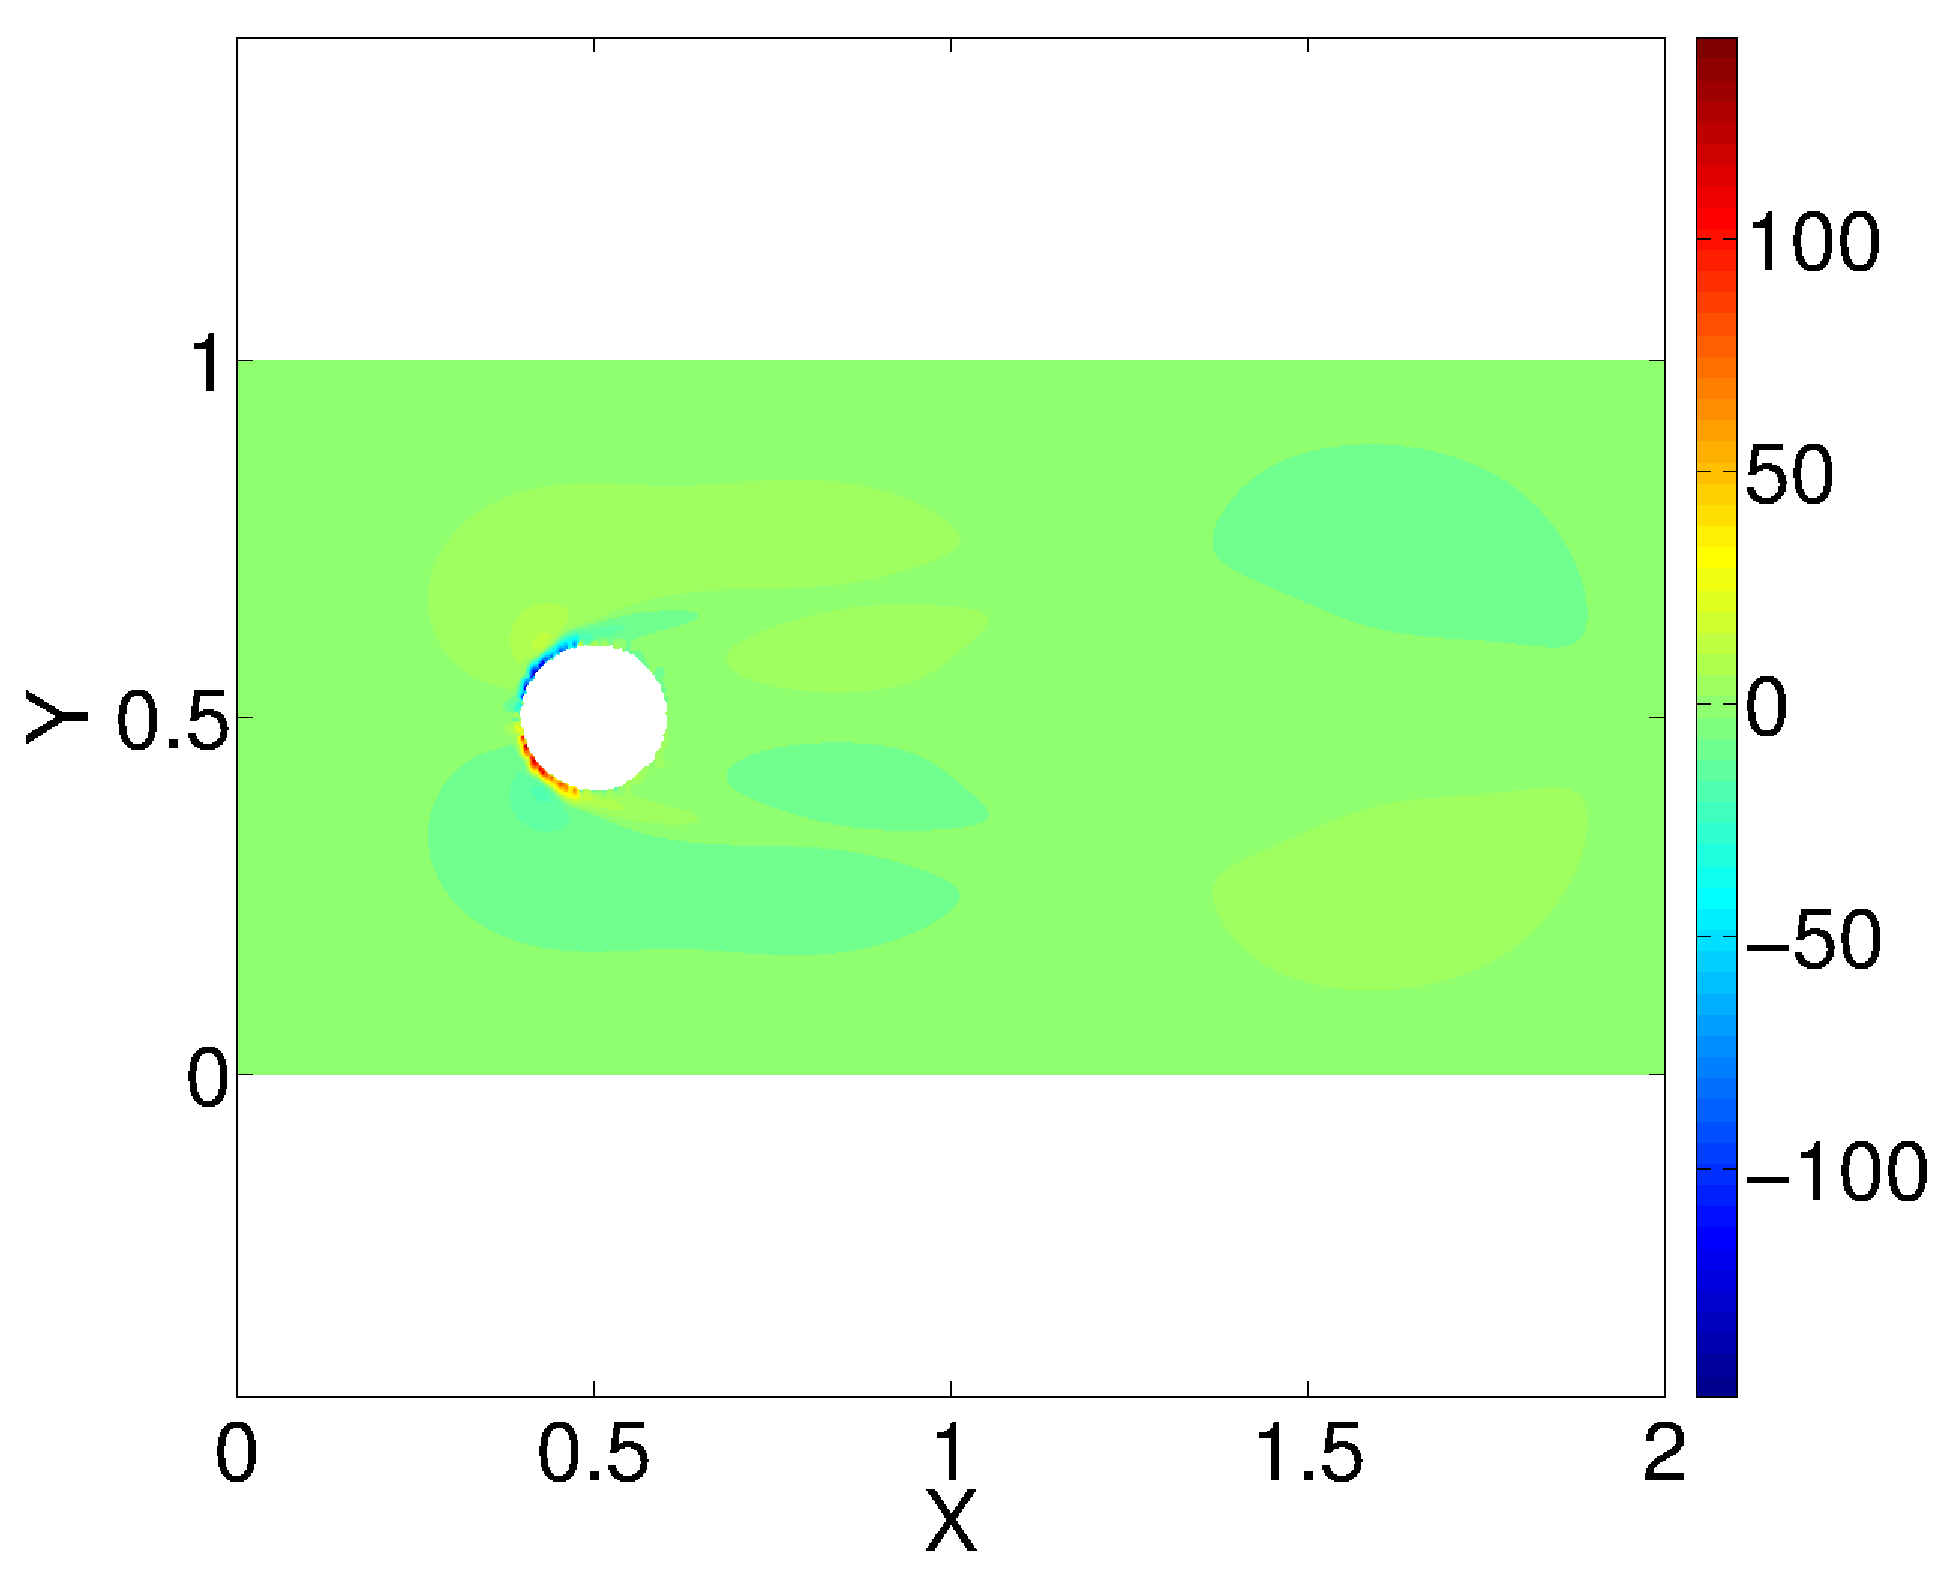
\includegraphics[height=6.0cm]{figure/cylinder/Vp_RE1000.eps}
	}
	\caption{Comparison of sensitivity contours for flow over cylinder, $Re = 1000$.}
	\label{fig:cylinderSensitivityContourRE1000}
\end{figure}
%

For a better comparison between the sensitivity results of continuum sensitivity analysis and complex step method, we looked at different locations in the computational domain. These locations are indicated in Figure \ref{fig:cylinderSampleLocations}.

%
\begin{figure}[H]
	\centering
	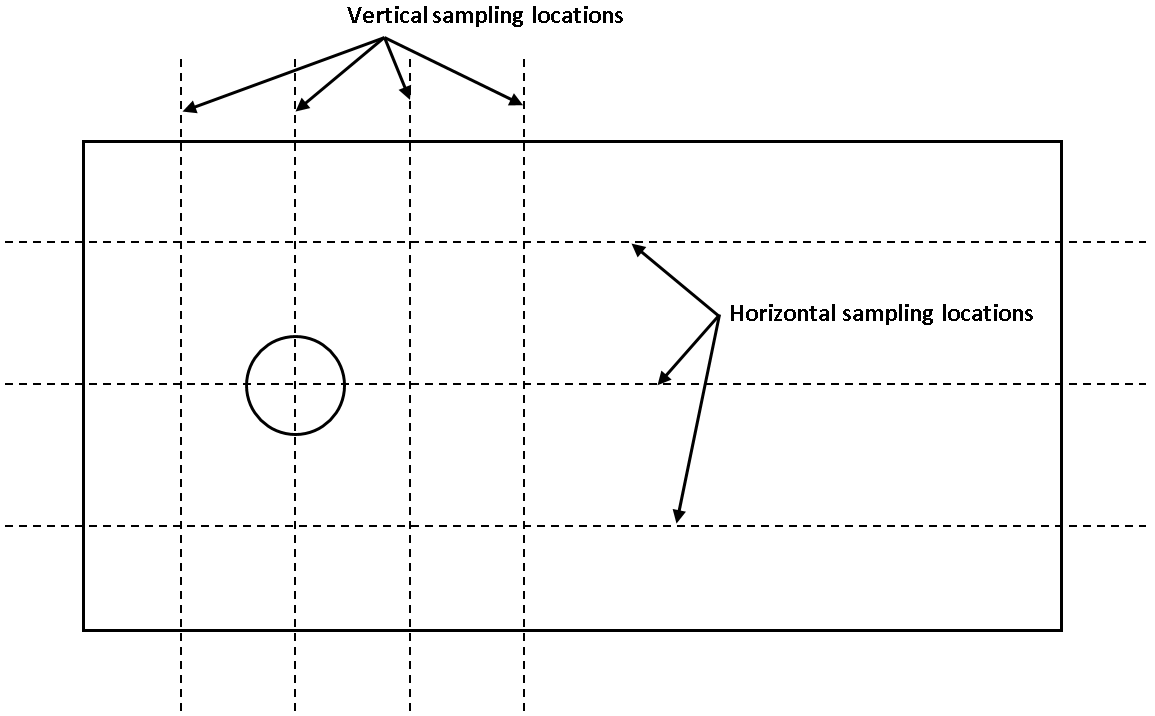
\includegraphics[height=5.0cm]{figure/cylinder/sampling_location.png}
	\caption{Sampling location for the sensitivities}
	\label{fig:cylinderSampleLocations}
\end{figure}
%

We compared the sensitivity of u-velocity and pressure on sample location for different values of Reynolds number. As shown in Figures \ref{fig:cylinderPressureSensitivity} and \ref{fig:cylinderVelocitySensitivity}, the continuum sensitivity and complex step results agree well with each other.

%
\begin{figure}[H]
	\centering
	\subfigure[y = 0.25, Re = 100]
	{
	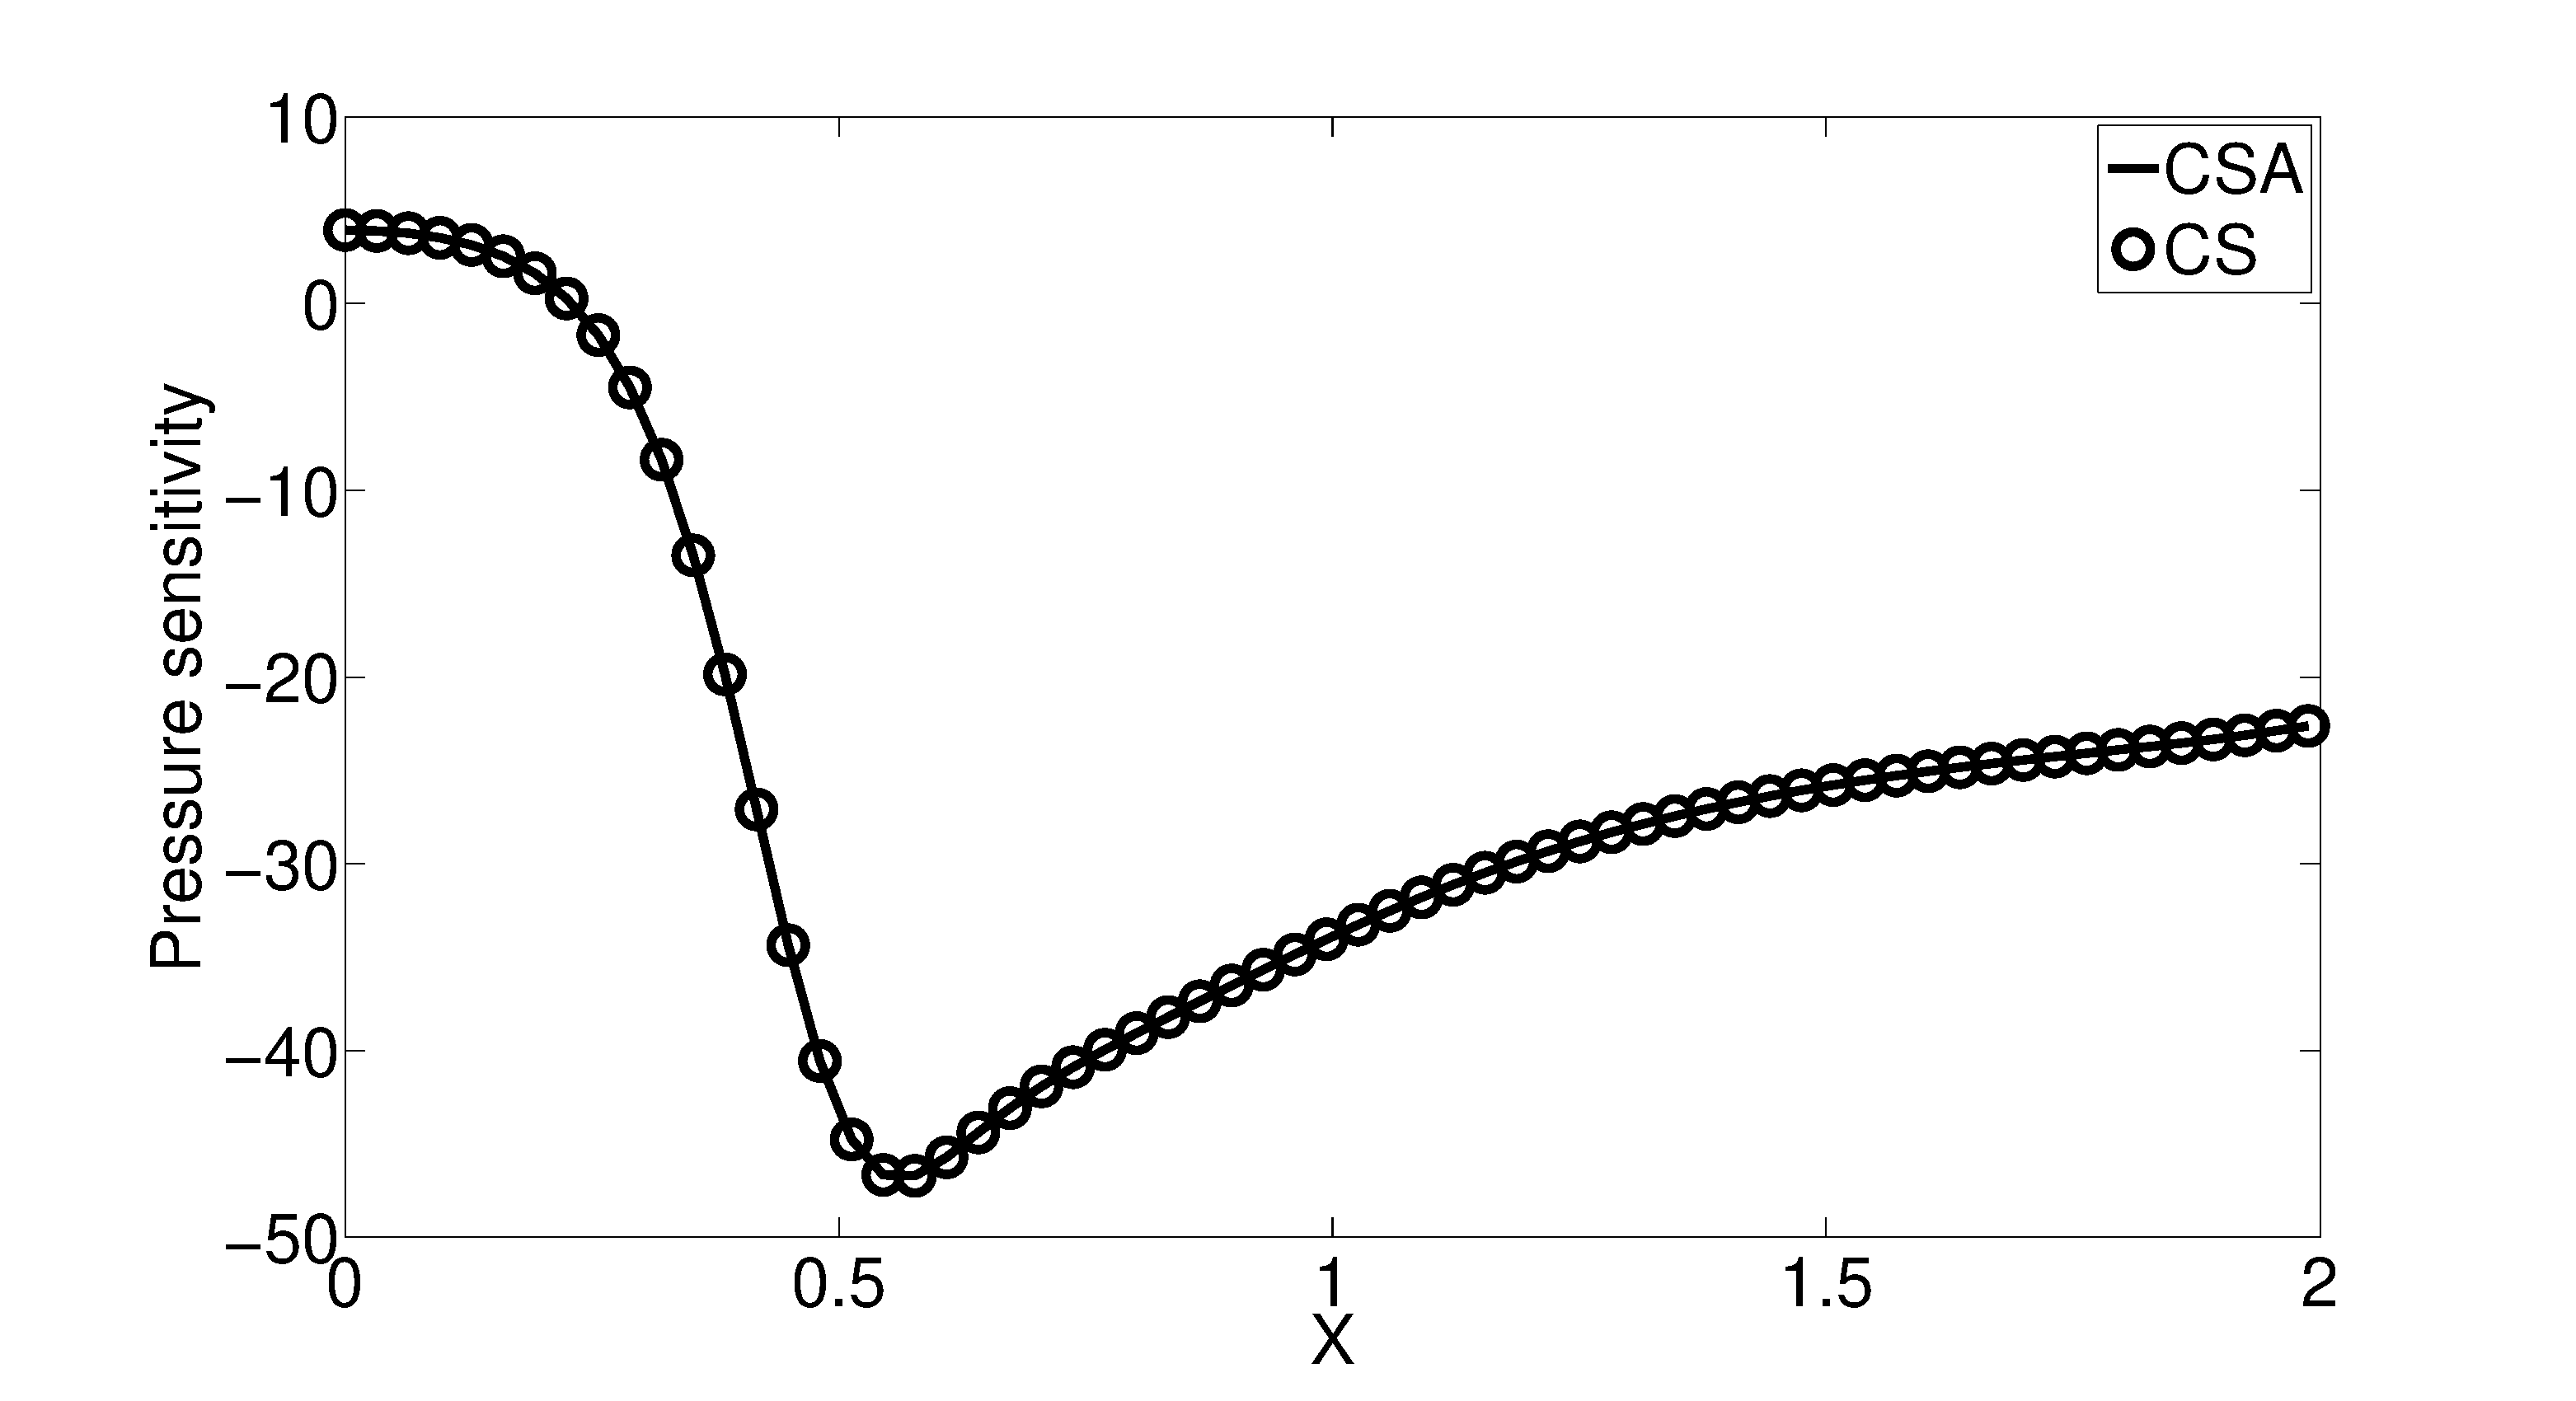
\includegraphics[height=4.0cm]{figure/cylinder/Pp025_RE100.eps}
	}
	\quad
	\subfigure[y = 0.25, Re = 1000]
	{
	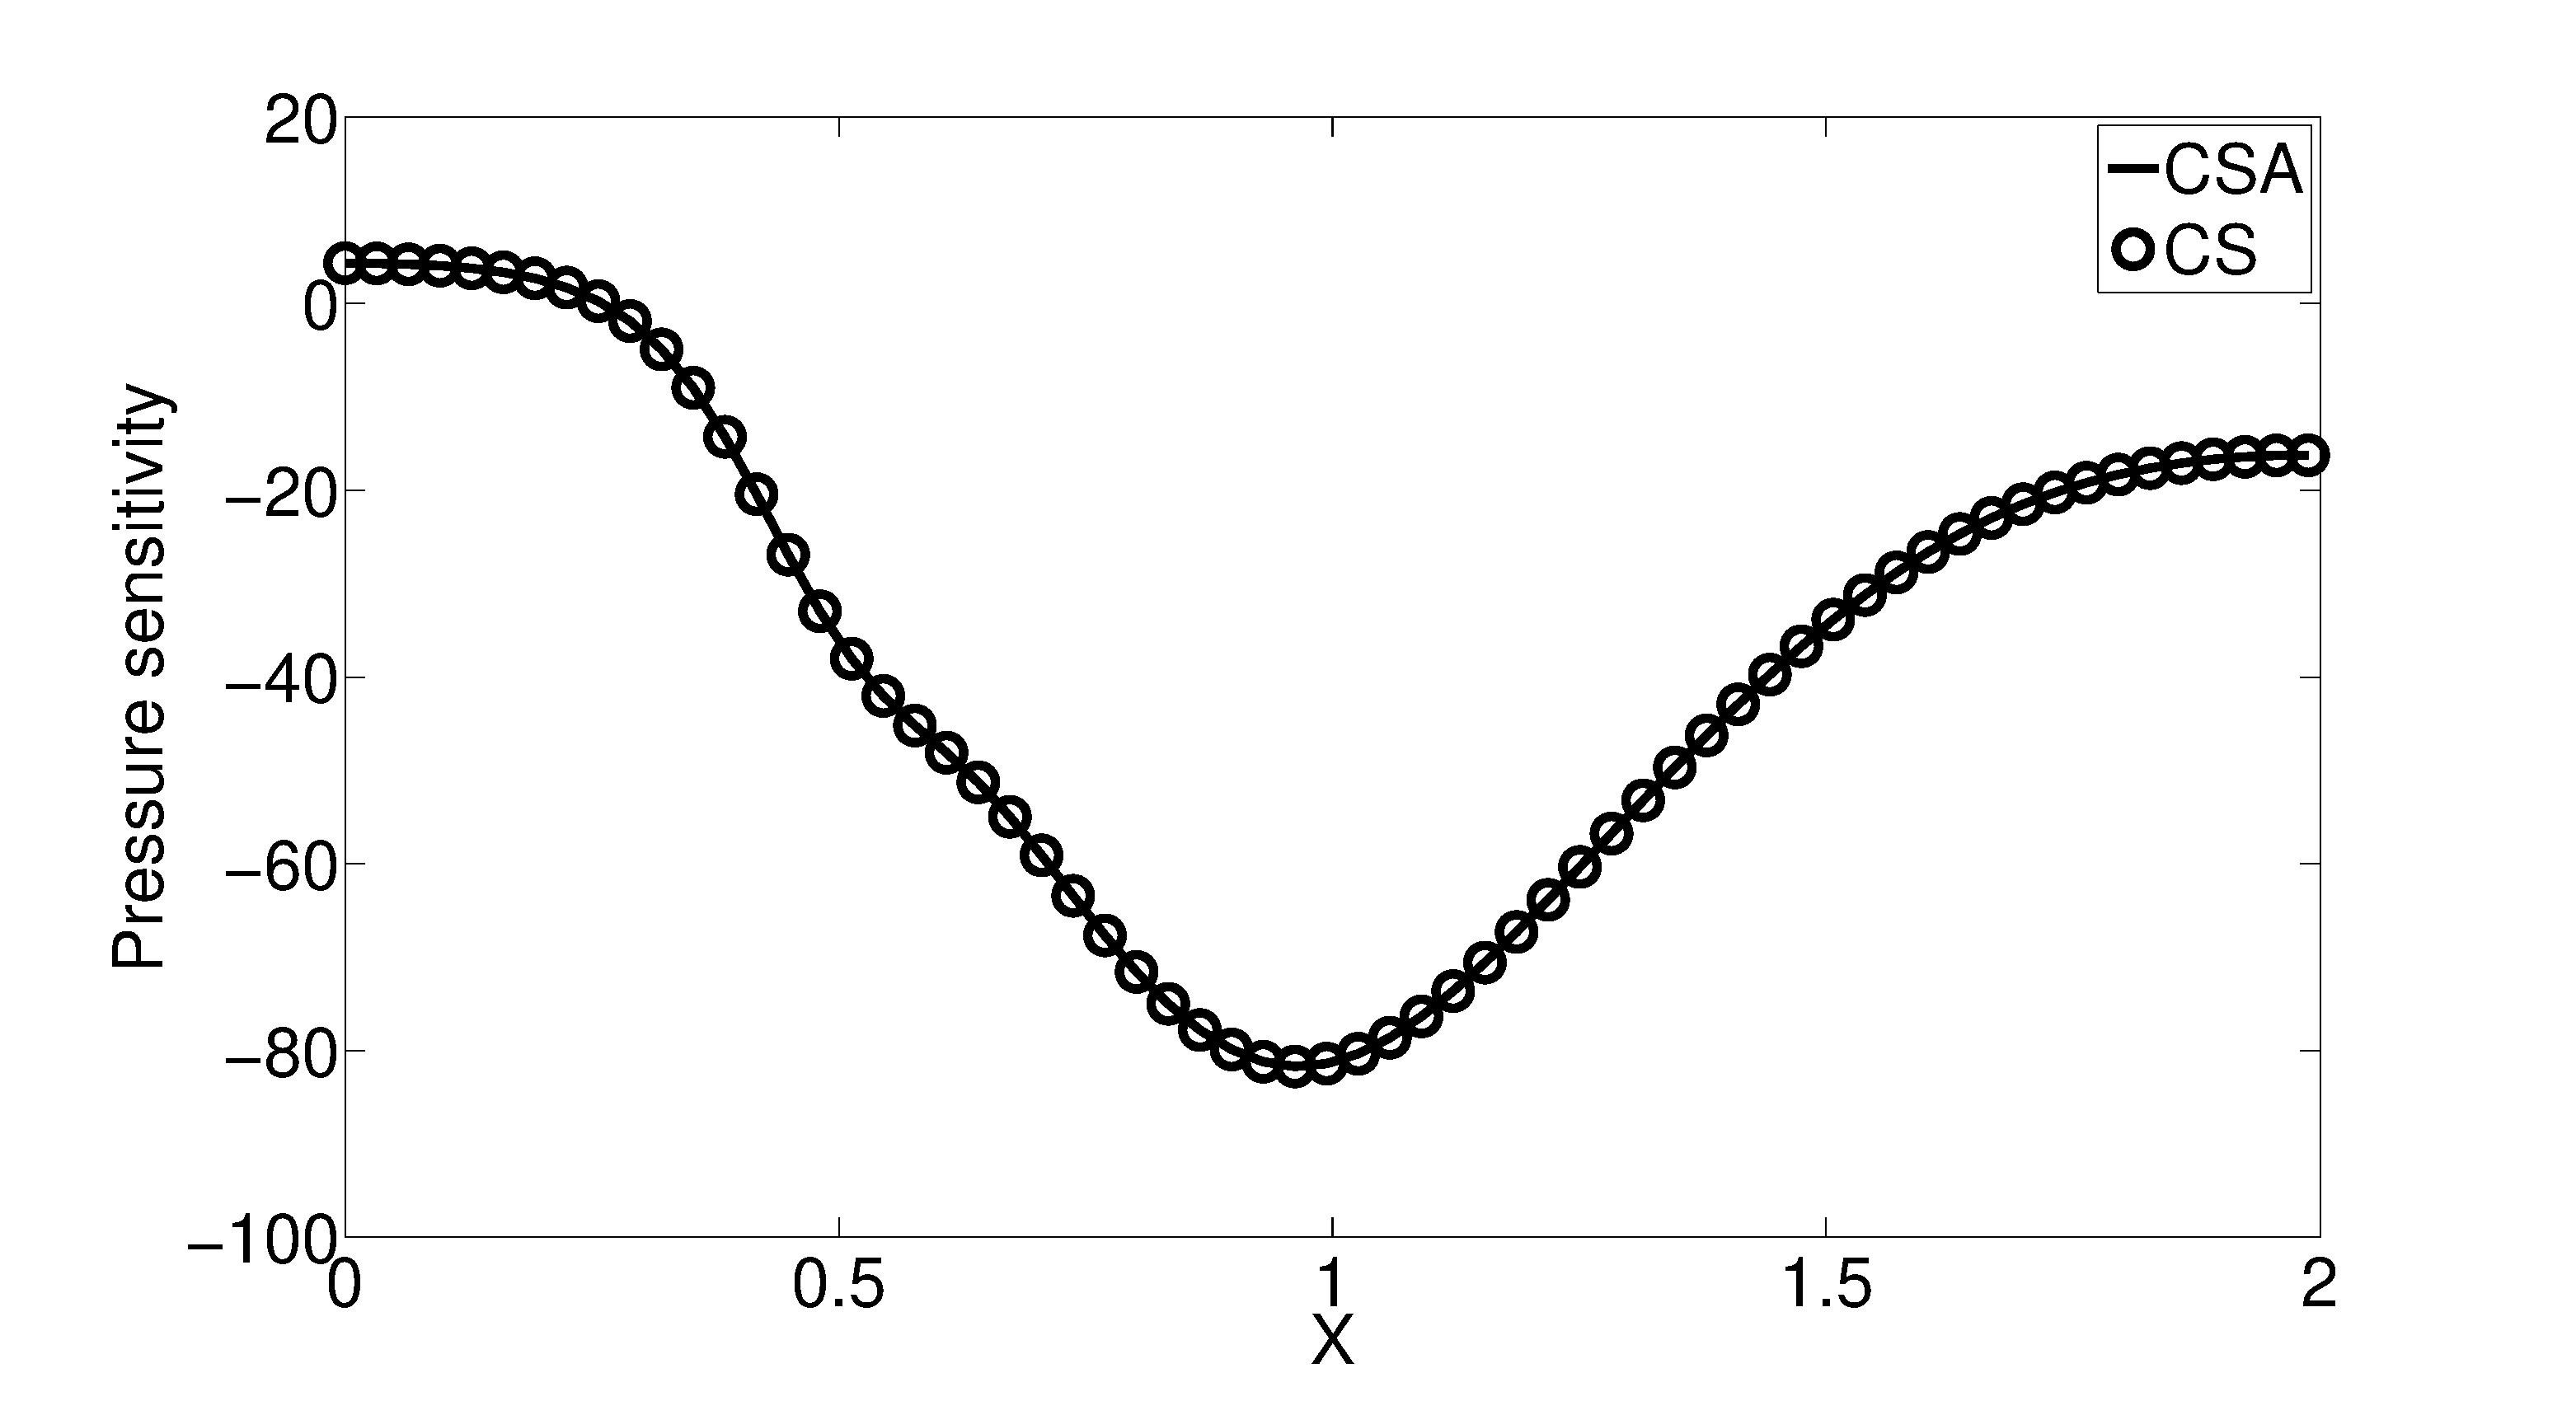
\includegraphics[height=4.0cm]{figure/cylinder/Pp025_RE1000.eps}
	}
	\\
	\subfigure[y = 0.5, Re = 100]
	{
	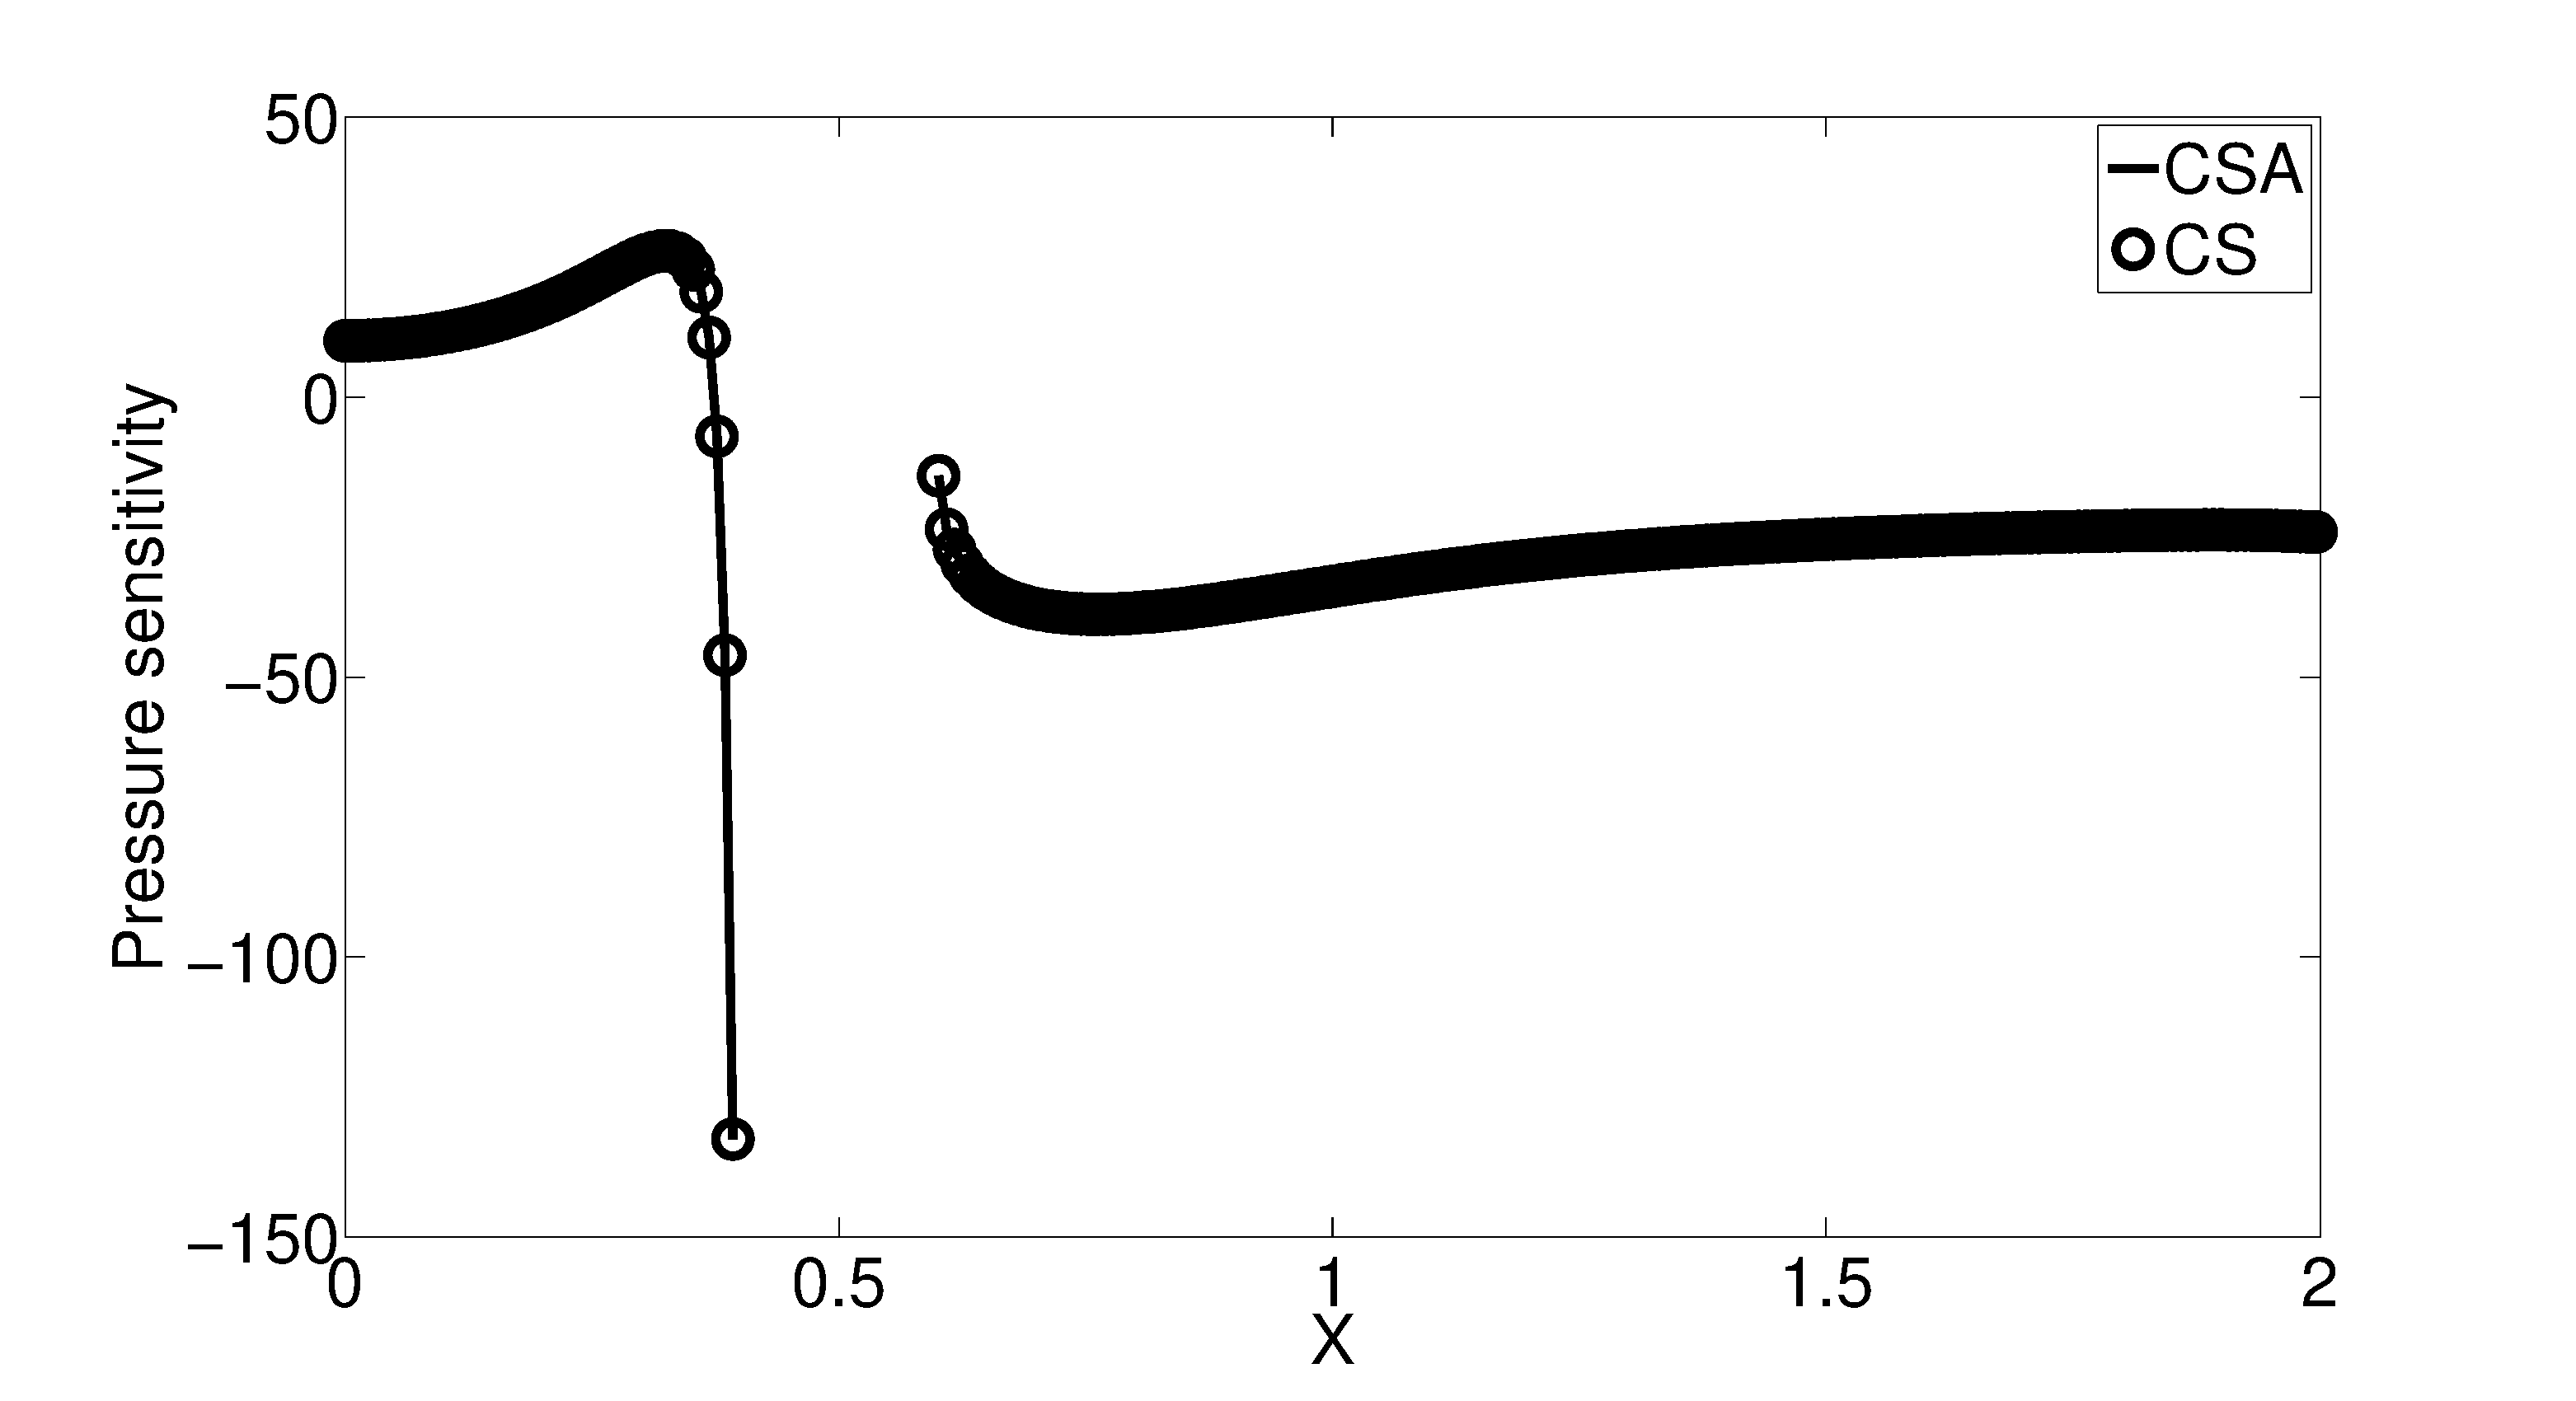
\includegraphics[height=4.0cm]{figure/cylinder/Pp050_RE100.eps}
	}
	\quad
	\subfigure[y = 0.5, Re = 1000]
	{
	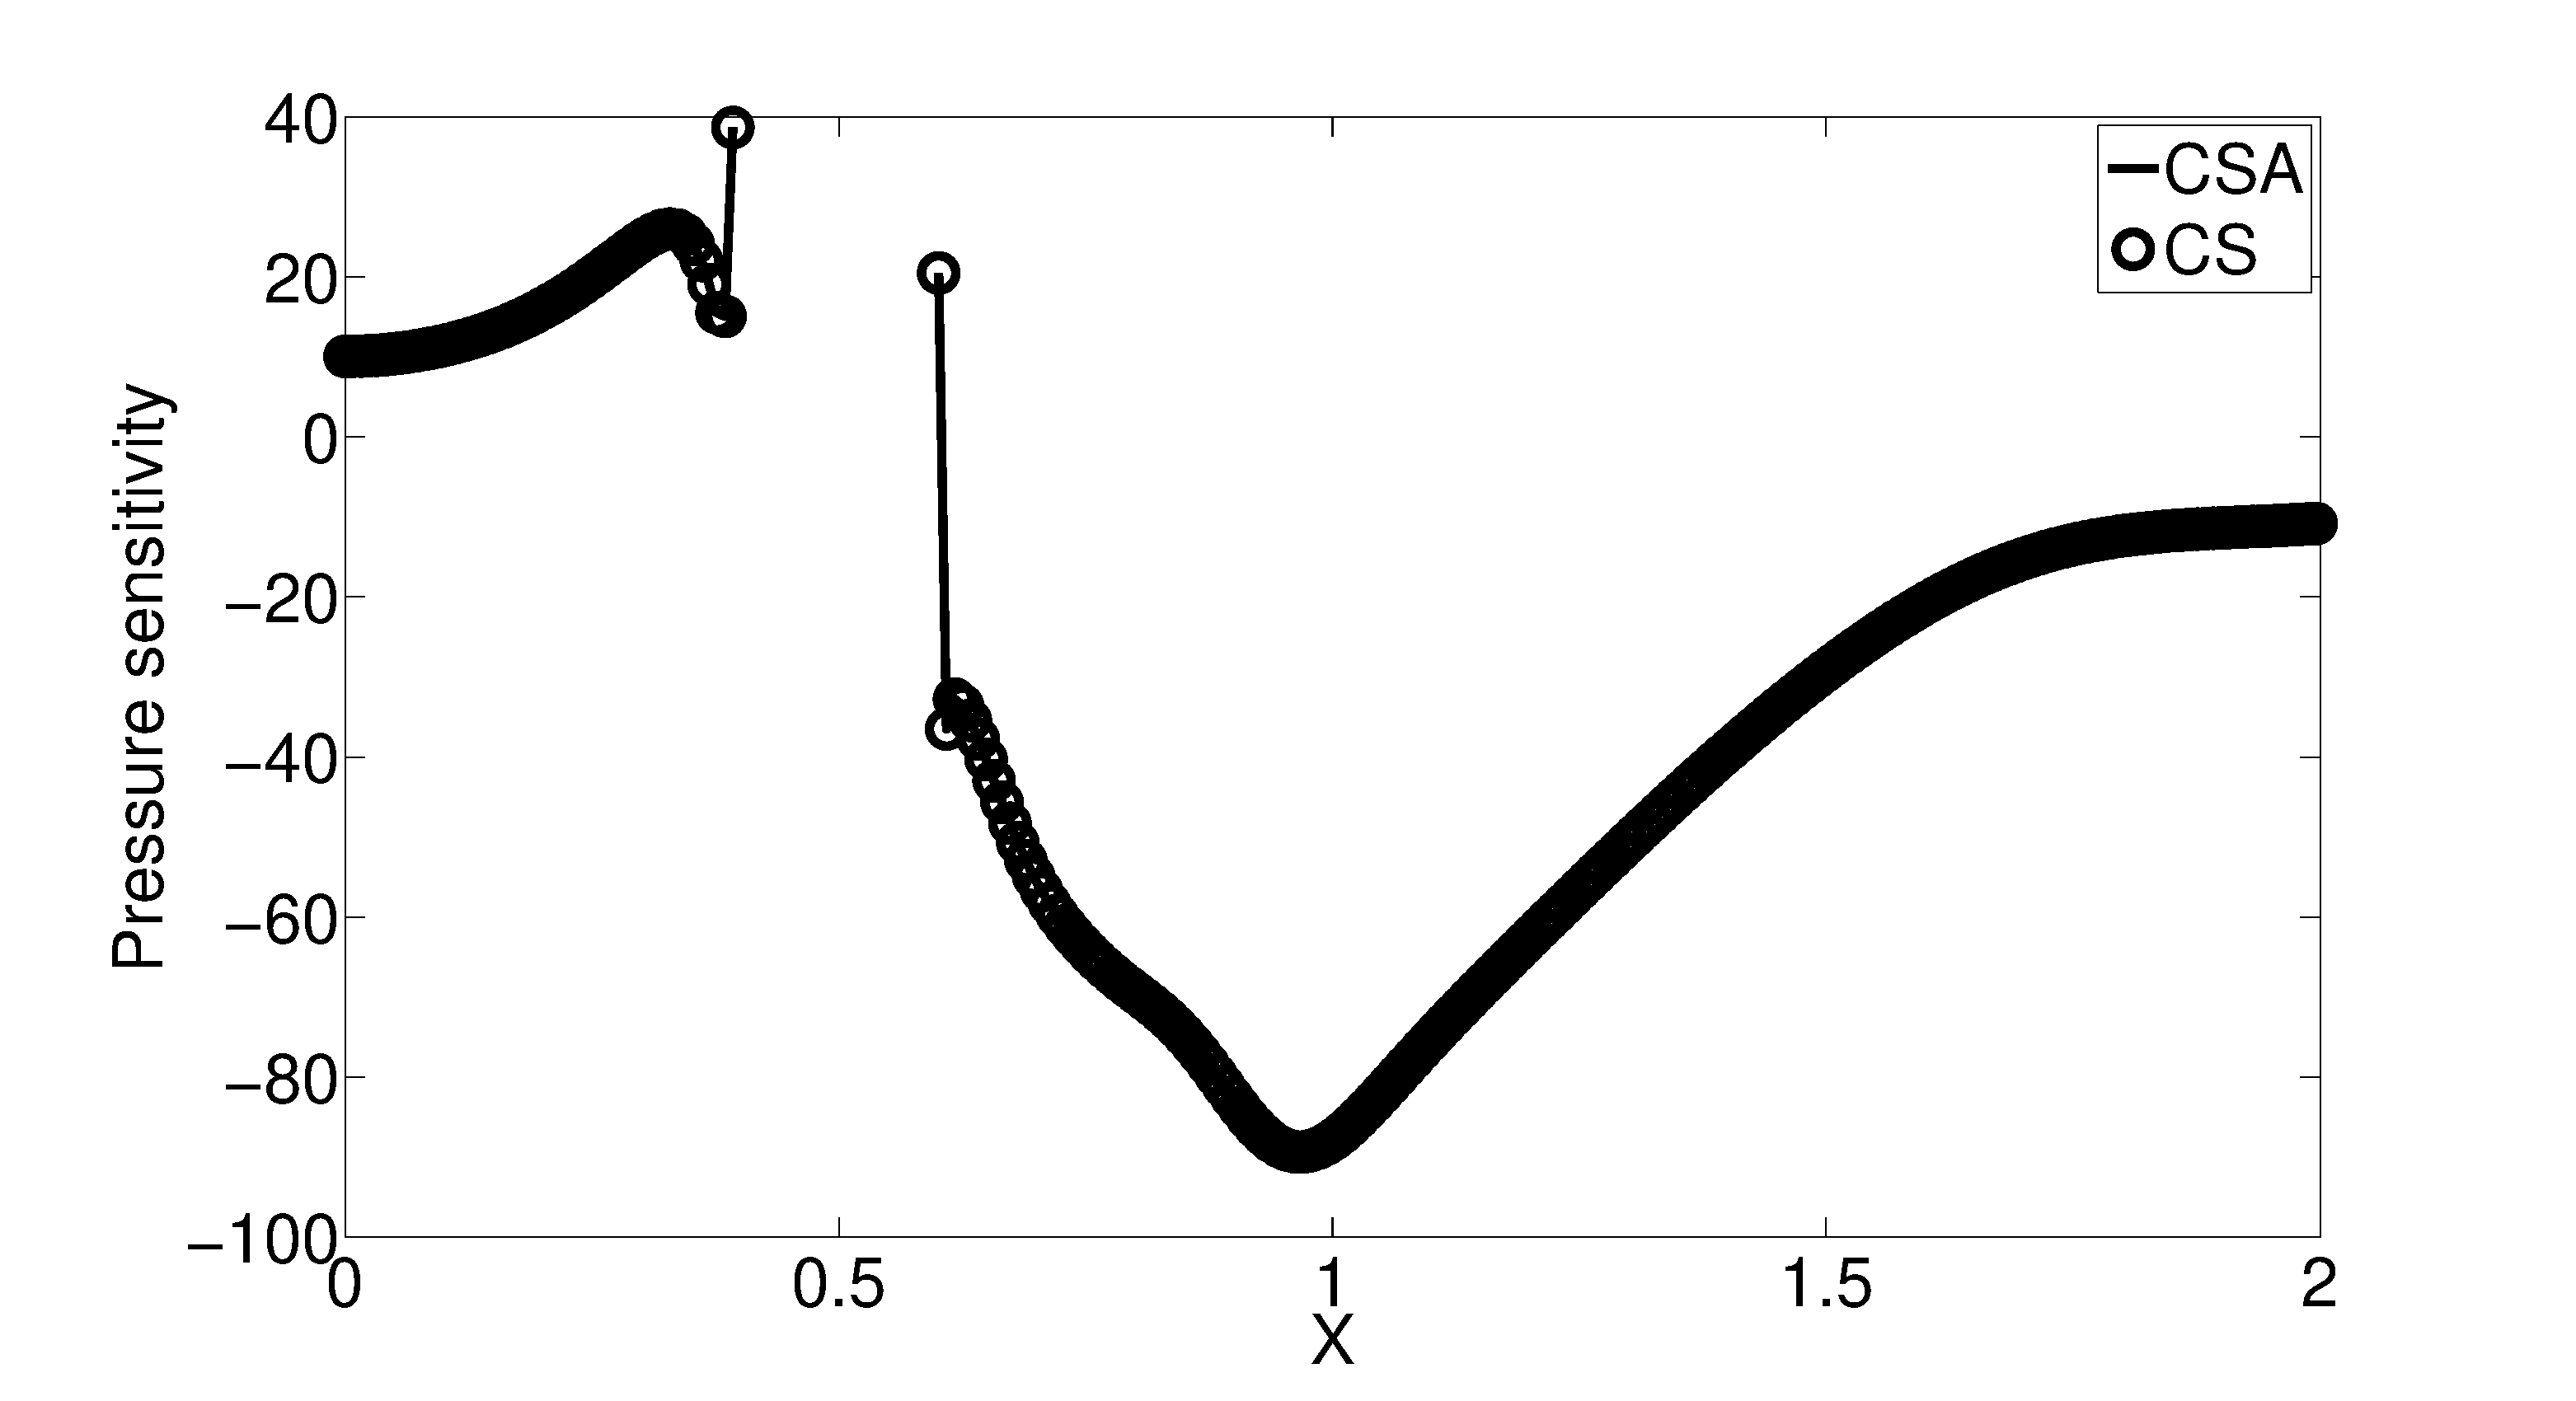
\includegraphics[height=4.0cm]{figure/cylinder/Pp050_RE1000.eps}
	}
	\\
	\subfigure[y = 0.75, Re = 100]
	{
	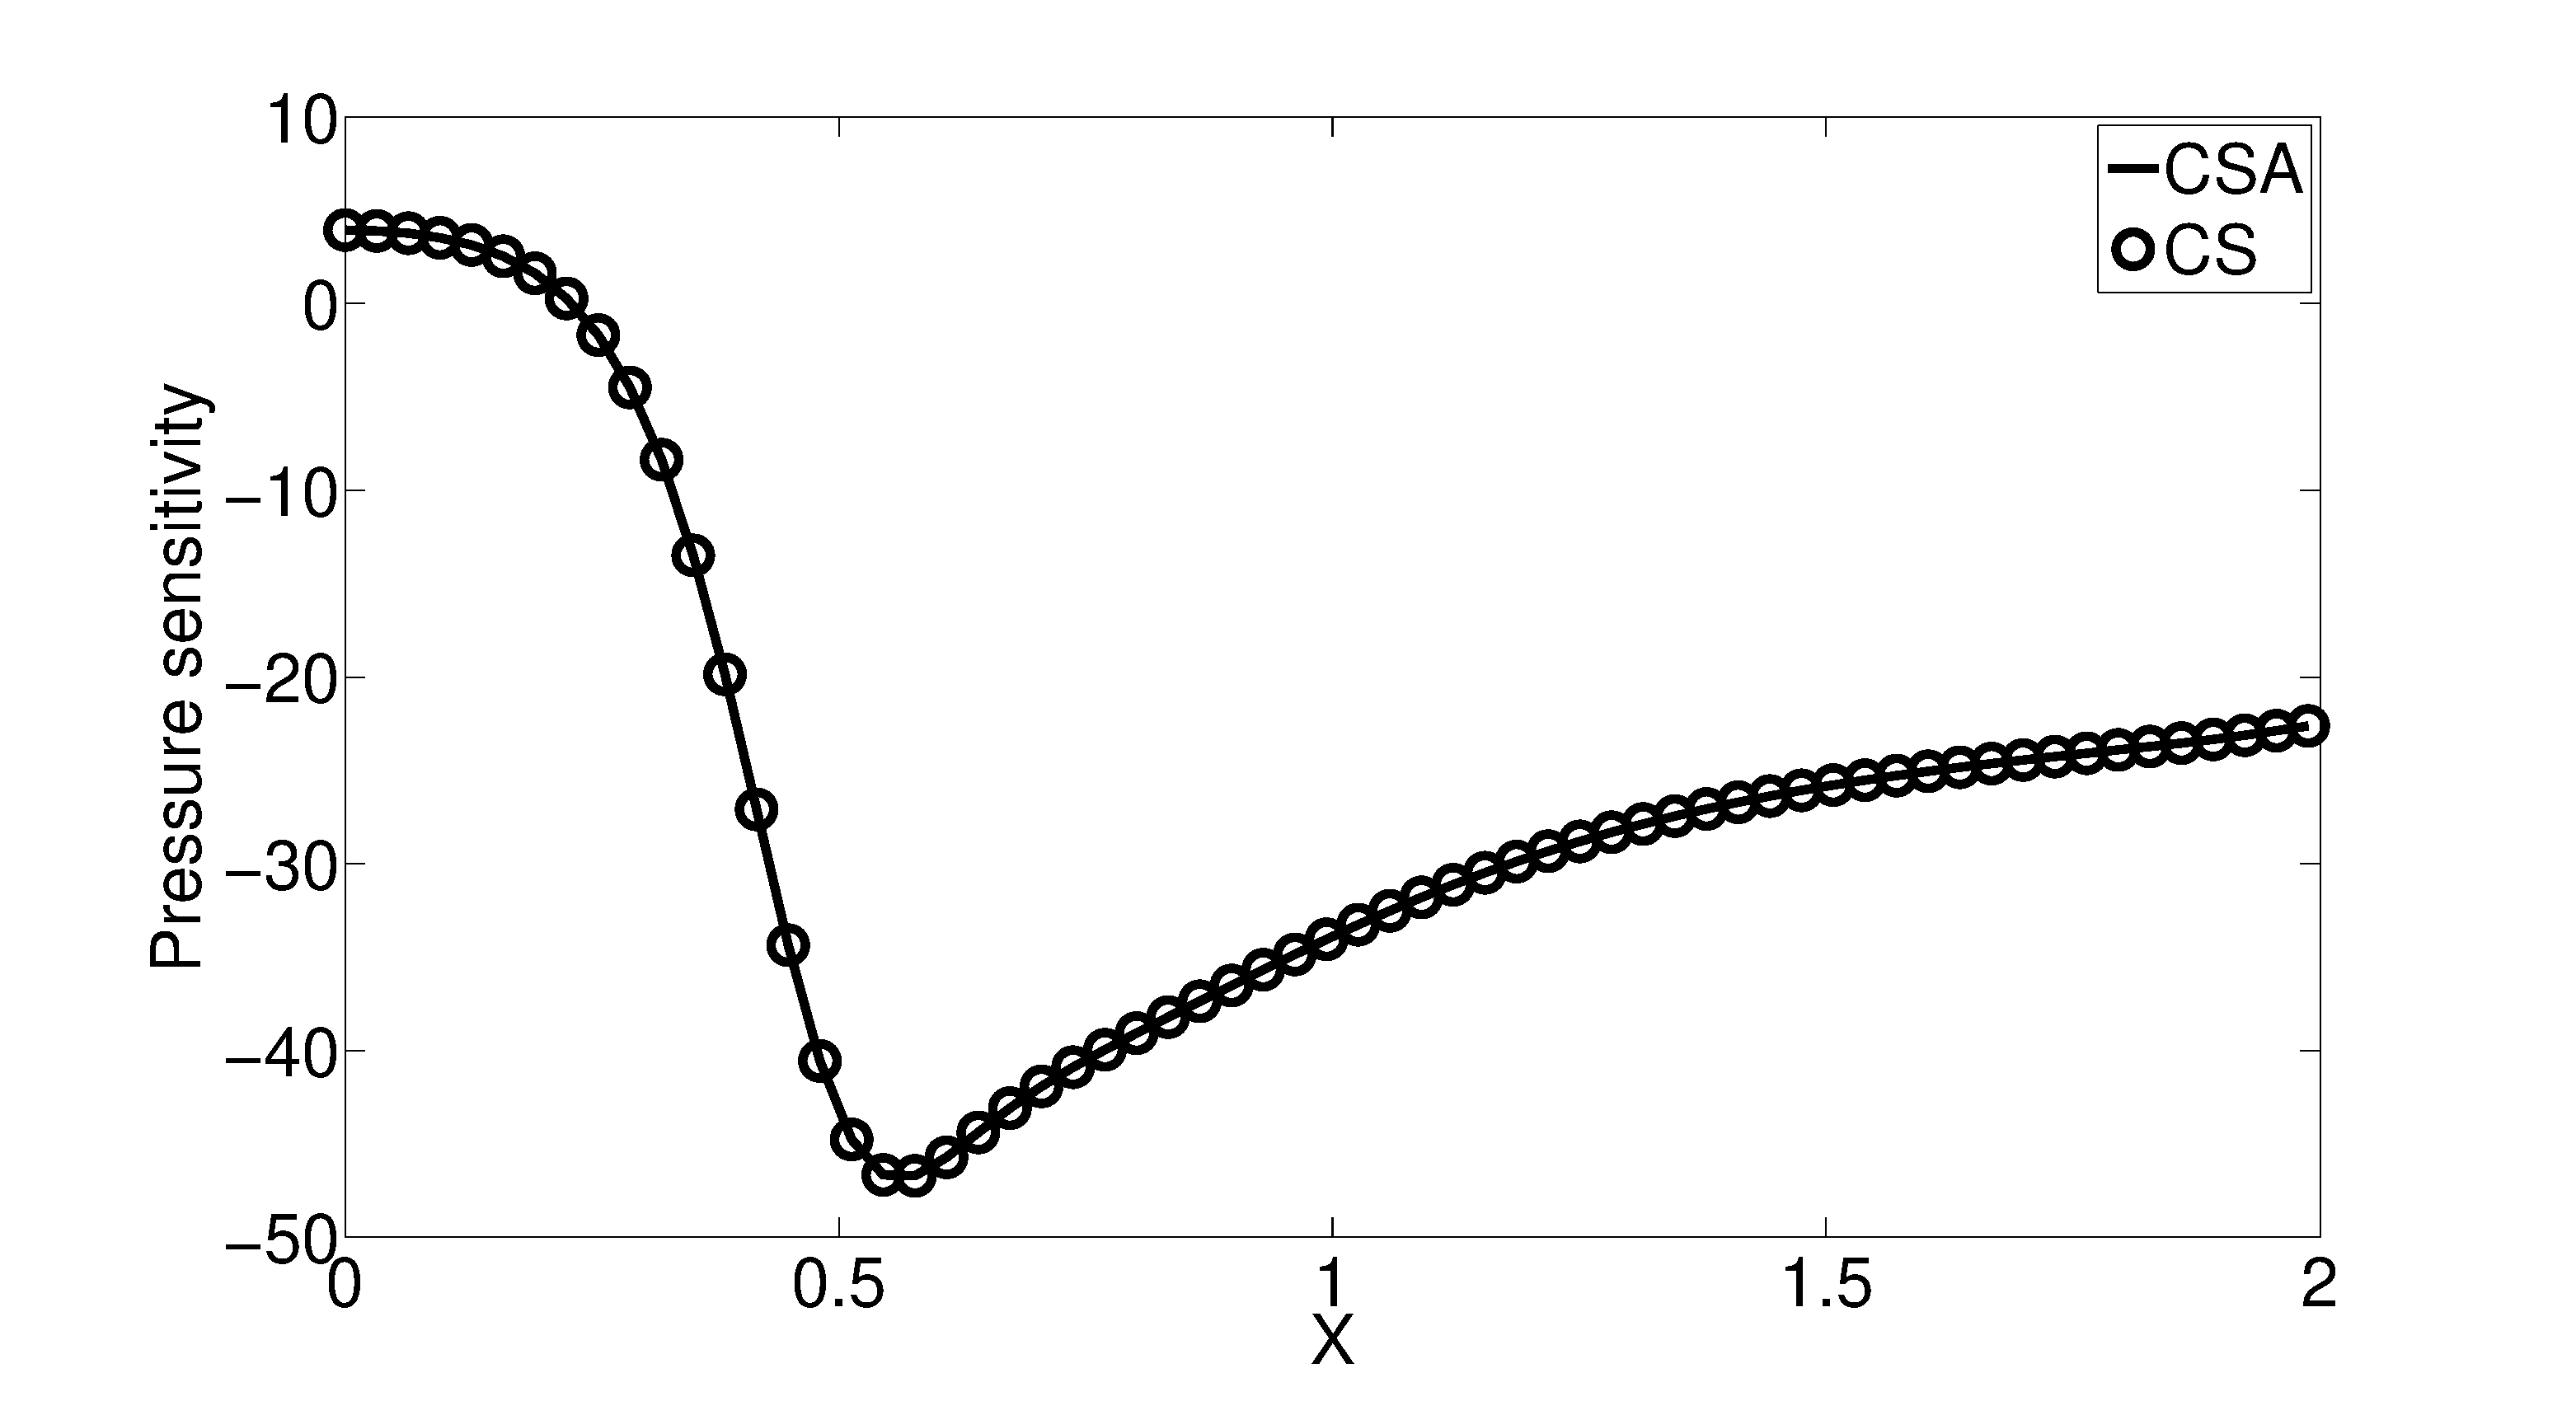
\includegraphics[height=4.0cm]{figure/cylinder/Pp075_RE100.eps}
	}
	\quad
	\subfigure[y = 0.75, Re = 1000]
	{
	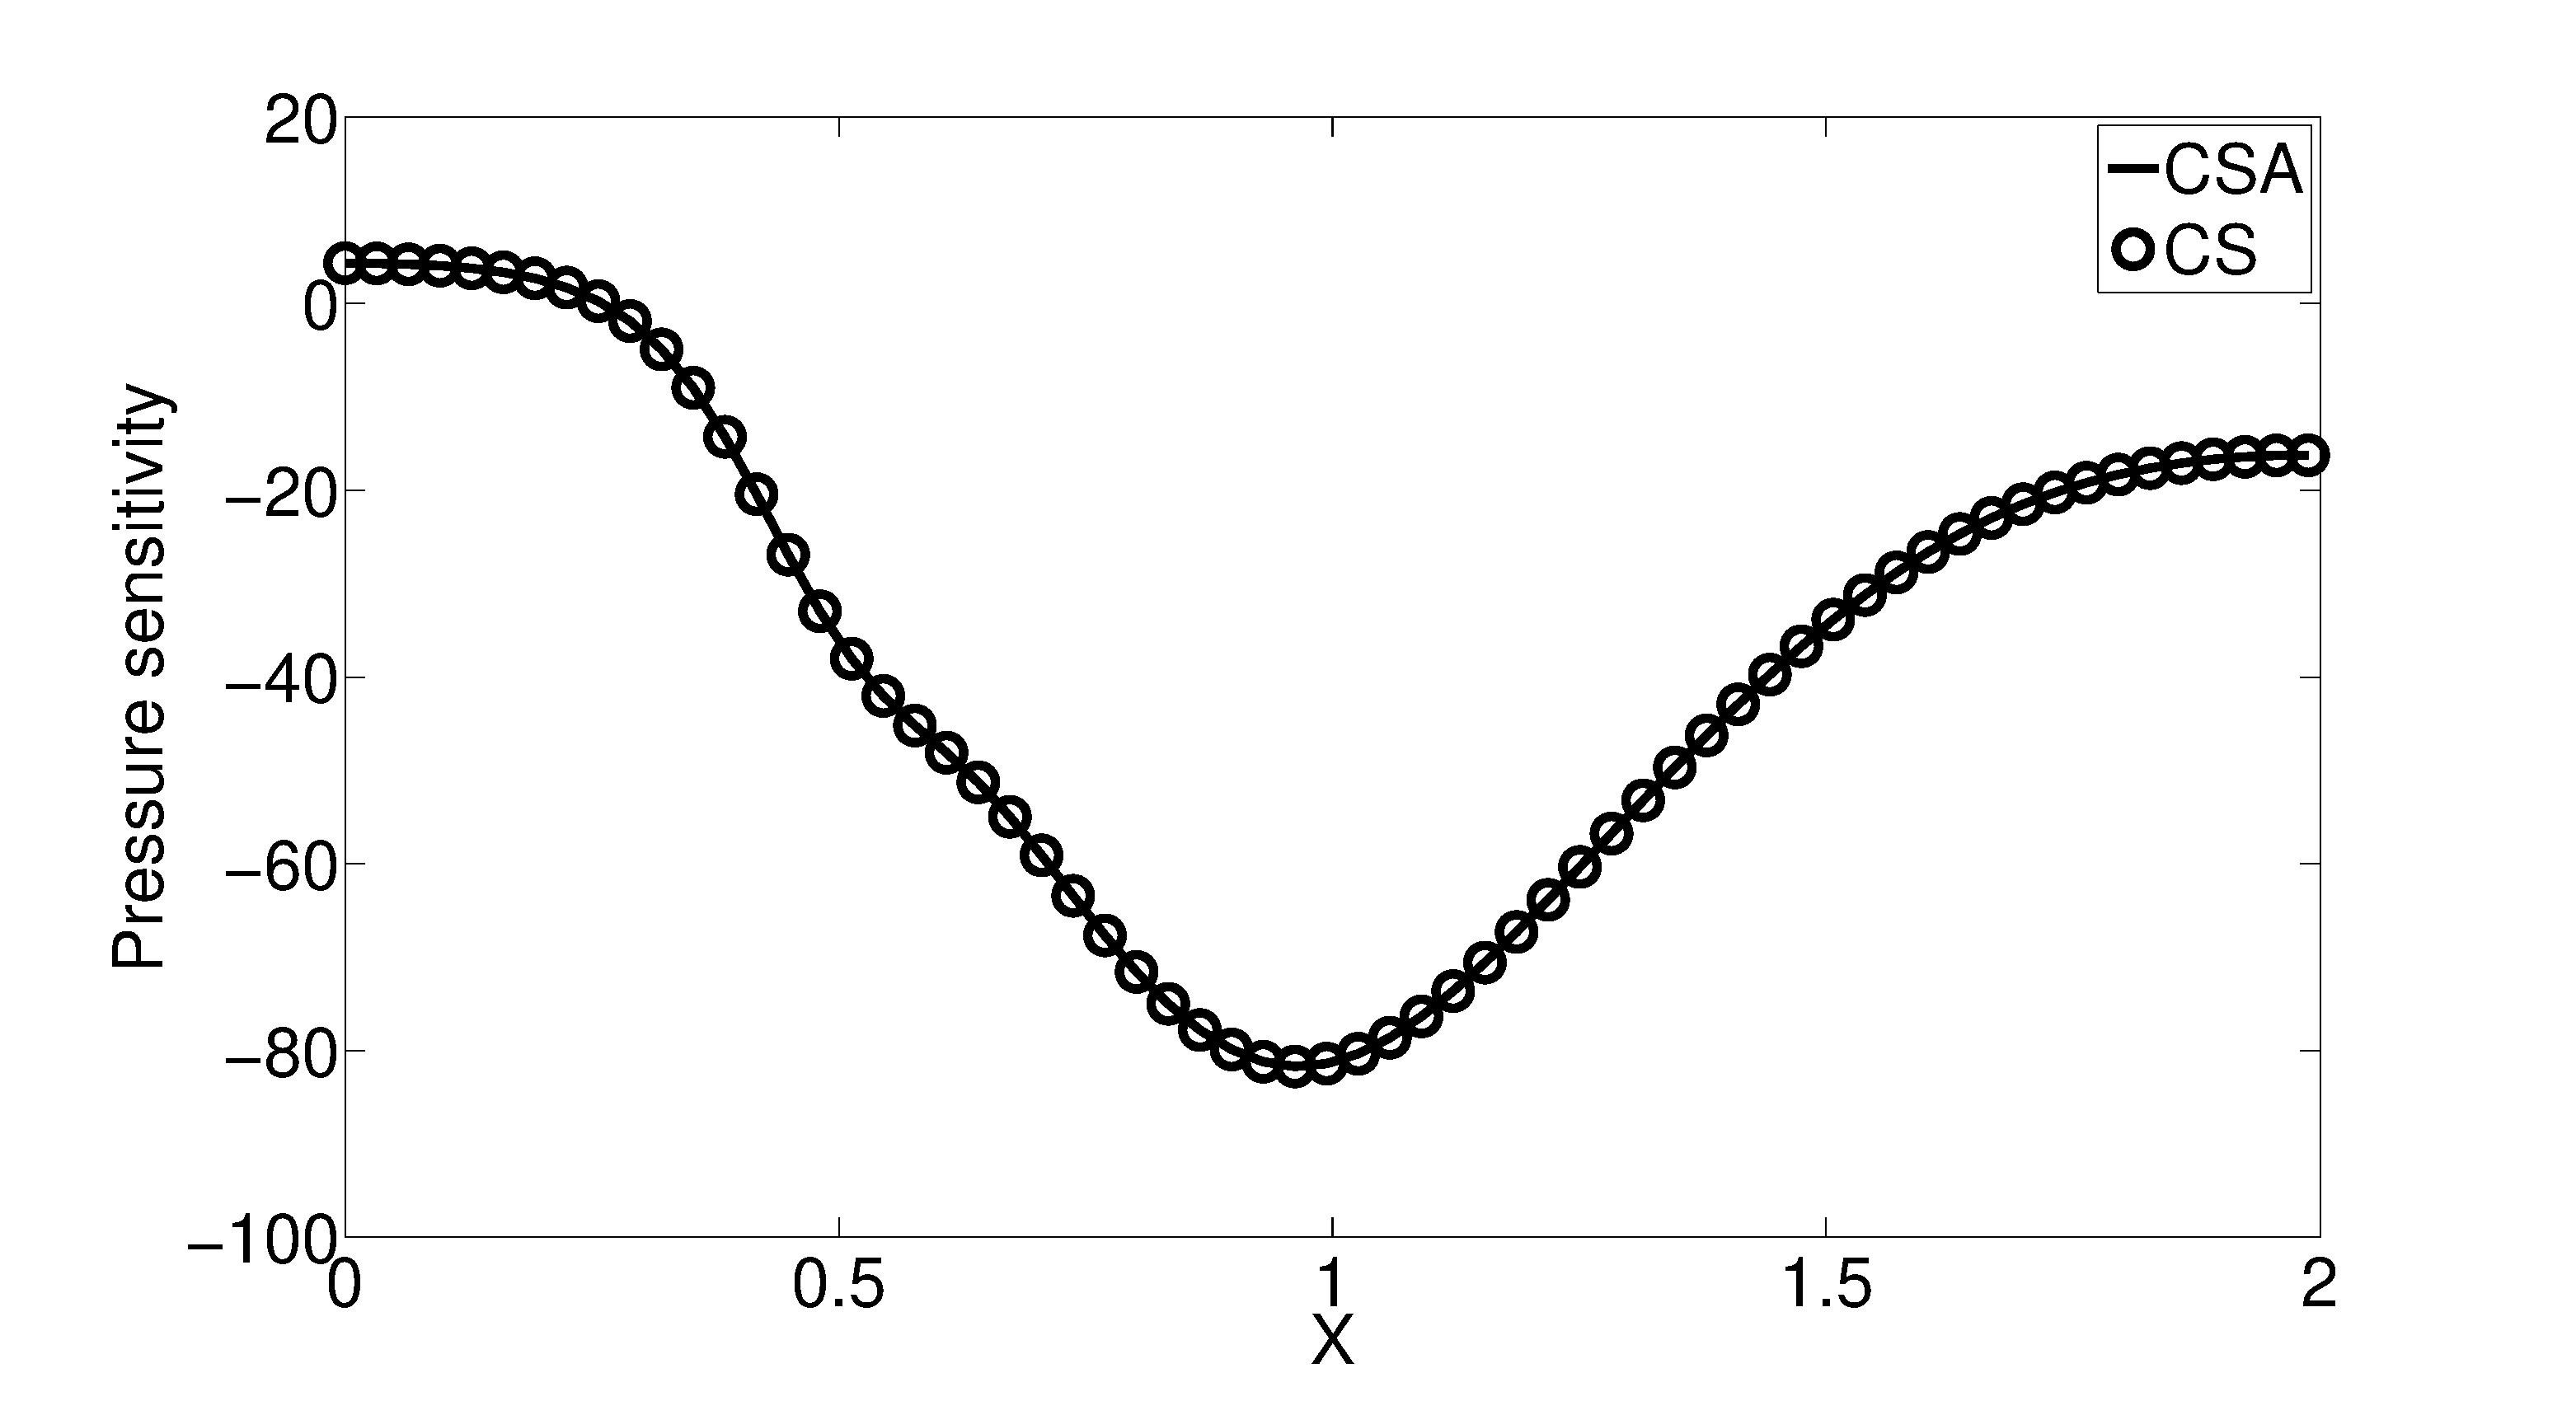
\includegraphics[height=4.0cm]{figure/cylinder/Pp075_RE1000.eps}
	}
	\caption{Pressure sensitivity to cylinder radius for different Reynolds numbers on horizontal sampling line.}
	\label{fig:cylinderPressureSensitivity}
\end{figure}
%

%
\begin{figure}[H]
	\centering
	\subfigure[x = 0.25, Re = 100]
	{
	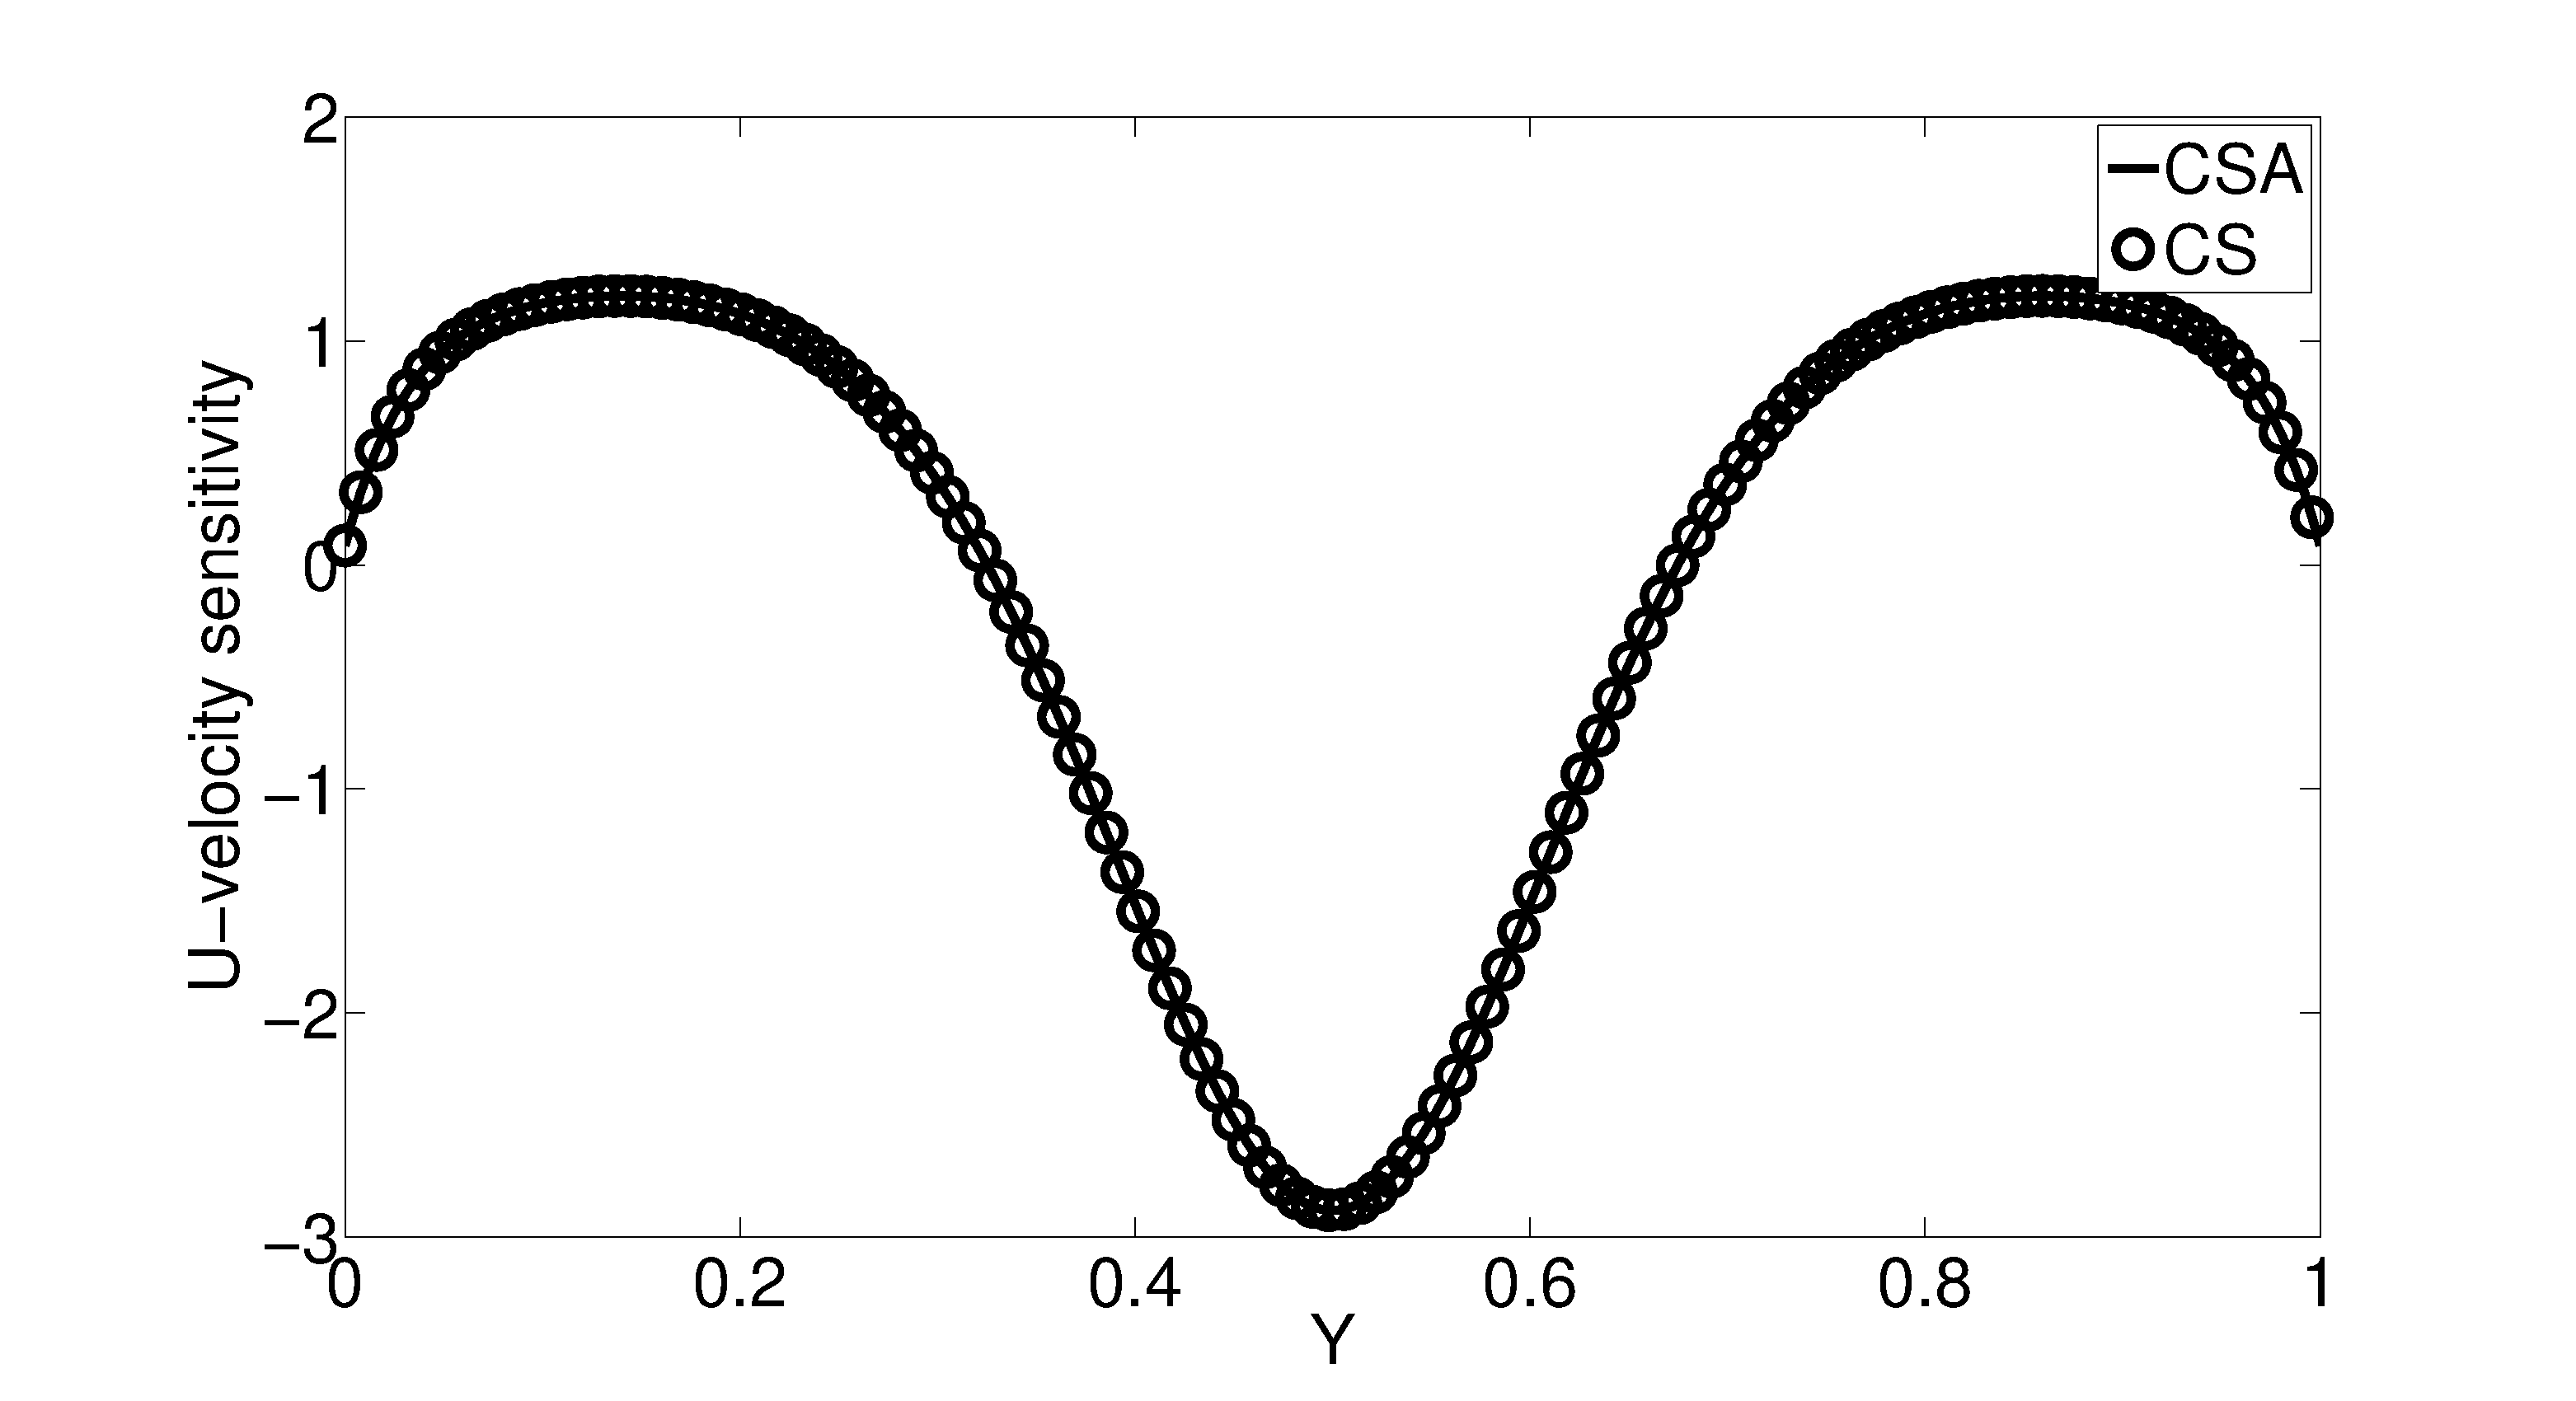
\includegraphics[height=4.0cm]{figure/cylinder/Up025_RE100.eps}
	}
	\quad
	\subfigure[x = 0.25, Re = 1000]
	{
	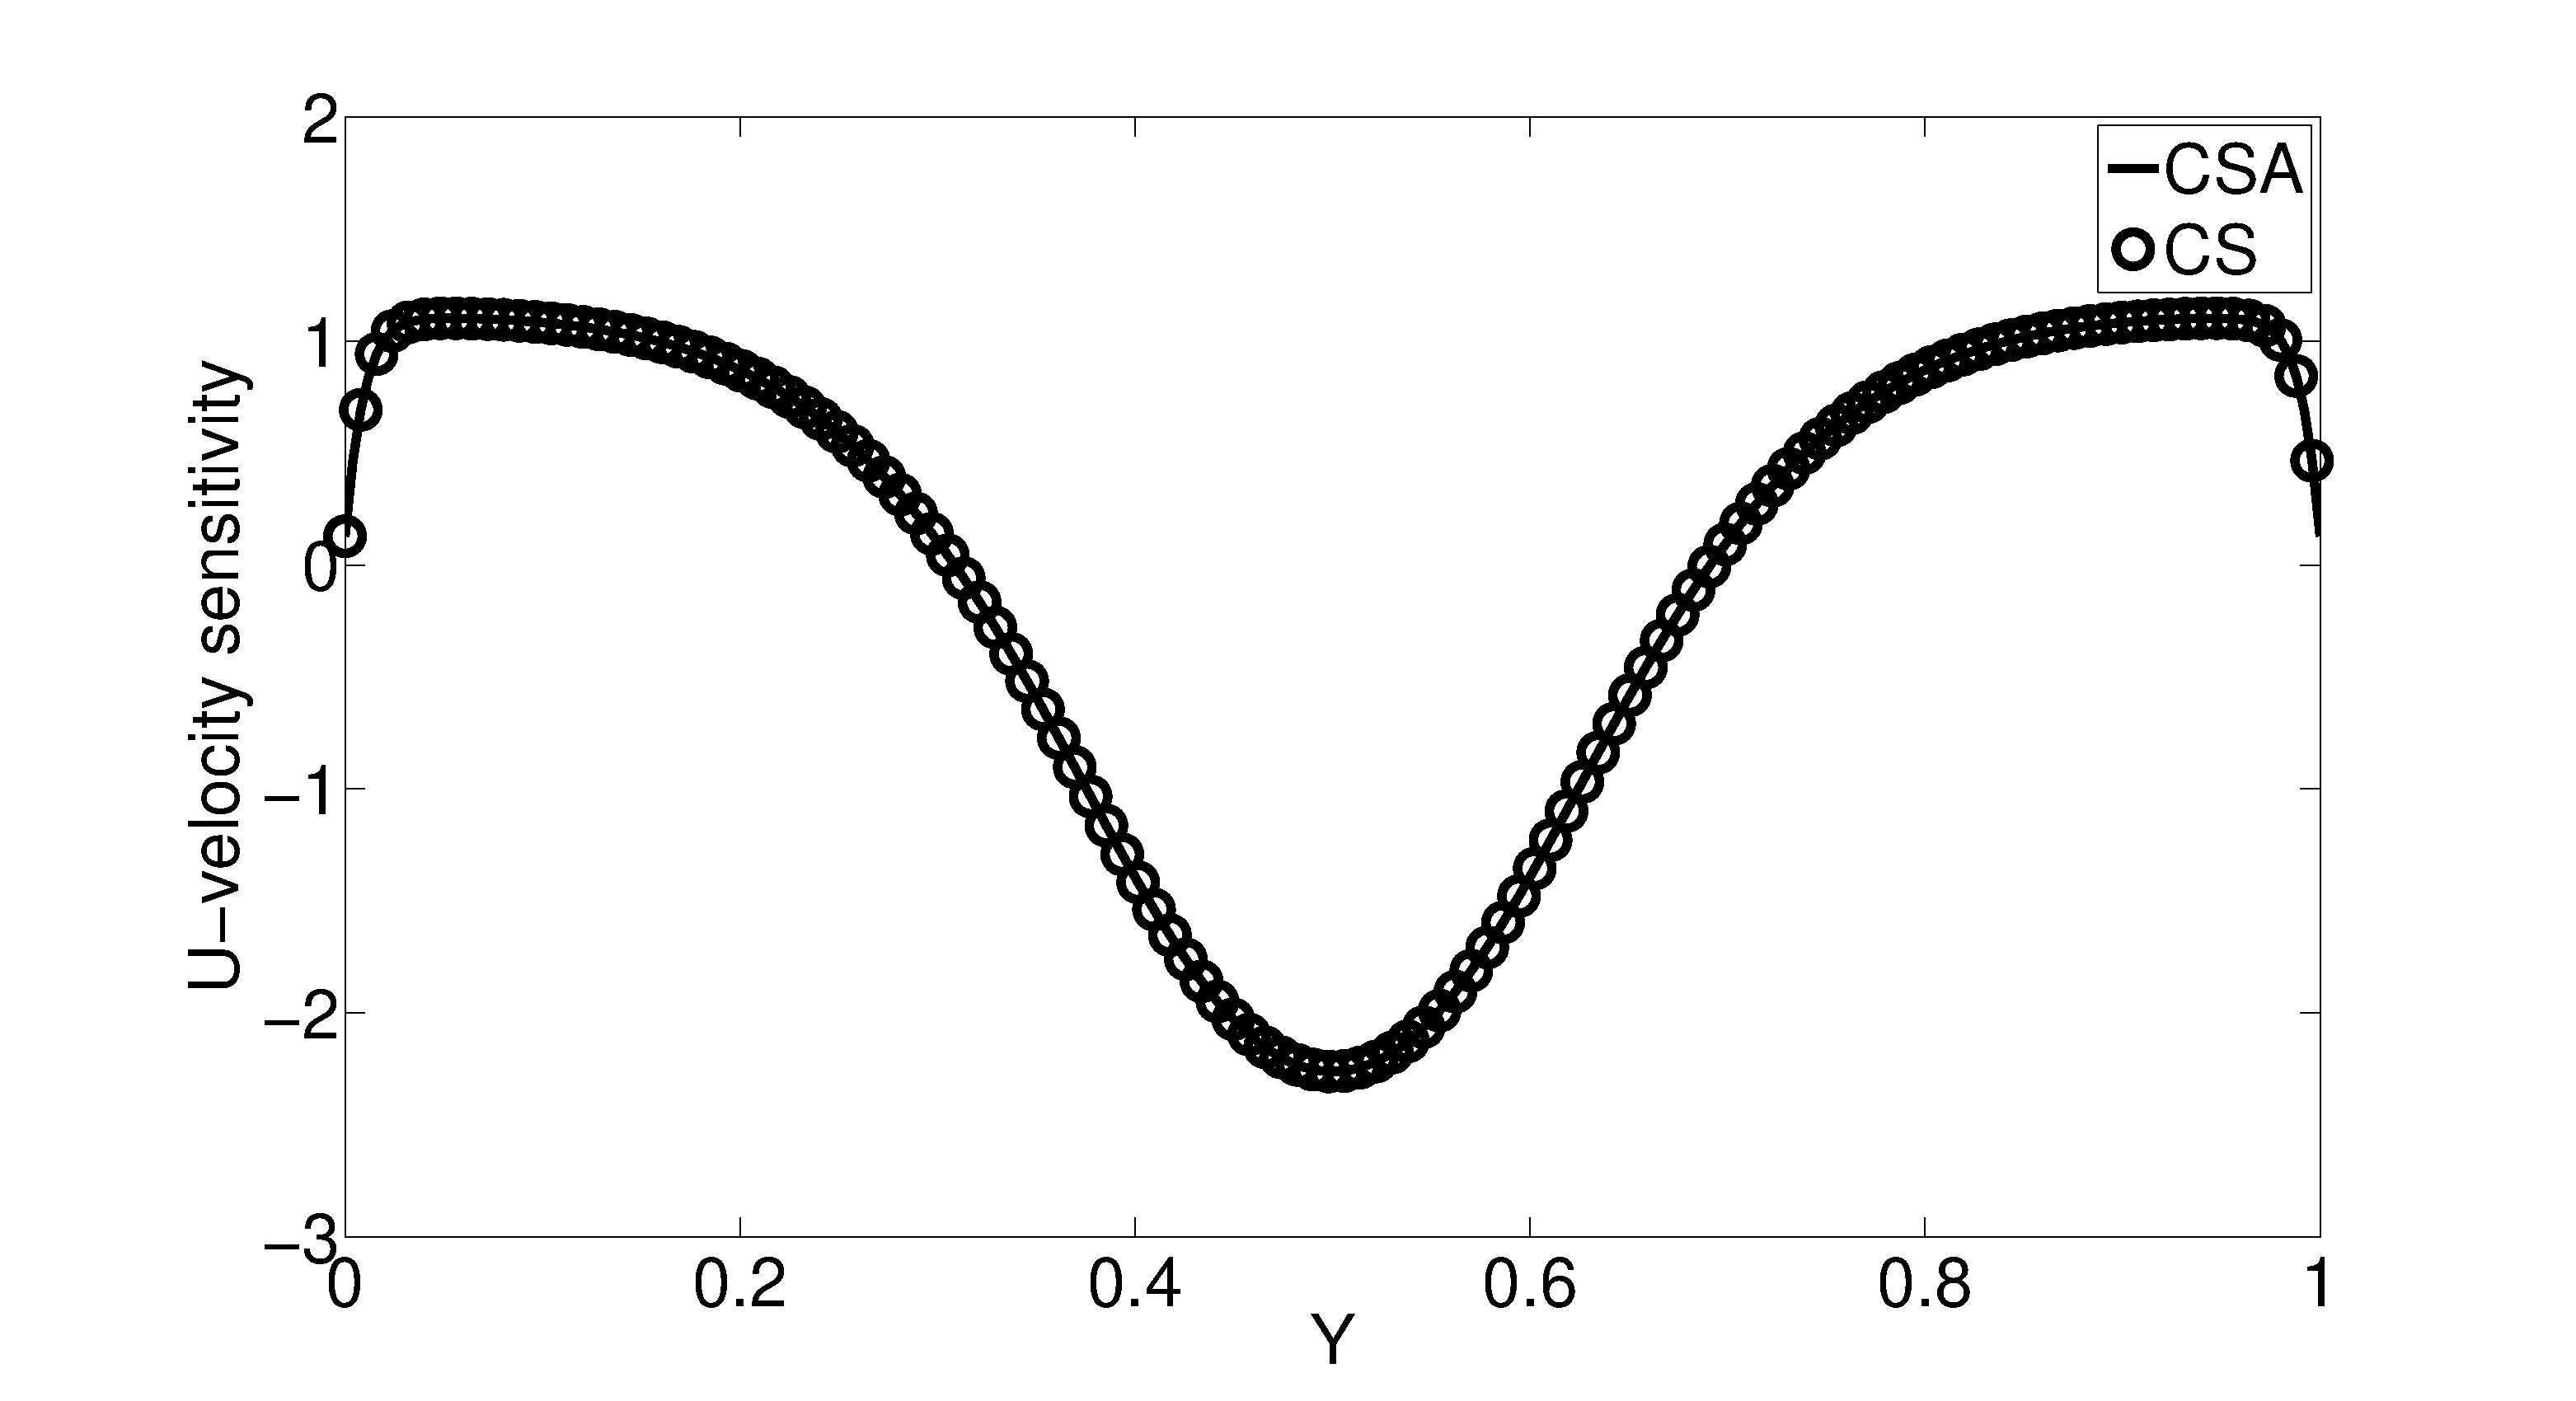
\includegraphics[height=4.0cm]{figure/cylinder/Up025_RE1000.eps}
	}
	\\
	\subfigure[x = 0.5, Re = 100]
	{
	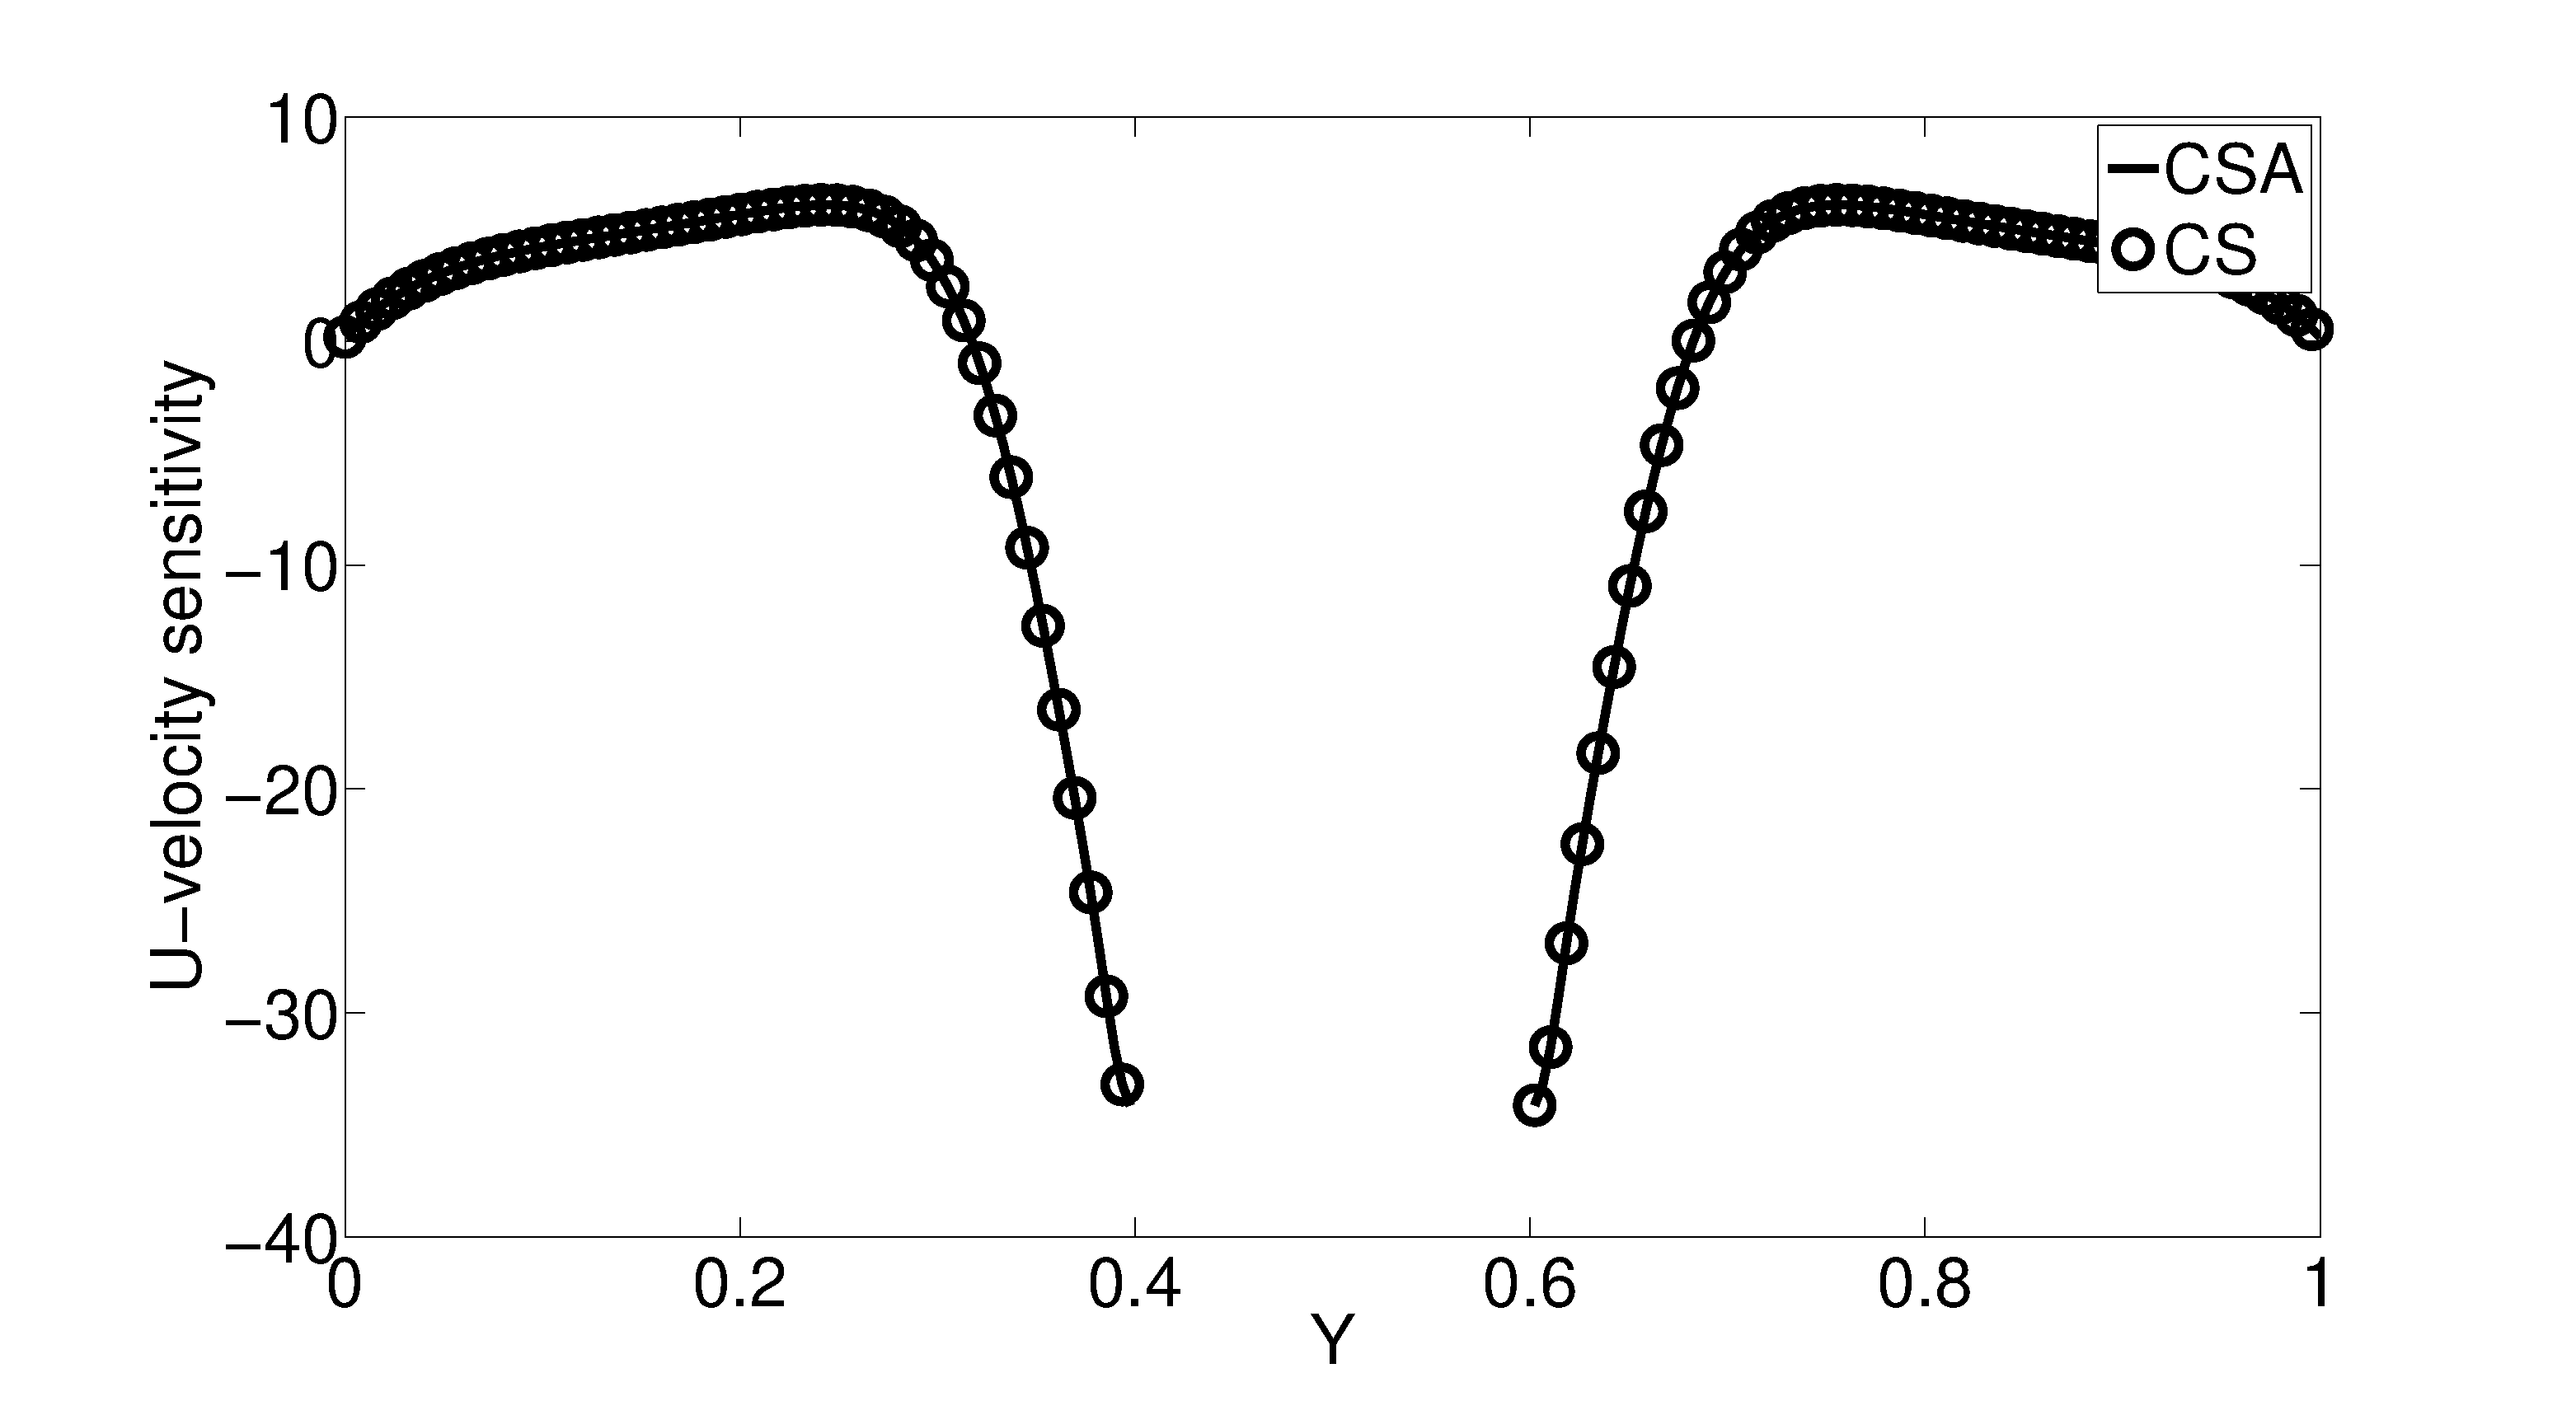
\includegraphics[height=4.0cm]{figure/cylinder/Up050_RE100.eps}
	}
	\quad
	\subfigure[x = 0.5, Re = 1000]
	{
	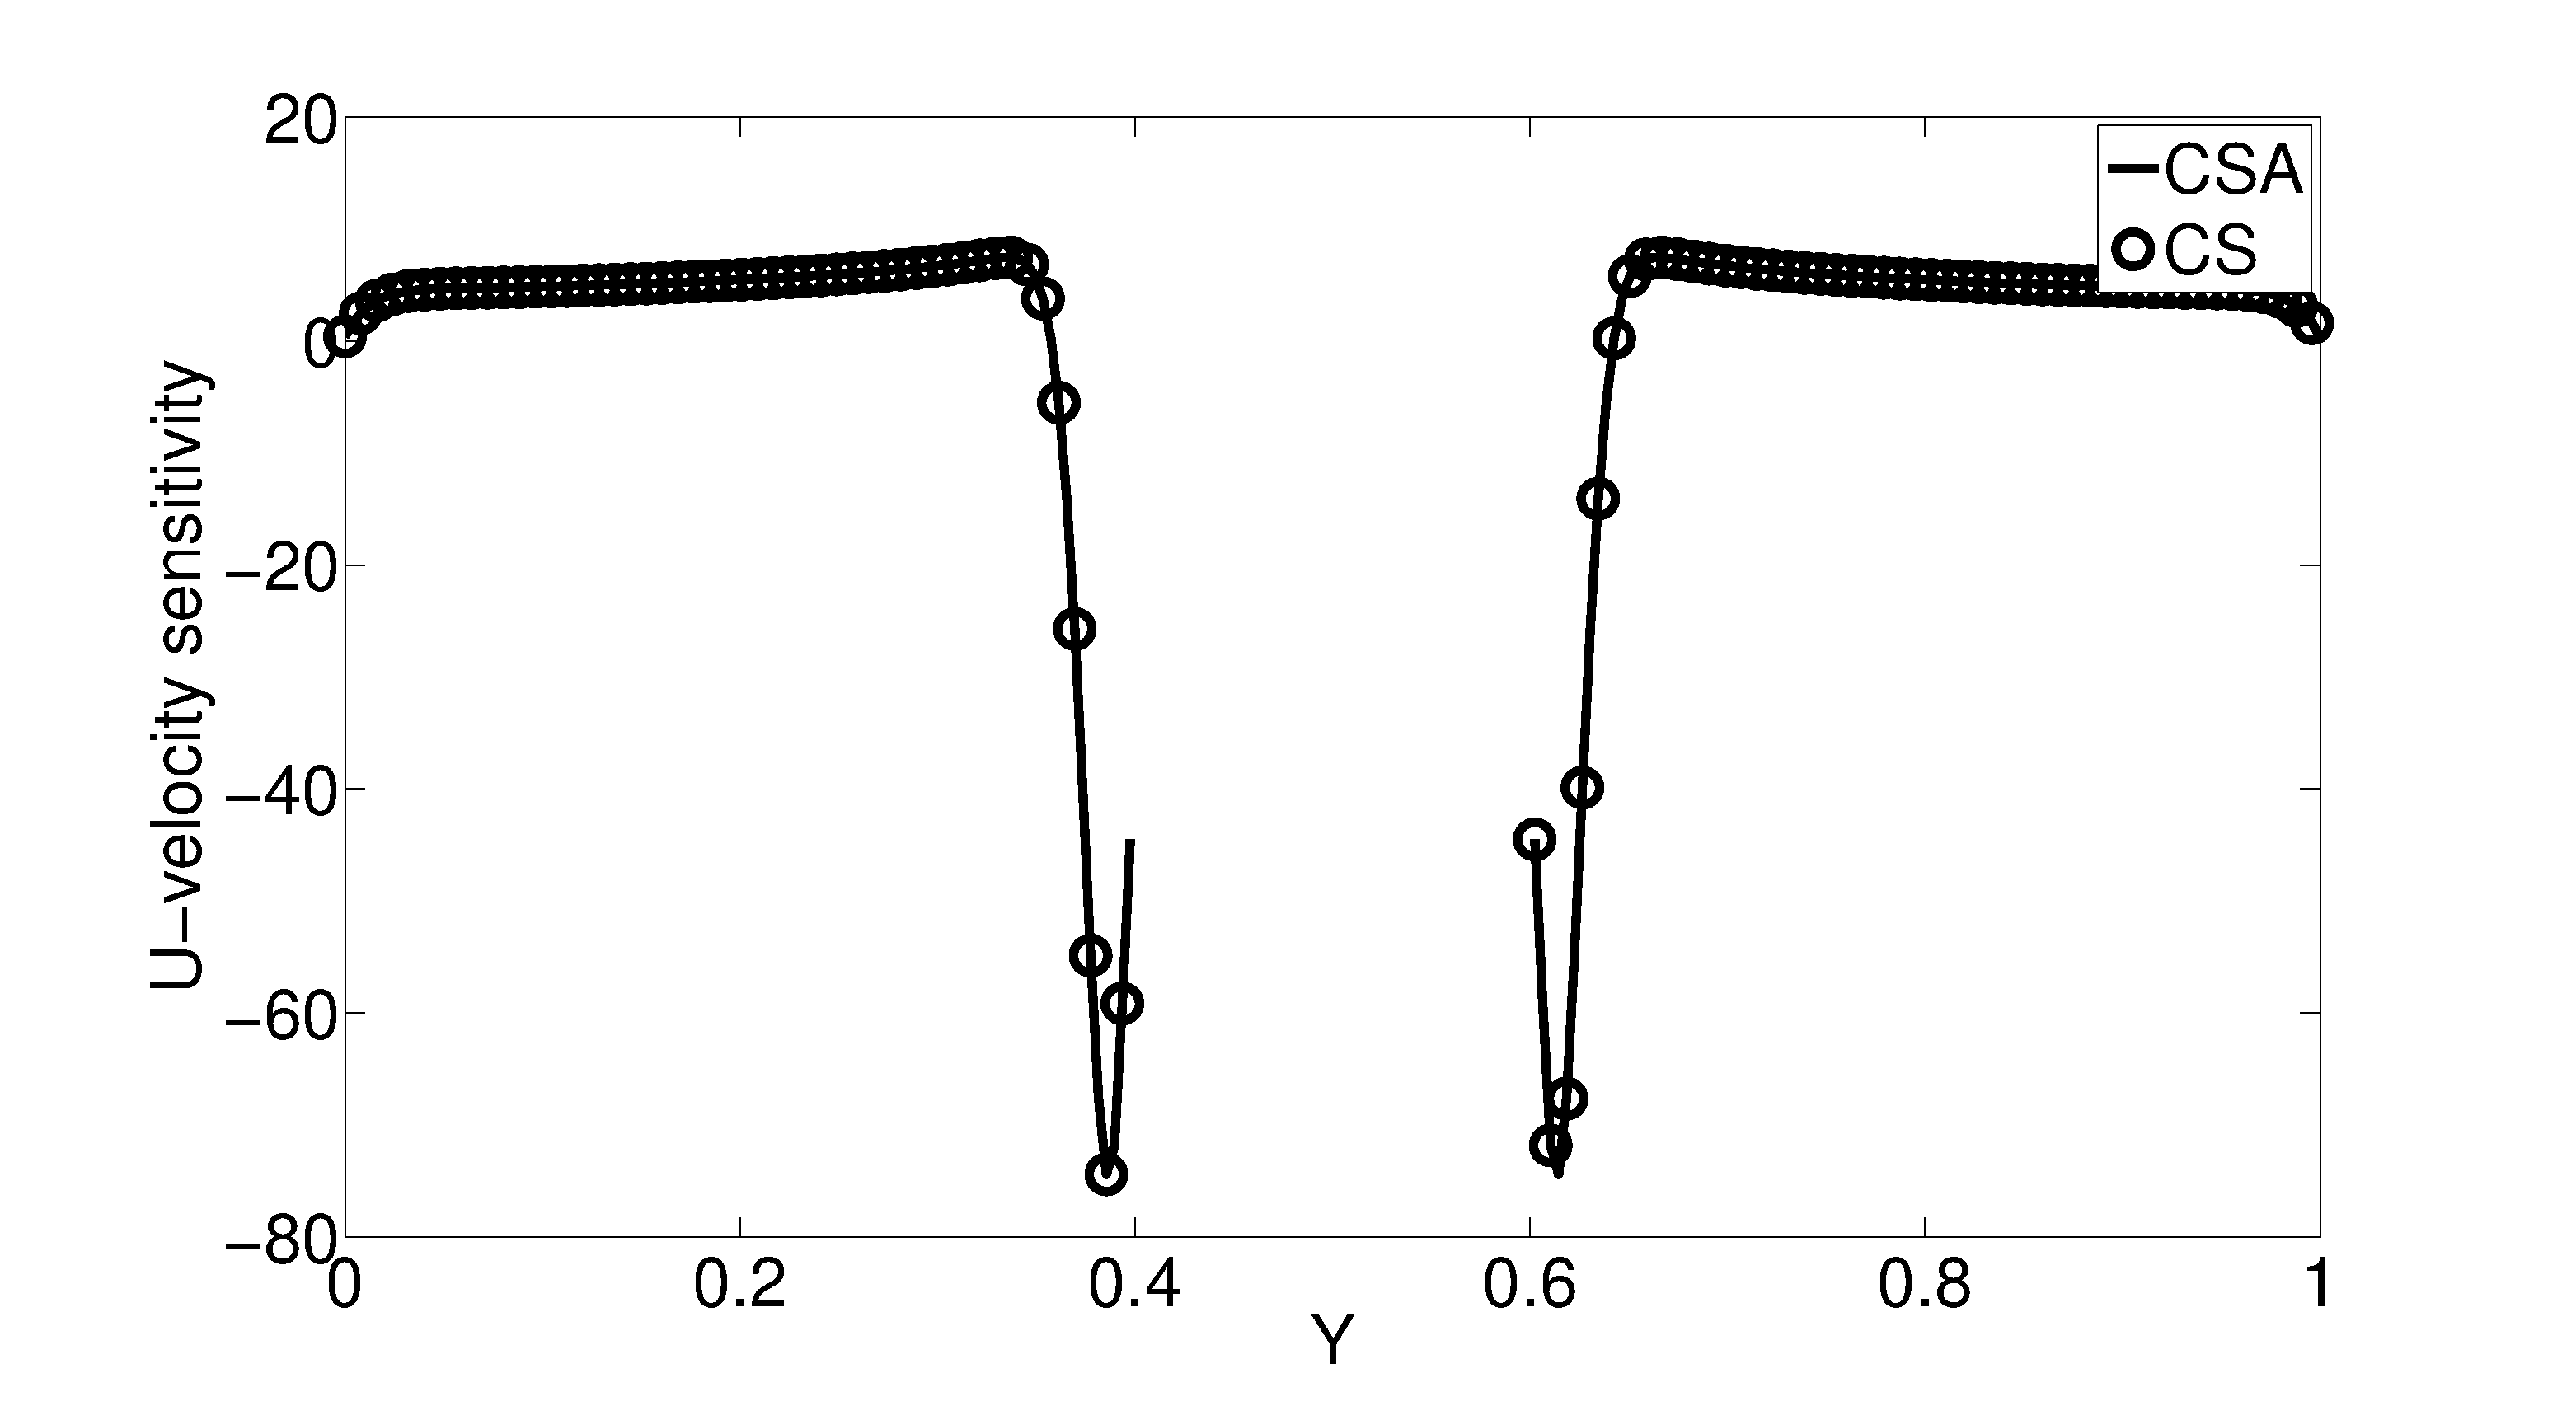
\includegraphics[height=4.0cm]{figure/cylinder/Up050_RE1000.eps}
	}
	\\
	\subfigure[x = 0.75, Re = 100]
	{
	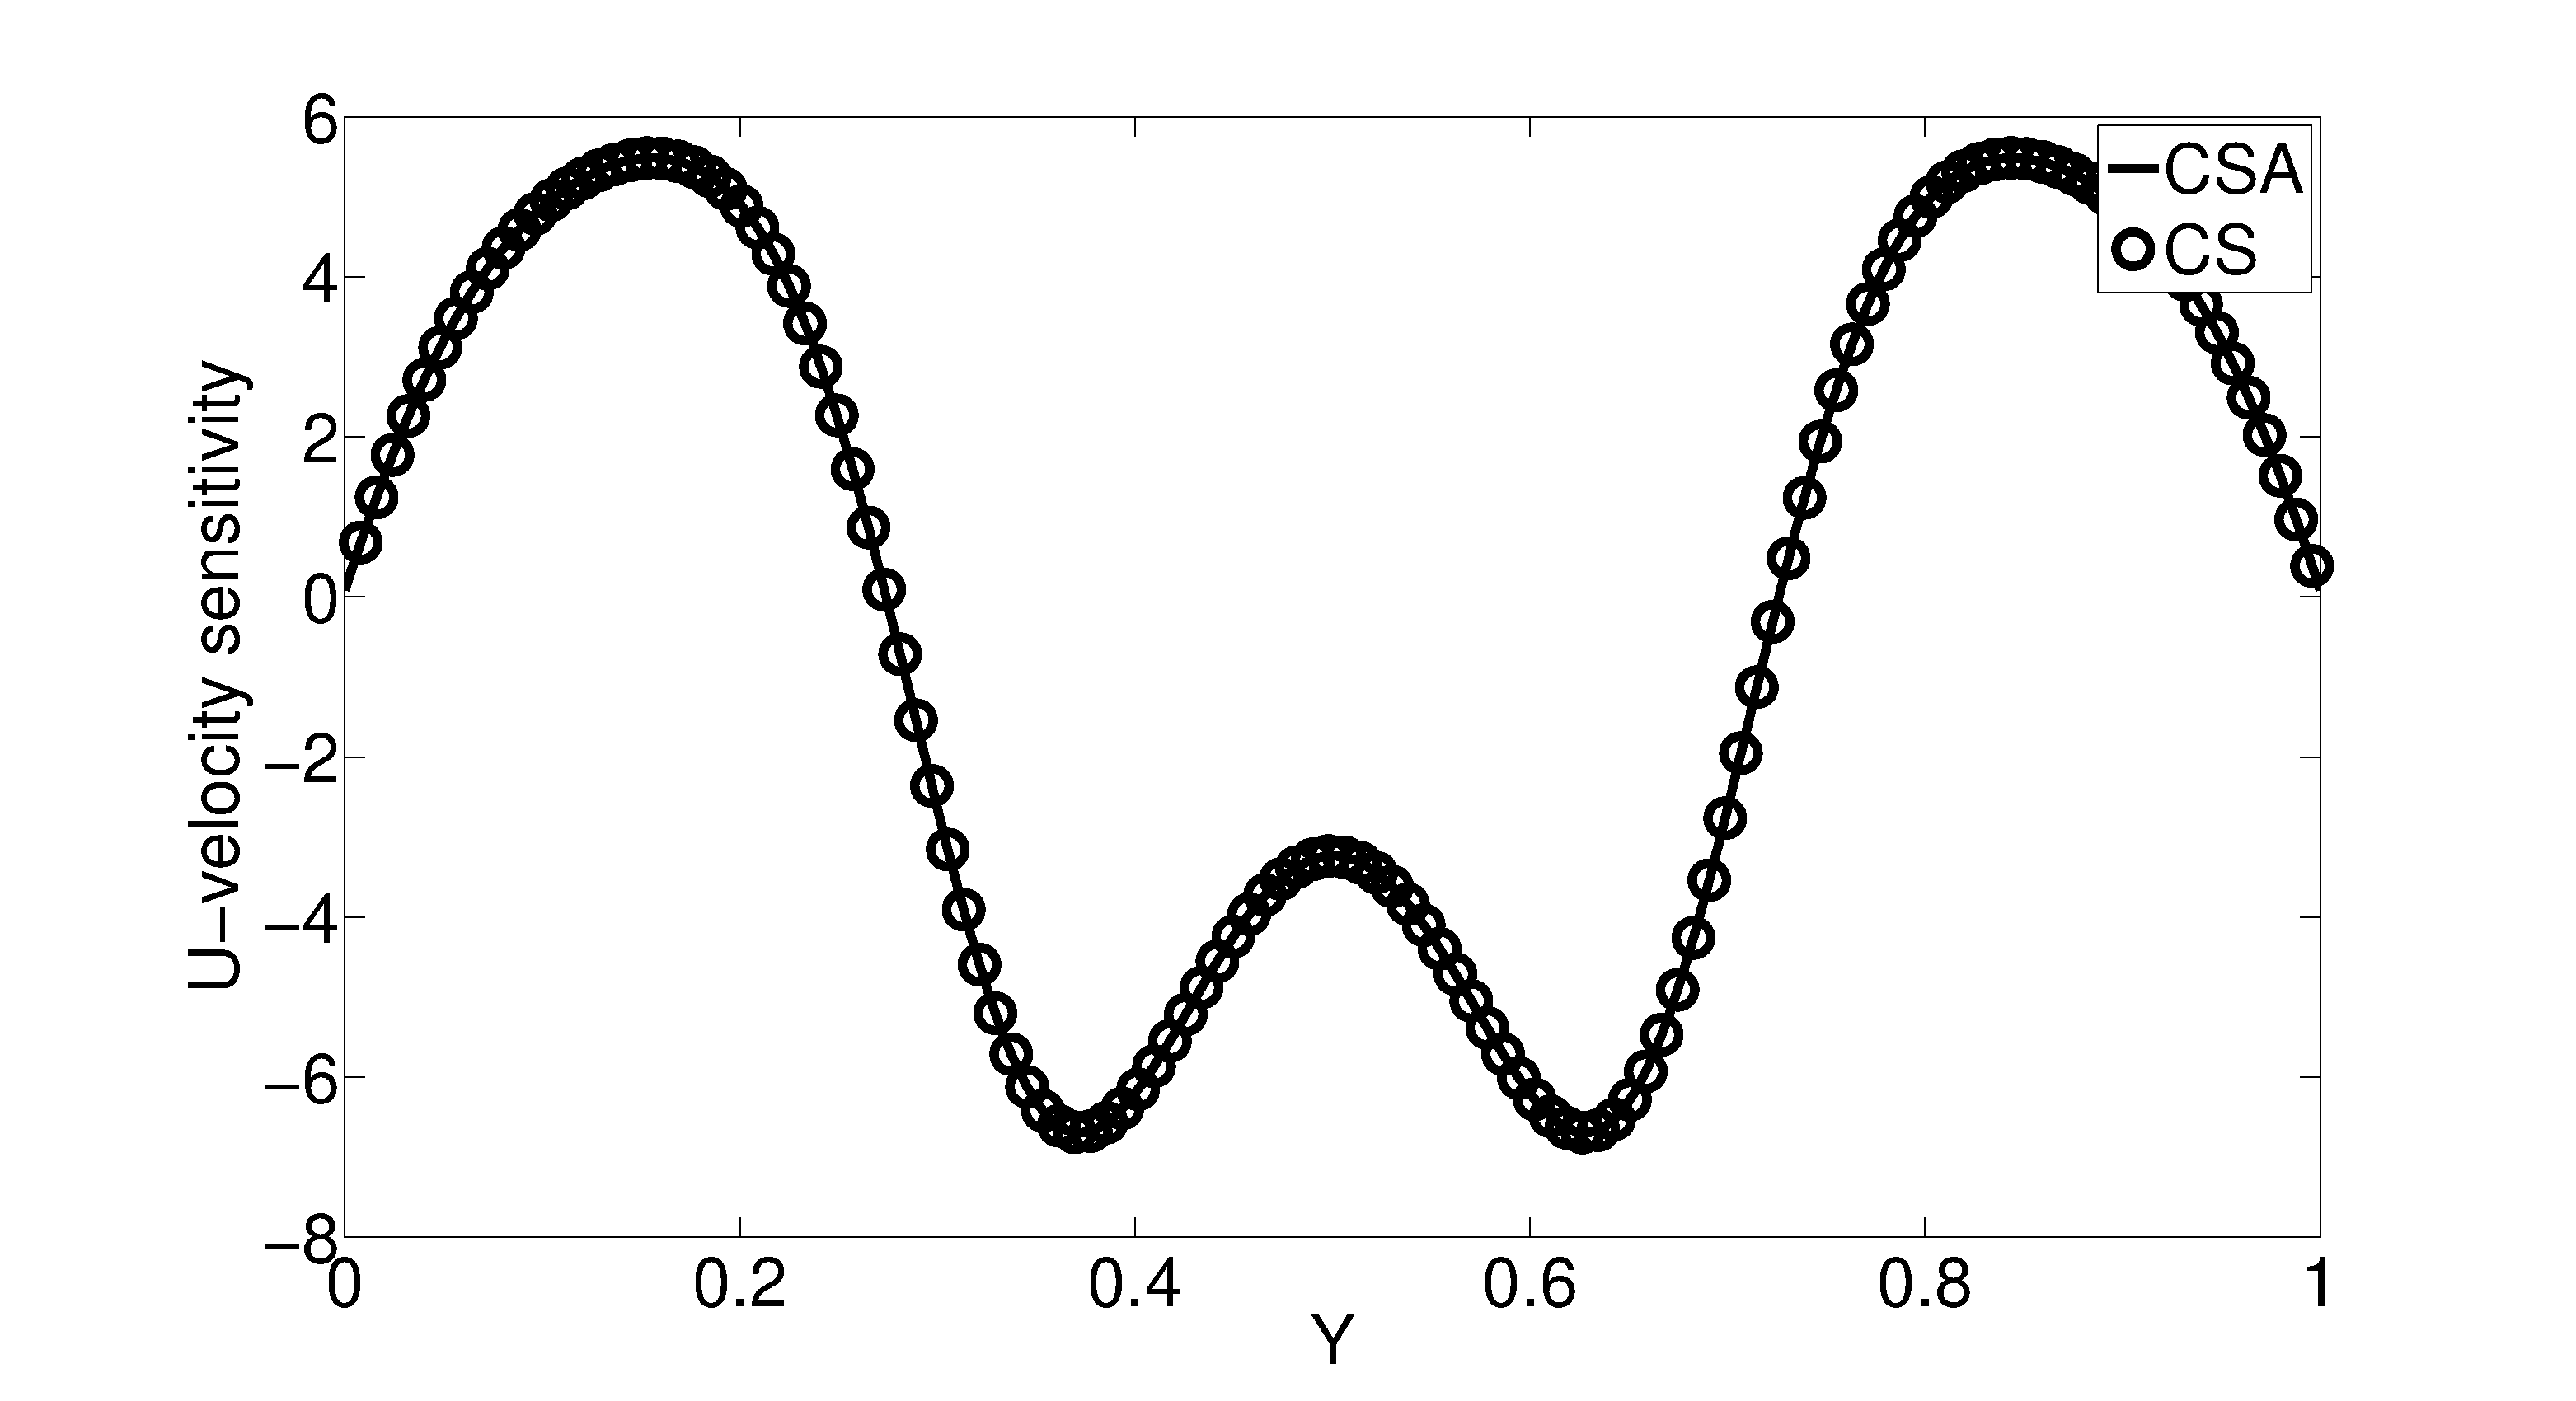
\includegraphics[height=4.0cm]{figure/cylinder/Up075_RE100.eps}
	}
	\quad
	\subfigure[x = 0.75, Re = 1000]
	{
	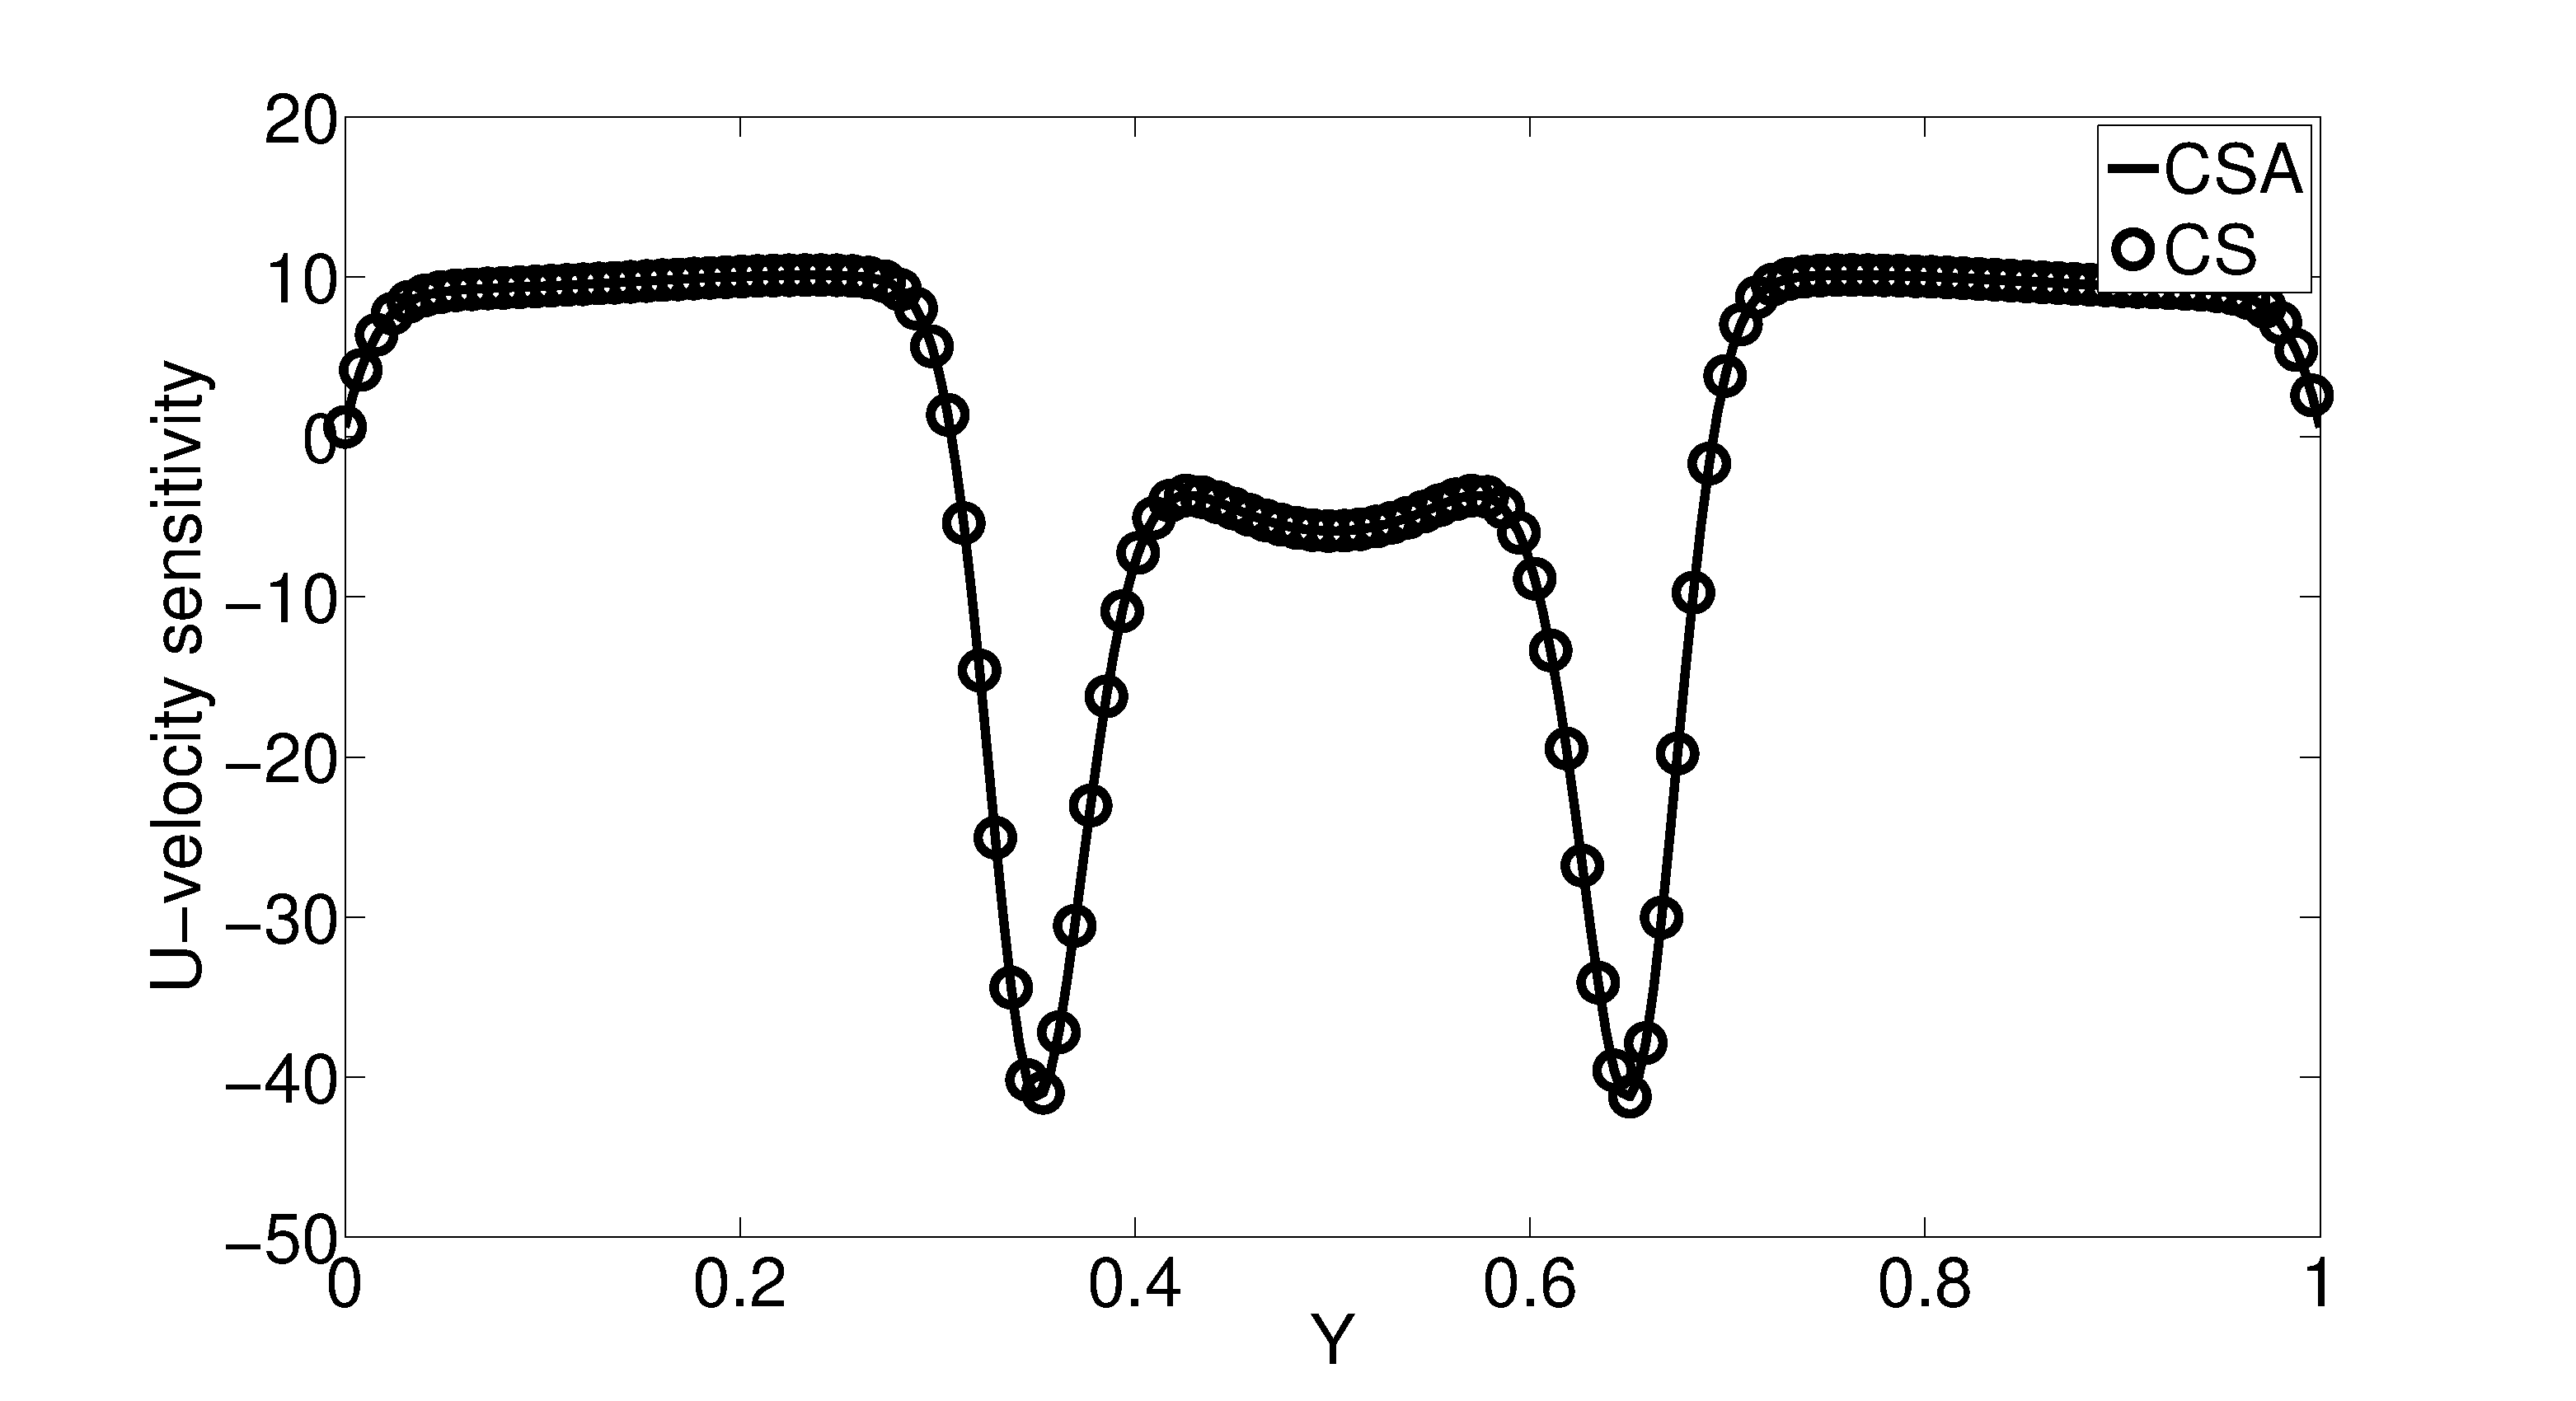
\includegraphics[height=4.0cm]{figure/cylinder/Up075_RE1000.eps}
	}
	\\
	\subfigure[x = 1.00, Re = 100]
	{
	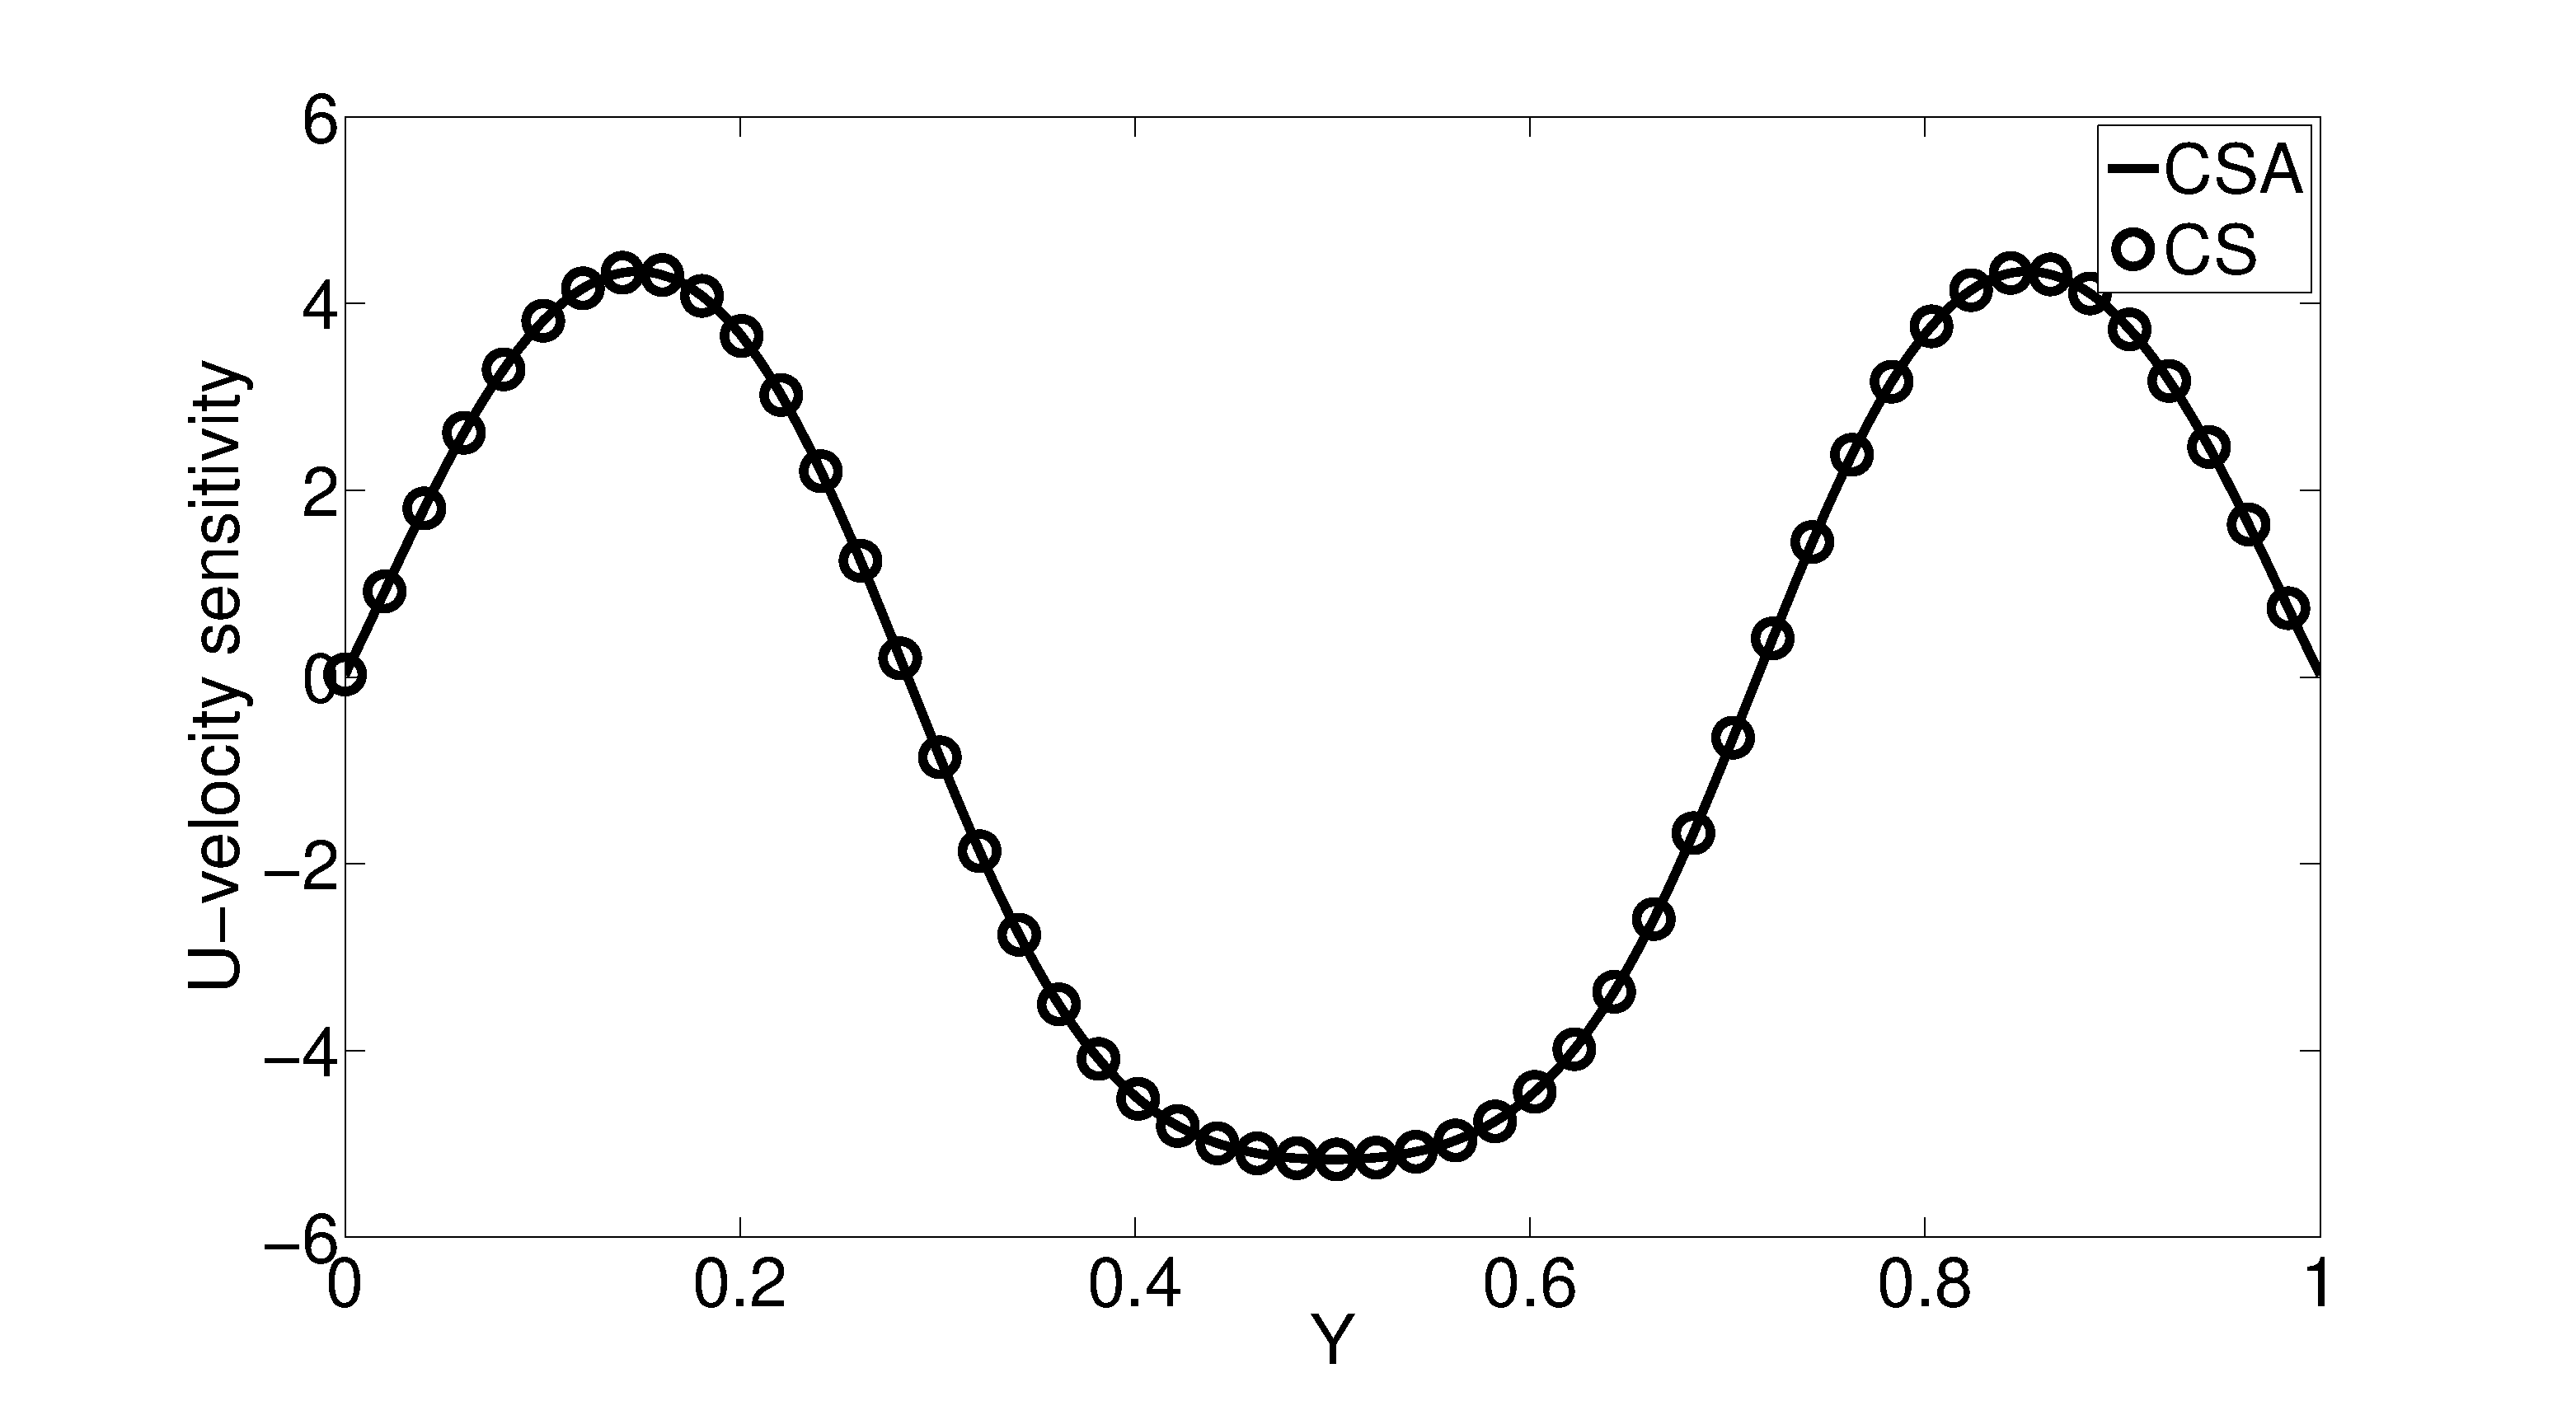
\includegraphics[height=4.0cm]{figure/cylinder/Up100_RE100.eps}
	}
	\quad
	\subfigure[x = 1.00, Re = 1000]
	{
	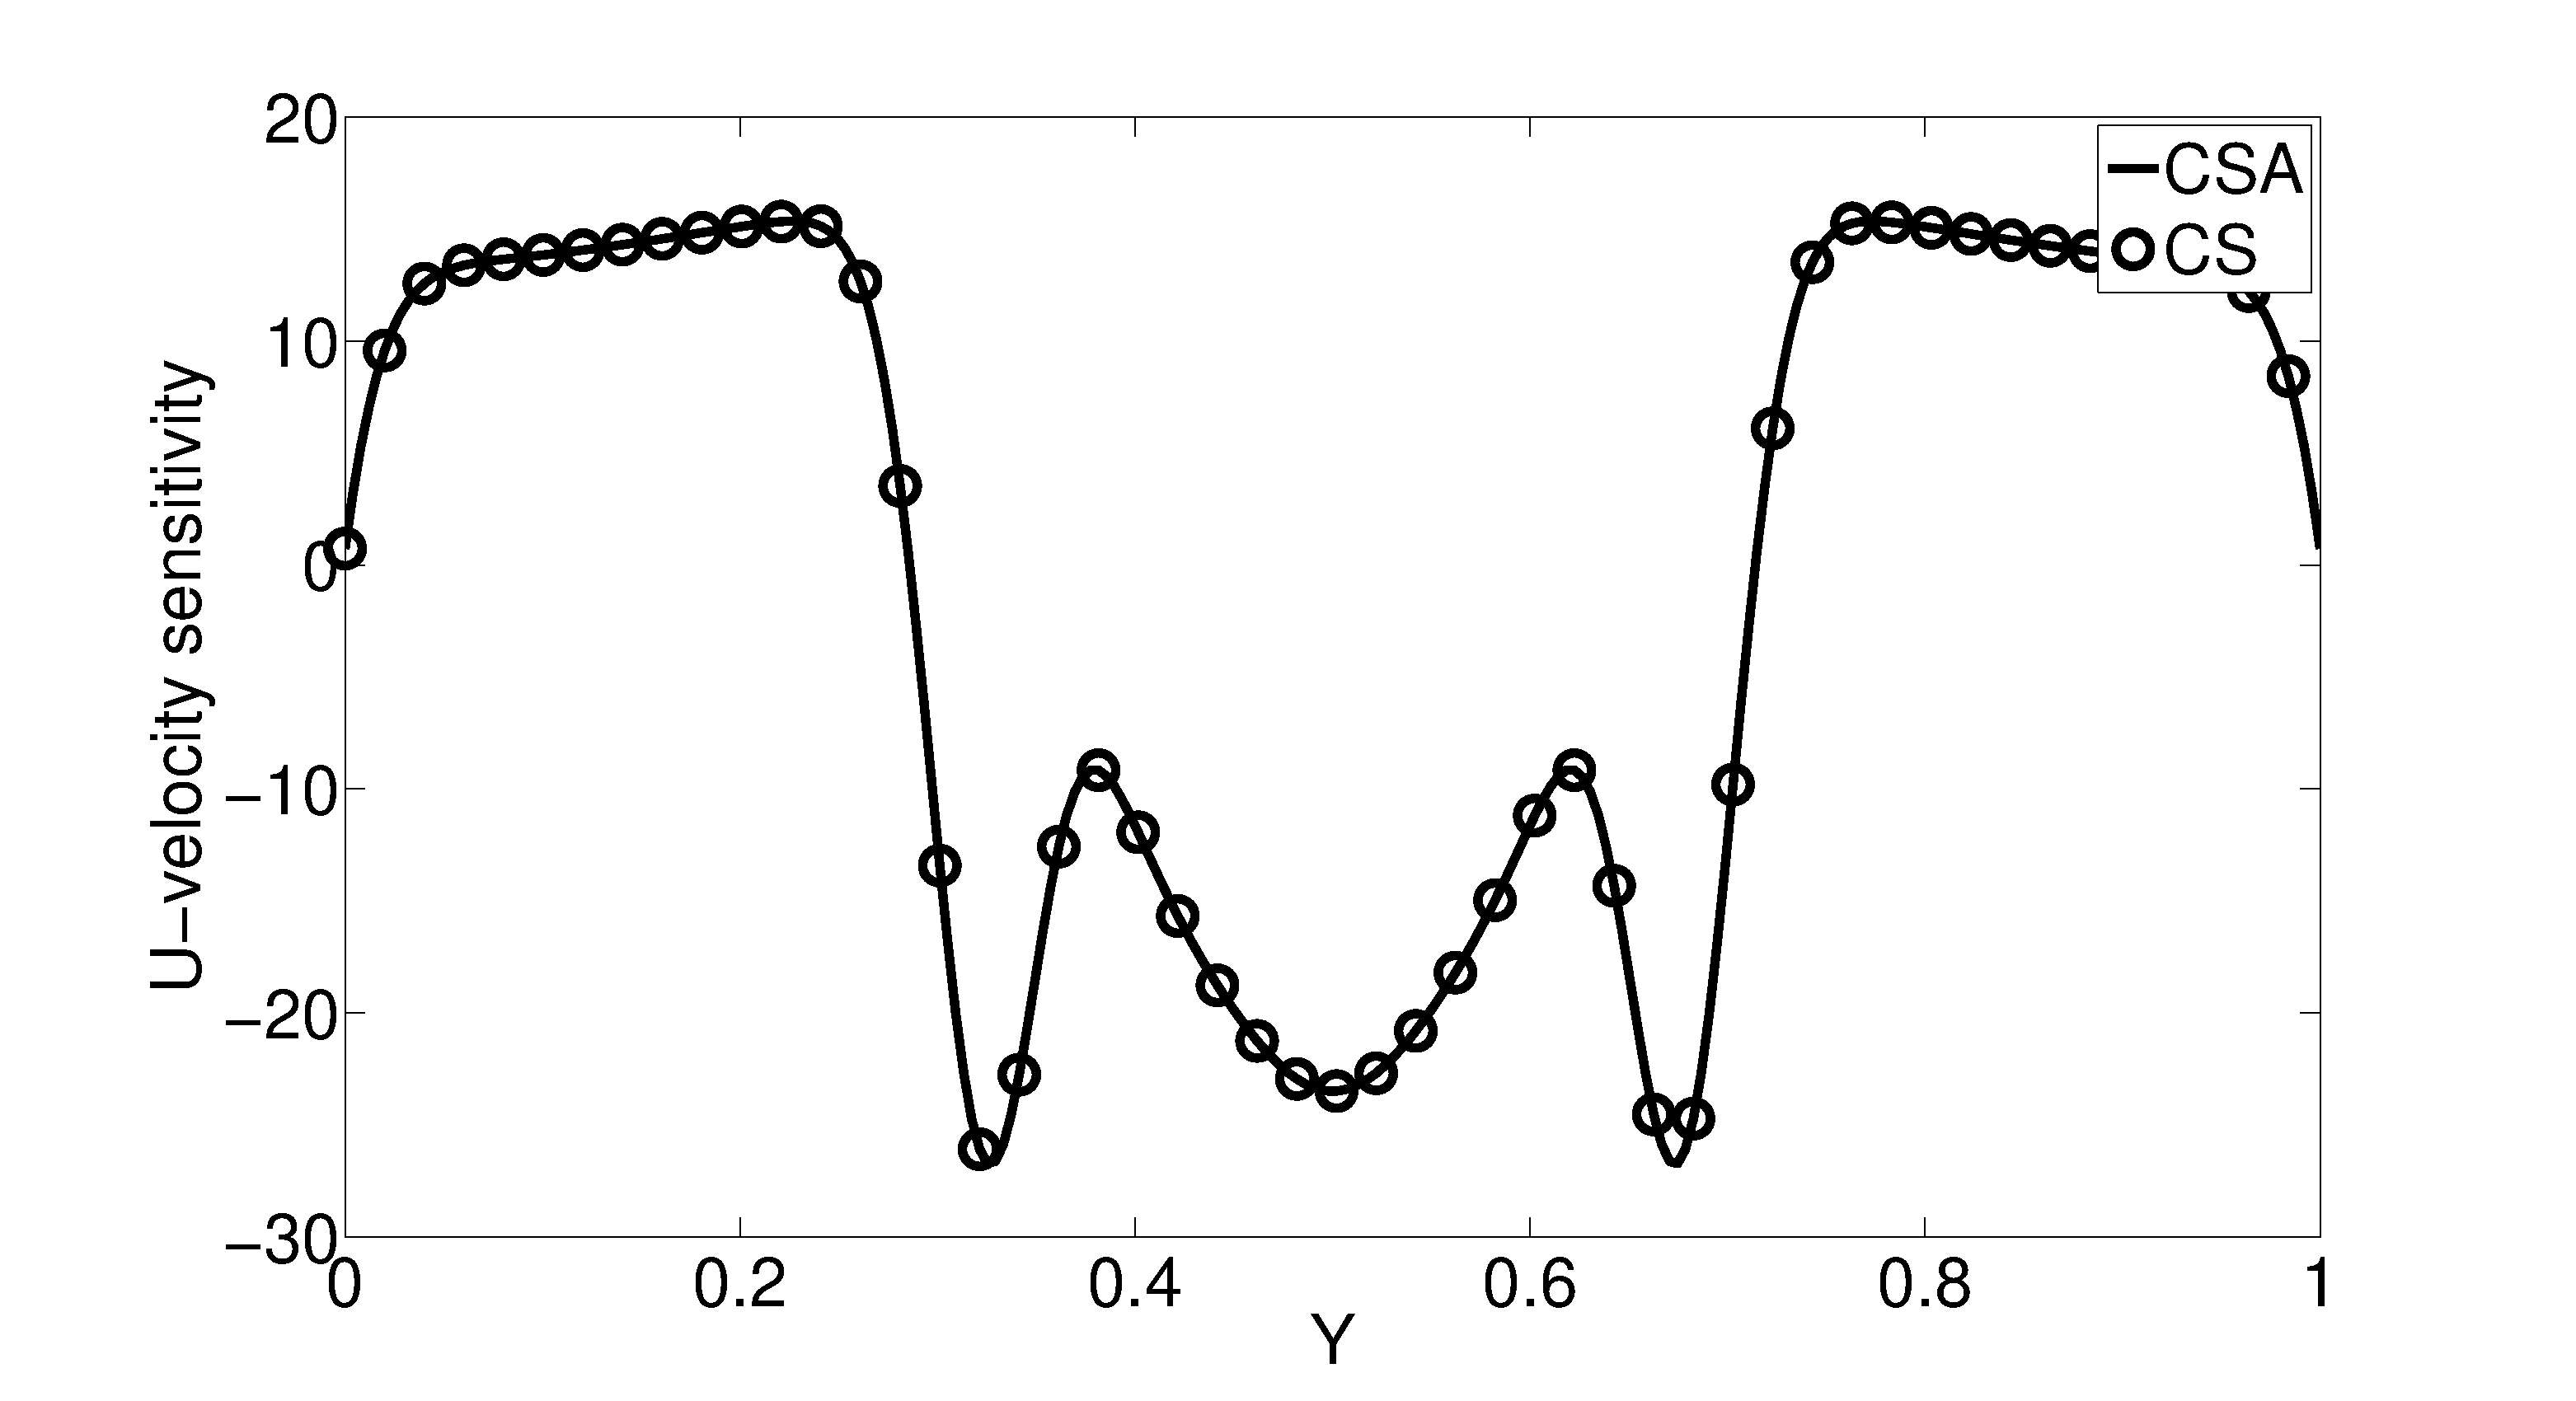
\includegraphics[height=4.0cm]{figure/cylinder/Up100_RE1000.eps}
	}
	\caption{U-velocity sensitivity to cylinder radius for different Reynolds numbers on vertical sampling line.}
	\label{fig:cylinderVelocitySensitivity}
\end{figure}
%

% -.-.-.-.-.-.-.-.-.-.-.-.-.-.-.-.-.-.-.-.-.-.-.-.-.-.-.-.-.-.-.-.-.-.-.-.-.-.-.-.-.-.-.-.-.-.-.-.-.-.-.-.-
\subsection{Linear Beam with an Airfoil}
Laminar flow over a simplified wing is selected as the second demonstration problem. The physical model for this problem is shown in Figure \ref{fig:wingModel}. The one-way fluid-solid interaction is defined by mounting the airfoil on an elastic sting. The load and moment from the aerodynamic loads are transferred to the structure through the mounting point. The beam is $4$ $m$ in length, with a cross-sectional area of $0.002$ $m^2$, and modulus of elasticity of $200$ GPa. The initial angle of attack is selected at $2$ degrees. The Reynolds number for the flow is selected as 100. The boundary conditions are defined as the inflow velocity and zero gradient of velocity at the outlet. The top and bottom walls are modelled as free-slip boundary conditions. The structure is modeled as linear Euler-Bernoulli beam. We are interested in calculating the sensitivity of the tip displacement of the structure to the shape of the airfoil.

%
\begin{figure}
	\centering
	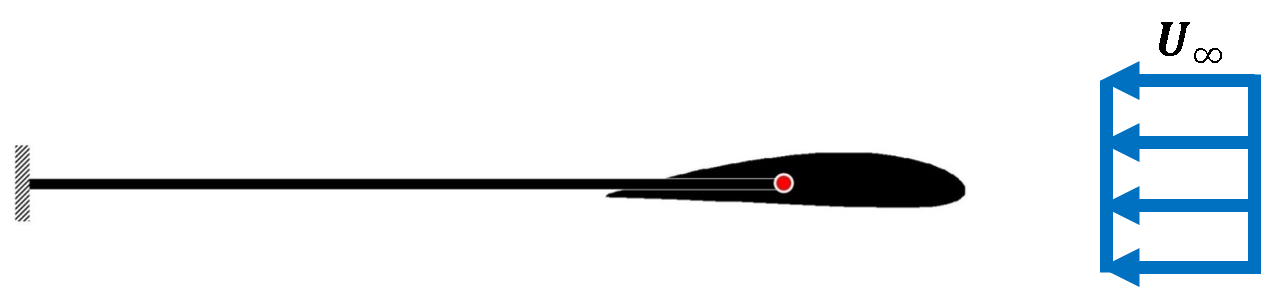
\includegraphics[height=3.75cm]{figure/airfoil/airfoil.png}
	\caption{Simplified wing model.}
	\label{fig:wingModel}
\end{figure}
%

The airfoil is defined using the Joukowsky transformation shown in Equation \eqref{eq:joukowskyTransform}, it is possible to map a circle passing through $z_1 = 1$ and containing the point $z_2 = -1$ to a curve shaped like the cross section of an airplane wing. The Joukowsky transformation is done in a complex plane.
%
\begin{equation}\label{eq:joukowskyTransform}
J(z) = z + \frac{1}{z}
\end{equation}
%
By changing the location of the original circle, it is possible to change the airfoil camber. More importantly, the airfoils have analytical definition that will be used in imposition of the force terms to the mesh cells. The effect of change in the location of original circle to the camber of the airfoil is shown in Figure \ref{fig:joukowskiChamber}. It should be noted that after generation, the airfoils are normalized such that the chord length is always equal to one.\\

%
	\begin{figure}[H]
		\centering
		\subfigure[Original circle at $(-0.1,0.1)$]
		{
		\includegraphics[height=5cm]{figure/airfoil/airfoil1.jpg}
		\label{fig:joukowskiChamber_A}
		}
		\quad
		\subfigure[Original circle at $(-0.05,0.3)$]
		{
		\includegraphics[height=5cm]{figure/airfoil/airfoil2.jpg}
		\label{fig:joukowskiChamber_B}
		}
		\caption{Airfoil definition by Joukowsky transformation (not normalized).}
		\label{fig:joukowskiChamber}
	\end{figure}
%

The pressure and u-velocity contour plots for the flow over the airfoils shown in Figure \ref{fig:joukowskiChamber} is shown in Figure \ref{fig:flowOverAirfoil}. As can be seen, the feedback forcing function is able to bring the velocity to zero on the surface of the airfoil.

%
	\begin{figure}[H]
		\centering
		\subfigure[Pressure contour]
		{
		\includegraphics[height=4cm]{figure/airfoil/airfoil1_P.png}
		\label{fig:joukowskiChamber_A}
		}
		\quad
		\subfigure[Pressure contour]
		{
		\includegraphics[height=4cm]{figure/airfoil/airfoil2_P.png}
		\label{fig:joukowskiChamber_B}
		}
		//
		\subfigure[Velocity contour]
		{
		\includegraphics[height=4cm]{figure/airfoil/airfoil1_U.png}
		\label{fig:joukowskiChamber_A}
		}
		\quad
		\subfigure[Velocity contour]
		{
		\includegraphics[height=4cm]{figure/airfoil/airfoil2_U.png}
		\label{fig:joukowskiChamber_B}
		}
		\caption{Airfoil definition by Joukowsky transformation (not normalized).}
		\label{fig:joukowskiChamber}
	\end{figure}
%

The governing equations, along with the boundary conditions, are differentiated to derive the CSEs as described in the previous section. The resulting system of equations is solved to get the sensitivity response of the system. As shown in Figure \ref{fig:joukowskiChamber}, the $y$ coordinate of the center of the original circle defines the camber. The tip displacement is proportional to the load on the structure which itself depend on the integral of the pressure over the surface of the airfoil. Therefore, to calculate the sensitivity of tip displacement it is required to calculate the sensitivity of pressure and integrate it over the boundary of the airfoil.

The sensitivity of pressure field on top and bottom surfaces of the airfoil to camber line variation is shown in Figure \ref{fig:joukowskiChamberSensitivity}. The integral of these functions are used to calculate the sensitivity of tip displacement to the change in camber of the airfoil. We used complex step method to verify the sensitivity results. As shown in Table \ref{table:sensitivity} the results of the continuum sensitivity analysis agree well with the complex step results.

%
	\begin{figure}[H]
		\centering
		\subfigure[Airfoil with original circle at $(-0.1,0.1)$]
		{
		\includegraphics[height=4.15cm]{figure/airfoil/airfoil1.eps}
		}
		\quad
		\subfigure[Airfoil with original circle at $(-0.05,0.3)$]
		{
		\includegraphics[height=4.15cm]{figure/airfoil/airfoil2.eps}
		}
		\caption{Pressure sensitivity on the surface of the airfoil.}
		\label{fig:joukowskiChamberSensitivity}
	\end{figure}
%

%
\begin{table}[H]
\centering
\begin{tabular}{c|c|c|c|c}
 & \multicolumn{1}{l|}{CSA} & \multicolumn{1}{l|}{Complex step} & \multicolumn{1}{l|}{Error} & airfoil \\ \hline
$d\delta/dy_c$ & 0.413 & 0.441 & 6.3 & (-0.1,0.1) \\ \hline
$d\delta/dy_c$ & 0.65 & 0.68 & 4.7 & (-0.05,0.3) \\
\end{tabular}
\label{table:sensitivity}
\caption{Tip displacement sensitivity to camber}
\end{table}
%
% ==========================================================================================
\section{Conclusions}
In this paper, a continuum sensitivity analysis formulation is developed for the shape sensitivity analysis for the fluid-solid interaction problems. The flow is modelled as an incompressible, laminar, and viscous fluid where the Navier-Stokes equations are used to calculate the fluid response. The solid boundaries are modelled using the continuum formulation of immersed boundary method with an addition of feedback forcing function to the Navier-Stokes equations to mimic the effect of solid boundaries. Using this approach we where able to decouple the fluid mesh from the shape of the solid boundary. This results in improving the robustness of the method since no mesh deformation is needed to handle the solid region movement. Moreover, the sensitivity analysis is simplified since the local and total sensitivities are equal for this formulation. A nonlinear mapping function is used to couple the fluid and solid domain (Eulerian and Lagrangian) grids and to map the data between these domain. As a requirement for continuum sensitivity analysis, the mapping function used need to be $\mathcal{C}^1$ continuous. This is satisfied by proposing a novel regularized delta function that has continuous derivatives. The applicability of the proposed function is showed in this paper.

This methodology is applied to two different demonstration problems. For the first problem. The sensitivity of flow to change in the radius of an immersed cylinder is calculated using the proposed method. The results show a very good comparison with the complex step results. It was shown that the method can handle flow with different Reynolds numbers. For the second demonstration problem, the one-way coupling of structural response and the fluid domain is investigated. The sensitivity of the displacement of simplified wing model to shape in the shape of the lifting surface calculated using the proposed method and compared to the complex step results. For this problem, the method was able to calculate accurate sensitivities.
% ==========================================================================================
\section*{Acknowledgements}
The authors would like to acknowledge the support provided by the Air Force Research Laboratory through contract FA8650-09-23938, the Collaborative Center for Multidisciplinary Sciences.
% References
\bibliographystyle{aiaa}
\bibliography{ref}


\end{document}